%! TeX program = lualatex
% vim: set spelllang=en:
\documentclass{manuscrit}

\institution{Université de Montréal}
\school{%
    Department of Computer Science and Operations Research\\
    \emph{Faculty of Arts and Sciences}
}
\documentkind{%
    Thesis presented for the degree\\
    of \emph{philosophiae doctor} (Ph.D.) in Computer Science
}

\title{Reconstructing the evolutionary history of genes in synteny}
\subtitle{An algebraic approach to the segmental reconciliation problem}
\author{Mattéo Delabre}

\jurypres{Sylvie Hamel}
\jurydirec{Nadia El-Mabrouk}
\jurymember{Miklós Csűrös}
\juryext{Blerina Sinaimeri}

\date{August 2026}

\begin{document}

\maketitle
\makejury
%! TeX root = ./main.tex
% vim: set spelllang=fr:
\chapter*{Abstract}

...

Keywords

\selectlanguage{french}
\tableofcontents
{\renewcommand{\addvspace}[1]{\vspace{.8ex}}\listoffigures}
\listoftables
\listofalgorithms
% \listoflistings

%! TeX root = ./main.tex
% vim: set spelllang=en:
\selectlanguage{english}
\twocolumn
\chapter*{Objects and notation}
\addcontentsline{toc}{chapter}{Objects and notation}
\markboth{\textsc{objects and notation}}{}

\paragraph{Graphs}
A graph~\(G\) is formed on a set of \emph{vertices}~\(\tnodes(G)\) connected by a set of
\emph{edges} or \emph{arcs} denoted~\(\tedges(G)\).
An edge connecting two vertices~\(a\) and~\(b\) is denoted~\(\{a, b\}\).
An arc starting at~\(a\) and ending at~\(b\) is denoted~\((a, b)\).

\paragraph{Trees}
The set of vertices of a tree~\(T\) is partitioned into the \emph{leaves} \(\tleavs(T)\) and the \emph{internal nodes} \(\tinner(T)\).
A \emph{rooted} tree has a root \(\troot(T) \in \tnodes(T)\) and is formed of arcs directed away from the root.
A tree \(T'\) \emph{displays} \(T\) if \(T\) is a minor of~\(T'\).
A \emph{forest} is a disjoint union of trees.

\paragraph{Paths}
The set of edges or arcs making up the shortest \emph{path} between two vertices \(v\) and \(w\) is denoted \(\tpath{v}{w}\).
The cardinality of this set defines the \emph{distance} between \(v\) and \(w\), denoted \(\tdist(v, w)\).

\vfill\break
\paragraph{Parenthood}
In a rooted tree \(T\), the parent of a vertex \(v\) other than \(\troot(T)\) is its unique predecessor, denoted \(\tparent(v)\).
The set of successors of an internal node \(v\), called its \emph{children}, is denoted \(\children(v)\).
These children are denoted \(v\lchild\) and \(v\rchild\) if there are two of them, or \(v\child\) if there is only one or if it is arbitrary.
The tree is \emph{binary} if the out-degree of all internal nodes is two, and \emph{partially binary} if it is one or two.

\paragraph{Descent}
If a vertex \(v\) is on the path leading from a root to a vertex \(w\), including~\(w\) itself, then \(v\) is an \emph{ancestor} of~\(w\), denoted \(v \tancs w\), and \(w\)~is a \emph{descendant} of \(v\), denoted \(w \tdesc v\).
When \(v\) and \(w\) are not comparable by \(\tdesc\), they are said to be \emph{separated}, denoted \(v \nottcomp w\).
The lowest common ancestor~(or \emph{lca}) of a set of vertices \(\{v_1, …, v_n\}\) is their ancestor furthest from the root, denoted \(\lca\{v_1, …, v_n\}\).
The subtree of \(T\) at \(v\), denoted \(\subtree{T}{v}\), is the subgraph of \(T\) formed by the descendants of \(v\).

% power set

\onecolumn

\clearpage
\thispagestyle{plain}
\vspace*{\fill}
{\raggedleft\itshape À ...\par}
\vspace*{\fill}
\clearpage

%! TeX root = ./main.tex
% vim: set spelllang=fr:
\selectlanguage{french}
\chapter*{Remerciements}

...

%! TeX root = ./main.tex
% vim: set spelllang=en:
\chapter*{Foreword}
\addcontentsline{toc}{chapter}{Foreword}
\markboth{\textsc{foreword}}{}

% Phylogénétique, introduite par l’exemple de l’évolution des gènes
% Exemples de motivations
Genes are the carriers of heredity in living organisms.
They contribute to defining their traits and can be passed on from one generation to the next.
Over time and through various events, they can evolve into different alleles and spread across multiple species.
Phylogenetics aims to trace back the evolutionary history of units such as genes, cells, or species.
These histories are valuable sources of information that can help elucidate gene functions~\parencite{Lynch2001ProbabilityPreservationNewly}, characterize the evolution of tumours~\parencite{Quinn2021SingleCellLineages} or that of pathogens~\parencite{Morel2020PhylogeneticAnalysisSars,Guindon2022EclairerOriginesCOVID19}.

% Arbres phylogénétiques et événements
A \emph{phylogenetic tree} (or \emph{phylogeny}) represents a hypothesis of evolutionary history.
Much like a family tree, a phylogenetic tree is made up of a succession of branching points and of branches along which time flows until reaching the contemporary representatives.
Each branching point of the tree corresponds to the putative divergence of an ancestor into several descendants that are free to evolve independently of one another.
The possible causes of such divergences differ according to the types of units under study; for example, genes duplicate, cells divide and species undergo speciations.

% Problème d’évolution hiérarchique
The evolution of a gene depends not only on the events directly affecting it, but also on the evolution of its host species.
Indeed, the speciation of a species causes the emergence of independent copies of its genes, one in each new species.
This relationship forms an evolutionary hierarchy between a set of \emph{evolutionary units} and their hosts.
Similar hierarchies can be found at other scales, for example between protein domains and their proteins, parasites and their hosts, or species and their habitats.
Such hierarchies also arise outside of biology, for example, between cultural elements and the populations that transmit them \parencite{Tehrani2010CophylogenyPopulationsCultures}.

% Réconciliation
To study these evolutionary hierarchies, \textcite{Goodman1979FittingGeneLineage} introduced the so-called \emph{reconciliation} method.
Relying on the topological differences and similarities between the phylogeny of a gene family and that of its host species, reconciliation makes it possible to establish which of the two each divergence relates to.
The result is a reconciled tree, a synthesis of the two trees, in which each branching point of the gene tree is annotated with the type of evolutionary event that gave rise to it.

% Problème d’évolution segmentale
When a host carries multiple families of units, their phylogenies can be reconciled individually.
This assumes, however, that the units in question have evolved independently of one another.
This assumption is invalidated in particular when the units are organized linearly within the same host, such as genes along a genome, and are affected by large-scale events.
One of the research directions of the field over the past two decades has been the integration of reconciliation methods with those allowing the study of the evolution of linear structures~\parencite{Sankoff2000DuplicationRearrangementReconciliation}.
Various extensions of the reconciliation paradigm that account for the joint evolution of several units have thus been proposed.

% Projet de recherche
The research project carried out in this thesis falls within this research direction, through the development of \emph{multiple reconciliation} methods for studying the evolution of highly conserved genome segments called \emph{syntenies}.
The contribution notably consists in identifying trade-offs between modelling power and algorithmic complexity.

\Cref{chap:reconciliation} contains a review of the relevant literature that synthesizes existing reconciliation methods.
In it, we introduce the segmental reconciliation approach that lies at the heart of the research presented thereafter.
In \cref{chap:superdtl}, we make a first contribution by allowing the inference of horizontal transfers in segmental reconciliation.
This contribution is extended to the context of unsampled species in \cref{chap:synesth}.
These extensions lead us to the need for an in-depth combinatorial study of the solution spaces associated with the problems under study.
To achieve this, we develop a unified theory of algebraic dynamic programming in \cref{chap:adp}.
This theory is put into practice on the segmental reconciliation problem in \cref{chap:adp-rec}.
Finally, the various software tools and programs developed in support of the research conducted in this thesis are presented in \cref{chap:logiciel}.

%! TeX root = ./main.tex
% vim: set spelllang=en:
\chapter{Phylogenetic reconciliation}\label{chap:reconciliation}

Two genes are said to be \emph{homologous} if they descend from a common ancestral gene.
When their divergence originates from a cospeciation with the ancestral host species, these genes are said to be \emph{orthologous}~\parencite{Fitch1970DistinguishingHomologousAnalogous}.
Conversely, the divergence can be independent of the host species: a duplication --- in which case the genes are referred to as \emph{paralogous} --- or a horizontal transfer --- they are then called \emph{xenologous}.
In particular, the identification of orthology relationships is an important step in the construction of species phylogenies, or in the study of gene function.
Indeed, orthologous genes more often share the same function than duplicated genes, which are subject to weaker selective pressure~\parencite{Lynch2001ProbabilityPreservationNewly}.

In the phylogeny of a family of homologous genes, the set of internal nodes can be partitioned according to the type of evolutionary event to which they correspond.
This partitioning makes it possible to qualify any pair of genes in the tree as orthologous, paralogous or xenologous.
The so-called \emph{reconciliation} method, introduced by \textcite{Goodman1979FittingGeneLineage}, formalized by \textcite{Page1994MapsTreesCladistic} and subsequently generalized in several ways, makes it possible to carry out such a partitioning.
It is based on the fact that genes and their host species form an evolutionary hierarchy, since the evolution of hosts affects that of the genes they contain.

In this chapter, we first introduce the reconciliation of a single family of units, which we call \emph{bilateral}, and then the various generalizations that allow \emph{multiple} reconciliations of several interdependent units.

%! TeX root = ./main.tex
% vim: set spelllang=en:
\section{Bilateral reconciliation}\label{sec:reconciliation:bilateral}

\subsection{Embedding phylogenetic trees}

An internal node~\(v\) in a phylogenetic tree~\(T\) of evolutionary units can be caused either by a codivergence with the associated host, or by a divergence independent of the host.
When~\(v\) results from a codivergence, it corresponds to an internal node in the phylogeny~\(S\) of the hosts.
Conversely, if~\(v\) is independent of the evolution of the hosts, it corresponds to a point along one of the branches of \(S\).
Finally, the leaves of \(T\) represent extant units and each correspond to a leaf of~\(S\), their host.
Such an association of \(T\) with \(S\) is called a \emph{reconciliation}.

Formally, a reconciliation is an embedding of \(T\) into \(S\), in the sense defined below.
To simplify the definition, when \(v\) corresponds to a branch of \(S\), it is associated with its endpoint.

\begin{definition}[Reconciliations]\label{definition:rec}
    Let \(T\) and \(S\) be two phylogenetic trees and \(\llmap : \tleavs(T) \onto \tleavs(S)\) a map that associates each leaf of \(T\) with its host in \(S\).
    A \emph{reconciliation} of \(T\) with~\(S\) is a map \(\rec : \tnodes(T) \onto \tnodes(S)\) that extends \(\llmap\) such that no pair of nodes \((v, w) \in \tnodes(T)^2\) is such that \(v \tancsneq w\) and \(\rec(v) \tdescneq \rec(w)\).
\end{definition}

Two examples of maps are illustrated in \cref{fig:reconciliation:strict-rec}.
The map \(\rec_1\) is an acceptable reconciliation, whereas the map \(\rec_2\) does not satisfy the condition of the definition that forbids reconciliations from \enquote{going back in time} with respect to the topology of \(S\).

\begin{figure}[htb]
    \capstart
    \centering
    %! TeX root = ../main.tex
% vim: set spelllang=fr:
\begin{tikzpicture}
    \input{fig/reconciliation/bilateral/shared-defs}

    \graph[phylogenetic tree layout, nodes={font=\small\itshape}]{
        ttree[name=ct]
    };
    \node at (0, -2.3) {\(T\)};

    \begin{scope}[shift={(3.25,0)}]
        \graph[phylogenetic tree layout, nodes={font=\small\bfseries}]{
            stree[name=ls]
        };
        \coordinate (labels) at (0, -2.3);
        \node at (labels-|ls l1s2) {\(S\)};
    \end{scope}

    \draw[separator rule] (5.15, .15) -- ++(0, -2.6);

    \begin{scope}[shift={(7.5,0)}]
        \graph[phylogenetic tree layout, nodes={font=\small\itshape}]{
            ttree[name=lt]
        };
        \node at (0, -2.3) {\(T\)};

        \begin{scope}[shift={(3.25,0)}]
            \graph[phylogenetic tree layout, nodes={font=\small\bfseries}]{
                stree[name=rs]
            };
            \coordinate (labels) at (0, -2.3);
            \node at (labels-|rs l1s2) {\(S\)};
        \end{scope}
    \end{scope}

    \path[overlaid associate=reccolor1] (ct l2s1) edge[bend left=15] (ls l2s1);
    \path[overlaid associate=reccolor1] (ct l2s2) edge[out=0, in=180] (ls l3s1);
    \path[associate=reccolor1] (ct l3s1) edge[bend left=10]
        node[above, midway] {\(\rec_1\)} (ls l3s1);

    \path[overlaid associate=reccolor2] (lt l3s1) edge[bend left=10] (rs l2s1);
    \path[overlaid associate=reccolor2] (lt l2s1) edge[bend left=15] (rs l2s1);
    \path[overlaid associate=reccolor2] (lt l2s2) edge[out=0, in=180]
        node[above, midway, reccolor2] {\(\rec_2\)} (rs l3s1);
\end{tikzpicture}

    \caption[Two examples of strict reconciliations]{
        Two associations of the phylogeny \(T\) with \(S\).
        The associations between internal nodes are represented by arrows and the associations between leaves are indicated implicitly by assigning them the same label.
    }
    \label{fig:reconciliation:strict-rec}
\end{figure}

Some units are able to migrate between two coexisting hosts.
For example, particularly in prokaryotes, horizontal transfers can cause genes to migrate between species.
In a reconciliation \(\rec\), a branch \((v, w) \in \tedges(T)\) such that \(\rec(v) \nottcomp \rec(w)\) implies that a host switch took place between two points on the path between \(\rec(v)\) and \(\rec(w)\).
Note, however, that \emph{unobservable} host switches can take place.
For example if, between \(v\) and \(w\), the unit migrated from host \(\rec(v)\) to a separated host \(\gamma\), then back again to a host descending from \(\rec(v)\) without leaving any trace among the descendants of \(\gamma\), the branch \((v, w)\) will not appear as a host-switch branch.

We call a reconciliation that does not contain any such branch \emph{strict}, since the evolution of the units then strictly follows that of their hosts.
In \cref{fig:reconciliation:strict-rec}, the reconciliation \(\rec_1\) is a strict reconciliation.
\Cref{fig:reconciliation:free-rec} gives two examples of free reconciliations.

\begin{definition}\label{definition:rec-strict}
    A reconciliation \(\rec\) of \(T\) with \(S\) is said to be \emph{strict} if all pairs of nodes
    \((v, w) \in \tnodes(T)^2\) with \(v \tancs w\) are such that \(\rec(v) \tancs \rec(w)\).
    Otherwise, \(\rec\) is said to be \emph{free}.
\end{definition}

\begin{figure}[htb]
    \capstart
    \centering
    %! TeX root = ../main.tex
% vim: set spelllang=fr:
\begin{tikzpicture}
    \input{fig/reconciliation/bilateral/shared-defs}

    \graph[phylogenetic tree layout, simple, nodes={font=\small\itshape}]{
        ttree[name=t1];
        t1 l2s2 --[transfer branch] t1 l1s4;
    };
    \node at (0, -2.3) {\(T\)};

    \begin{scope}[shift={(3.25, 0)}]
        \graph[phylogenetic tree layout, nodes={font=\small\bfseries}]{
            stree[name=s]
        };
        \coordinate (labels) at (0, -2.3);
        \node at (labels-|s l1s2) {\(S\)};
    \end{scope}

    \path[overlaid associate=reccolor3] (t1 l2s1) edge[bend left=13] (s l2s1);
    \path[associate=reccolor3] (t1 l3s1) edge[bend left=10]
        node[above, midway] {\(\rec_3\)} (s l2s1);
    \path[associate=reccolor3] (t1 l2s2) edge[bend left=10, shorten >=0pt] (s l1s1);

    \draw[separator rule] (4.8, .15) -- ++(0, -2.6);

    \begin{scope}[shift={(7.5, 0)}]
        \graph[
            phylogenetic tree layout,
            evolutionary unit length=0.44cm,
            nodes={font=\small\itshape}
        ]{
            t l4s1 / [
                coordinate,
                label={[host, reccolor4, yshift=3pt]left:α},
            ] -- {
                t l3s2 / [
                    coordinate,
                    label={[host, reccolor4, yshift=3pt]right:1},
                ] -- {
                    t l2s2 / [
                        coordinate,
                        label={[host, reccolor4]right:γ},
                        > transfer branch,
                    ] -- {
                        t l1s6 / 4 -- {},
                        t l1s5 / 3 -- {},
                    },
                    t l1s4 / 1 [> length=2],
                },
                t l3s1 / [
                    coordinate,
                    label={[host, reccolor4, yshift=3pt]left:4}
                ] -- {
                    t l1s3 / 4 [> length=2],
                    t l2s1 / [
                        coordinate,
                        label={[host, reccolor4]left:β},
                        > transfer branch,
                    ] -- {
                        t l1s2 / 2 -- {},
                        t l1s1 / 1 -- {},
                    },
                },
            },
        };
        \node[reccolor4] at (2, 0.15) {\((\rec_4)\)};
        \node at (0, -2.3) {\(T'\)};

        \begin{scope}[shift={(3.75, 0)}]
            \graph[phylogenetic tree layout, nodes={font=\small\bfseries}]{
                s l3s1 / [coordinate, label={[host]left:α}] -- {
                    s l2s2 / [coordinate, label={[host]right:γ}] -- {
                        s l1s4 / 4,
                        s l1s3 / 3,
                    },
                    s l2s1 / [coordinate, label={[host]left:β}] -- {
                        s l1s2 / 2,
                        s l1s1 / 1,
                    },
                },
            };
            \node at (0, -2.3) {\(S'\)};
        \end{scope}
    \end{scope}
\end{tikzpicture}

    \caption[Two examples of free reconciliations]{
        Two free reconciliations of the phylogenies \(T\) with \(S\) and \(T'\) with \(S'\).
        For the sake of readability, \(\rec_4\) is represented by label equalities rather than by arrows.
        The branches marked with dotted lines correspond to host switches.
    }
    \label{fig:reconciliation:free-rec}
\end{figure}

Some authors restrict \cref{definition:rec} to forbid a given internal node from having its two children associated with two separated hosts~\parencite{Nojgaard2018TimeConsistentReconciliation}.
Adding this condition guarantees that there exists a path without host switches from any internal node to a leaf.
Thus, every internal node corresponds to a divergence of which there is an extant trace.
The models we consider hereafter, however, require keeping the generality of the definition.

\subsection{Reconciled trees and reconciliation models}\label{sec:reconciliation:bilateral:model}

A reconciliation model specifies the types of events that can affect, jointly or separately, the evolution of the units and of their hosts.
An interpretation of a reconciliation under a given model is a combination of events from the model that explains its unit--host associations.
These interpretations are represented by reconciled trees labelled with the chosen events (see examples in \cref{fig:reconciliation:rec-trees}).

\begin{definition}[Reconciled trees]\label{def:reconciliation:rectree}
    Let \(T\) and \(S\) be two trees, \(\rec\) a reconciliation of \(T\) with \(S\), and \(\recmodel\) a set of event types.
    A \emph{reconciled tree} \(\rectree_{\!\recmodel}(\rec)\) (or simply \(\rectree(\rec)\) when the model used is clear from the context) is a partially binary extension of~\(T\) equipped with a map \(\exrec : \tnodes(\rectree) \onto \tnodes(S)\) that extends \(\rec\) and with a map \(\evt : \tnodes(\rectree) \onto \recmodel \cup \{\evtE\}\)
    such that \(\tleavs(T) = \{ v \in \tleavs(\rectree) \suchthat \evt(v) = \evtE \}\).
\end{definition}

Two main classes of methods exist to assess the plausibility of a reconciliation under a given model.
In \emph{parsimony} methods, the reconciliations considered most plausible are those whose interpretation invokes the fewest events of the model.
In the \emph{probabilistic} framework, it is the reconciliations whose best interpretation maximizes the likelihood that are favoured~\parencite{Doyon2011ModelsAlgorithmsPrograms}.
This thesis focuses on parsimony methods.

In parsimony, a function \(\cost : \recmodel \onto \realpos\) assigning a cost to each event type is fixed in advance.
The cost of a reconciled tree is the sum of the costs of its events.
The cost of a reconciliation is then defined as that of its most economical interpretation.
This definition gives rise to a family of combinatorial optimization problems that consist in searching for the reconciliations of minimum cost, that is, the most parsimonious ones.

\begin{problem}{\(\recmodel\)-parsimony\label{prob:reconciliation:parsimony}}
    \probinput{Phylogenies \(T\) and \(S\);
               leaf association \(\llmap : \tleavs(T) \onto \tleavs(S)\);
               costs \(\cost : \recmodel \onto \realpos\).}
    \proboutput{Minimum cost of a reconciliation of \(T\) with \(S\) under the model \(\recmodel\) and the costs \(\cost\).}
\end{problem}

Even if the phylogenies \(T\) and \(S\) under study are free of errors, the most parsimonious reconciliations do not necessarily correspond to complete or exact histories of the units concerned, since evolution rarely takes the shortest path.
On the other hand, this method has the advantage of selecting reconciliations that explain the observed data while requiring the fewest additional assumptions.

\begin{figure}[htb]
    \capstart
    \centering
    %! TeX root = ../main.tex
% vim: set spelllang=fr:
\begin{tikzpicture}
    %% Réconciliation DL
    \begin{scope}[x=.5cm, y=.8cm]
        \graph[no placement, nodes={dependent}]{
            t1l4s1 / [duplication, y=-.16] -- {
                t1l3s1 / [speciation, x=-.5, y=-1, outer sep=-.5pt] -- {
                    t1l2s1 / [speciation, x=-2.5, y=-2, outer sep=-.8pt] -- {
                        t1l1s1 / 1 [x=-4, y=-3],
                        t1l1s2 / 2 [x=-1, y=-3],
                    },
                    t1l1s3 / [loss, >loss branch, rotate=35, x=2, y=-3],
                },
                t1l3s2 / [speciation, x=.5, y=-1, outer sep=-.5pt] -- {
                    t1l2s2 / [speciation, x=-1.5, y=-2, outer sep=-.8pt] -- {
                        t1l1s4 / 1 [x=-3, y=-3],
                        t1l1s5 / [loss, >loss branch, rotate=40, x=0, y=-3],
                    },
                    t1l1s6 / 3 [x=3, y=-3, outer sep=0pt],
                },
            },
        };
        \node at (-6, -1.5) {\(\rectreeDL(\rec_1)\)};
    \end{scope}

    \draw[separator rule] (2.75, 0) -- ++(0, -2.4);

    %% Réconciliation DTL
    \begin{scope}[x=.5cm, y=.8cm, shift={(12, 0)}]
        \graph[no placement, nodes={dependent}]{
            t2l4s1 / [duplication, x=-1, y=-.75] -- {
                t2l3s1 / [speciation, x=-2.5, y=-1.5, outer sep=-.7pt] -- {
                    t2l1s1 / 1 [x=-4, y=-3],
                    t2l1s2 / 2 [x=-1, y=-3],
                },
                t2l3s2 / [speciation, x=-1.5, y=-1.5, outer sep=-.4pt] -- {
                    t2l2s1 / [transfer, x=-2.4, y=-2.4] -- {
                        t2l1s3 / 1 [x=-3, y=-3],
                        t2l1s4 anchor / [coordinate, x=1.95, y=-2.4, > transfer branch]
                            -- t2l1s4 / 3 [x=2.5, y=-3],
                    },
                    t2l1s5 / [loss, >loss branch, rotate=32, x=0, y=-3],
                },
            },
        };
        \coordinate (t2lroot) at (0, -.16);
        \node at (6, -1.5) {\(\rectreeDTL(\rec_3)\)};
    \end{scope}

    \begin{pgfonlayer}{hostnodes}
        \node[host leaf node, fit=(t1l1s1)(t1l1s4)] (s1l1s1) {};
        \node[host leaf node, fit=(t1l1s2)(t1l1s5)] (s1l1s2) {};
        \node[host leaf node, fit=(t1l1s3)(t1l1s6)] (s1l1s3) {};
        \node[host node, fit=(t1l2s1)(t1l2s2)] (s1l2s1) {};
        \node[host node, fit=(t1l3s1)(t1l3s2)] (s1l3s1) {};

        \node[host leaf node, fit=(t2l1s1)(t2l1s3)] (s2l1s1) {};
        \node[host leaf node, fit=(t2l1s2)(t2l1s5)] (s2l1s2) {};
        \node[host leaf node, fit=(t2l1s4), inner xsep=.2cm] (s2l1s3) {};
        \node[host node, fit=(t2l3s1)(t2l3s2)] (s2l2s1) {};
        \node[host node, fit=(t2lroot), inner xsep=.5cm, inner ysep=.25cm] (s2l3s1) {};
    \end{pgfonlayer}

    \foreach \i in {1,2} {
        \begin{pgfonlayer}{hostedges}
            \path[host edge] (s\i l2s1.east) -- (s\i l3s1.east) -- (s\i l3s1.west) -- (s\i l2s1.160);
            \path[host edge] (s\i l1s1.-10) -- (s\i l2s1.east) -- (s\i l2s1.160) -- (s\i l1s1.165);
            \path[host edge] (s\i l1s2.15) -- (s\i l2s1.east) -- (s\i l2s1.west) -- (s\i l1s2.190);
            \path[host edge] (s\i l1s3.15) -- (s\i l3s1.east) -- (s\i l3s1.west) -- (s\i l1s3.190);
        \end{pgfonlayer}
    };

    \begin{pgfonlayer}{hostedges}
        \path[host edge terminal] (s1l3s1.east) -- ($(s1l3s1.east)+(0, 1)$)
            -- ($(s1l3s1.west)+(0, 1)$) -- (s1l3s1.west);
    \end{pgfonlayer}
\end{tikzpicture}

    \caption[Two examples of reconciled trees]{
        Reconciled trees for the reconciliations \(\rec_1\) and \(\rec_3\) (from \cref{fig:reconciliation:strict-rec,fig:reconciliation:free-rec}) under the duplication-loss~(\(\recmodelDL\)) and duplication-transfer-loss~(\(\recmodelDTL\)) models respectively.
        Each tree is overlaid on the outline of the host phylogeny so as to reflect the association of nodes given by the reconciliation.
        Each circle~{\showspeciation} represents a codivergence event~(\(\evtS\)),
        each square~{\showduplication} a duplication~(\(\evtD\)),
        each diamond~{\showtransfer} a transfer~(\(\evtT\)),
        and each upward-opening half-circle~{\showloss} a loss~(\(\evtL\)).
    }
    \label{fig:reconciliation:rec-trees}
\end{figure}

\paragraph{Duplication and loss~\textup{\parencite{Goodman1979FittingGeneLineage,Page1994MapsTreesCladistic}}}
This model comprises three event types, \(\recmodelDL = \{\evtD, \evtL, \evtS\}\).
The divergence of a unit is explained by its duplication~(\(\evtD\)) or its cospeciation with its host~(\(\evtS\)), and the absence of a unit in a descendant host is explained by a loss~(\(\evtL\)).
Each node \(v \in \tnodes(\rectree)\) of a reconciled tree under this model is such that:
\begin{compactitemize}
\item if \(\evt(v) = \evtD\), then \(v\) is an internal node and \(\exrec(v) = \exrec(v\lchild) = \exrec(v\rchild)\);
    \item if \(\evt(v) = \evtL\), then \(v\) is a leaf;
    \item if \(\evt(v) = \evtS\), then \(v\) and \(\exrec(v)\) are internal nodes and \(\{\exrec(v\lchild), \exrec(v\rchild)\} = \{\exrec(v)\lchild, \exrec(v)\rchild\}\).
\end{compactitemize}
Loss events introduce additional leaves into the reconciled tree compared to the tree of units.
They make it possible to interpret situations where the two endpoints of a branch are associated with two non-adjacent hosts, by inserting a sequence of speciations and losses into this branch.
\Cref{fig:reconciliation:rec-trees} presents an example of an interpretation of a reconciliation under the \(\recmodelDL\) model in which such a sequence of losses is used.

The cost functions considered for this model usually set \(\cost(\evtS) = 0\).
Consequently, searching for minimum-cost reconciliations amounts to maximizing the number of codivergences between \(T\) and \(S\).
This choice is motivated by the fact that each \(\evtS\)~event relies on the speciation of a host, an event already postulated by the tree \(S\) given as input.

\paragraph{Host switch~\textup{\parencite{Tofigh2011SimultaneousIdentificationDuplications,Ranwez2016InferringGeneDuplications}}}
The model \(\recmodelDTL = \{\evtD, \evtT, \evtL, \evtS\}\) extends the \(\recmodelDL\) model to integrate the possibility of host switches and thus allow free reconciliations to be interpreted.
In addition to the three event types defined previously, for an internal node \(v \in \tinner(\rectree)\) under this model, if \(\evt(v) = \evtT\), then \(\exrec(v) = \exrec(v\lchild)\) and \(\exrec(v) \nottcomp \exrec(v\rchild)\), or else \(\exrec(v) = \exrec(v\rchild)\) and \(\exrec(v) \nottcomp \exrec(v\lchild)\).
An example of an interpretation of a reconciliation under the \(\recmodelDTL\) model is given in \cref{fig:reconciliation:rec-trees}.

In this model, a host switch can be immediately followed by a loss, thus leaving no trace in the original host.
This observation, initially ignored in the work of \textcite{Tofigh2011SimultaneousIdentificationDuplications}, can lead to the construction of significantly different interpretations \parencite{Ranwez2016InferringGeneDuplications}.
It also makes it possible to interpret reconciliations containing nodes whose two children are associated with hosts separated from that of their parent.
However, taking it into account leads to an increase in the number of co-optimal solutions in the associated optimization problem~\parencite{Weiner2021ImprovedDuplicationTransfer}.

\paragraph{Unsampled hosts~\textup{\parencite{Szoelloesi2013LateralGeneTransfer,Weiner2021ImprovedDuplicationTransfer}}}
The phylogeny \(S\) is necessarily incomplete since it only gives information about the hosts of the units of~\(T\).
The internal nodes leading only to hosts absent from this sample are therefore missing.
In the context of free reconciliations, it is possible for a unit to evolve in a part of the phylogeny located outside the sample before later being transferred to a sampled host.
To represent this possibility, the \(\recmodelDTLx\) model adds an additional event, denoted \(\evtTX\), to the \(\recmodelDTL\) model.
For an internal node \(v \in \tinner(\rectree)\) under this model, if \(\evt(v) = \evtTX\), then \(\exrec(v) = \exrec(v\lchild)\) and \(\exrec(v) \tancs \exrec(v\rchild)\), or else \(\exrec(v) = \exrec(v\rchild)\) and \(\exrec(v) \tancs \exrec(v\lchild)\).
This event offers an alternative to inserting sequences of losses to interpret a reconciliation branch whose two endpoints are associated with non-adjacent hosts.
This can provide a more parsimonious interpretation for some reconciliations, as illustrated in~\cref{fig:reconciliation:rec-dtlx}.

\begin{figure}[htb]
    \capstart
    \centering
    %! TeX root = ../main.tex
% vim: set spelllang=fr:
\begin{tikzpicture}
    %% Réconciliation DL
    \begin{scope}[x=.5cm, y=.8cm]
        \graph[no placement, nodes={dependent}]{
            t1l4s1 / [duplication, y=-.16] -- {
                t1l3s1 / [speciation, x=-.5, y=-1, outer sep=-.45pt] -- {
                    t1l2s1 / [speciation, x=-2.5, y=-2, outer sep=-.8pt] -- {
                        t1l1s1 / 1 [x=-4, y=-3, >shorten >=-3pt],
                        t1l1s2 / 2 [x=-1, y=-3, >shorten >=-4pt],
                    },
                    t1l1s3 / 3 [x=2, y=-3, >shorten >=-3pt],
                },
                t1l3s2 / [speciation, x=.5, y=-1, outer sep=-.45pt] -- {
                    t1l2s2 / [speciation, x=-1.5, y=-2, outer sep=-.8pt] -- {
                        t1l1s4 / 1 [x=-3, y=-3, >shorten >=-3pt],
                        t1l1s5 / [loss, >loss branch, rotate=40, x=0, y=-3],
                    },
                    t1l1s6 / [loss, >loss branch, rotate=40, x=3, y=-3],
                },
            },
        };
    \end{scope}

    \draw[separator rule] (2.75, 0) -- ++(0, -2.4);

    %% Réconciliation DTL
    \begin{scope}[x=.5cm, y=.8cm, shift={(12, 0)}]
        \graph[no placement, nodes={dependent}]{
            t2l4s1 / [speciation, x=0.5, y=-.16, outer sep=-.7pt] -- {
                t2l3s1 / [speciation, x=-.8, y=-.9, outer sep=-.7pt] -- {
                    t2l2s1 / [speciation, x=-2.25, y=-1.75, outer sep=-.7pt] -- {
                        t2l1s1 / 1 [x=-4, y=-3, >shorten >=-3pt],
                        t2l1s2 / 2 [x=-.5, y=-3, >shorten >=-4pt],
                    },
                    t2l1s3 / 3 [x=2, y=-3, >shorten >=-3pt],
                },
                t2l3s2 / [transfer, x=3.75, y=-2.4] -- {
                    t2l2s2 / [coordinate, x=-2.4, y=-2.4, > transfer branch] --
                        t2l1s4 / 1 [x=-3, y=-3, >shorten >=-3pt],
                    t2l1sx / [coordinate, x=5, y=-3.3, > dotted],
                },
            },
        };
    \end{scope}

    \begin{pgfonlayer}{hostnodes}
        \node[host leaf node, fit=(t1l1s1)(t1l1s4)] (s1l1s1) {};
        \node[host leaf node, fit=(t1l1s2)(t1l1s5)] (s1l1s2) {};
        \node[host leaf node, fit=(t1l1s3)(t1l1s6)] (s1l1s3) {};
        \node[host node, fit=(t1l2s1)(t1l2s2)] (s1l2s1) {};
        \node[host node, fit=(t1l3s1)(t1l3s2)] (s1l3s1) {};

        \node[host leaf node, fit=(t2l1s1)(t2l1s4)] (s2l1s1) {};
        \node[host leaf node, fit=(t2l1s2), inner xsep=.075cm] (s2l1s2) {};
        \node[host leaf node, fit=(t2l1s3), inner xsep=.075cm] (s2l1s3) {};
        \node[host node, fit=(t2l2s1), inner xsep=.15cm] (s2l2s1) {};
        \node[host node, fit=(t2l3s1), inner xsep=.15cm] (s2l3s1) {};
        \node[host node, fit=(t2l4s1), inner xsep=.15cm] (s2l4s1) {};
        \node[ellipse, fit=(t2l1sx), inner sep=.3cm] (s2l1sx) {};
    \end{pgfonlayer}

    \begin{pgfonlayer}{hostedges}
        \path[host edge] (s1l2s1.east) -- (s1l3s1.east) -- (s1l3s1.west) -- (s1l2s1.160);
        \path[host edge] (s1l1s1.-10) -- (s1l2s1.east) -- (s1l2s1.160) -- (s1l1s1.165);
        \path[host edge] (s1l1s2.15) -- (s1l2s1.east) -- (s1l2s1.west) -- (s1l1s2.190);
        \path[host edge] (s1l1s3.15) -- (s1l3s1.east) -- (s1l3s1.west) -- (s1l1s3.190);
        \path[host edge terminal] (s1l3s1.east) -- ($(s1l3s1.east)+(0, 1)$)
            -- ($(s1l3s1.west)+(0, 1)$) -- (s1l3s1.west);

        \path[host edge unsampled] (s2l4s1.15) -- (s2l1sx.east) -- (s2l1sx.west) -- (s2l4s1.west);
        \path[host edge] (s2l3s1.-10) -- (s2l4s1.-10) -- (s2l4s1.160) -- (s2l3s1.160);
        \path[host edge] (s2l2s1.-10) -- (s2l3s1.-10) -- (s2l3s1.160) -- (s2l2s1.160);
        \path[host edge] (s2l1s1.-10) -- (s2l2s1.east) -- (s2l2s1.160) -- (s2l1s1.165);
        \path[host edge] (s2l1s2.15) -- (s2l2s1.east) -- (s2l2s1.west) -- (s2l1s2.190);
        \path[host edge] (s2l1s3.15) -- (s2l3s1.east) -- (s2l3s1.west) -- (s2l1s3.190);
    \end{pgfonlayer}
\end{tikzpicture}

    \caption[Alternative interpretations of the same reconciliation under two models]{
        Two alternative interpretations of the same reconciliation under the \(\recmodelDL\) and \(\recmodelDTLx\) models.
        In the reconciled tree on the right, the event at the root is a \(\evtTX\) event, which is represented as a speciation followed by a transfer inside a hypothetical unsampled (hatched) branch of the host phylogeny.
    }
    \label{fig:reconciliation:rec-dtlx}
\end{figure}

\paragraph{Other models}
Extensions of reconciliation to take \emph{incomplete lineage sorting}~(ILS) into account have been proposed by \textcite{Rasmussen2012UnifiedModelingGene,Wu2013MostParsimoniousReconciliation,Chan2017InferringIncompleteLineage}.
This phenomenon occurs when speciations that are close in time cause the emerging species to inherit distinct subsets of units.
As an alternative to \(\recmodelDL\)-type models, \textcite{Goodman1979FittingGeneLineage} proposed a model integrating the possibility for a gene to be activated or deactivated by a regulatory mechanism, which makes it possible to limit the inference of superfluous losses.
Finally, the dating of the host phylogeny, which imposes an additional constraint on host switches, can be integrated into the models allowing this type of event~\parencite{Tofigh2011SimultaneousIdentificationDuplications}.

\subsection{Time consistency}

Host switches imply temporal constraints, since the donor host and the recipient host of each switch must have been able to coexist for the event to occur.
Thus, for a reconciled tree to represent a realistic evolutionary scenario, it must satisfy the following constraints, imposed by the topology of the host tree and by the events of the reconciliation model
\parencite{Stolzer2012InferringDuplicationsLosses,Ma2017DTLReconciliationRepair}.

\begin{definition}[Time consistency of a reconciled tree]\label{def:reconciliation:time-cons}
    A reconciled tree \(\rectree(\rec)\) is said to be \emph{time-consistent} if there exists a preorder \(\succeq_\tau\) on \(\tnodes(\rectree) \cup \tnodes(S)\) such that:
    \begin{condition}
        \item \(s \succ_\tau s\child\) for each branch \((s, s\child) \in \tedges(S)\); \label{def:reconciliation:time-cons:hosts}
        \item \(v \succeq_\tau v\child\) for each branch \((v, v\child) \in \tedges(\rectree)\); \label{def:reconciliation:time-cons:events}
        \item \(\tparent(\exrec(v)) \succ_\tau v \succeq_\tau \exrec(v)\) for each node \(v \in \tnodes(\rectree)\) such that \(\exrec(v) \neq \troot(S)\), otherwise \(v \succeq_\tau \exrec(v)\); \label{def:reconciliation:time-cons:events-hosts}
        \item \(v \succeq_\tau v\child\) and \(v\child \succeq_\tau v\) for each branch \((v, v\child) \in \tedges(\rectree)\) such that \(\exrec(v) \nottcomp \exrec(v\child)\). \label{def:reconciliation:time-cons:host-switch} \qedhere
    \end{condition}
\end{definition}

Intuitively, a reconciled tree is time-consistent if it is possible to draw a diagram of it similar to those of \cref{fig:reconciliation:rec-trees,fig:reconciliation:rec-dtlx}.
In such a representation, all branches are oriented along the same time axis (\cref{def:reconciliation:time-cons:hosts,def:reconciliation:time-cons:events}).
Each codivergence is overlaid on the node of the corresponding host tree and each divergence is placed along the corresponding branch (\cref{def:reconciliation:time-cons:events-hosts}).
Finally, host-switch branches are drawn orthogonally to the time axis (\cref{def:reconciliation:time-cons:host-switch}).

\begin{figure}[htb]
    \capstart
    \centering
    \begin{tikzpicture}[scale=1.25]
    \begin{scope}
        \input{fig/reconciliation/bilateral/time-seq-error}
    \end{scope}
    \draw[separator rule] (3.5, -.2) -- ++(0, 2.45);
    \begin{scope}[shift={(5, 0)}]
        \input{fig/reconciliation/bilateral/time-seq-valid}
    \end{scope}
\end{tikzpicture}

    \caption[Examples of time inconsistencies]{
        Examples of time inconsistencies.
        \emph{(Left.)}
        Two alternative interpretations of the same reconciliation under the~\(\recmodelDTL\) model.
        The interpretation on the left is time-inconsistent whereas the one on the right is consistent.
        These diagrams are generated by the \emph{superrec2} software, presented in \cref{sec:logiciel:superrec2}, which automatically detects whether a reconciled tree is time-consistent.
        \emph{(Right.)}
        A reconciliation for which there exists no time-consistent interpretation.
    }
    \label{fig:reconciliation:time-cons}
\end{figure}

The \textsc{Bellman--Ford} algorithm makes it possible to check whether a given reconciled tree satisfies the conditions of \cref{def:reconciliation:time-cons} in \(\bigo((|\tnodes(\rectree)| + |\tnodes(S)|)^2)\) time~\parencite[section~22.4]{Cormen2022IntroductionAlgorithms}.
When the conditions are satisfied, this algorithm furthermore makes it possible to obtain a minimal total order satisfying the constraints and thus to help draw a diagram of the tree.

A reconciliation \(\rec\) is said to be \emph{acyclic} in a model \(\recmodel\) if there exists a time-consistent reconciled tree \(\rectree_{\!\recmodel}(\rec)\).
For example, the reconciliation \(\rec_3\) of \cref{fig:reconciliation:free-rec} is acyclic because of the interpretation given in \cref{fig:reconciliation:rec-trees}.
Some acyclic reconciliations, such as the one on the left of \cref{fig:reconciliation:time-cons}, have both consistent and inconsistent interpretations.

The following lemma, adapted from \textcite[theorem 1]{Tofigh2009InferringDuplicationsLateral}, makes it possible to check whether a reconciliation is acyclic in the \(\recmodelDTL\) model without enumerating all of its interpretations.

\begin{lemma}[Acyclicity of a reconciliation]\label{lem:reconciliation:rec-cons}
    A reconciliation \(\rec\) is acyclic in the \(\recmodelDTL\) model if and only if there exists a preorder \(\succeq_\sigma\) on \(\tnodes(S)\) such that:
    \begin{condition}
        \item \(s \succ_\sigma s\child\) for each branch \((s, s\child) \in \tedges(S)\); \label{lem:reconciliation:rec-cons:hosts}
        \item \(\tparent(\rec(v)) \succ_\sigma \rec(v'\child)\) for all branches \((v, v\child), (v', v'\child) \in \tedges(T)\) with \(v_c \tancs v_c'\) and \(\rec(v) \neq \troot(S)\).
            \label{lem:reconciliation:rec-cons:host-switch}
    \end{condition}
\end{lemma}
\begin{proof}
    Suppose that there exists an interpretation of \(\rec\) with a preorder \(\succeq_\tau\) satisfying the conditions of \cref{def:reconciliation:time-cons}.
    Observe that \cref{def:reconciliation:time-cons:hosts} of the definition is identical to \cref{lem:reconciliation:rec-cons:hosts} of the lemma, which is thus trivially satisfied.
    Moreover, let \((v, v\child), (v', v'\child) \in \tedges(T)\) be two branches such that \(v\child \tancs v'\child\) and \(\rec(v) \neq \troot(S)\).
    By \cref{def:reconciliation:time-cons:events,def:reconciliation:time-cons:events-hosts} of the definition, \(\tparent(\rec(v)) = \tparent(\exrec(v)) \succ_\tau v \succeq_\tau v\child\) and \(v'\child \succeq_\tau \exrec(v'\child) = \rec(v'\child)\) and therefore \(\tparent(\rec(v)) \succ_\tau \rec(v'\child)\).
    Thus, the restriction of~\(\succeq_\tau\) to the nodes of \(S\) gives a preorder satisfying the conditions of the lemma.

    Conversely, suppose that there exists a preorder \(\succeq_\sigma\) satisfying the conditions of the lemma and take a linear extension \(\succeq_\sigma'\) of it.
    We construct an interpretation \(\exrec\) of \(\rec\), not necessarily parsimonious, associated with a total order \(\succeq_\tau\) that completes \(\succeq_\sigma'\) and satisfies \cref{def:reconciliation:time-cons}.

    Following a prefix order on \(T\), for each host-switch branch \((v, v\child) \in \tedges(T)\) such that \(\rec(v) \nottcomp \rec(v\child)\), let us consider the time interval in which this switch can occur.
    This interval is bounded by \(b(v\child)\) and \(a(v\child)\), defined as
    \begin{align*}
        b(v\child) &= \min_{\succeq_\tau}\left(\{v' \mid v'\child \tancsneq v\child \text{ and } \exrec(v') \nottcomp \exrec(v'\child)\} \cup \{\tparent(\exrec(v))\}\right) \\
        a(v\child) &= \max_{\succeq_\tau}\left(\{\exrec(v'\child) \mid v\child \tancs v'\child \text{ and } \exrec(v') \nottcomp \exrec(v'\child)\} \cup \{\exrec(v)\}\right).
    \end{align*}
    Now note that \(b(v\child) \succ_\tau a(v\child)\).
    Let \((v^b, v^b\child) \in \tedges(T)\) and \((v^a, v^a\child) \in \tedges(T)\) be two branches such that \(v^b\child \tancsneq v\child\), \(v\child \tancs v^a\child\), \(\exrec(v^b) \nottcomp \exrec(v^b\child)\), and \(\exrec(v^a) \nottcomp \exrec(v^a\child)\).
    Observe that \(a(v^b\child) \succeq_\tau a(v\child)\), on the one hand because \(v^b\child \tancsneq v\child \tancs v'\child\), and on the other hand because \(\exrec(v''\child) \succeq_\tau \exrec(v)\), where \((v'', v''\child)\) is the most recent host-switch branch before \((v, v\child)\).
    Now, inductively, we can assume that \(v^b\) has~been placed such that \(v^b \succ_\tau a(v^b\child) \succeq_\tau a(v\child)\).
    By \cref{lem:reconciliation:rec-cons:host-switch} of the lemma, \(\tparent(\exrec(v)) \succ_\tau \exrec(v^a\child)\).
    Finally, \(\tparent(\exrec(v)) \succ_\tau \exrec(v)\) by \cref{lem:reconciliation:rec-cons:hosts} of the lemma.

    To interpret the host-switch branch \((v, v\child)\),
    it is subdivided by inserting two consecutive intermediate nodes \(v_0\) and \(v_1\).
    The node \(v_0\) is marked as a transfer event associated with the host \(\exrec(v_0) = \rec(v)\), leading on the one hand to a loss and on the other hand to the node~\(v_1\) resulting from the transfer.
    The non-empty interval between \(b(v\child)\) and \(a(v\child)\) makes it possible to date these nodes such that \(b(v\child) \succ_\tau v_0 =_\tau v_1 \succ_\tau a(v\child)\).
    This choice inductively satisfies \cref{def:reconciliation:time-cons:events} since \(v^b \succeq_\tau b(v\child) \succ_\tau v_0 =_\tau v_1\).
    \Cref{def:reconciliation:time-cons:events-hosts} of the definition is satisfied for~\(v_0\) since \(\tparent(\exrec(v)) \succeq_\tau b(v\child) \succ_\tau v_0 \succ_\tau a(v\child) \succeq_\tau \exrec(v)\).
    Finally, \(\lca\{\exrec(v), \exrec(v\child)\} \succeq_\tau \tparent(\exrec(v)) \succeq_\tau b(v\child)\), so there exists a host \(t\) such that \(\lca\{\exrec(v), \exrec(v\child)\} \tancsneq t \tancs \exrec(v\child)\) and \(\tparent(t) \succ_\tau v_1 \succeq_\tau t\).
    The node \(v_1\) is then associated with such a host \(t\), which satisfies \cref{def:reconciliation:time-cons:events-hosts} of the definition for~\(v_1\).

    Finally, the other nodes \(v \in \tinner(T)\) are marked as duplications and the branches \((v, v\child)\) such that \(\exrec(v) \tancsneq \exrec(v\child)\) are subdivided by inserting enough speciations and losses and by choosing suitable dates.
\end{proof}

For example, in the reconciliation \(\rec_5\) of \cref{fig:reconciliation:time-cons}, a first transfer branch from host~2 to host~3 is followed by another transfer from host~3 to host~\(\beta\).
These two transfers, in order to satisfy \cref{lem:reconciliation:rec-cons:host-switch} of the previous lemma, require that \(\beta >_\sigma \beta\), so there exists no interpretation of \(\rec_5\) that is time-consistent.

A reconciliation can, however, be cyclic without containing two transfers following one another.
For example, for the reconciliation \(\rec_4\) of \cref{fig:reconciliation:free-rec}, the transfer branch from host~4 to host~\(\beta\) requires that \(\gamma \succ_\sigma \beta\) whereas the one from host~1 to host~\(\gamma\) requires that \(\beta \succ_\sigma \gamma\).
Thus, the reconciliation \(\rec_4\) is also cyclic by the previous lemma.

A weaker version of \cref{lem:reconciliation:rec-cons:host-switch}, which did not consider pairs of transfers following one another, was initially stated by \textcite{Charleston1998JunglesNewSolution}.
As shown by \textcite{Tofigh2009InferringDuplicationsLateral}, this condition is incomplete, in particular because it does not identify reconciliation \(\rec_5\) as cyclic.

\subsection{Complexity of \(\recmodel\)-parsimony problems}

As suggested by the following two statements, the space of strict reconciliations is more easily explorable and more restricted than the general space of reconciliations.

\begin{remark}
    All strict reconciliations are acyclic.
\end{remark}

\begin{lemma}\label{lemma:strict-rec-space}
    If \(\rec\) is a strict reconciliation of \(T\) with \(S\) then, for every internal node \(v \in \tnodes(T)\),
    \(\rec(v) \tancs \lca\left\{ \llmap(l) \suchthat l \in \tleavs(\subtree{T}{v}) \right\}\).
\end{lemma}
\vspace{-1em}
\begin{proof}
    Let \(\rec\) be a reconciliation of \(T\) with \(S\) and suppose that an internal node \(v \in \tnodes(T)\) is such that
    \(\rec(v) \nottancs \lca\left\{ \llmap(l) \suchthat l \in \tleavs(\subtree{T}{v}) \right\}\).
    There therefore exists \(w \in \tleavs(\subtree{T}{v})\) such that \(\rec(v) \nottancs \llmap(w)\)
    and therefore such that \(\rec(v) \not\tancs \rec(w)\).
    Hence \(\rec\) is not strict.
\end{proof}

\vspace{-.5em}
The strict reconciliation that associates each internal node of \(T\) with the most recent possible host in~\(S\) is denoted \(\reclca\) and defined by \(
    \reclca(v) = \lca\left\{ \llmap(l) \suchthat l \in \tleavs(\subtree{T}{v}) \right\}
\).

Since the \(\recmodelDL\) model excludes any possibility of host switch, the optimal reconciliations lie within the space of strict reconciliations (see lemma~\labelcref{lemma:strict-rec-space}).
The reconciliation~\(\reclca\) is always a solution under this model.
Moreover, provided that \(\cost(\evtL) > 0\), it is the unique solution~\parencite{Chauve2009NewPerspectivesGene}.
Computing~\(\reclca\) only requires linear time and space in the size of \(T\)~\parencite{Zhang1997MirkinMuchnikSmith}.
The \(\recmodelDL\)-parsimony problem is therefore polynomial.

Unlike the \(\recmodelDL\) model, there may exist several optimal reconciliations under the \(\recmodelDTL\) model and the reconciliation \(\reclca\) is not necessarily one of them.
Moreover, a natural constraint for this problem is to only take acyclic reconciliations into consideration.
However, this constraint makes the associated decision problem NP-complete, as shown by \textcite{Tofigh2011SimultaneousIdentificationDuplications} through a reduction from the maximum acyclic subgraph problem.

To circumvent this difficulty, in what follows, we will allow cyclic reconciliations.
We will also evaluate the cost of a reconciliation as that of its least costly interpretation, even if the latter is inconsistent.
Thus, the reconciliation \(\rec_4\) of \cref{fig:reconciliation:free-rec} becomes acceptable and the reconciliation of \cref{fig:reconciliation:time-cons} costs only two transfer events, even though a loss is necessary to make it a time-consistent interpretation.

These modifications give the problem an optimal substructure: a solution for the subtree \(\subtree{T}{v}\) is always an assembly of two solutions for \(\subtree{T}{v\lchild}\) and \(\subtree{T}{v\rchild}\).
\Cref{alg:reconciliation:dtl-parcimonie} exploits this property to solve the problem efficiently.

\newcommand{\fndtl}{\mathrm{cost}}
\newcommand{\varspe}{\mathrm{Spe_{LR}}}
\newcommand{\varsperl}{\mathrm{Spe_{RL}}}
\newcommand{\vardup}{\mathrm{Dup}}
\newcommand{\varhgt}{\mathrm{Tra_L}}
\newcommand{\varhgtr}{\mathrm{Tra_R}}
\newcommand{\varhgtlr}{\mathrm{Tra_{LR}}}

\begin{algorithm}
    \capstart
    \begin{algorithmic}[1]\setstretch{1.25}
        \Require{%
            \(T\) and \(S\), two phylogenies;\\
            \(\llmap : \tleavs(T) \onto \tleavs(S)\), an association between their leaves;\\
            \(\cost : \recmodelDTL \onto \realpos\), a cost for the \(\recmodelDTL\) events.
        }
        \Ensure{Minimum cost of a reconciliation of \(T\) with \(S\) under the \(\recmodelDTL\) model, including cyclic reconciliations.}
        \Function{cost}{\(v\), \(\sigma\)}
            \If{\(v \in \tleavs(T)\)}
                \Return \(0\) {\algorithmicif} \(\sigma = \llmap(v)\)\textbf{,} {\algorithmicelse} \(\infty\) \;
            \EndIf
            \State \(\displaystyle\varspe \gets \min_{\sigma' \tdesc \sigma\lchild} \{
                \fndtl(v\lchild, \sigma') + \cost(\evtL) \cdot \tdist(\sigma\lchild, \sigma')
            \} + \min_{\sigma'' \tdesc \sigma\rchild} \{
                \fndtl(v\rchild\kern1pt, \sigma'') + \cost(\evtL) \cdot \tdist(\sigma\rchild\kern1pt, \sigma'')
            \}\)
            \State \(\displaystyle\varsperl \gets \min_{\sigma' \tdesc \sigma\rchild} \{
                \fndtl(v\lchild, \sigma') + \cost(\evtL) \cdot \tdist(\sigma\rchild\kern1pt, \sigma')
            \} + \min_{\sigma'' \tdesc \sigma\lchild} \{
                \fndtl(v\rchild\kern1pt, \sigma'') + \cost(\evtL) \cdot \tdist(\sigma\lchild, \sigma'')
            \}\)
            \State \(\displaystyle\vardup \gets \cost(\evtD) + \min_{\sigma' \tdesc \sigma} \{
                \fndtl(v\lchild, \sigma') + \cost(\evtL) \cdot \tdist(\sigma, \sigma')
            \} + \min_{\sigma'' \tdesc \sigma} \{
                \fndtl(v\rchild\kern1pt, \sigma'') + \cost(\evtL) \cdot \tdist(\sigma, \sigma'')
            \}\)
            \State \(\displaystyle\varhgt \gets \cost(\evtT) + \min_{\sigma' \nottcomp \sigma} \{
                \fndtl(v\lchild, \sigma')
            \} + \min_{\sigma'' \tdesc \sigma} \{
                \fndtl(v\rchild\kern1pt, \sigma'') + \cost(\evtL) \cdot \tdist(\sigma, \sigma'')
            \}\)
            \State \(\displaystyle\varhgtr \gets \cost(\evtT) + \min_{\sigma' \tdesc \sigma} \{
                \fndtl(v\lchild, \sigma') + \cost(\evtL) \cdot \tdist(\sigma, \sigma')
            \} + \min_{\sigma'' \nottcomp \sigma} \{
                \fndtl(v\rchild\kern1pt, \sigma'')
            \}\)
            \State \Return \(\min\{\varspe, \varsperl, \vardup, \varhgt, \varhgtr\}\)
        \EndFunction
        \State \Return \(\min_{\sigma \in \tnodes(S)}\Call{cost}{\troot(T), \sigma}\)
    \end{algorithmic}
    \caption{
        Recursive algorithm for the \(\recmodelDTL\)-parsimony problem.
        \label{alg:reconciliation:dtl-parcimonie}
    }
\end{algorithm}

The function \(\Call{cost}{v, \sigma}\) computes the minimum cost of a reconciliation of \(\subtree{T}{v}\) with \(S\) such that \(v\) is associated with the given host \(\sigma\).
To do so, recursive calls are used to obtain the minimum cost of reconciliations of \(\subtree{T}{v\lchild}\) and \(\subtree{T}{v\rchild}\) with \(S\) when \(v\lchild\) and \(v\rchild\) are associated with different hosts \(\sigma'\) and \(\sigma''\) of \(S\).
The assembly of sub-reconciliations in the algorithm is based on the following observations:
\begin{compactitemize}
    \item \(\evt(v) = \evtS\) only if \(\sigma\) is an internal node and \(\sigma'\) and \(\sigma''\) are each in one of the two subtrees \(\subtree{S}{\sigma\lchild}\) and \(\subtree{S}{\sigma\rchild}\) (variables \(\varspe\) and \(\varsperl\));
    \item \(\evt(v) = \evtD\) only if \(\sigma'\) and \(\sigma''\) descend from \(\sigma\) (variable \(\vardup\));
    \item \(\evt(v) = \evtT\) only if \(\sigma'\) or \(\sigma''\) are separated from \(\sigma\) (variables \(\varhgt\) and \(\varhgtr\));
    \item except for transfer branches, loss events must be inserted for each host traversed between \(\sigma\), \(\sigma'\) and \(\sigma''\) in order to comply with the model (terms in \(\cost(\evtL) \cdot \hdots\)).
\end{compactitemize}

\Cref{alg:reconciliation:dtl-parcimonie} can be transformed to use a dynamic programming table that stores the values of \(\fndtl(v, \sigma)\), thereby avoiding repeating the same computation several times.
Letting \(n = \lvert\tnodes(T)\rvert\) and \(m = \lvert\tnodes(S)\rvert\), the algorithm thus transformed has a time complexity of \(\bigo(nm^2)\) and a space complexity of \(\bigo(nm)\)~\parencite{Tofigh2011SimultaneousIdentificationDuplications}.
The time complexity can be reduced to \(\bigo(nm)\) without modifying the space complexity~\parencite{Bansal2012EfficientAlgorithmsReconciliation}.
The \(\recmodelDTL\)-parsimony problem is therefore polynomial.

\Cref{alg:reconciliation:dtl-parcimonie} can be extended to the \(\recmodelDTLx\) model without changing its complexity.
To do so, it suffices to add, for each of lines~3 to~7, a case in which the terms in \(\cost(\evtL) \cdot \hdots\) are replaced by the invocation of a \(\evtTX\) event.

\subsection{Applications of reconciliation methods}

Bilateral reconciliation allows the study of the joint evolution of evolutionary units and their hosts.
The algorithms described in the previous section make it possible to obtain information about these evolutionary relationships from the respective phylogenies of the units and of the hosts.
Under some evolutionary models, such as the~\(\recmodelDTL\) model, several distinct solutions may, however, be optimal in the sense of the parsimony criterion.
Moreover, the execution of these algorithms depends on the costs set for each event type, and varying these costs modifies the optimal solutions.
It is therefore not sufficient to analyse a single solution returned by a single parameterization of an algorithm.
For a meaningful analysis, the solution space must be explored to quantify the extent to which these solutions agree on the different parts of the inferred scenario~\parencite[see][]{Doyon2009SpaceGeneSpeciesTrees,Weiner2021ImprovedDuplicationTransfer}.
We will address these questions from the angle of algebraic dynamic programming in \cref{chap:adp,chap:adp-rec}.

The phylogenies expected as input to the algorithms are sometimes known with limited precision, or are even unknown.
Reconciliation can provide a criterion for improving these phylogenies.
For example, reconciliation can be used to infer an unknown species tree from a set of trees of several gene families~\parencite[see][p.~72--73]{Guigo1996ReconstructionAncientMolecular,Page1994MapsTreesCladistic}.
The underlying problem being NP-complete~\parencite{Ma2000GeneTreesSpecies}, this application of reconciliation relies on heuristics.
In some cases, particularly when there are uncertainties in its construction, the phylogeny of the units may contain polytomies, that is, internal nodes having more than two descendants.
Reconciliation can then be used as a criterion to \emph{resolve} these polytomies by searching for the binary tree that yields a lower reconciliation score~\parencite{Lafond2016EfficientNonBinary}.

%! TeX root = ./main.tex
% vim: set spelllang=en:
\section{Multiple reconciliation}

Some hosts carry several families of units.
To reconstruct the respective histories of these families, bilateral reconciliation methods could be applied to them individually.
This approach would, however, assume that the units under study evolve independently of one another, which is in particular not the case for some genes.
Genes are indeed organized linearly along the genome of their species and affected by genome-scale events.
These events modify the organization and the composition of the genome, acting simultaneously on several of its genes.

The evolution of linear structures, shaped by rearrangements and duplications, is mainly studied in the context of comparative genomics.
The \emph{genome phylogeny} problem consists in reconstructing the most plausible phylogenetic tree for a set of genomes, by associating each internal node with an ancestral genome.
This problem comes in a \emph{\enquote{large}} version, where the topology of the tree and the ancestral genomes are inferred simultaneously, and a \emph{\enquote{small}} version, in which the topology is fixed and only the ancestral genomes remain to be determined~\parencite[for a review of these problems, see][]{ElMabrouk2012AnalysisGeneOrder}.

To address these problems, \textcite{Sankoff2000DuplicationRearrangementReconciliation} proposed combining the methods developed to analyse evolution at the scale of gene families with those for the scale of genomes.
The information recovered by reconciliation, in particular orthology relationships, could indeed guide the study of the evolution of genomes containing several copies of the same gene family.
Conversely, integrating the genomic scale into reconciliation would make it possible to take into account the interdependence of the evolution of genes.
The research objective is thus the development of methods capable of reconstructing the joint history of several gene families~\parencite[see also][]{Chauve2013DuplicationRearrangementReconciliation}.

To do so, an intermediate level can be integrated into the bilateral reconciliation model, placed between the scale of genes and that of species, in order to model evolution at the genomic scale.
In what follows, we compare two existing approaches based on this idea according to their modelling capacity and their algorithmic complexity.

\subsection{Adjacency reconciliation}

The linear organization of a set of units can be represented by a set of adjacencies between pairs of units.
For example, the genome \(\{(a, b, c), (d, e)\}\) made up of two chromosomes and five genes corresponds to the three adjacencies \(\{\{a, b\}, \{b, c\}, \{d, e\}\}\).
This representation notably makes it easier to model rearrangement events, since it suffices to act on the adjacencies at the border of the segment moved by the event.
The DeCo approach (for \enquote{Detection of Coevolution}), introduced by \textcite{Berard2012EvolutionGeneNeighborhoods}, extends reconciliation to integrate the evolution of adjacencies between pairs of dependent units.

Suppose that a forest \(\gtrees\) of phylogenies of dependent units and the phylogeny \(S\) of their hosts are known.
An adjacency \(\{a, b\}\) between two internal nodes of \(\gtrees\) is an assertion stating that the two divergences occurred simultaneously in the same host and that the copy of \(a\) is an immediate neighbour of \(b\) in the structure of this host.

\begin{definition}[Adjacencies]\label{definition:adj}
    An \emph{adjacency} on a set \(L\) is a pair \(\{a, b\} \subseteq L\) such that \(a \neq b\).
    A map \(f : L \onto M\) \emph{respects} such an adjacency if \(f(a) = f(b)\).
    The set of all possible adjacencies respected by~\(f\) is denoted~\(\alladjs(f)\).
\end{definition}

Suppose that the set of adjacencies between the leaves of \(\gtrees\) is also known.
An adjacency reconciliation of \(\gtrees\) with \(S\) (see \cref{fig:reconciliation:adj-rec}) is a reconciliation of each tree of \(\gtrees\) with \(S\) together with a set of ancestral adjacencies leading to the adjacencies between the leaves.

\begin{definition}[Adjacency reconciliations]\label{definition:adjrec}
    Let \(\gtrees\) be a phylogenetic forest and \(S\) a phylogenetic tree.
    Let \(\llmap : \tleavs(\gtrees) \onto \tleavs(S)\) be a map and \(\lladjset \subseteq \alladjs(\llmap)\) a set of adjacencies.
    An \emph{adjacency reconciliation} of \(\gtrees\) with \(S\) is a pair \(\tup{\rec, \adjset}\),
    where \(\rec\) is a map extending~\(\llmap\) that is the union of individual reconciliations of each tree of \(\gtrees\) with \(S\),
    and \(\adjset\) is a set of ancestral adjacencies such that \(\lladjset \subseteq \adjset \subseteq \alladjs(\rec)\).
\end{definition}

\begin{figure}[htb]
    \capstart
    \centering
    %! TeX root = ../main.tex
% vim: set spelllang=fr:
\begin{tikzpicture}
    %% Arbre T_a
    \begin{scope}[color1]
        \graph[
            phylogenetic tree layout,
            sibling distance=.2cm,
            evolutionary unit length=0.44cm,
            nodes={font=\small},
        ]{
            ta l4s1 / [coordinate] -- {
                ta l3s2 / [coordinate] -- {
                    ta l2s2 / [coordinate] -- {
                        ta l1s6 / \(\explar{a}{3}{2}\),
                        ta l1s5 / \(\explar{a}{2}{2}\),
                    },
                    ta l1s4 / \(\explar{a}{1}{2}\) [> length=2],
                },
                ta l3s1 / [coordinate] -- {
                    ta l2s1 / [coordinate] -- {
                        ta l1s3 / \(\explar{a}{3}{1}\),
                        ta l1s2 / \(\explar{a}{2}{1}\),
                    },
                    ta l1s1 / \(\explar{a}{1}{1}\) [> length=2],
                },
            },
        };
        \node at (0, -2.3) {\(T_a\)};
    \end{scope}

    %% Arbre T_b
    \begin{scope}[shift={(8, 0)}, color2]
        \graph[
            phylogenetic tree layout,
            sibling distance=.2cm,
            evolutionary unit length=0.44cm,
            nodes={font=\small},
        ]{
            tb l4s1 / [coordinate] -- {
                tb l3s2 / [coordinate] -- {
                    tb l2s2 / [coordinate] -- {
                        tb l1s6 / \(\explar{b}{3}{2}\),
                        tb l1s5 / \(\explar{b}{2}{1}\),
                    },
                    tb l1s4 / \(\explar{b}{1}{3}\) [> length=2],
                },
                tb l3s1 / [coordinate] -- {
                    tb l1s1 / \(\explar{b}{3}{1}\) [> length=2],
                    tb l2s1 / [coordinate] -- {
                        tb l1s3 / \(\explar{b}{1}{2}\),
                        tb l1s2 / \(\explar{b}{1}{1}\),
                    },
                },
            },
        };
        \node at (0, -2.3) {\(T_b\)};
    \end{scope}
\end{tikzpicture}

\vspace{1em}
\begin{tikzpicture}
    %% Arbre T_c
    \begin{scope}[color3]
        \graph[
            phylogenetic tree layout,
            sibling distance=.2cm,
            nodes={font=\small},
        ]{
            tc l3s1 / [coordinate] -- {
                tc l2s1 / [coordinate] -- {
                    tc l1s3 / \(\explar{c}{3}{1}\),
                    tc l1s2 / \(\explar{c}{2}{1}\),
                },
                tc l1s1 / \(\explar{c}{1}{1}\) [> length=2],
            },
        };
        \coordinate (labels) at (0, -2.3);
        \node at (labels-|tc l1s2) {\(T_c\)};
    \end{scope}

    %% Associations
    \node[anchor=north] at (4.25, 0) {\small\begin{tabular}{@{}l@{}l@{}}
        \(A = \{\)
        & \(\{{\color{color1}\explar{a}{1}{1}}, {\color{color2}\explar{b}{1}{1}}\},
            \{{\color{color2}\explar{b}{1}{1}}, {\color{color2}\explar{b}{1}{2}}\},
            \{{\color{color1}\explar{a}{1}{2}}, {\color{color2}\explar{b}{1}{3}}\},\) \\[3pt]
        & \(\{{\color{color1}\explar{a}{2}{2}}, {\color{color2}\explar{b}{2}{1}}\},
            \{{\color{color2}\explar{b}{2}{1}}, {\color{color3}\explar{c}{2}{1}}\},
            \{{\color{color1}\explar{a}{3}{1}}, {\color{color2}\explar{b}{3}{1}}\},\) \\[3pt]
        & \(\{{\color{color1}\explar{a}{3}{2}}, {\color{color2}\explar{b}{3}{2}}\},
            \{{\color{color2}\explar{b}{3}{2}}, {\color{color3}\explar{c}{3}{1}}\}\}\)
    \end{tabular}};

    %% Arbre S
    \begin{scope}[shift={(8, 0)}]
        \graph[
            phylogenetic tree layout,
            sibling distance=.2cm,
            nodes={font=\small\bfseries},
        ]{
            s l3s1 / [coordinate, label={[host]right:α}] -- {
                s l2s1 / [coordinate, label={[host]right:β}] -- {
                    s l1s3 / 3,
                    s l1s2 / 2,
                },
                s l1s1 / 1 [> length=2],
            },
        };
        \coordinate (labels) at (0, -2.3);
        \node at (labels-|s l1s2) {\(S\)};
    \end{scope}
\end{tikzpicture}

\vspace{1.5em}
\begin{tikzpicture}[x=.8cm, y=1cm]
    \draw[separator rule] (0, 3.95) -- ++(14, 0);

    %% Arbre T_a
    \begin{scope}[color1]
        \graph[no placement, nodes={font=\small}]{
            ta l4s1 / [graph node, x=5.5, y=3, label={[host, black, yshift=2pt]left:α}] -- {
                ta l3s1 / [graph node, x=2, y=2, label={[host, black]left:α}] -- {
                    ta l1s1 / \(\explar{a}{1}{1}\) [x=0],
                    ta l2s1 / [graph node, x=3.33, y=1, label={[host, black, yshift=-2pt]left:β}] -- {
                        ta l1s2 / \(\explar{a}{2}{1}\) [x=3],
                        ta l1s3 / \(\explar{a}{3}{1}\) [x=4],
                    },
                },
                ta l3s2 / [graph node, x=9, y=2] -- {
                    ta l1s4 / \(\explar{a}{1}{2}\) [x=6],
                    ta l2s2 / [graph node, x=10.5, y=1] -- {
                        ta l1s5 / \(\explar{a}{2}{2}\) [x=9],
                        ta l1s6 / \(\explar{a}{3}{2}\) [x=12],
                    },
                },
            },
        };
    \end{scope}

    %% Arbre T_b
    \begin{scope}[color2]
        \graph[no placement, nodes={font=\small}]{
            tb l4s1 / [graph node, x=6.5, y=3] -- {
                tb l3s1 / [graph node, x=3, y=2] -- {
                    tb l1s1 / \(\explar{b}{3}{1}\) [x=5],
                    tb l2s1 / [graph node, x=1.66, y=1, label={[host, black]right:1}] -- {
                        tb l1s2 / \(\explar{b}{1}{1}\) [x=1],
                        tb l1s3 / \(\explar{b}{1}{2}\) [x=2],
                    },
                },
                tb l3s2 / [graph node, x=10, y=2, label={[host, black]right:α}] -- {
                    tb l1s4 / \(\explar{b}{1}{3}\) [x=7],
                    tb l2s2 / [graph node, x=11.5, y=1] -- {
                        tb l1s5 / \(\explar{b}{2}{1}\) [x=10],
                        tb l1s6 / \(\explar{b}{3}{2}\) [x=13],
                    },
                },
            },
        };
    \end{scope}

    %% Arbre T_c
    \begin{scope}[color3]
        \graph[no placement, nodes={font=\small}]{
            tc l3s1 / [graph node, x=11, y=2, label={[host, black]right:α}] -- {
                tc l1s1 / \(\explar{c}{1}{1}\) [x=8],
                tc l2s1 / [graph node, x=12.5, y=1, label={[host, black, yshift=2pt]right:β}] -- {
                    tc l1s2 / \(\explar{c}{2}{1}\) [x=11],
                    tc l1s3 / \(\explar{c}{3}{1}\) [x=14],
                },
            },
        };
    \end{scope}

    %% Adjacences
    \begin{pgfonlayer}{hostedges}
        \path[adjacency] (ta l4s1) edge (tb l4s1);
        \path[adjacency] (ta l3s1) edge (tb l3s1);
        \path[adjacency] (ta l3s2) edge (tb l3s2);
        \path[adjacency] (ta l2s2) edge (tb l2s2);
        \path[adjacency] (tb l2s2) edge (tc l2s1);

        \path[adjacency] (ta l1s1) edge (tb l1s2);
        \path[adjacency] (tb l1s2) edge (tb l1s3);
        \path[adjacency] (ta l1s3) edge (tb l1s1);
        \path[adjacency] (ta l1s4) edge (tb l1s4);
        \path[adjacency] (ta l1s5) edge (tb l1s5);
        \path[adjacency] (tb l1s5) edge (tc l1s2);
        \path[adjacency] (ta l1s6) edge (tb l1s6);
        \path[adjacency] (tb l1s6) edge (tc l1s3);
    \end{pgfonlayer}
\end{tikzpicture}

    \caption[Instance of and solution to an adjacency reconciliation problem]{
        \emph{(Top.)}
        Forest of phylogenetic trees \(\gtrees = T_a \sqcup T_b \sqcup T_c\)
        and phylogeny \(S\).
        Each leaf of \(\gtrees\) is annotated with its host as a subscript
        and a copy number as a superscript, which makes it possible to distinguish it in the set of adjacencies \(\lladjset\).
        \emph{(Bottom.)}
        Adjacency reconciliation of \(\gtrees\) with \(S\).
        Each pair of adjacent nodes is connected by a dotted line.
        The reconciliation of the trees with \(S\) is indicated by labels.
    }
    \label{fig:reconciliation:adj-rec}
\end{figure}

A set of ancestral adjacencies implies temporal constraints that must be compatible with those imposed by the topology of \(\gtrees\).
Thus, a node cannot be adjacent to one of its descendants or ancestors and, if two nodes are adjacent, then an ancestor of one cannot be adjacent to a descendant of the other.

\vspace{1ex}
\begin{definition}[Compatibility]\label{definition:adjrec-adj-compat}
    Let \(\gtrees\) be a phylogenetic forest, \(S\) a phylogenetic tree, and \(\adjset\) a set of adjacencies of \(\gtrees\).
    The adjacencies of \(\adjset\) are \emph{compatible} if there exists a preorder~\(\succeq_\alpha\) on the nodes of \(\tnodes(\gtrees)\) such that:
    \begin{condition}
        \item \(v \succ_\alpha v\child\) for each branch \((v, v\child) \in \tedges(\gtrees)\);
        \item \(v \succeq_\alpha w\) and \(w \succeq_\alpha v\) for each adjacency \(\{v, w\} \in \adjset\). \qedhere
    \end{condition}
\end{definition}

Moreover, for them to correspond to a known biological structure, these adjacencies must be able to be assembled into segments or cycles without forming branchings.

\begin{definition}[Linearity]\label{definition:adjrec-lin}
    Let \(\gtrees\) be a phylogenetic forest, \(S\) a phylogenetic tree, and \(\tup{\rec, \adjset}\) an adjacency reconciliation of \(\gtrees\) with \(S\).
    The adjacencies of \(\adjset\) are \emph{linear} if each \(v \in \tnodes(\gtrees)\) appears in at most two adjacencies.
\end{definition}

As for bilateral reconciliations, choosing an evolutionary model makes it possible to interpret an adjacency reconciliation.
Such a model specifies not only the events that individually affect the dependent units, but also those that affect their adjacencies.
An interpretation is represented by an adjacency forest.

\begin{definition}[Adjacency forests]\label{definition:adjrectree}
    Let \(\gtrees\) be a phylogenetic forest, \(S\) a phylogenetic tree, \(\tup{\rec, \adjset}\) an adjacency reconciliation of \(\gtrees\) with \(S\), and \(\tup{\recmodel\rmunit, \recmodel\rmadj}\) two sets of event types.
    Let \(\rectree(\rec)\) be a reconciled forest under the model \(\recmodel\rmunit\) containing the maps \(\exrec\) and \(\evt\).
    An \emph{adjacency forest} \(\adjtree\) is composed of nodes
        labelled by adjacencies
        \(\exadj : \tnodes(\adjtree) \onto \alladjs(\exrec)\)
        and by events
        \(\evt\rmadj : \tnodes(\adjtree) \onto \recmodel\rmadj \cup \{\evtE, \evtB\}\),
        such that:
    \begin{condition}
        \item only the leaves of \(\adjtree\) can be labelled by the events \(\evtE\) or \(\evtB\), where \(\evtE\) labels the extant adjacencies and \(\evtB\) the adjacency breaks;
        \item \(\lladjset = \{\exadj(v) \suchthat v \in \tnodes(\adjtree)
            \text{ and } \evt(v) = \evtE \}\);
        \item \(\adjset \subseteq \{\exadj(v) \suchthat v \in \tnodes(\adjtree)
            \text{ and } \evt(v) \neq \evtB \}\). \qedhere
    \end{condition}
\end{definition}

Each root of an adjacency forest corresponds to the appearance of a new adjacency between two units\footnote{The model of \textcite{Berard2012EvolutionGeneNeighborhoods} makes it possible, under certain conditions, not to count some roots of the forest as new adjacencies but rather as tandem duplications.}, which then propagates according to the events of \(\recmodel\rmadj\).
This adjacency gain event is denoted~\(\evtG\).
Consequently, a forest without any branch corresponds to a scenario in which all adjacencies appeared spontaneously, whereas a forest made up of a single tree corresponds to the emergence of all adjacencies from a single ancestor.
The cost associated with an adjacency forest is the sum of the costs of its events, including as many gain events as it has roots.

\begin{problem}{\(\tup{\recmodel\rmunit, \recmodel\rmadj}\)-parsimony}
    \probinput{Phylogenies \(\gtrees\) and \(S\);
               leaf association \(\llmap : \tleavs(\gtrees) \onto \tleavs(S)\);
               adjacencies between leaves \(\lladjset \subseteq \alladjs(\llmap)\);
               costs \(\cost : \recmodel\rmunit \cup \recmodel\rmadj \cup \{\evtG\} \onto \nat\).}
    \proboutput{Minimum cost of an acyclic reconciled forest of \(\gtrees\) with \(S\) under the model \(\recmodel\rmunit\) and of an associated adjacency forest under the model \(\recmodel\rmadj\) for the costs \(\cost\).}
\end{problem}

A simple model for the evolution of adjacencies, based on duplication and loss events, was proposed by \textcite{Berard2012EvolutionGeneNeighborhoods}.
In this model, \(\recmodelDL\rmunit = \{\evtD, \evtL, \evtS\}\), \(\recmodelDL\rmadj = \{\evtDD, \evtD, \evtLL, \evtSS\}\), and each node \(v \in \tnodes(\adjtree)\) of a reconciled forest is such that:
\begin{compactitemize}
    \item if \(\evt\rmadj(v) = \evtDD\) (resp. \(\evtSS\)), then
        \(\exadj(v) = \{x, y\}\),
        \(\evt(x) = \evt(y) = \evtD\) (resp. \(\evtS\)), and
        \(\{\exadj(v\lchild), \exadj(v\rchild)\} = \{\{x\lchild, y\lchild\}, \{x\rchild, y\rchild\}\}\)
        or \(\{\exadj(v\lchild), \exadj(v\rchild)\} = \{\{x\lchild, y\rchild\}, \{x\rchild, y\lchild\}\}\);
    \item if \(\evt\rmadj(v) = \evtLL\), then \(v\) is a leaf,
        \(\exadj(v) = \{x, y\}\),
        and \(\evt(x) = \evt(y) = \evtL\);
    \item if \(\evt\rmadj(v) = \evtD\), then \(v\) is unary,
        \(\exadj(v) = \{x, y\}\),
        \(\evt(x) = \evtD\),
        and \(\exadj(v\child) = \{x', y\}\),
        where \(x' \in \children(x)\).
\end{compactitemize}

\Cref{fig:reconciliation:adj-forest} gives an example of a reconciled forest and of an adjacency forest interpreting the adjacency reconciliation of \cref{fig:reconciliation:adj-rec} under the model \(\tup{\recmodelDL\rmunit, \recmodelDL\rmadj}\).

\begin{figure}[htb]
    \capstart
    \centering
    %! TeX root = ../main.tex
% vim: set spelllang=fr:
\begin{tikzpicture}[
    label distance=-2pt,
    reference/.style={font=\footnotesize, opacity=.5},
]
    %% Réconciliation T_a
    \begin{scope}[x=.5cm, y=.8cm]
        \graph[no placement, nodes={dependent}]{
            tal4s1 / [duplication, x=3.5, y=2.75, label={[reference]left:\(\bar{a}_1\)}] -- {
                tal3s1 / [speciation, x=3, y=2, label={[reference]left:\(\bar{a}_2\)}] -- {
                    tal2s1 / [graph node, x=1.5, y=1, label={[reference, yshift=1pt]left:\(\bar{a}_4\)}] --
                        tal1s1 / \(\explar{a}{1}{1}\) [x=0, y=0, >shorten >=-3pt],
                    tal2s2 / [speciation, x=5.75, y=1.1, label={[reference]left:\(\bar{a}_5\)}] -- {
                        tal1s2 / \(\explar{a}{2}{1}\) [x=4, y=0, >shorten >=-3pt],
                        tal1s3 / \(\explar{a}{3}{1}\) [x=7.5, y=0, >shorten >=-3pt],
                    },
                },
                tal3s2 / [speciation, x=4, y=2, label={[reference]right:\(\bar{a}_3\)}] -- {
                    tal1s4 / \(\explar{a}{1}{2}\) [x=1, y=0, >shorten >=-3pt],
                    tal2s3 / [speciation, x=6.75, y=1.1, label={[reference]right:\(\bar{a}_6\)}] -- {
                        tal1s5 / \(\explar{a}{2}{2}\) [x=5, y=0, >shorten >=-3pt],
                        tal1s6 / \(\explar{a}{3}{2}\) [x=8.5, y=0, >shorten >=-3pt],
                    },
                },
            },
        };
    \end{scope}

    %% Réconciliation T_b
    \begin{scope}[x=.5cm, y=.8cm, shift={(12, 0)}]
        \graph[no placement, nodes={dependent}]{
            tbl4s1 / [duplication, x=3.5, y=2.75, label={[reference]left:\(\bar{b}_1\)}] -- {
                tbl3s1 / [speciation, x=3, y=2, label={[reference, yshift=1pt]left:\(\bar{b}_2\)}] -- {
                    tbl2s1 / [duplication, x=1.5, y=1, label={[reference, yshift=1pt]left:\(\bar{b}_4\)}] -- {
                        tbl1s1 / \(\explar{b}{1}{1}\) [x=-.5, y=0, >shorten >=-3pt],
                        tbl1s2 / \(\explar{b}{1}{2}\) [x=.5, y=0, >shorten >=-3pt],
                    },
                    tbl2s2 / [speciation, x=5.75, y=1.1, label={[reference, xshift=-1pt]left:\(\bar{b}_5\)}] -- {
                        tbl1s3 / [loss, >loss branch, rotate=-45, x=4, y=0],
                        tbl1s4 / \(\explar{b}{3}{1}\) [x=7.5, y=0, >shorten >=-3pt],
                    },
                },
                tbl3s2 / [speciation, x=4, y=2, label={[reference, yshift=1pt]right:\(\bar{b}_3\)}] -- {
                    tbl1s5 / \(\explar{b}{1}{3}\) [x=1.5, y=0, >shorten >=-3pt],
                    tbl2s3 / [speciation, x=6.75, y=1.1, label={[reference]right:\(\bar{b}_6\)}] -- {
                        tbl1s6 / \(\explar{b}{2}{1}\) [x=5, y=0, >shorten >=-3pt],
                        tbl1s7 / \(\explar{b}{3}{2}\) [x=8.5, y=0, >shorten >=-3pt],
                    },
                },
            },
        };
    \end{scope}

    %% Réconciliation T_c
    \begin{scope}[x=.5cm, y=1.1cm, shift={(24, 0)}]
        \graph[no placement, nodes={dependent}]{
            tcl3s1 / [speciation, label={[reference]right:\(\bar{c}_1\)}, x=1.5, y=2] -- {
                tcl1s1 / \(\explar{c}{1}{1}\) [x=0, y=0, >shorten >=-2pt],
                tcl2s1 / [speciation, label={[reference]right:\(\bar{c}_2\)}, x=3, y=1.1] -- {
                    tcl1s2 / \(\explar{c}{2}{1}\) [x=2, y=0, >shorten >=-2pt],
                    tcl1s3 / \(\explar{c}{3}{1}\) [x=4, y=0, >shorten >=-4pt],
                },
            },
        };
    \end{scope}

    \begin{pgfonlayer}{hostnodes}
        \node[host leaf node=color1, fit=(tal1s1)(tal1s4)] (sal1s1) {};
        \node[host leaf node=color1, fit=(tal1s2)(tal1s5)] (sal1s2) {};
        \node[host leaf node=color1, fit=(tal1s3)(tal1s6)] (sal1s3) {};
        \node[host node=color1, fit=(tal2s2)(tal2s3)] (sal2s1) {};
        \node[host node=color1, fit=(tal3s1)(tal3s2)] (sal3s1) {};

        \node[host leaf node=color2, fit=(tbl1s1)(tbl1s2)(tbl1s5), inner xsep=-.15cm] (sbl1s1) {};
        \node[host leaf node=color2, fit=(tbl1s3)(tbl1s6)] (sbl1s2) {};
        \node[host leaf node=color2, fit=(tbl1s4)(tbl1s7)] (sbl1s3) {};
        \node[host node=color2, fit=(tbl2s2)(tbl2s3)] (sbl2s1) {};
        \node[host node=color2, fit=(tbl3s1)(tbl3s2)] (sbl3s1) {};

        \node[host leaf node=color3, fit=(tcl1s1), inner xsep=.05cm] (scl1s1) {};
        \node[host leaf node=color3, fit=(tcl1s2), inner xsep=.05cm] (scl1s2) {};
        \node[host leaf node=color3, fit=(tcl1s3), inner xsep=.05cm] (scl1s3) {};
        \node[host node=color3, fit=(tcl2s1), inner xsep=.15cm] (scl2s1) {};
        \node[host node=color3, fit=(tcl3s1), inner xsep=.15cm] (scl3s1) {};
    \end{pgfonlayer}

    \begin{pgfonlayer}{hostedges}
        \path[host edge=color1] (sal1s1.-10) -- (sal3s1.-10) -- (sal3s1.170) -- (sal1s1.170);
        \path[host edge=color1] (sal1s2.-10) -- (sal2s1.-10) -- (sal2s1.170) -- (sal1s2.170);
        \path[host edge=color1] (sal2s1.25) -- (sal3s1.10) -- (sal3s1.190) -- (sal2s1.190);
        \path[host edge=color1] (sal1s3.10) -- (sal2s1.10) -- (sal2s1.190) -- (sal1s3.190);
        \path[host edge terminal=color1] (sal3s1.east) -- ($(sal3s1.east)+(0, 1)$)
            -- ($(sal3s1.west)+(0, 1)$) -- (sal3s1.west);

        \path[host edge=color2] (sbl1s1.-10) -- (sbl3s1.-10) -- (sbl3s1.170) -- (sbl1s1.170);
        \path[host edge=color2] (sbl1s2.-10) -- (sbl2s1.-10) -- (sbl2s1.170) -- (sbl1s2.170);
        \path[host edge=color2] (sbl2s1.25) -- (sbl3s1.10) -- (sbl3s1.190) -- (sbl2s1.190);
        \path[host edge=color2] (sbl1s3.10) -- (sbl2s1.10) -- (sbl2s1.190) -- (sbl1s3.190);
        \path[host edge terminal=color2] (sbl3s1.east) -- ($(sbl3s1.east)+(0, 1)$)
            -- ($(sbl3s1.west)+(0, 1)$) -- (sbl3s1.west);

        \path[host edge=color3] (scl1s1.-10) -- (scl3s1.-10) -- (scl3s1.170) -- (scl1s1.170);
        \path[host edge=color3] (scl1s2.-10) -- (scl2s1.-10) -- (scl2s1.170) -- (scl1s2.170);
        \path[host edge=color3] (scl2s1.25) -- (scl3s1.10) -- (scl3s1.190) -- (scl2s1.190);
        \path[host edge=color3] (scl1s3.10) -- (scl2s1.10) -- (scl2s1.190) -- (scl1s3.190);
    \end{pgfonlayer}
\end{tikzpicture}

%% Forêt d’adjacences
\vspace{1.5em}
\begin{tikzpicture}[reference/.style={font=\small, inner sep=0pt, outer sep=0pt, outer ysep=3pt}]
    \draw[separator rule] (-3.5, .75) -- ++(14, 0);

    \begin{scope}
        \graph[
            phylogenetic tree layout,
            evolutionary unit length=0.55cm,
            nodes={reference},
        ] {
            / {(\(\bar{a}_1\), \(\bar{b}_1\))} -- {
                / {(\(\bar{a}_3\), \(\bar{b}_3\))} -- {
                    / {(\(\bar{a}_6\), \(\bar{b}_6\))} -- {
                        / {\((\explar{a}{3}{2}, \explar{b}{3}{2})\)},
                        / {\((\explar{a}{2}{2}, \explar{b}{2}{1})\)},
                    },
                    / {\((\explar{a}{1}{2}, \explar{b}{1}{3})\)} [> length=2],
                },
                / {(\(\bar{a}_2\), \(\bar{b}_2\))} -- {
                    / {(\(\bar{a}_5\), \(\bar{b}_5\))} -- {
                        / {\((\explar{a}{3}{1}, \explar{b}{3}{1})\)},
                        / \(\strut\star\),
                    },
                    / {(\(\bar{a}_4\), \(\bar{b}_4\))} -- / {\((\explar{a}{1}{1}, \explar{b}{1}{1})\)},
                },
            },
        };
    \end{scope}

    \begin{scope}[shift={(6, -1.87)}]
        \node[reference] {\((\explar{b}{1}{1}, \explar{b}{1}{2})\)};
    \end{scope}

    \begin{scope}[shift={(9, -.57)}]
        \graph[
            phylogenetic tree layout,
            evolutionary unit length=1.05cm,
            nodes={reference},
        ] {
            / {(\(\bar{b}_6\), \(\bar{c}_2\))} -- {
                / {\((\explar{b}{3}{2}, \explar{c}{3}{1})\)},
                / {\((\explar{b}{2}{1}, \explar{c}{2}{1})\)},
            },
        };
    \end{scope}
\end{tikzpicture}

    \caption[Interpretation of an adjacency reconciliation]{
        \emph{(Top.)}
        Reconciled trees of \(T_a\), \(T_b\) and \(T_c\) with \(S\)
        under the \(\recmodelDL\) model
        and according to the reconciliation represented in \cref{fig:reconciliation:adj-rec}.
        The grey labels make it possible to identify the internal nodes in the lower part of the figure.
        \emph{(Bottom.)}
        Adjacency forest representing a \(\tup{\recmodelDL\rmunit, \recmodelDL\rmadj}\) evolutionary scenario starting from three ancestral adjacencies.
        The star \(\star\) corresponds to a break of the adjacency through the loss of one of its endpoints.
    }
    \label{fig:reconciliation:adj-forest}
\end{figure}

Provided that all events except \(\evtG\) and \(\evtB\) are given a zero cost, \textcite{Berard2012EvolutionGeneNeighborhoods} showed that the \(\tup{\recmodelDL\rmunit, \recmodelDL\rmadj}\)-parsimony problem can be solved in polynomial time by precomputing individual \(\recmodelDL\) reconciliations and then running a dynamic programming algorithm.
No polynomial algorithm is known to date for the general problem and \textcite{Boussau2020ReconcilingGeneTrees} conjectured that the problem is NP-complete.

Following the initial publication of \textcite{Berard2012EvolutionGeneNeighborhoods}, the model was extended by \textcite{Patterson2013LateralGeneTransfer} and then by \textcite{Duchemin2017DecostarReconstructingAncestral} under the names DeCoLT and DeCoSTAR to take into account the \(\evtT\) and \(\evtTX\) events.

Since adjacencies are reconstructed separately from one another, these algorithms can return a non-linear set of adjacencies (see \cref{definition:adjrec-lin}).
A linearization step can be carried out as post-processing, but the linearization problem is NP-complete in general~\parencite{Manuch2012LinearizationAncestralMultichromosomal}.
The non-linearity of an optimal result can, however, help detect inconsistencies in the input data~\parencite{Tannier2020AncestralGenomeOrganization}.

The DeCo approach assumes that adjacencies evolve independently of one another, which excludes from the modelling segmental events affecting several adjacencies simultaneously.
This characteristic also means that the loss of a unit inside a segment of adjacencies causes this segment to split in two, and requires the gain of a new adjacency between the two segments.
A way to remedy this last limitation was, however, recently presented by~\textcite{Tannier2020AncestralGenomeOrganization}.

\subsection{Segmental reconciliation}\label{sec:reconciliation:multiple:segmental}

To allow the modelling of segmental events simultaneously affecting more than two units, \textcite{Delabre2020EvolutionSegmentalDuplications} introduced, under the name \emph{super-reconciliation}, a method generalizing the notion of adjacency to sets of units of arbitrary size called \emph{syntenies}.
The internal order of these syntenies can be taken into account (segments) or ignored (groups).

\begin{definition}[Segments]\label{definition:seg}
    Let \(L\) and \(M\) be two sets and \(f : L \onto M\) a map.
    A \emph{segment} of size~\(k\) is a tuple \(x = (x_1, …, x_k) \in L^k\) such that, for all \(1 \leq i, j \leq k\) with \(i \neq j\), \(x_i \neq x_j\) and \(f(x_i) = f(x_j)\).
    The set of possible segments of arbitrary size is denoted \(\allsegs(f)\).
\end{definition}

\begin{definition}[Groups]\label{definition:cluster}
    Let \(L\) and \(M\) be two sets and \(f : L \onto M\) a map.
    A \emph{group} is a subset \(c = \{c_1, …, c_k\} \subseteq L\) such that, for all \(1 \leq i, j \leq k\), \(f(c_i) = f(c_j)\).
    The set of possible groups is denoted \(\allclstrs(f)\).
\end{definition}

The definitions detailed in the previous section regarding adjacency reconciliations and forests carry over directly to the context of super-reconciliation, to define synteny reconciliations and forests.

This extension makes it possible to specify evolutionary models comprising segmental events, which simultaneously affect sets of units.
The evolutionary model studied in the article builds on \(\recmodelDL\).
During a speciation event~(\(\evtS\)), each member unit of the synteny simultaneously undergoes a codivergence and ends up in the syntenies of both children.
A duplication event~(\(\evtD\)) includes the possibility that only a sub-segment of the initial synteny is copied.
Finally, a loss event~(\(\evtL\)) affects a sub-segment of the initial synteny, forming a new synteny from the concatenation of the two remaining parts.
Formally, for a node \(v \in \tnodes(\segtree)\) of the synteny forest such that \(\exseg(v) = (x_1, …, x_k)\):

\begin{compactitemize}
    \item if \(\evt(\segtree) = \evtS\), then
        \(v\) and all \(x_i\) are binary internal nodes,
        \(\exseg(v\lchild) = (y_1, …, y_k)\) and \(\exseg(v\rchild) = (z_1, …, z_k)\),
        and for all \(1 \leq i \leq k\),
        \(\evt(x_i) = \evtS\)
        and \(\{y_i, z_i\} = \{x_i{}\lchild, x_i{}\rchild\}\);
    \item if \(\evt(\segtree) = \evtD\), then
        \(v\) and all \(x_i\) are also binary,
        and there exist two indices \(1 \leq s \leq t \leq k\) such that
        \(\exseg(v\lchild) = (y_1, …, y_k)\) and \(\exseg(v\rchild) = (z_s, …, z_t)\)
        (or conversely for \(v\lchild\) and \(v\rchild\)),
        and for all \(1 \leq i \leq k\),
        \(\evt(x_i) = \evtD\),
        for \(1 \leq i < s\) and \(t < i \leq k\),
        \(y_i \in \{x_i{}\lchild, x_i{}\rchild\}\),
        and for \(s \leq i \leq t\),
        and \(\{y_i, z_i\} = \{x_i{}\lchild, x_i{}\rchild\}\);
    \item if \(\evt(\segtree) = \evtL\), then
        \(v\) and all \(x_i\) are unary and
        there exist two indices \(1 \leq s \leq t \leq k\) such that
        \(\exseg(v\child) = (y_1, …, y_{s-1}, y_{t+1}, …, y_k)\),
        for all \(1 \leq i < s\) and \(t < i \leq k\),
        \(\evt(x_i) = \evtP\) and
        \(y_i = x_i{}\child\),
        and for \(s \leq i \leq t\),
        \(\evt(x_i) = \evtL\).
\end{compactitemize}

The combinatorial optimization problem associated with super-reconciliation is similar to the \(\tup{\recmodel\rmunit, \recmodel\rmadj}\)-parsimony problem defined previously, except that the expected output is a forest of syntenies instead of adjacencies.
This problem comes in a \enquote{large} version, in which the topology of the forest and the content of its syntenies must be inferred simultaneously, and a \enquote{small} version in which the topology is fixed.

In the article, a restriction of the optimization problem is studied in which the synteny forest is made up of a single tree and all segments derive from a unique ancestral segment.
In its large version, the problem is shown to be NP-complete.
The complexity status of the small version remains unknown in the case of segments, whereas the problem is polynomial in the case of groups.

%! TeX root = ./main.tex
% vim: set spelllang=fr:
\selectlanguage{french}
\section{Comparaison et perspectives}

% TODO: introduire la question de recherche ici

Dans ce chapitre ont été présentées deux approches généralisant la réconciliation bilatérale à des contextes où plusieurs unités dépendantes évoluent conjointement.
Ce cas de figure se présente lorsque de multiples gènes évoluent ensemble le long d’un génome.
Le principe général consiste à intégrer un niveau intermédiaire dans la hiérarchie évolutive, décrivant l’évolution d’adjacences (DeCo) ou de segments porteurs d’ensembles d’unités (super-réconciliation).

L’approche DeCo permet de modéliser des événements qui affectent des paires d’unités voisines, incluant notamment des réarrangements.
D’un point de vue algorithmique, elle consiste à réconcilier individuellement les arbres phylogénétiques de chaque unité, puis à rassembler des paires de nœuds pour former une forêt d’adjacences.
Chaque racine de cette forêt correspond au gain d’une adjacence qui se propage ensuite dans sa descendance.
L’objectif est de minimiser le nombre de racines, c’est-à-dire le nombre de gains d’adjacences.
Le statut de complexité du problème est encore inconnu, quoiqu’il ait été conjecturé NP-complet, mais un algorithme polynomial existe lorsque les réconciliations individuelles sont fixées en avance.
La modélisation à l’échelle des adjacences impose des limites sur les événements pouvant être pris en compte, puisqu’elle exclut les événements qui affectent simultanément plus de deux unités.
Par ailleurs, un résultat optimal peut comporter des structures non-linéaires, dans lesquelles une unité est voisine de trois autres ou plus, incompatibles avec les structures linéaires ou circulaires des génomes.

La super-réconciliation propose un paradigme similaire, basé sur l’évolution de segments joignant un nombre quelconque d’unités.
Cette extension permet de modéliser des événements segmentaux affectant plusieurs unités.
De la même façon que pour DeCo, l’objectif algorithmique est de construire un arbre dans lequel chaque nœud rassemble des segments de nœuds issus de réconciliations individuelles.
La structure reconstruite ici est un arbre et non une forêt car tous les segments sont supposés dériver d’un segment ancestral unique.
Le problème d’optimisation combinatoire associé est NP-complet dans sa version générale, lorsque la topologie de l’arbre de synténies est inconnue.
Si la topologie est fixée, la complexité est inconnue dans la déclinaison du problème avec des segments, et polynomiale dans sa déclinaison avec des groupes.
Les modèles d’évolution considérés jusqu’à présent pour la super-réconciliation sont encore limités.
Contrairement à ceux considérés sous DeCo, ils ne permettent par exemple pas de modéliser des duplications en tandem, des fusions ou fissions de synténies ou des réarrangements.

\subsection{Thèse}

L’objectif général du projet de recherche est de développer la théorie de la réconciliation multiple, en particulier autour de l’approche de super-réconciliation, et de démontrer son potentiel dans l’analyse de l’évolution de systèmes biologiques.

% Contributions


%! TeX root = ./main.tex
% vim: set spelllang=en,fr:
\selectlanguage{french}
\chapter{Réconciliation avec duplications, transferts, pertes et gains segmentaux}\label{chap:superdtl}

% TODO: Clarifier que l’on se concentre sur le problème sans ordres

Les travaux initiaux menés sur la réconciliation segmentale se limitaient à un modèle évolutif à base de spéciations et de duplications~\parencite{Delabre2020EvolutionSegmentalDuplications}.
Au cours de l’année 2019--2020, Maher~\textsc{Mallem} a travaillé, sous la supervision de Nadia~\textsc{El-Mabrouk}, à étendre le modèle et l’algorithme associé afin de permettre l’inférence de transferts horizontaux.
L’approche proposée souffrait d’une complexité algorithmique élevée, puisqu’elle demandait une exploration exhaustive pour déterminer quels sommets seraient des sommets de transfert horizontal.
Dans ce chapitre, nous montrons comment obtenir un algorithme de complexité polynomiale pour ce problème.

L’approche initiale de \textcite{Delabre2020EvolutionSegmentalDuplications} reposait sur une méthodologie en deux étapes: premièrement, la recherche d’une réconciliation optimale en ignorant le caractère segmental du problème, et deuxièmement, la minimisation des pertes segmentales en fixant les événements binaires identifiés à l’étape précédente.
Nous verrons à la \cref{sec:superdtl:2steps} qu’il existe un contre-exemple empêchant l’extension de cette approche au cas impliquant des transferts horizontaux.
Nous parvenons néanmoins au résultat annoncé en développant un algorithme de programmation dynamique combinant les deux étapes sur la base des résultats de \textcite{Tofigh2011SimultaneousIdentificationDuplications}.

Pour démontrer l’intérêt de cet algorithme, Yoann \textsc{Anselmetti} a réalisé une analyse de l’évolution des synténies d’un échantillon de systèmes CRISPR-Cas.
Cette analyse préliminaire s’est révélée être alignée avec les hypothèses actuelles sur l’évolution de ces systèmes et a permis de proposer de nouvelles pistes.
J’ai été en charge de la programmation de l’algorithme ayant permis ces analyses.

Les résultats obtenus doivent toutefois être lus dans le contexte de plusieurs limites dont souffre la méthode présentée.
Premièrement, son application demande l’estimation de probabilités d’occurrence de chacun des événements modélisés et ces probabilités ont une grande influence sur les solutions produites.
Par ailleurs, la fonction de coût est rigide et considère avec le même poids toutes les pertes, quelles que soient leurs tailles.
Deuxièmement, l’inférence suppose que l’échantillonnage des espèces est complet et exclut la possibilité d’une interaction des synténies étudiées avec des espèces qui se sont par la suite éteintes ou qui n’ont pas été échantillonnées.
Comme suggéré par l’une des personnes relectrices de l’article présenté ci-dessous, cette limite pourrait expliquer la séquence d’événements de pertes observée dans le scénario présenté à la \cref{fig:superdtl:crispr-scenario}.
Troisièmement, les événements de gain sont toujours positionnés au niveau de l’ancêtre commun, en excluant de la fonction de minimisation le nombre de gains.
Finalement, il existe une abondance de solutions optimales parmi lesquelles seule une arbitraire est tirée, ce qui est illustré par le \cref{tab:superdtl:sol-count}.
Ces limites ont guidé la recherche qui est présentée aux chapitres suivants.

% TODO: Migrate notations to notations.tex

\newcommand{\superdtl}{SuperDTL}

% Notations
\newcommand{\taxa}{{\Sigma}}
\newcommand{\genes}{{\Gamma}}
%\newcommand{\graph}{{\mathcal T}}
\newcommand{\genetrees}{{\mathcal T}}
\newcommand{\partition}{{\mathcal P}}
\newcommand{\components}{{\mathcal C}}
\newcommand{\define}[1]{\emph{#1}}

%% Strings
\newcommand{\cat}{\mathbin{.}}
\newcommand{\substr}[3]{#1[#2,#3]}
\newcommand{\delsub}[3]{#1_{\setminus[#2,#3]}}
\newcommand{\isSubseq}{\mathrel{\subseteq}}
\newcommand{\subseqDist}{\mathrm{D}^\mathrm{sub}}
\newcommand{\smallSubseqDist}{\mathrm{d}^\mathrm{sub}}

%% Trees
\newcommand{\leftChild}{_\mathrm{\ell}}
\newcommand{\rightChild}{_\mathrm{r}}
\newcommand{\rootOf}{\mathrm{r}}
\newcommand{\parentOf}{\mathrm{p}}
\newcommand{\treeDist}[1]{\mathrm{D}^\mathrm{node}_{#1}}
\newcommand{\treeNodes}{\mathrm{V}}
\newcommand{\treeLeaves}{\mathrm{L}}
\newcommand{\treeEdges}{\mathrm{E}}
\newcommand{\treeEdge}[2]{(#1,#2)}
% \newcommand{\lca}[1]{\mathrm{lca}_{#1}}
% \newcommand{\subtree}[2]{#1[#2]}
\newcommand{\treeRestrict}[2]{#1|_{#2}}
\newcommand{\V}{{\mathrm V}}
\newcommand{\LF}{{\mathrm L}}
\newcommand{\E}{{\mathrm E}}
\newcommand{\treeH}{H^\mathrm{tree}}

%% Data structures
% \newcommand{\tuple}[1]{\langle#1\rangle}

%% Number sets
\newcommand{\setReal}{\mathbb{R}}

%% Species
\newcommand{\species}{s}
\newcommand{\speciesSet}{\Sigma}
\newcommand{\speciesTree}{S}
\newcommand{\specdisp}[1]{\mathbf{#1}}

%% Genes
\newcommand{\gene}{g}
\newcommand{\geneFamily}{\Gamma}
\newcommand{\geneTree}{G}
\newcommand{\geneTreeSet}{\mathcal{G}}

%% Syntenies
\newcommand{\synteny}{x}
\newcommand{\syntenyFamily}{\mathcal{X}}
\newcommand{\syntenyTree}{T}
\newcommand{\syntenyTreeOf}[1]{\tilde{#1}}
\newcommand{\syntdisp}[1]{\mathrm{#1}}

%% Mappings
\newcommand{\speciesOf}{s}
\newcommand{\geneFamilyOf}{f}
\newcommand{\syntenyLCAOf}{\syntenyOf^{\mathrm{lca}}}
\newcommand{\syntenyGAINOf}{\syntenyOf^{\mathrm{gain}}}
\newcommand{\setOf}{\syntenyOf^{\mathrm{set}}}
\newcommand{\eventOf}{e}
\newcommand{\eventLCA}{e^{\mathrm{min}}}
\newcommand{\LCA}{\mathrm{lca}}

%% (Super-)Reconciliations
\newcommand{\supRec}{\mathcal{R}}
\newcommand{\supRecLCA}{\mathcal{R}^{\mathrm{min}}}
\newcommand{\HLCA}{H^{\mathrm{min}}}
\newcommand{\eventE}{{\cal E}}
\newcommand{\eventDL}{\mathrm{DL}}
\newcommand{\eventDTL}{\mathrm{DTL}}
\newcommand{\eventDTLG}{\mathrm{DTLG}}

\newcommand{\eventSpe}{\mathrm{Spe}}
\newcommand{\eventDup}{\mathrm{Dup}}
\newcommand{\eventHGT}{\mathrm{HGT}}
\newcommand{\eventLoss}{\mathrm{Loss}}
\newcommand{\eventGain}{\mathrm{Gain}}

\newcommand{\costDup}{c_{\eventDup}}
\newcommand{\Set}{\mathrm{Set}}
\newcommand{\costHGT}{c_{\eventHGT}}
\newcommand{\costLoss}{c_{\eventLoss}}
\newcommand{\costGain}{c_{\eventGain}}
\newcommand{\costOf}[1]{C_{#1}}
\newcommand{\costDL}{\mathrm{DL}}
\newcommand{\costDT}{\mathrm{DT}}
\newcommand{\costDTL}{\mathrm{DTL}}
\newcommand{\rangeset}{\mathrm{Set}}

%% Dynamic programming
\newcommand{\dt}[2]{\mathrm{#1}(#2)}

%% Alternate notations
\newcommand{\C}{{\mathcal C}}
\newcommand{\Q}{{\mathcal Q}}
\newcommand{\G}{{\mathcal G}}
\renewcommand{\S}{{\mathcal S}}
\newcommand{\T}{{\mathcal T}}
\newcommand{\F}{{\mathcal F}}
\newcommand{\X}{{\mathcal X}}
\renewcommand{\P}{{\mathcal P}}
\renewcommand{\l}{{\ell}}
\newcommand{\R}{\mathbb{R}}
\newcommand{\N}{\mathbb{N}}
\newcommand{\Z}{\mathbb{Z}}
\newcommand{\comment}[1]{{\color{red} #1}}
\newcommand{\ie}{\emph{i.e.}\xspace}
%\newcommand{\treeRestrict}[2]{#1|_{#2}}

\renewcommand{\l}{{\lambda_s}}
\renewcommand{\d}{{\delta_s}}

%%%%%%%%%%%%%%%%%%%%%%%%%%%%%

\selectlanguage{english}
\articlehat{
    \textfrench{La suite de ce chapitre est une reproduction partielle de l’article intitulé \enquote{Reconciliation with segmental duplication, transfer, loss and gain}.
    Cet article a été écrit entre novembre 2020 et octobre 2021, présenté lors de l’édition 2022 de la conférence RECOMB-CG à La Jolla en Californie, et publié en mai 2022 dans les actes de ladite conférence parus chez Springer.}
}
\title{Reconciliation with segmental duplication, transfer, loss and gain}
\author{
    Yoann Anselmetti\inst{1,2}
    \and Mattéo Delabre\inst{1}
    \and Nadia El-Mabrouk\inst{1}
}
\institute{
    \textfrench{\inst{1}Département d'informatique et de recherche opérationnelle, Université de Montréal}
    \and \textfrench{\inst{2}Laboratoire CoBIUS, Département d'informatique, Université de Sherbrooke}
}
\makearticlehead

\begin{abstract}
    We generalize the reconciliation approach, used for inferring the evolution of a single gene family given a species tree, to groups of co-localized genes, also called syntenies. More precisely, given a set $\X$ of syntenies in a set $\Sigma$ of genomes, a tree $T$ for $\X$ and a tree $S$ for $\Sigma$, the problem is to find a most parsimonious history for $\X$ with respect to a given evolutionary model. We extend a previous model involving segmental duplications and losses, to also include segmental horizontal gene transfers (HGTs) and gene gains.
    We present a polynomial-time dynamic programming algorithm to solve the problem. We apply it to CRISPR-associated (Cas) gene syntenies. These genes are part of CRISPR-Cas systems, one of its members (CRISPR-Cas9) well-known as currently the most reliable and accurate molecular scissor technology for genome editing. The inferred evolutionary scenario is a plausible explanation of the diversification of this system into its different types.
    An implementation of the algorithm presented in this paper is available at: \url{https://github.com/UdeM-LBIT/superrec2/releases/tag/rcg2022}.

    \keywords{Reconciliation \and Synteny \and CRISPR-Cas \and Horizontal gene transfer.}
\end{abstract}

\section{Introduction}

The incongruence between the tree of a given gene family and the phylogenetic tree of the corresponding species can be explained through \emph{reconciliation} (an embedding of the gene tree into the species tree) by the fact that genes have been subject to events changing their occurrence in genomes, typically gene duplications~(D) and gene losses~(L)~\parencite{Goodman1979FittingGeneLineage}.
The standard parsimony criterion used to choose among all possible reconciliations
is to minimize the number of duplications (D distance) and losses (DL distance) induced by the reconciliation.
This can be computed in linear time by LCA-mapping~\parencite{Goodman1979FittingGeneLineage,Zhang1997MirkinMuchnikSmith,Zmasek2001SimpleAlgorithmInfer}.

Horizontal gene transfer (HGT), largely involved in shaping bacterial gene content, has also been considered in the analysis of gene families through reconciliation.
In this case, the parsimony problem consists in finding a minimum scenario of duplication, loss and transfer events (DTL distance) explaining a gene tree with respect to a given species tree.
The problem of finding a most parsimonious acyclic DTL scenario has been shown NP-hard, becoming polynomial when the acyclicity requirement is relaxed~\parencite{Bansal2012EfficientAlgorithmsReconciliation,Tofigh2011SimultaneousIdentificationDuplications}.

Although used successfully for many years, one of the major drawbacks of the reconciliation model is that gene families are considered to evolve independently from one another.
While some work has been done on inferring the evolution of co-localized genes (such as operons in bacteria or paralogons), also called \emph{syntenic groups of genes} (or simply \emph{syntenies})~\parencite{Berard2012EvolutionGeneNeighborhoods,Duchemin2017DecostarReconstructingAncestral}, adjusting the computation of the evolutionary cost to favour co-evolution events---hence grouping individual events into single segmental ones~\parencite{Duchemin2017PhylogenyDependenciesDependencies}---or inferring the minimum number of \enquote{duplication episodes} defined as sets of single duplications mapped to the same node in the species tree~\parencite{Dondi2019ReconcilingMultipleGenes,Paszek2018EfficientAlgorithmsGenomic}, none of these methods explicitly seek an evolutionary scenario minimizing segmental duplication, loss and HGT events (see a recent review by~\textcite{ElMabrouk2021PredictingEvolutionSynteniesan}).

The first attempt to generalize the reconciliation approach to a set of gene trees was described by~\textcite{Delabre2020EvolutionSegmentalDuplications}. Given a set of gene families grouped into ordered syntenies (i.e., ordered groups of genes), a gene tree for each gene family and a species tree, the \emph{DL~Super-reconciliation} problem was defined as finding an evolutionary scenario for the syntenies agreeing with the individual gene trees, whilst minimizing the number of segmental duplications and losses. The problem admits a solution only in the case of \enquote{consistent} gene trees and gene orders. It was shown that the associated decision problem is NP-hard, and that a two-step method on the synteny tree (obtained as a supertree of the gene trees), first assigning an event labelling from the LCA-mapping and then inferring ancestral syntenies and losses, leads to an optimal solution. Moreover, ignoring gene orders, a polynomial-time algorithm exists for the second step.

In this paper, we describe DTL Super-reconciliation, generalizing the model to handle HGT and gene gain events. We restrict the problem to the unordered case, where syntenies are defined as unordered groups of genes. We introduce the evolutionary model in \cref{sec:superdtl:evol-his} and the formal optimization problem in \cref{sec:superdtl:opt-problem}. We show in \cref{sec:superdtl:2steps} that the two-step method for solving the DL Super-reconciliation problem does not apply in this case, then present a polynomial-time dynamic programming algorithm for DTL Super-reconciliation in \cref{sec:superdtl:algo}. Finally, in \cref{sec:superdtl:crispr,sec:superdtl:results}, we apply our algorithm to CRISPR-associated (Cas) gene syntenies. These genes are part of CRISPR-Cas systems, one of its members (CRISPR-Cas9) well-known as currently the most reliable and accurate molecular scissor technology for genome editing. The inferred evolutionary scenario leads to an interesting explanation of the diversification of this system into its different types, which opens the door to further investigations.

\section{Preliminary definitions}

% TODO: Merge with introductory notation chapter

%\paragraph{Trees:}
All trees are considered rooted. Given a tree $T$, we denote by $r(T)$ its root, $\V(T)$ its node set and by $\LF(T) \subseteq \V(T)$ its leaf set. A node $v'$ is an \emph{ancestor} of $v$ if $v'$ is on the path from $r(T)$ to $v$; the \emph{parent} $\parentOf(v)$ of $v$, of which $v$ is a \emph{child}, directly precedes $v$ on this path.
Conversely, $v$ is a \emph{descendant} of $v'$.
Notice that a node $v$ is both an ancestor and a descendant of itself; where this case needs to be excluded, we will talk about strict ancestors and descendants.
Two nodes are \emph{separated} in $T$ if neither is an ancestor of the other.
We denote by $\E(T)$ the set of edges of $T$, where each edge
is represented by a pair of nodes $(\parentOf(v),v)$.  For any two nodes $v_1$ and $v_2$ of $T$, the node distance
$\treeDist{T}(v_1, v_2)$ is defined as the number of edges
% (i.e. number of nodes minus one)
on the unique path from $v_1$ to $v_2$.

Given a node $v$ of $T$, $T[v]$ is the \emph{subtree} of $T$ rooted at $v$ (i.e., containing only the descendants of $v$).
The \emph{lowest common ancestor}~(LCA) of a subset $V$ of nodes, denoted $\LCA_T(V)$, is the ancestor of all nodes in $V$ that is the most distant from the root. A node is said to be \emph{unary} if
it has exactly one child and \emph{binary} if it has exactly two.  A
\emph{binary tree} is a tree where all internal (non-leaf) nodes
are binary. If all internal nodes are unary or binary, then the
tree is called \emph{partially binary}.  The two children of a binary
node $v$ are denoted $v_l$ and $v_r$ for the \enquote{left} and \enquote{right}
child. Notice that the considered trees are unordered, and thus left
and right are set arbitrarily.


%For $L \subseteq \LF(T)$, the
%restriction $\treeRestrict{T}{L}$ of $T$ to $L$ is the tree with
%leaf set $L$ obtained from $T[lca_T(L)]$ by removing
%all leaves that are not in $L$ and all unary nodes.
%Finally, we say
%that a tree $T$ is an \emph{extension} of another tree $T'$ when
%$\treeRestrict{T}{\LF(T')}$ is label-isomorphic to $T'$;
%i.e., isomorphic with preservation of leaf labels.

%\paragraph{Species, genes and syntenies:}
If $A$ is a set of labels (on a given finite alphabet), then any tree $T$ such that there exists a
one-to-one relation between $A$ and $\LF(T)$ is said to \emph{be a tree for
$A$}. In particular, a \emph{species tree} $S$ for a set $\Sigma$ of
species represents an ordered set of speciation events that led to
$\Sigma$ (i.e., each internal node of $S$ represents an ancestral species preceding a speciation event).
Similarly, a \emph{gene tree} $T$ for a gene family $\Gamma$ is a
branching history encoding each gene divergence that led to the gene
family~$\Gamma$. For a gene $g$ of $\Gamma$, we denote by $s(g)$ the
species of $\Sigma$ the gene $g$ belongs to.

%$X = X_1 \cdots X_k$ is a sequence of genes belonging
%to the same genome~$s(X)$.
Let $\F$ be a set of gene families. In this
paper, a \emph{syntenic group} or \emph{synteny} $X$ is a non-empty subset of $\F$ representing a group of co-localized genes, where the relative order of genes in the genomic region is ignored.
The genes of a synteny are considered to all belong to different gene families (i.e., duplications inside a syntenic group are not allowed),
%for any $i,j$, $i \neq j$, $X_i$ and
%$X_j$ belong to two different gene families of $\F$),
therefore the genes are simply identified by their family $\Gamma$ of $\F$.
Given two syntenies $X$ and $Y$, we say that there is a loss between $X$ and $Y$ if at least one of the gene families from $X$ is absent in $Y$. Notice that, due to the possibility of gene gains, $Y$ may contain genes not found in $X$.
The loss indicator function $\subseqDist(X, Y)$ ($sub$ for \enquote{subset}) is therefore defined as $\subseqDist(X, Y) = 0$ if $X \subseteq Y$, otherwise $\subseqDist(X, Y) = 1$.

A \emph{synteny family} is a set $\X$ of syntenies.
%We say that a set $\F$ of gene families
%is \emph{organized into a family $\X$ of syntenies} if each gene of a
%family in $\F$ belongs to a distinct synteny in $\X$ and if each gene
%of a synteny in $\X$ comes from a distinct gene family in $\F$.
A \emph{synteny tree} $T$ is a tree for a synteny family $\X$, $x(l)$
being the synteny of $\X$ associated to each leaf $l$ of $T$.
%Moreover,
%a \emph{full synteny tree} on $\X$ and $\F$ is a synteny tree $T$ with
%an extension of $\syntenyOf$ to internal nodes, more precisely a pair
%$\tuple{T, \syntenyOf}$ where $\syntenyOf$ maps the nodes of $T$ to
%syntenies on $\F$ such that, for each leaf $l$ of $\LF(T)$,
%$\syntenyOf(l)$ is the synteny of $\X$ corresponding to $l$.
In this paper, the species and synteny trees are considered binary.
%For each
%internal node $v$ of $T$, $\syntenyOf(v)$ denotes the ancestral
%synteny on $\F$ associated to node $v$. Note that $\syntenyOf(v)$ is not necessarily in $\X$, and that $x$ is not an onto function, as any possible synteny on $\F$ is note requested to be represented in the synteny tree.
%belonging to
%$\speciesOf(v)$,
%from which the syntenies $x(v_l)$ and $x(v_r)$
%derive.
%We will make no difference between a leaf of $T$
%and its associated synteny
See the left part of Figure~\ref{fig:evol-history-example} for an example of a synteny tree.

%Given a gene tree $G$, the
%\emph{corresponding synteny tree} is the tree $\tilde{G}$ obtained
%from $G$ by replacing each leaf of $G$ by the synteny containing the
%considered gene.

%\paragraph{Strings:}
%A \emph{string} or a \emph{sequence} $X = X_1 \cdots X_n$ is a
%potentially empty ordered set of $n$ characters.
%We denote by $X \cat Y$ the concatenation of two strings $X$ and $Y$.
%We denote by $Set(X)
%= \{x_1, x_2, ... , x_k\}$ the {\em range}\/ of $X$, i.e. the set of
%all genes contained in $X$, without any particular order.
%For a string $X$, $X[i,j]$ is the \emph{substring}, or \emph{segment},
%of $X$ that starts at $X_i$ and contains all next characters up to and
%including $X_j$.
%If~$i>j$, $X[i,j]$ is the empty string.
%Conversely, $\delsub{X}{i}{j}$ is defined as $X[1,i-1] \cat X[j+1,n]$.
%A \emph{subsequence} $Y$ of $X$ (we write $Y \subseteq X$) is a string
%obtained by removing segments from $X$ without changing the order of
%the remaining characters. The distance from $X$ to one of its
%subsequences~$Y$, denoted $\subseqDist(X,Y)$, is the minimum number of
%segments that need to be removed from $X$ to get to $Y$.  The
%substring distance $\smallSubseqDist(X,Y)$ is that same number but not
%counting segments removed from the edges of $X$.  For example, if \(x
%= \mathrm{abccba}\) and \(y = \mathrm{bb}\), $\subseqDist(x,y) = 3$
%while $\smallSubseqDist(x,y) = 1$.

\section{Evolutionary histories for syntenies}\label{sec:superdtl:evol-his}

The \emph{Super-reconciliation} framework introduced by~\textcite{Delabre2020EvolutionSegmentalDuplications} generalizes the reconciliation framework from a single gene family $\Gamma$ to a family $\X$ of syntenies.
More precisely, while an instance of a reconciliation problem is a tuple $\tuple{\Gamma, T, \Sigma, S}$, $T$ being a gene tree for $\Gamma$, an instance of a Super-reconciliation problem is a tuple $\tuple{\X, \F, T , \Sigma, S}$ where $T$ is a synteny tree for the synteny family $\X$ on a set $\F$ of gene families.
Notice that, while in~\textcite{Delabre2020EvolutionSegmentalDuplications} the synteny tree is inferred from a set of \enquote{consistent} gene trees, in this paper we start from the synteny tree itself, whatever the way used to infer it (e.g., from a set of gene trees, or alternatively from an alignment of the concatenated gene sequences).

The goal of the reconciliation approach is to infer a \emph{correct} and \emph{optimal} evolutionary history explaining $T$ given $S$.
Correctness depends on the considered evolutionary events, while optimality is stated as a parsimony criterion, given a cost function for the evolutionary events.
As for Super-reconciliation, in addition to evolutionary events, ancestral syntenies should also be inferred.

The $\eventDL$ Super-reconciliation model~\parencite{Delabre2020EvolutionSegmentalDuplications}, defined both on ordered and unordered syntenies, only involves speciations, duplications and losses. 
Here, we extend the unordered version to also allow for HGTs.
We assume that evolution only takes place inside the $\speciesTree$ species tree, excluding speciations and transfers to and from extinct or unsampled lineages~\parencite{Szoelloesi2013LateralGeneTransfer,Weiner2021ImprovedDuplicationTransfer}.
Also notice that the constraints on HGTs do not exclude cyclic reconciliations.
In addition, in order to avoid the unrealistic assumption of having all gene families present at the root, we allow for gene gains.

\begin{definition}[Evolutionary history for syntenies]\label{def:superdtl:evol-model}
    Let $\X$ be a set of syntenies on a set $\F$ of gene families,
    $\Sigma$ be the set of taxa to which these syntenies belong and $S$ be the species tree for $\Sigma$. An $\eventE$ evolutionary history, with $\eventE \subseteq \{\eventSpe, \eventDup,
    \eventHGT, \eventLoss, \eventGain\}$, is a partially binary tree with leaves mapped to $\X$ and where
    each internal node $v$ corresponds to an event $\eventOf(X)$ of
    $\eventE$ with $X \subseteq \F$ being the synteny at $v$ belonging to a genome $s(v)$ such that:
    \begin{itemize}
	\item $\eventSpe$ produces two
          syntenies $Y$ and $Z$ verifying $X = Y = Z$ and $s(Y)$, $s(Z)$ are the two children of $s(X)$ in $S$.
	\item $\eventDup$ \textup{(D)} produces two syntenies $Y$ and $Z$ verifying $Y= X$, $Z \subseteq X$, and $s(X)=s(Y)=s(Z)$.
	\item $\eventHGT$ \textup{(T)} produces two syntenies $Y$ and $Z$ verifying $Y= X$, $Z \subseteq X$, $s(Y) = s(X)$ and $s(Z)$ is separated from $s(X)$.
	\item $\eventLoss$ \textup{(L)} produces a single synteny $Y$ verifying $Y \subset X$ and $s(Y) = s(X)$. A loss is \emph{full} if $Y$ is the empty synteny (i.e., $Y = \emptyset$) and \emph{partial} otherwise.
	\item $\eventGain$ \textup{(G)} produces a single synteny $Y$ verifying $X \subset Y$ and $s(Y) = s(X)$. \qedhere
    \end{itemize}
\end{definition}

We denote by $H = \tuple{\treeH, \eventOf, \syntenyOf, \speciesOf}$
such a history where $\treeH$ is the supporting partially binary tree and for each of its nodes $v$, $\eventOf(v)$ is the event, $\syntenyOf(v)$ is the synteny, and $\speciesOf(v)$ is the species to which $\syntenyOf(v)$ belongs. We have $\X =\{\syntenyOf(l) \: : \: l \in \LF(\treeH)\}$ (see \cref{fig:evol-history-example}, center). Note that for an internal node $v$ of $\treeH$, $\syntenyOf(v)$ is not necessarily in $\X$. In general, $x$ is not an onto function, as not all possible syntenies on $\F$ are required to be represented in the history.

\begin{figure}[htb]
    \capstart
    \tikzset{
    extant label/.style={
        font={\strut\scriptsize},
        inner xsep=0pt,
        yshift=4pt,
    },
    species label/.style={
        font=\bfseries\scriptsize,
    },
    branch node/.style={
        draw, fill=white,
        outer sep=0pt, inner sep=0pt,
        line width={0.5pt},
        font={\scriptsize},
    },
    speciation/.style={
        branch node, rectangle, rounded corners,
        inner xsep=4pt,
        inner ysep=2pt,
        minimum width={8},
        minimum height={8},
    },
    duplication/.style={
        branch node, rectangle,
        inner xsep=4pt,
        inner ysep=2pt,
        minimum width={8},
        minimum height={8},
    },
    horizontal gene transfer/.style={
        branch node, chamfered rectangle,
        inner xsep=2pt,
        minimum width={8},
        minimum height={8},
    },
}

\begin{minipage}[b]{.29\textwidth}
    \vspace*{0pt}
    \centering
    \begin{forest}
        forked edges,
        for tree={
            s=14pt,
            s sep=14pt,
            l=24pt,
            l sep=24pt,
            if n children=0{
                tier=extant,
                shape=circle,
                fill,
                inner sep=0pt,
                minimum size=3pt,
            }{
                shape=coordinate
            },
        }
        [
            [
                [, label={[extant label]below:bc},
                   label={[species label, yshift=-9pt]below:X}]
                [, label={[extant label]below:c},
                   label={[species label, yshift=-9pt]below:X}]
            ]
            [
                [, label={[extant label]below:a},
                   label={[species label, yshift=-9pt]below:Y}]
                [
                    [, label={[extant label]below:b},
                       label={[species label, yshift=-9pt]below:X}]
                    [, label={[extant label]below:ab},
                       label={[species label, yshift=-9pt]below:Z}]
                ]
            ]
        ]
    \end{forest}
\end{minipage}\hfill%
\begin{minipage}[b]{.4\textwidth}
    \vspace*{0pt}
    \centering
    \begin{tikzpicture}[
        x={.55pt},
        y={-.5pt},
        species border/.style={
            line width={1pt},
            shorten <={-1pt / 2 + 0.05pt},
            shorten >={-1pt / 2 + 0.05pt},
        },
        species label/.append style={
            midway,
            yshift=-8pt,
        },
        branch/.style={
            line width={0.5pt},
            preaction={
                draw, white, -{},
                line width={4pt},
                shorten <={0.5pt},
                shorten >={0.5pt},
            },
        },
        transfer branch/.style={
            branch,
            -Stealth,
        },
        gain/.style={
            circle, inner sep=1.5pt,
            fill=white, draw,
            label={[font={\strut\scriptsize},xshift=-2pt]right:#1},
        },
        loss/.style={
            draw, cross out,
            line width={0.75pt},
            inner sep=0pt,
            outer sep=0pt,
            minimum width={3},
            minimum height={3},
            label={[font={\strut\scriptsize},xshift=-2pt]right:#1},
        },
        extant gene/.style={
            circle, fill,
            outer sep=0pt, inner sep=0pt,
            minimum width={3pt},
            minimum height={3pt},
            label={[extant label]below:#1},
        },
    ]
        % species
        \draw[species border] (0,110.84) |- (65.949,10) -- (65.949,0);
        \draw[species border] (168.772,57.78) |- (113.729,10) -- (113.729,0);
        \draw[species border] (65.949,110.84) |- (65.949,42.5) -| (125.712,57.78);
        \draw[species border] (0,110.84) -- (0,170.20595) -- node[species label] {X} (65.949,170.20595) -- (65.949,110.84);
        \draw[species border] (93.729,128.34) |- (125.712,67.78) -- (125.712,57.78);
        \draw[species border] (211.83255,110.84) |- (168.772,67.78) -- (168.772,57.78);
        \draw[species border] (125.712,128.34) |- (125.712,100.28) -| (168.772,110.84);
        \draw[species border] (93.729,128.34) -- (93.729,170.20595) -- node[species label] {Y} (125.712,170.20595) -- (125.712,128.34);
        \draw[species border] (168.772,110.84) -- (168.772,170.20595) -- node[species label] {Z} (211.83255,170.20595) -- (211.83255,110.84);
        % gene branches
        \draw[branch] (89.839,26.25) -- (89.839,0);
        \draw[branch] (41.466,110.84) |-
            node[gain=c, pos=0.275] {} (89.839,26.25) -|
            node[gain=a, pos=0.825] {} (147.242,57.78);
        \draw[branch] (15.9915,149.272975) -- (15.9915,110.84);
        \draw[branch] (41.466,127.09) -- (41.466,110.84);
        \draw[branch] (32.9745,149.272975) |- (41.466,127.09) -| (49.9575,149.272975);
        \draw[branch] (147.242,84.03) -- (147.242,57.78);
        \draw[branch] (109.7205,128.34) |- node[loss=b, pos=0.05] {} (147.242,84.03) -| (190.30227499999998,110.84);
        \draw[branch] (109.7205,149.272975) -- (109.7205,128.34);
        \draw[branch] (190.30227499999998,127.09) -- (190.30227499999998,110.84);
        \draw[branch] (190.30227499999998,149.272975) |- (190.30227499999998,127.09);
        % gene transfers
        \draw[transfer branch] (190.30227499999998,127.09) to[bend right=18] (15.9915,110.84);
        % events
        \node[speciation, label={[label distance=13pt, yshift=-3pt]above right:\scriptsize$\alpha$}]
            at (89.839,26.25) {b};
        \node[extant gene={b}] at (15.9915,149.272975) {};
        \node[extant gene={bc}] at (32.9745,149.272975) {};
        \node[extant gene={c}] at (49.9575,149.272975) {};
        \node[duplication] at (41.466,127.09) {bc};
        \node[speciation, label={[label distance=13pt, yshift=-3pt]above right:\scriptsize$\beta$}] at (147.242,84.03) {};
        \node[extant gene={a}] at (109.7205,149.272975) {};
        \node[extant gene={ab}] at (190.30227499999998,149.272975) {};
        \node[horizontal gene transfer] at (190.30227499999998,127.09) {\phantom{-}};
    \end{tikzpicture}
\end{minipage}\hfill%
\begin{minipage}[b]{.29\textwidth}
    \vspace*{0pt}
    \centering
    \begin{forest}
        forked edges,
        for tree={
            s=14pt,
            s sep=14pt,
            l=12pt,
            l sep=12pt,
            if n children=0{
                tier=extant,
                shape=circle,
                fill,
                inner sep=0pt,
                minimum size=3pt,
            }{},
        }
        [b, speciation, label={above right:\scriptsize$\alpha$}
            [bc, duplication, label={above left:\scriptsize\textbf{X}},
                inner xsep=8pt,
                edge path'={(!u.west) |- (.child anchor)},
                [, label={[extant label]below:bc},
                   label={[species label, yshift=-9pt]below:X},
                   edge path'={(!u.south|-.child anchor) -- (.child anchor)},]
                [, label={[extant label]below:c},
                   label={[species label, yshift=-9pt]below:X},
                   edge path'={(!u.south|-.child anchor) -- (.child anchor)},]
            ]
            [, speciation, label={above right:\scriptsize$\beta$},
                edge path'={(!u.east) |- (.child anchor)},
                [, label={[extant label]below:a},
                   label={[species label, yshift=-9pt]below:Y},
                   edge path'={(!u.west) |- (.child anchor)},]
                [\phantom{---}, horizontal gene transfer, label={above right:\scriptsize\textbf{Z}},
                    inner xsep=4pt,
                    edge path'={(!u.east) |- (.child anchor)},
                    [, label={[extant label]below:b},
                       label={[species label, yshift=-9pt]below:X},
                       edge path'={(!u.south|-.child anchor) ++(-.1, 0) -- (.child anchor)},]
                    [, label={[extant label]below:ab},
                       label={[species label, yshift=-9pt]below:Z},
                       edge path'={(!u.south|-.child anchor) ++(-.1, 0) -- (.child anchor)},]
                ]
            ]
        ]
    \end{forest}
\end{minipage}
    \caption[Input and possible evolutionary scenario for the SuperDTL model]{
        \emph{(Left.)} A synteny tree $T$ for the family $\syntenyFamily = \{\syntdisp{\{b\}}, \syntdisp{\{b,c\}}, \syntdisp{\{c\}}, \syntdisp{\{a\}}, \syntdisp{\{a,b\}}\}$ on the set of species $\speciesSet = \{\specdisp{X}, \specdisp{Y}, \specdisp{Z}\}$.
        Under each leaf $l$ are shown its associated synteny $x(l)$ and species $s(l)$.
        \emph{(Center.)} An evolutionary history $\treeH$ for $T$, embedded in the species tree $\speciesTree$.
        For binary nodes, rounded rectangles correspond to $\eventSpe$, plain rectangles to $\eventDup$, and chamfered rectangles to $\eventHGT$.
        For unary nodes, circles correspond to $\eventGain$, and crosses to $\eventLoss$.
        For a binary node $v$, the value of $\syntenyOf(v)$ is shown inside the shape (omitted when unchanged from its parent).
        For unary nodes, the synteny difference is shown beside the node.
        \emph{(Right.)} The Super-reconciliation $\tuple{\syntenyTree, \syntenyOf, \speciesOf}$ obtained from $\treeH$. For each internal node $v$, we exhibit $\eventOf(v)$ (shape of the node), $\speciesOf(v)$ (letter beside the node) and $\syntenyOf(v)$ (content of the node).
        \label{fig:evol-history-example}
    }
\end{figure}

We next define a Super-reconciliation from a history.
In \cref{def:superdtl:super-rec}, the $\eventE$-Super-reconciliation obtained from $H$ is $\tuple{T_{H}, \eventOf, \syntenyOf, \speciesOf}$  where $T_{H}$ is the binary tree obtained from $\treeH$ by removing edges adjacent to empty syntenies (due to full losses) and then removing unary nodes, and $\eventOf$, $\syntenyOf$ and $\speciesOf$ are restrictions of the event, synteny and species mappings to the nodes of $T_{H}$ (see \cref{fig:evol-history-example}, right).

\begin{definition}[Super-reconciliation]\label{def:superdtl:super-rec}
Let $I = \tuple{\X, \F, T ,
  \Sigma, S}$ be an instance of a Super-reconciliation problem. An
\emph{$\eventE$-Super-reconciliation} for $I$ is a tuple $\supRec= \tuple{T_H, \eventOf, \syntenyOf,
  \speciesOf}$ obtained from an $\eventE$ history $H = \tuple{\treeH,
  \eventOf, \syntenyOf, \speciesOf}$. We say that $H$ is a history for $I$ leading to $\supRec$.
\end{definition}

Note that an \emph{$\eventE$-Reconciliation} is defined as an
$\eventE$-Super-reconciliation but on an instance $\tuple{\Gamma, T, \Sigma, S}$.
The next lemma, which will be required later for a simple inference of the event labelling from the species labelling, directly follows from \cref{def:superdtl:evol-model,def:superdtl:super-rec}.

\begin{lemma}[Synteny and species trees coincide]\label{lem:superdtl:synt-spe-coincide}
    Let $I = \tuple{\X, \F, T , \Sigma, S}$ and $\supRec = \tuple{T, \eventOf, \syntenyOf, \speciesOf}$ be a $\eventDTLG$ Super-reconciliation for $I$ (i.e. a Super-recon\-ci\-lia\-tion on the set of events $\eventE = \{\eventSpe, D, T, L, G\}$\/). Then $\speciesOf$ satisfies the following conditions: (1) neither $\speciesOf(v_l)$ nor $\speciesOf(v_r)$ is a strict ancestor of $\speciesOf(v)$ (i.e. each one can either be a descendant of $\speciesOf(v)$ or be separated from it in the case of HGTs); (2) at least one of $\speciesOf(v_l)$ or $\speciesOf(v_r)$ is a descendant of $\speciesOf(v)$.
\end{lemma}

\paragraph{Restrictions on gain points}
Allowing for segmental gains and losses may lead to unrealistic
optimal scenarios where full syntenies are lost and gained again. In
order to ensure more realistic scenarios, we will assume that a gene family
can only appear once in the history (i.e., not allowing for convergent
evolution).

\begin{definition}[Gain point]\label{def:superdtl-gain-point}
Let $T$ be a synteny tree for a synteny family $\X$ on $\F$ and
$\syntenyOf$ be a synteny assignment on the internal nodes of $T$. A
node $v\in \V(T)$ is a \emph{gain point}\/ for $\Gamma \in \F$ in
$\tuple{T,\syntenyOf}$ iff $\Gamma \in \syntenyOf(v)$ and
either $v = \rootOf(T)$ or $\Gamma \notin \syntenyOf(\parentOf(v))$.
The set of gain points for $\Gamma$ is denoted as $\eventGain_{\tuple{T,\syntenyOf}}(\Gamma)$.
\end{definition}

Moreover, as gain of function affects genes individually, we will
restrict a gain to an event inserting a single gene in a synteny. Formally, we add
a restriction to the $\eventGain$ event of \cref{def:superdtl:evol-model} specifying that the synteny $Y$
produced from a synteny $X$ by a gain is such that $|Y| =
|X| + 1$.

Consequently, each gene family $\Gamma \in \F$ can only be gained once in the
history, leading to exactly $|\F|$ gains. In other words, we account
for gene gains only to avoid imposing all gene families to be present
at the root of $T$, but without including them in the cost function
for inferring a most parsimonious history. Consequently, we can define
our problem as a $\eventDTL$ (for D, T, and L events) rather than a $\eventDTLG$ problem (D, T, L, and G events) as
follows, considering the above restriction on the $\eventGain$ event.

\begin{definition}[DTL Super-reconciliation]
Let $I = \tuple{\X, \F, T , \Sigma, S}$. A $\eventDTL$ Super-Re\-con\-ci\-lia\-tion for $I$ is a $\eventDTLG$ Super-reconciliation $\tuple{T, \eventOf, \syntenyOf, \speciesOf}$ such that, for each $\Gamma \in \F$, $|\eventGain_{\tuple{T, \syntenyOf}}(\Gamma)| = 1$.
\end{definition}

\section{Most parsimonious super-reconciliations}\label{sec:superdtl:opt-problem}

In this paper, we assume a null cost for speciations and, according to
the restriction on $\eventGain$ events described above, we can ignore
the cost of gains. We then define $\delta = \tuple{\costDup, \costHGT,
  \costLoss} \in (\R^+ \cup \{\infty\})^3$ the cost for, respectively,
a duplication, an HGT and a loss event.
For a history \(H=\tuple{\treeH, \eventOf, \syntenyOf, \speciesOf}\) and a node $v \in \treeNodes(\treeH)$, we define $c_{\delta}(H, v)$ to be the sum of costs of events in the \(\subtree{\treeH}{v}\) subtree, up to and including \(v\) itself.
The history’s overall cost $c_{\delta}(H)$ is equal to $c_{\delta}(H, \rootOf(\treeH))$.

The goal is to find a most parsimonious history (i.e., a history of minimum cost), explaining a given synteny tree $T$ with respect to a species tree $S$.
From \cref{def:superdtl:super-rec}, a Super-reconciliation~$\supRec$ for an instance $I$ represents not a
single, but rather a set of histories $H$ from which
$\supRec$ can be obtained. In the
rest of this section, we give some results allowing to reduce the
problem to the exploration of the Super-reconciliation space rather
than the history space.

The next lemma states that gain points can be inferred
from the synteny tree.  For each family $\Gamma \in \F$, denote
by $\LF(T)_\Gamma = \{l \in \LF(T) : \: \Gamma \in \syntenyOf(l)\}$
the set of leaves whose corresponding synteny contains
$\Gamma$ and $\LCA(\Gamma,T) = \LCA_T(\LF(T)_\Gamma)$.

\begin{lemma}[Optimal gain point position]\label{lem:superdtl:gains}
    Let $I=\tuple{\X, \F, T , \Sigma, S}$. There is an optimal history $H$ for $I$ such that, in the Super-reconciliation $\supRec= \tuple{T, \eventOf, \syntenyOf, \speciesOf}$ obtained from $H$, for each $\Gamma \in \F$, $\LCA(\Gamma,T)$ is the gain point for $\Gamma$ in~$T$.
\end{lemma}
\begin{proof}
    Let $H=\tuple{\treeH, \eventOf, \syntenyOf, \speciesOf}$. Let $v$ be the node corresponding to $\LCA(\Gamma,T)$ in $\treeH$. The fact that $\LCA(\Gamma,T)$ is the gain point for $\Gamma$ in $T$ means that the gene family $\Gamma$ is gained on the branch $(u,v)$ where $u$ is the root of $\treeH$ or the node just preceding $v$ in $\treeH$. The result then follows from the fact that: (1) $\Gamma$ cannot be gained on a node of the left subtree $\treeH[v_l]$ of $\treeH[v]$ as in that case, $\Gamma$ should also have been gained on another node on the right subtree $\treeH[v_r]$ of $\treeH[v]$ (or conversely); (2) thus $\Gamma$ can only be gained on a node between the root $r$ of $\treeH$ and $v$; moving the gain point to an ancestor of $v$ cannot decrease the number of losses.
\end{proof}

We denote by $\syntenyGAINOf(v)$ the set of genes gained at node $v$ of $T$.
We next introduce a way to assign a cost to a Super-reconciliation which, as we show in the subsequent lemma, matches the minimum cost of any history leading to that Super-reconciliation.

\begin{definition}[Super-reconciliation cost]\label{def:superdtl:cost}
    Let $\supRec = \tuple{T, \eventOf, \syntenyOf, \speciesOf}$ be a
    Super-reconciliation for $I=\tuple{\X, \F, T , \Sigma, S}$. The
    \emph{cost} $\costOf{\delta}(\supRec, v)$ of $\supRec$ for the
    $T[v]$ subtree (or simply $\costOf{}(\supRec, v)$ or $\costOf{}(v)$ if no ambiguity) is defined recursively as follows:

\begin{itemize}
    \item if $v$ is a leaf, then $\costOf{\delta}(\supRec, v) = 0$;
    \item if $\eventOf(v) = \eventSpe$ and $v_l, v_r$ are the two children of $v$, then
        \begin{align*}
            \costOf{\delta}(\supRec, v) =\ &
            \costOf{\delta}(\supRec, v_l) + \costOf{\delta}(\supRec, v_r)\ +\\
            & \begin{aligned}[t]
            \costLoss \times (
                &\subseqDist(\syntenyOf(v), \syntenyOf(v_l))
                + \subseqDist(\syntenyOf(v), \syntenyOf(v_r)) +\\
                &\treeDist{S}(\speciesOf(v), \speciesOf(v_l))
                + \treeDist{S}(\speciesOf(v), \speciesOf(v_r))
                - 2
            );
            \end{aligned}
        \end{align*}
    \item if \(\eventOf(v) = \eventDup\) and \(v_l, v_r\) are the two children of \(v\), then
        \begin{align*}
            \costOf{\delta}(\supRec, v) =\ &
            \costDup + \costOf{\delta}(\supRec, v_l) + \costOf{\delta}(\supRec, v_r)\ +\\
            & \begin{aligned}[t]
            \costLoss \times (
                &\min\left\{
                    \subseqDist(\syntenyOf(v), \syntenyOf(v_l)),
                    \subseqDist(\syntenyOf(v), \syntenyOf(v_r))
                \right\}\ +\\
                &\treeDist{S}(\speciesOf(v), \speciesOf(v_l)) +
                \treeDist{S}(\speciesOf(v), \speciesOf(v_r))
            );
            \end{aligned}
        \end{align*}
    \item if \(\eventOf(v) = \eventHGT\), \(v'\) is the separated child, and \(v''\) is the conserved one, then
        \begin{align*}
            \costOf{\delta}(\supRec, v) =\ &
            \costHGT + \costOf{\delta}(\supRec, v_l) + \costOf{\delta}(\supRec, v_r)\ +\\
            & \costLoss \times (
                \subseqDist(\syntenyOf(v), \syntenyOf(v''))\ +
                \treeDist{S}(\speciesOf(v), \speciesOf(v''))).
        \end{align*}
    \end{itemize}
    The global cost of $\supRec$ is defined as $\costOf{\delta}(\supRec) = \costOf{\delta}(\supRec, r(T))$ (or simply $\costOf{}(\supRec)$ if no ambiguity).
\end{definition}

\begin{lemma}\label{lem:superdtl:history-min-spe}
    Let $H=\tuple{\treeH, \eventOf, \syntenyOf, \speciesOf}$ be a history, and $v \neq w$ be two nodes of $\treeH$ such that none of the nodes on the path from $v$ to $w$ (excluding $v$ and $w$ themselves) is a $\eventHGT$ event and such that $\speciesOf(v)$ and $\speciesOf(w)$ are not separated. Then, there are at least \(\treeDist{\speciesTree}(\speciesOf(v), \speciesOf(w))\) speciation nodes on the path from $v$ to $\parentOf(w)$.
\end{lemma}
\begin{proof}
    This follows from the constraints of \cref{def:superdtl:evol-model}, which states that the only way to descend in the species tree, excluding $\eventHGT$ events, is through $\eventSpe$ events.
\end{proof}

\begin{lemma}\label{lem:superdtl:history-min-loss}
    Let $H=\tuple{\treeH, \eventOf, \syntenyOf,
  \speciesOf}$ be a history, and $v$, $w_l$, $w_r$ be three nodes of $\treeH$ such that $v$ is a binary node, $w_l$ descends from $v_l$ and $w_r$ from $v_r$, and none of the nodes on the paths from $v$ to $w_l$ and $v$ to $w_r$ (excluding $v$, $w_l$, and $w_r$ themselves) are $\eventDup$ or $\eventHGT$ events. Then:\begin{enumerate}
      \item\label{lem:superdtl:history-min-loss-spe}
      If $\eventOf(v) = \eventSpe$, there are at least $\subseqDist(\syntenyOf(v), \syntenyOf(w_l)) + \subseqDist(\syntenyOf(v), \syntenyOf(w_r))$ loss events on the path from $w_l$ to $w_r$.
      \item\label{lem:superdtl:history-min-loss-dup}
      If $\eventOf(v) = \eventDup$, there are at least $\min\{\subseqDist(\syntenyOf(v), \syntenyOf(w_l)), \subseqDist(\syntenyOf(v), \syntenyOf(w_r))\}$ loss events on the path from $w_l$ to $w_r$.
      \item\label{lem:superdtl:history-min-loss-hgt}
      If $\eventOf(v) = \eventHGT$, if $\speciesOf(w_l)$ (resp. $w_r$) is not separated from $\speciesOf(w)$ there is at least $\subseqDist(\syntenyOf(v), \syntenyOf(w_l))$ (resp. $w_r$) loss event on the path from $w$ to $w_l$ (resp. $w_r$).
  \end{enumerate}
\end{lemma}
\begin{proof}
    This follows from the constraints of \cref{def:superdtl:evol-model}, which states that the only way to loose part of a synteny, excluding $\eventDup$ and $\eventHGT$ events, is through $\eventLoss$ events, and that $\eventDup$ events allow loosing part of their synteny on either of their children, while $\eventHGT$ events allow loosing part of their synteny on their conserved child.
\end{proof}

\begin{lemma}[Super-reconciliations minimize history cost]\label{lem:superdtl:superrec-min-hist}
    Let $\supRec = \tuple{T, \eventOf, \syntenyOf, \speciesOf}$ be a Super-reconciliation for $I=\tuple{\X, \F, T , \Sigma, S}$ and ${\cal H}$\/ be the set of histories leading to $\supRec$. Then, for any $\costOf{\delta}(\supRec) = \min_{H \in \mathcal{H}} c_\delta(H)$.
\end{lemma}
\begin{proof}
    Let $H=\tuple{\treeH, \eventOf, \syntenyOf,
  \speciesOf}$ be a history leading to $\supRec$.
    Let us first prove that $c_\delta(H) \geq \costOf{\delta}(\supRec)$, by structural induction on $\syntenyTree$.
    Let $v$ be a node of $\syntenyTree$ and $v'$ be its corresponding node in $\treeH$.
    If $v$ is a leaf, then $c_\delta(H, v') \geq \costOf{\delta}(\supRec, v) = 0$; otherwise, let $v'_l$ and $v'_r$ be the nodes in $\treeH$ corresponding to $v_l$ and $v_r$ respectively, and assume $c_\delta(H, v'_l) \geq \costOf{\delta}(\supRec, v_l)$ and $c_\delta(H, v'_r) \geq \costOf{\delta}(\supRec, v_r)$.
    \begin{itemize}
        \item If $\eventOf(v) = \eventSpe$, by \cref{lem:superdtl:history-min-spe}, there are at least $\treeDist{\speciesTree}(\speciesOf(v), \speciesOf(v_l)) - 1$ speciation nodes on the path from $(v')_l$ to $v'_l$ and at least $\treeDist{\speciesTree}(\speciesOf(v), \speciesOf(v_r)) - 1$ speciation nodes on the path from $(v')_r$ to $v'_r$. Each of those speciation nodes must have at least a full loss child, for otherwise $v'_l$ or $v'_r$ would not correspond to $v_l$ and $v_r$.
        By \cref{lem:superdtl:history-min-loss} \cref{lem:superdtl:history-min-loss-spe}, there are at least $\subseqDist(\syntenyOf(v), \syntenyOf(v_l)) + \subseqDist(\syntenyOf(v), \syntenyOf(v_r))$ loss events on the path from $v'_l$ to $v'_r$.
        \item If $\eventOf(v) = \eventDup$, by \cref{lem:superdtl:history-min-spe}, there are at least $\treeDist{\speciesTree}(\speciesOf(v), \speciesOf(v_l))$ speciation nodes on the path from $(v')_l$ to $v'_l$ and at least $\treeDist{\speciesTree}(\speciesOf(v), \speciesOf(v_r))$ speciation nodes on the path from $(v')_r$ to $v'_r$, each of which must have a full loss child as per the same argument as above.
        By \cref{lem:superdtl:history-min-loss} \cref{lem:superdtl:history-min-loss-dup}, there are at least $\min\{\subseqDist(\syntenyOf(v), \syntenyOf(v_l)), \subseqDist(\syntenyOf(v), \syntenyOf(v_r))\}$ loss events on the path from $v'_l$ to~$v'_r$.
        \item If $\eventOf(v) = \eventHGT$, assume w.l.o.g. that $v_l$ is the conserved child. By \cref{lem:superdtl:history-min-spe}, there are at least $\treeDist{\speciesTree}(\speciesOf(v), \speciesOf(v_l))$ speciation nodes on the path from $(v')_l$ to $v'_l$, each of which must have a full loss child as per the same argument as above.
        By \cref{lem:superdtl:history-min-loss} \cref{lem:superdtl:history-min-loss-hgt}, there are at least $\subseqDist(\syntenyOf(v), \syntenyOf(v_l)$ loss events on the path from $v'$ to $v'_l$.
    \end{itemize}
    In all three cases, $c_\delta(H, v') \geq \costOf{\delta}(\supRec, v)$, concluding the first part of the proof.
    Additionally, it is easy to see that a history $H_{\supRec}$ can be constructed from $\supRec$ such that $H_{\supRec} \in \mathcal{H}$ and $c_\delta(H_{\supRec}) = \costOf{\delta}(\supRec)$, by inserting speciation nodes and loss nodes in the locations described above.
\end{proof}

Searching for a most parsimonious history is therefore equivalent to searching in the smaller space of super-reconciliations.
Finally, the following definition makes the link between the values of the $\speciesOf$ mapping and the evolutionary events at the internal nodes of a Super-reconciliation.

\begin{definition}[Min-event labelling]\label{def:superdtl:interpretation}
    Given $I=\tuple{\X, \F, T , \Sigma, S}$, an internal node $v$ of $\syntenyTree$, and three species $\sigma$, $\sigma'$, $\sigma''$ of $S$, we define the \emph{min-event} function $\eventLCA(\sigma, \sigma', \sigma'')$, used to label $v$ if $\speciesOf(v) = \sigma$, $\speciesOf(v_l) = \sigma'$, and $\speciesOf(v_r) = \sigma''$, as follows:
    \begin{itemize}
        \item If $\sigma$ is an ancestor of both \(\sigma'\) and \(\sigma''\), then
        \begin{itemize}
            \item if $\sigma'$ is separated from $\sigma''$ and $\sigma = \LCA(\sigma', \sigma'')$, then $\eventLCA(\sigma, \sigma', \sigma'') = \eventSpe$;
            \item if $\sigma'$ and $\sigma''$ are not separated or $\sigma \neq \LCA(\sigma', \sigma'')$, then $\eventLCA(\sigma, \sigma', \sigma'') = \eventDup$.
        \end{itemize}

        \item If either $\sigma'$ or $\sigma''$ is separated from $\sigma$, then $\eventLCA(\sigma, \sigma', \sigma'') = \eventHGT$.

        \item Species $\sigma'$ and $\sigma''$ cannot be both separated from $\sigma$ as per \cref{lem:superdtl:synt-spe-coincide}, therefore in such cases $\eventLCA(\sigma, \sigma', \sigma'')$ equals an error value not in $\{\eventSpe, \eventDup, \eventHGT\}$.
    \end{itemize}
    Additionally, given a mapping $s$ from $\treeNodes(\syntenyTree)$ to $\treeNodes(\speciesTree)$, we define $\eventLCA_s$ so that for any internal node $v$ of $\syntenyTree$, $\eventLCA_s(v) = \eventLCA(s(v), s(v_l), s(v_r))$.
\end{definition}

The following lemma shows that the min-event labelling leads to the most parsimonious Super-reconciliation.

\begin{lemma}[Min-event labelling is optimal]\label{lem:superdtl:event-labeling}
    Let $\supRec = \tuple{T, \eventOf, \syntenyOf, \speciesOf}$ and
$\supRecLCA = \tuple{T, \eventLCA_s, \syntenyOf, \speciesOf}$ be two
DTL Super-reconciliations for $I=\tuple{\X, \F, T , \Sigma, S}$. Then,
$\costOf{\delta}(\supRecLCA) \leq \costOf{\delta}(\supRec)$.
\end{lemma}
\begin{proof}
    Given $\speciesOf$, the choice for $\eventOf$ is constrained by \cref{def:superdtl:evol-model}, as evidenced by \cref{lem:superdtl:synt-spe-coincide}.
    For any internal node $v$ of $\syntenyTree$, if either $\speciesOf(v_l)$ or $\speciesOf(v_r)$ is separated from $\speciesOf(v)$, then it must be that $\eventOf(v) = \eventHGT$.
    If $\speciesOf(v_l)$ and $\speciesOf(v_r)$ are not separated (i.e., either one is an ancestor of the other), then it must be that $\eventOf(v) = \eventDup$.
    Finally, if $\speciesOf(v_l)$ is separated from $\speciesOf(v_r)$, then $\eventLCA_s(v) = \eventSpe$, but it would also be valid to set $\eventOf(v)$ to $\eventDup$.
    However, in that case, replacing $\eventDup$ back with $\eventSpe$ would save two full losses at the cost of adding at most one partial loss, which cannot lead to a more costly Super-reconciliation since speciations have a null cost and $\costDup, \costLoss \geq 0$.
\end{proof}

It follows that event labelling can be ignored, as it can be directly inferred from the species mapping. Therefore, from now on, a Super-reconciliation will be simply designed as a triplet $\tuple{T, \syntenyOf, \speciesOf}$. We are now ready to formally define the considered optimization problem.

\begin{problem}{$\delta$-Super-Reconciliation\label{prob:superdtl:main}}
    \probinput{An input $I = \tuple{\X, \F, T , \Sigma, S}$.}
    \proboutput{A Super-reconciliation $\supRec = \tuple{T, \syntenyOf, \speciesOf}$ for $I$ minimizing $\costOf{\delta}(\supRec)$.}
\end{problem}

\section{A two-step method}\label{sec:superdtl:2steps}

Finding a DL Reconciliation of a gene tree with a species tree is a classical
problem~\parencite{Fitch1970DistinguishingHomologousAnalogous,Goodman1979FittingGeneLineage,Guigo1996ReconstructionAncientMolecular,Page1994MapsTreesCladistic}.
Given an instance $I = \tuple{\Gamma, T, \Sigma, S}$,
define its LCA-mapping from $T$ to $S$ as $\speciesOf(v) = \lca{S}(\{\speciesOf(l)
\mid l \in \LF(T[v])\})$ for any $v \in \V(T) \setminus \LF(T)$, and
$\speciesOf(l) = x$ for any $l \in \LF(T)$, where $x$ is the extant
species to which $l$ belongs.  This mapping leads to an optimal DL Reconciliation (with constant costs on operations) and  can be computed in time
$\mathcal{O}(|\V(T)| + |\V(S)|)$~\parencite{Gorecki2006DlsTreesModel}.

As for DL Super-reconciliation, an approach using two steps to infer an optimal $\supRec = \tuple{T, \syntenyOf, \speciesOf}$ for an instance
$I=\tuple{\X, \F, T , \Sigma, S}$ was presented by~\textcite{Delabre2020EvolutionSegmentalDuplications}:
\begin{enumerate}
    \item Compute $\speciesOf$ as the LCA-mapping of $T$ to $S$;
    \item Infer $\syntenyOf$ in a way minimizing segmental losses and with the constraint that $\syntenyOf(r(T)) = \F$ (as gains were not allowed).
\end{enumerate}
Using this approach, an optimal DL~Super-reconciliation can be computed in time $\mathcal{O}(\lvert\syntenyFamily\rvert\times\lvert\geneFamilySet\rvert)$.
Crucially, this approach works because any optimal DL Super-reconciliation $\tuple{T, \syntenyOf, \speciesOf}$ is such that
$\speciesOf$ is the LCA-mapping of $\syntenyTree$ to $\speciesTree$.
Otherwise, we would not be able to compute $\speciesOf$ separately
from $\syntenyOf$.

\begin{figure}[htb]
    \capstart
    \tikzset{
    x={1pt},
    y={-.8pt},
    species border/.style={
        line width={1pt},
        shorten <={-1pt / 2 + 0.05pt},
        shorten >={-1pt / 2 + 0.05pt},
    },
    species label/.style={
        font=\scriptsize\bfseries,
        midway,
        anchor=north,
        yshift=-2pt
    },
    branch/.style={
        line width={0.5pt},
        preaction={
            draw, white, -{},
            line width={4pt},
            shorten <={0.5pt},
            shorten >={0.5pt},
        },
    },
    transfer branch/.style={
        branch,
        -Stealth,
    },
    gain/.style={
        circle, inner sep=1.5pt,
        fill=white, draw,
        label={[font={\strut\scriptsize},xshift=-2pt]right:#1},
    },
    loss/.style 2 args={
        draw, cross out, thick,
        line width={0.5pt},
        inner sep=0pt,
        outer sep=0pt,
        minimum width={3},
        minimum height={3},
        label={[font={\strut\scriptsize}, label distance=-2pt]#2:#1},
    },
    extant gene/.style={
        circle, fill,
        outer sep=0pt, inner sep=0pt,
        minimum size={3},
        label={
            [font={{\strut\scriptsize}},
                fill=white,
                inner xsep=0pt, inner ysep=0pt,
                outer xsep=0pt, outer ysep=0pt]
            below:#1
        },
    },
    branch node/.style={
        draw, fill=white, font=\scriptsize,
        outer sep=0pt, inner xsep=0pt, inner ysep=2pt,
        line width={0.5pt},
    },
    speciation/.style={
        branch node, rectangle, rounded corners,
        inner xsep=4pt,
        minimum width={8},
        minimum height={8},
    },
    duplication/.style={
        branch node, rectangle,
        inner xsep=4pt,
        minimum width={8},
        minimum height={8},
    },
    horizontal gene transfer/.style={
        branch node, signal, signal to=east and west,
        minimum width={8},
        minimum height={8},
    },
}
\centering
\begin{tikzpicture}
% species
\draw[species border] (0,57.649969999999996) |- (23.56,21.54999) -- (23.56,0);
\draw[species border] (103.32324,57.649969999999996) |- (79.76324,21.54999) -- (79.76324,0);
\draw[species border] (23.56,57.649969999999996) |- (23.56,57.64997) -| (79.76324,57.649969999999996);
\draw[species border] (0,57.649969999999996) -- (0,87.64997) -- node[species label] {X} (23.56,87.64997) -- (23.56,57.649969999999996);
\draw[species border] (79.76324,57.649969999999996) -- (79.76324,87.64997) -- node[species label] {Y} (103.32324,87.64997) -- (103.32324,57.649969999999996);
% gene branches
\draw[branch] (6.779999999999998,57.649969999999996) |- node [loss={b}{right}, pos=0.25] {} (64.96243,31.324985) -| node [loss={a}{left}, pos=0.75] {} (96.82324,57.649969999999996);
\draw[branch] (17.06,57.649969999999996) |- node [loss={b}{right}, pos=0.25] {} (38.360809999999994,41.874975) -| node [loss={a}{left}, pos=0.75] {} (86.54324,57.649969999999996);
\draw[branch] (51.66162,15.774995) -- (51.66162,0);
\draw[branch] (64.96243,31.324985) |- (51.66162,15.774995) -| (38.360809999999994,41.874975);
\draw[branch] (6.779999999999998,77.14997) -- (6.779999999999998,57.649969999999996);
\draw[branch] (17.06,77.14997) -- (17.06,57.649969999999996);
\draw[branch] (96.82324,77.14997) -- (96.82324,57.649969999999996);
\draw[branch] (86.54324,77.14997) -- (86.54324,57.649969999999996);
% gene transfers
% events
\node[speciation] at (64.96243,31.324985) {};
\node[speciation] at (38.360809999999994,41.874975) {};
\node[duplication] at (51.66162,15.774995) {ab};
\node[extant gene={a}] at (6.779999999999999,69.14997) {};
\node[extant gene={a}] at (17.06,69.14997) {};
\node[extant gene={b}] at (96.82324,69.14997) {};
\node[extant gene={b}] at (86.54324,69.14997) {};
\end{tikzpicture}\hspace{6em}%
\begin{tikzpicture}
% species
\draw[species border] (0,29.54999) |- (32.115235,10) -- (32.115235,0);
\draw[species border] (93.55208999999999,29.54999) |- (61.716854999999995,10) -- (61.716854999999995,0);
\draw[species border] (32.115235,29.54999) |- (32.115235,29.54999) -| (61.716854999999995,29.54999);
\draw[species border] (0,29.54999) -- (0,85.09998) -- node[species label] {X} (32.115235,85.09998) -- (32.115235,29.54999);
\draw[species border] (61.716854999999995,29.54999) -- (61.716854999999995,85.09998) -- node[species label] {Y} (93.55208999999999,85.09998) -- (93.55208999999999,29.54999);
% gene branches
\draw[branch] (46.916045,19.774995) -- (46.916045,0);
\draw[branch] (11.779999999999999,29.54999) |- (46.916045,19.774995) -| (73.77208999999999,29.54999);
\draw[branch] (11.779999999999999,45.324985) -- (11.779999999999999,29.54999);
\draw[branch] (11.779999999999999,64.59998) -- node [loss={b}{left}, midway] {} (11.779999999999999,45.324985);
\draw[branch] (21.06,64.59998) -- (21.06,49.54999);
\draw[branch] (87.05208999999999,64.59998) -- (87.05208999999999,35.54999);
\draw[branch] (73.77208999999999,45.324985) -- (73.77208999999999,29.54999);
\draw[branch] (73.77208999999999,64.59998) -- node [loss={a}{left}, midway] {} (73.77208999999999,45.324985);
% gene transfers
\draw[transfer branch] (11.779999999999999,40.324985) to[bend left=15] (87.05208999999999,35.54999);
\draw[transfer branch] (73.77208999999999,45.324985) to[bend right=15] (21.06,49.54999);
% events
\node[speciation] at (46.916045,19.774995) {ab};
\node[extant gene={a}] at (11.779999999999999,66.59998) {};
\node[horizontal gene transfer] at (11.779999999999999,40.324985) {};
\node[extant gene={a}] at (21.06,66.59998) {};
\node[extant gene={b}] at (87.05208999999999,66.59998) {};
\node[extant gene={b}] at (73.77208999999999,66.59998) {};
\node[horizontal gene transfer] at (73.77208999999999,45.324985) {};
\end{tikzpicture}
    \caption[Counter-example to the two-step approach for solving SuperDTL]{
        Two solutions for the same DTL Super-reconciliation problem input.
        \emph{(Left.)} Solution obtained by first computing \(s\) to minimize duplications and HGTs (yielding one such event) and then labelling internal nodes to minimize losses (yielding 4~losses).
        \emph{(Right.)} A more parsimonious solution with two HGTs and only two losses.
        \label{fig:superdtl:2-steps-ct-ex}
    }
\end{figure}

Unfortunately, this two-step method does not work for solving the $\eventDTL$ Super-reconciliation
problem. In fact, for a given input $I = \tuple{\Gamma, T, \Sigma,
  S}$, the mapping $s^{\mathrm{DT}}$ from $T$ to $S$ allowing to
minizime the duplication and loss cost is not necessarily the mapping
$\speciesOf$ of an optimal $\eventDTL$
Super-reconciliation $\supRec = \tuple{T, \syntenyOf, \speciesOf}$. In particular, changing a
speciation node (inferred from $s^{\mathrm{DT}}$) to a $\eventHGT$
event may lead to less losses, and thus to a better cost in
total. \Cref{fig:superdtl:2-steps-ct-ex} shows a counterexample of the
two-step method for solving the $\eventDTL$ problem.

\section{A dynamic programming algorithm for $\eventDTL$~super-reconciliation}\label{sec:superdtl:algo}

In this section, we introduce {\superdtl}, a polynomial-time algorithm for solving the DTL Super-Reconciliation problem.
Let $I = \tuple{\X, \F, T , \Sigma, S}$ be any input for this problem.
For any node $v$ of $\syntenyTree$, we define $\syntenyLCAOf(v)$ to be the leafset of $\subtree{\syntenyTree}{v}$ excluding genes gained below $v$, namely: \[
    \syntenyLCAOf(v) = \begin{cases}
        \syntenyOf(v) & \text{if } v \in \treeLeaves(\geneTree)\\
        \syntenyLCAOf(v_l) \cup \syntenyLCAOf(v_r) \setminus (\syntenyGAINOf(v_l) \cup \syntenyGAINOf(v_r))& \text{otherwise.}
    \end{cases}
\]

For a synteny $X$ and a node $v$ of $T$, denote by $C_X(v)$ the minimum cost of a Super-reconciliation $\tuple{T[v], \syntenyOf, \speciesOf}$ between $T[v]$ and $S$ in which $\syntenyOf(v) = X$. Notice that $\syntenyLCAOf(v)$ should be a subset of $X$ as otherwise there would be a gene family with two or more gain points (by \cref{def:superdtl-gain-point}). In other words, if $\syntenyLCAOf(v) \not\subseteq X$, then $C_X(v)=\infty$. However, $X$ may contain genes in $\F \setminus \syntenyLCAOf(v)$, which may allow grouping losses in the evolutionary history thus leading to a lower cost. Testing all possible subsets of $\F \setminus \syntenyLCAOf(v)$ would be costly, but as shown by~\textcite{Delabre2020EvolutionSegmentalDuplications}, this can be avoided due to a property that still holds in our case: all that matters is to know whether $\syntenyLCAOf(v)$ is included in $X$ in a strict or not strict way, and the nature and number of \enquote{extra} genes is irrelevant for the computation of the optimal cost. In other words, the following lemma from~\textcite{Delabre2020EvolutionSegmentalDuplications} holds.

\begin{lemma}\label{lem:superdtl:subset-2cases}
Let $v$ be an internal node of $T$ and $X$, $Y$ be two subsets of $\F$ such that $\syntenyLCAOf(v) \subseteq X, Y$. Then $C_X(v) =C_Y(v)$.
\end{lemma}

We therefore only need to consider two possibilities for $\syntenyOf(v)$. We define $\dt{C}{v, \sigma}$ (respec. $\dt{C^\star}{v, \sigma}$) to be the minimum cost of a Super-reconciliation $\tuple{T[v], \syntenyOf, \speciesOf}$ between $T[v]$ and $S$ in which $\speciesOf(v) = \sigma$ and $\syntenyOf(v) = \syntenyLCAOf(v)$ (respec. $\syntenyOf(v) \supsetneq \syntenyLCAOf(v)$).
\Cref{alg:superdtl:cmin-rec,alg:superdtl:cstarmin-rec}, described below, provide a method for computing those two functions.

\begin{algorithm}[htb!]
    \begin{algorithmic}
        \Function{$\mathcal{C}$}{$v, \sigma$}
            \If{$v \in \treeLeaves(\syntenyTree)$}
                \State \Return $0$ \textbf{if} $\sigma = s(v)$ \textbf{else} $\infty$
            \Else
                \State $c \gets \infty$
                \For{$\sigma',\sigma'' \in \treeNodes(\speciesTree)^2$}
                    \State $\mathit{star_l} \gets \infty$ \textbf{if} $\syntenyLCAOf(v) \subseteq \syntenyLCAOf(v_l)$ \textbf{else} $0$
                    \State $\mathit{star_r} \gets \infty$ \textbf{if} $\syntenyLCAOf(v) \subseteq \syntenyLCAOf(v_r)$ \textbf{else} $0$
                    \State $\mathit{partial_l} \gets \subseqDist(\syntenyLCAOf(v), \syntenyLCAOf(v_l))$
                    \State $\mathit{partial_r} \gets \subseqDist(\syntenyLCAOf(v), \syntenyLCAOf(v_r))$
                    \If{$\eventLCA(\sigma,\sigma',\sigma'') = \eventSpe$}
                        \State $c \gets \min\{c, \begin{aligned}[t]
                            &\min\{\mathcal{C^\star}(v_l, \sigma') + \mathit{star_l},
                                 \mathcal{C}(v_l, \sigma') +
                                 \costLoss\times\mathit{partial_l}\}\ +\\
                            &\min\{\mathcal{C^\star}(v_r, \sigma'') + \mathit{star_r},
                                 \mathcal{C}(v_r, \sigma'') +
                                 \costLoss\times\mathit{partial_r}\}\ +\\[-.25em]
                            &\costLoss\times
                            (\treeDist{\speciesTree}(\sigma, \sigma') +
                            \treeDist{\speciesTree}(\sigma, \sigma'') - 2)\}
                        \end{aligned}$
                    \ElsIf{$\eventLCA(\sigma,\sigma',\sigma'') = \eventDup$}
                        \State $c \gets \min\{c, \begin{aligned}[t]
                            &\min\{
                            \begin{aligned}[t]
                                &\mathcal{C^\star}(v_l, \sigma') + \mathcal{C^\star}(v_r, \sigma'') + \mathit{star_l} + \mathit{star_r},\\
                                &\mathcal{C}(v_l, \sigma') + \mathcal{C^\star}(v_r, \sigma'') + \mathit{star_r},\\
                                &\mathcal{C^\star}(v_l, \sigma') + \mathcal{C}(v_r, \sigma'') + \mathit{star_l},\\
                                &\mathcal{C}(v_l, \sigma') + \mathcal{C}(v_r, \sigma'')\ + \\
                                &\qquad\costLoss\times\min\{\mathit{partial_l}, \mathit{partial_r}\}
                                \}\ +
                            \end{aligned}\\[-.25em]
                            &\costDup + \costLoss\times
                            (\treeDist{\speciesTree}(\sigma, \sigma') +
                            \treeDist{\speciesTree}(\sigma, \sigma''))\}
                        \end{aligned}$
                    \ElsIf{$\eventLCA(\sigma,\sigma',\sigma'') = \eventHGT$}
                        \State $\mathit{full} \gets \treeDist{\speciesTree}(\sigma, \sigma'')$ \textbf{if} $\sigma'$ is separated from $\sigma$ \textbf{else} $\treeDist{\speciesTree}(\sigma, \sigma')$
                        \State \textbf{if} $\sigma'$ is separated from $\sigma$ \textbf{then} $\mathit{partial_l} \gets 0$
                        \State \textbf{if} $\sigma''$ is separated from $\sigma$ \textbf{then} $\mathit{partial_r} \gets 0$
                        \State $c \gets \min\{c, \begin{aligned}[t]
                            &\min\{
                            \begin{aligned}[t]
                                &\mathcal{C^\star}(v_l, \sigma') + \mathcal{C^\star}(v_r, \sigma''),\\
                                &\mathcal{C}(v_l, \sigma') + \mathcal{C^\star}(v_r, \sigma'') + \mathit{star_r} + \costLoss\times\mathit{partial_l},\\
                                &\mathcal{C^\star}(v_l, \sigma') + \mathcal{C}(v_r, \sigma'') + \mathit{star_l} + \costLoss\times\mathit{partial_r},\\
                                &\mathcal{C}(v_l, \sigma') + \mathcal{C}(v_r, \sigma'') + \costLoss
                                \}\ +
                            \end{aligned}\\[-.25em]
                            &\costHGT + \costLoss\times\mathit{full}\}
                        \end{aligned}$
                    \EndIf
                \EndFor
                \State \Return $c$
            \EndIf
        \EndFunction
    \end{algorithmic}
    \caption{Computing the value of $\dt{C}{v, \sigma}$}
    \label{alg:superdtl:cmin-rec}
\end{algorithm}

\begin{algorithm}[htb!]
    \begin{algorithmic}
        \Function{$\mathcal{C^\star}$}{$v, \sigma$}
            \If{$v \in \treeLeaves(\syntenyTree)$}
                \Return $\infty$
            \Else
                \State $c \gets \infty$
                \For{$\sigma',\sigma'' \in \treeNodes(\speciesTree)^2$}
                    \If{$\eventLCA(\sigma,\sigma',\sigma'') = \eventSpe$}
                        \State $c \gets \min\{c, \begin{aligned}[t]
                            &\min\{\mathcal{C^\star}(v_l, \sigma'),
                                 \mathcal{C}(v_l, \sigma') + \costLoss\}\ +\\
                            &\min\{\mathcal{C^\star}(v_r, \sigma''),
                                 \mathcal{C}(v_r, \sigma'') + \costLoss\}\ +\\[-.25em]
                            &\costLoss\times
                            (\treeDist{\speciesTree}(\sigma, \sigma') +
                            \treeDist{\speciesTree}(\sigma, \sigma'') - 2)\}
                        \end{aligned}$
                    \ElsIf{$\eventLCA(\sigma,\sigma',\sigma'') = \eventDup$}
                        \State $c \gets \min\{c, \begin{aligned}[t]
                            &\min\{
                            \begin{aligned}[t]
                                &\mathcal{C^\star}(v_l, \sigma') + \mathcal{C^\star}(v_r, \sigma''),
                                \mathcal{C}(v_l, \sigma') + \mathcal{C^\star}(v_r, \sigma''),\\
                                &\mathcal{C^\star}(v_l, \sigma') + \mathcal{C}(v_r, \sigma''),
                                \mathcal{C}(v_l, \sigma') + \mathcal{C}(v_r, \sigma'') + \costLoss
                                \}
                            \end{aligned}\\[-.25em]
                            &+ \costDup + \costLoss\times
                            (\treeDist{\speciesTree}(\sigma, \sigma') +
                            \treeDist{\speciesTree}(\sigma, \sigma''))\}
                        \end{aligned}$
                    \ElsIf{$\eventLCA(\sigma,\sigma',\sigma'') = \eventHGT$}
                        \State $\mathit{full} \gets \treeDist{\speciesTree}(\sigma, \sigma'')$ \textbf{if} $\sigma'$ is separated from $\sigma$ \textbf{else} $\treeDist{\speciesTree}(\sigma, \sigma')$
                        \State $\mathit{partial_l} \gets 0$ \textbf{if} $\sigma'$ is separated from $\sigma$ \textbf{else} $1$
                        \State $\mathit{partial_r} \gets 0$ \textbf{if} $\sigma''$ is separated from $\sigma$ \textbf{else} $1$
                        \State $c \gets \min\{c, \begin{aligned}[t]
                            &\min\{
                            \begin{aligned}[t]
                                &\mathcal{C^\star}(v_l, \sigma') + \mathcal{C^\star}(v_r, \sigma''),\\
                                &\mathcal{C}(v_l, \sigma') + \mathcal{C^\star}(v_r, \sigma'') + \costLoss\times\mathit{partial_l},\\
                                &\mathcal{C^\star}(v_l, \sigma') + \mathcal{C}(v_r, \sigma'') + \costLoss\times\mathit{partial_r},\\
                                &\mathcal{C}(v_l, \sigma') + \mathcal{C}(v_r, \sigma'') + \costLoss
                                \}\ +
                            \end{aligned}\\[-.25em]
                            &\costHGT + \costLoss\times\mathit{full}\}
                        \end{aligned}$
                    \EndIf
                \EndFor
                \State \Return $c$
            \EndIf
        \EndFunction
    \end{algorithmic}
    \caption{Computing the value of $\dt{C^\star}{v, \sigma}$}
    \label{alg:superdtl:cstarmin-rec}
\end{algorithm}

\begin{lemma}[Termination and correctness]
    For any $v \in \treeNodes(\syntenyTree)$ and $\sigma \in \treeNodes(\speciesTree)$, $\mathcal{C}(v, \sigma) = \dt{C}{v, \sigma}$ and $\mathcal{C}^\star(v, \sigma) = \dt{C^\star}{v, \sigma}$ (as computed by \cref{alg:superdtl:cmin-rec,alg:superdtl:cstarmin-rec} respectively).
\end{lemma}
\begin{proof}
    First, note that both algorithms terminate even though they are mutually recursive, since any call to $\mathcal{C}(v, \sigma)$ or $\mathcal{C}^\star(v, \sigma)$ calls $\mathcal{C}$ and $\mathcal{C}^\star$ only on $v_l$ and $v_r$.
    We proceed by structural induction to prove correctness.
    Let $v$ be a leaf of~$\syntenyTree$.
    Leaves cannot be labelled by any synteny or mapped to any species other than the ones specified in the problem input, therefore $\dt{C}{v, \speciesOf(v)} = 0 = \mathcal{C}(v, \speciesOf(v))$, $\dt{C}{v, \sigma} = \infty = \mathcal{C}(v, \sigma)$ for any $\sigma \neq \speciesOf(v)$, and $\dt{C^\star}{v, \sigma} = \infty = \mathcal{C}^\star(v, \sigma)$ for any $\sigma \in \treeNodes(\speciesTree)$.

    Now, let $v$ be an internal node and assume that for any $\sigma \in \treeNodes(\speciesTree)$, $\mathcal{C}^\star(v_l, \sigma) = \dt{C^\star}{v_l, \sigma}$, $\mathcal{C}^\star(v_r, \sigma) = \dt{C^\star}{v_r, \sigma}$, $\mathcal{C}(v_l, \sigma) = \dt{C}{v_l, \sigma}$, and $\mathcal{C}(v_r, \sigma) = \dt{C}{v_r, \sigma}$.
    Let $\sigma$ be any node of the species tree.
    Both $\mathcal{C}^\star(v, \sigma)$ and $\mathcal{C}(v, \sigma)$ explore all possible pairs $\sigma', \sigma'' \in \treeNodes(\speciesTree)^2$ that can be mapped respectively to $v_l$ and $v_r$, and return the minimum cost of all those options.

    Consider the computation of $\mathcal{C}^\star(v, \sigma)$ by Algorithm~\ref{alg:superdtl:cstarmin-rec}.
    Since in that case $\syntenyOf(v) \supsetneq \syntenyLCAOf(v)$, then $\syntenyOf(v) \not\subseteq \syntenyLCAOf(v_l)$.
    Therefore, setting $\syntenyOf(v_l) = \syntenyLCAOf(v_l)$ (which costs $\mathcal{C}(v_l, \sigma') = \dt{C}{v_l, \sigma'}$) would imply that $\subseqDist(\syntenyOf(v), \syntenyOf(v_l)) = 1$.
    On the contrary, setting $\syntenyOf(v_l) \supsetneq \syntenyLCAOf(v_l)$ (which costs $\mathcal{C^\star}(v_r, \sigma') = \dt{C^\star}{v_r, \sigma''}$) would give us the freedom to choose $\syntenyOf(v_l)$ such that $\syntenyOf(v) \subseteq \syntenyOf(v_l)$, implying that $\subseqDist(\syntenyOf(v), \syntenyOf(v_l)) = 0$.
    The same logic holds for $v$, $v_r$, and $\sigma''$.
    Note that each of the three cases in the innermost loop uses the same cost computation formula as Definition~\ref{def:superdtl:cost}, albeit adapted to test all four options of setting $\syntenyOf(v_l)$ and $\syntenyOf(v_r)$ to either $\syntenyLCAOf$ or a superset of it.
    By \cref{lem:superdtl:subset-2cases}, those are the only four options to consider, so $\mathcal{C}^\star(v, \sigma) = \dt{C^\star}{v, \sigma}$.

    Consider the computation of $\mathcal{C}(v, \sigma)$ by \cref{alg:superdtl:cmin-rec}.
    In that case, $\syntenyOf(v) = \syntenyLCAOf(v)$, therefore setting $\syntenyOf(v_l) \supsetneq \syntenyLCAOf(v_l)$ is only allowed if $\syntenyLCAOf(v) \not\subseteq \syntenyLCAOf(v_l)$, for otherwise there would be at least one gene family with two or more gain points.
    When setting $\syntenyOf(v_l) = \syntenyLCAOf(v_l)$ (which costs $\mathcal{C}(v_l, \sigma') = \dt{C}{v_l, \sigma'}$), the presence of a loss depends on the value of $\subseqDist(\syntenyLCAOf(v), \syntenyLCAOf(v_l))$.
    On the other hand, setting $\syntenyOf(v_l) \supsetneq \syntenyLCAOf(v_l)$ (which costs $\mathcal{C^\star}(v_r, \sigma') = \dt{C^\star}{v_r, \sigma''}$) would give us the freedom to choose $\syntenyOf(v_l)$ such that $\syntenyOf(v) \subseteq \syntenyOf(v_l)$, implying that $\subseqDist(\syntenyOf(v), \syntenyOf(v_l)) = 0$.
    The same logic holds for $v$, $v_r$, and $\sigma''$.
    Note that this algorithm also follows Definition~\ref{def:superdtl:cost}, handling all four options mentioned previously, and excluding disallowed cases.
    So $\mathcal{C}(v, \sigma) = \dt{C}{v, \sigma}$.
\end{proof}

Algorithm~{\superdtl} computes the minimal cost of a Super-reconciliation for $I$ by computing $\min_{\sigma \in \treeNodes(\speciesTree)}{\mathcal{C}(\rootOf(\syntenyTree), \sigma)}$ using \cref{alg:superdtl:cmin-rec}, which recursively invokes itself and \cref{alg:superdtl:cstarmin-rec}.
Additionally, an actual solution can be constructed by keeping track of which $\sigma'$, $\sigma''$ pairs and which of $\mathrm{C}$ or $\mathrm{C}^\star$ yield the minimum values of the $\min$ expressions in both algorithms.
To make {\superdtl} efficient, it should not be implemented as a naive recursion, but rather $\mathrm{C}$ and $\mathrm{C}^\star$ should be considered as dynamic programming tables with $\lvert\treeNodes(\syntenyTree)\rvert\times\lvert\treeNodes(\speciesTree)\rvert$ entries each.
Using this implementation trick allows finding a minimal Super-reconciliation in polynomial time, as shown in the next theorem.

\begin{theorem}[Time and space complexity]
    Using {\superdtl}, the \textsc{DTL Super-reconciliation} problem can be solved in polynomial time $\mathcal{O}(\lvert\syntenyFamily\rvert\times\lvert\speciesSet\rvert^3)$ and space $\mathcal{O}(\lvert\syntenyFamily\rvert\times\lvert\speciesSet\rvert)$.
\end{theorem}
\begin{proof}
    Both dynamic programming tables have exactly $\lvert\treeNodes(\syntenyTree)\rvert\times\lvert\treeNodes(\speciesTree)\rvert$ entries each.
    Computing a single entry of one of the tables takes time $\mathcal{O}(\lvert\treeNodes(\speciesTree)\rvert^2)$, provided all the other required entries are made available in constant time and set and tree operations are implemented in an efficient way.
    A single bottom-up traversal of the synteny tree is enough to fill in both tables using Algorithms~\ref{alg:superdtl:cmin-rec} and~\ref{alg:superdtl:cstarmin-rec}, therefore, computing the tables takes time $\mathcal{O}(\lvert\treeNodes(\syntenyTree)\rvert\times\lvert\treeNodes(\speciesTree)\rvert^3)$.
    To compute the overall minimal cost is to compute the minimum value of the $\mathrm{C}$ table in column $\rootOf(\syntenyTree)$, which can be done in time $\mathcal{O}(\treeNodes(\speciesTree))$.
    To construct an optimal solution, pointers to optimal $\sigma'$, $\sigma''$ pairs and to which of $\mathrm{C}$ and $\mathrm{C}^\star$ is used must be tracked for each table entry, taking up a constant time and space for each entry.
    After the tables have been computed, tracing back those pointers allows constructing a solution by following $\mathcal{O}(\lvert\treeNodes(\syntenyTree)\rvert)$ pointers.
    The overall time and space complexities are therefore $\mathcal{O}(\lvert\treeNodes(\syntenyTree)\rvert\times\lvert\treeNodes(\speciesTree)\rvert^3)$ and $\mathcal{O}(\lvert\treeNodes(\syntenyTree)\rvert\times\lvert\treeNodes(\speciesTree)\rvert)$, or, equivalently, $\mathcal{O}(\lvert\syntenyFamily\rvert\times\lvert\speciesSet\rvert^3)$ and $\mathcal{O}(\lvert\syntenyFamily\rvert\times\lvert\speciesSet\rvert)$.
\end{proof}

\section{Application to CRISPR-associated (Cas) gene syntenies}\label{sec:superdtl:crispr}

\subsection{Cas gene syntenies}

Cas genes are part of CRISPR-Cas systems, one of its members, CRISPR-Cas9, being well-known as currently one of the most reliable and accurate \enquote{molecular scissor} biotechnology for genome editing. This technology, for which the Nobel Prize in Chemistry was awarded in 2020~\parencite{Jinek2012ProgrammableDualRNA}, was derived from an adaptive bacterial immunity system targeting bacteriophages.
The study and analysis of CRISPR-Cas systems over the past two decades has revealed their wide diversity and led to their categorization into two classes: Class~1, composed of multisubunit effector proteins, and Class~2, composed of a single large effector protein. Each class is further divided into several types themselves composed of several subtypes (for more details see Supplementary Table~2 in \textcite{Makarova2020EvolutionaryClassificationCRISPR}).
Although the discovery of new CRISPR-Cas systems is an ongoing process~\parencite{Koonin2022EvolutionaryPlasticityFunctional}, the classification is generally stable.

As the function of CRISPR-Cas systems highly depends on the syntenic organization of Cas genes, elucidating the evolution of these systems is crucial.
Many studies have been dedicated to reconstructing the evolutionary histories of individual Cas gene families such as Cas1~\parencite{Horvath2009ComparativeAnalysisCRISPR}, or to inferring the evolution of Cas gene syntenies to elucidate the syntenic events leading to the diversity inside the different subtypes~\parencite{Koonin2019OriginsEvolutionCRISPR,Makarova2020EvolutionaryClassificationCRISPR,MoyaBeltran2021EvolutionTypeIV}.
From these multiple phylogenetic analyses, a global scenario has been predicted for the evolutionary formation of CRISPR-Cas systems, with the latest scenario described by \textcite{Koonin2022EvolutionaryPlasticityFunctional}. However, to the best of our knowledge, none of these studies take into account the species tree topology.
Moreover, several studies point to evidence of HGTs involving Cas genes between prokaryote species~\parencite{Godde2006RepetitiveDNAElements,Tyson2008RapidlyEvolvingCRISPRs,Horvath2009ComparativeAnalysisCRISPR,Chakraborty2010ComparativeNetworkClustering}, showing the need to take such events into consideration while inferring scenarios.

From this brief presentation, it appears that the DTL Super-reconciliation model is suitable for elucidating the evolution and radiation of CRISPR-Cas systems across prokaryotes.

\subsection{Dataset}

We used the Cas gene synteny subtypes from Class 1 of CRISPR-Cas systems described by~\textcite{Makarova2020EvolutionaryClassificationCRISPR}. We limited the dataset to the 15 bacteria species and omitted archaea to avoid bias due to their underrepresentation in the dataset.
Each of those species contains a Cas synteny. Taxonomical information of the 15 bacterial species has been recovered from the NCBI Taxonomy database~\parencite{Schoch2020NCBITaxonomyComprehensive} and the species tree topology is based on the phylogeny inferred by \textcite{Coleman2021RootedPhylogenyResolves}.

\begin{figure}[htb]
    \capstart
    \centering
    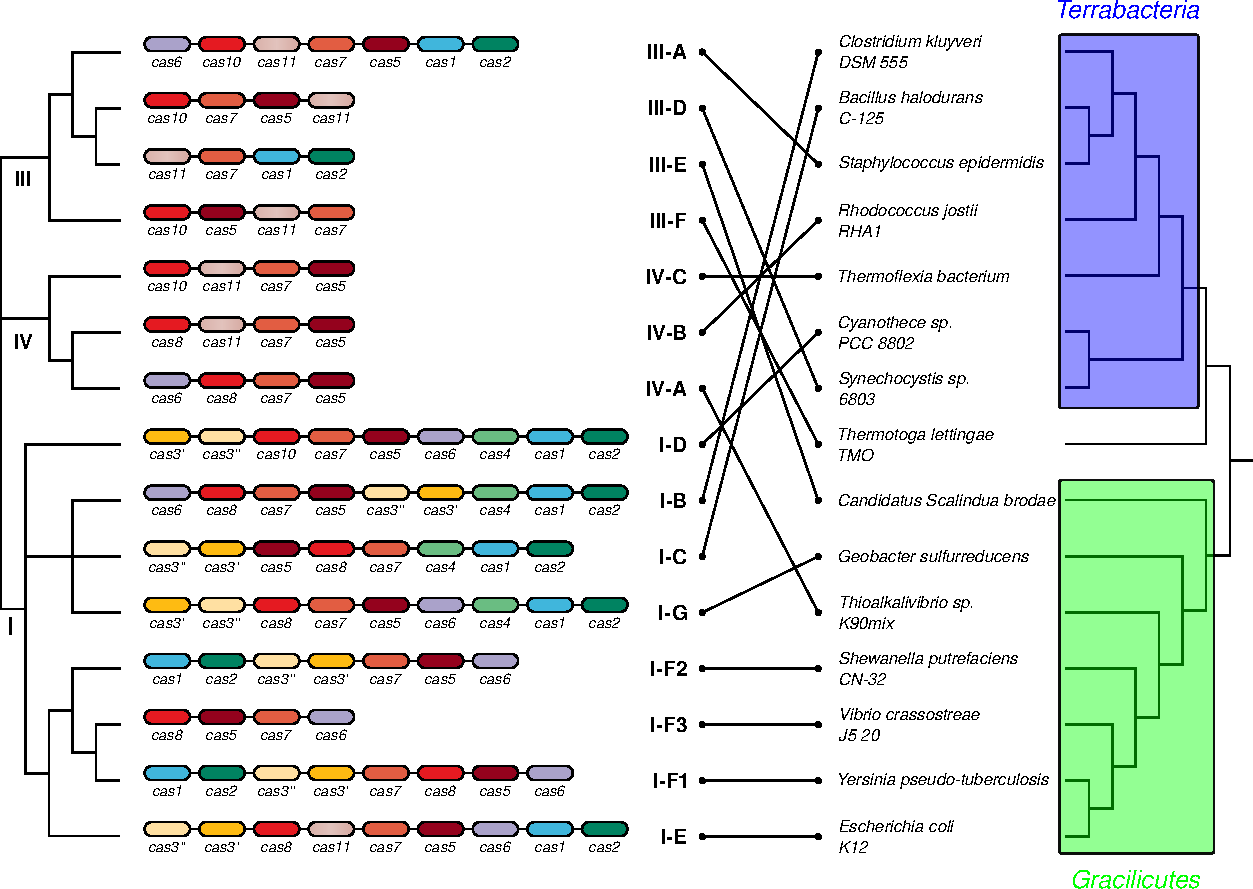
\includegraphics[width=\linewidth]{fig/superdtl/crispr-trees}
    \caption[Dataset of CRISPR-Cas syntenies and their host species]{
        Cas gene syntenies for the 15 considered bacterial species.
        \emph{(Left.)} Phylogeny of Class 1 CRISPR-Cas systems with subtypes names, as presented by~\textcite{Makarova2020EvolutionaryClassificationCRISPR} with our preprocessing of syntenies as described in the text.
        \emph{(Right.)} The species tree based on the topology inferred by~\textcite{Coleman2021RootedPhylogenyResolves} with representation of the two major groups of bacteria, Terrabacteria and Gracilicutes.
        Lines represent the correspondence between the Cas genes syntenies and the species they belong to, illustrating the high incongruence between the topology of the synteny tree and that of the species tree.
        \label{fig:superdtl:crispr-trees}
    }
\end{figure}

We repurposed the phylogenetic tree given in figure~1 of \textcite{Makarova2020EvolutionaryClassificationCRISPR} as our synteny tree.
Some alterations of the syntenies were required to fit the constraints of the model. We considered Cas families Cas1--8 and Cas10--11. Since a part of Cas3, Cas3", can work as a standalone HD nuclease, we split Cas3 into Cas3' and Cas3".
In the paper by~\textcite{Makarova2020EvolutionaryClassificationCRISPR}, Cas10 and Cas8 share the same colour code as they provide similar functions in CRISPR-Cas complexes. Indeed, it was initially believed that Cas8 evolved from Cas10~\parencite{Makarova2011UnificationCasProtein}. Nevertheless, their sequence being extremely divergent, we decided to consider them as not homologous and to conserve separate Cas8 and Cas10 families. Finally, for syntenies with several copies of the same family, we conserved only one copy per synteny. The obtained  Cas gene syntenies are illustrated in the left part of \cref{fig:superdtl:crispr-trees}.

\section{Results}\label{sec:superdtl:results}

\subsection{DTL super-reconciliation settings}

We used {\superdtl} to predict optimal DTL Super-reconciliations for the syntenies and trees depicted in \cref{fig:superdtl:crispr-trees}. Notice that the synteny tree is non-binary and contains three multifurcations, one at the root and two in the subtree of Type I CRISPR-Cas systems. As our algorithm can only be applied to binary trees, we test all possible \enquote{binarizations} of the synteny tree and retain the overall minimal solutions.

We tested different values for the $\delta = \tuple{\costDup, \costHGT, \costLoss}$ cost model, in agreement with a classical assumption that HGTs are less frequent than duplications, which are less frequent than losses. The number of solutions obtained for each setting is given in \cref{tab:superdtl:sol-count}. We observe that the number of solutions decreases as the HGT cost increases, reaching a minimum for $\costHGT=4$, and then increases again. For a given $\costHGT$, the results are largely stable for different $\costDup$ values.

\begin{table}[h]
    \capstart
    \centering
    \setlength{\tabcolsep}{8pt}
    \begin{tabular}{cccccc}
    \toprule
     {\bf $\costHGT$\textbackslash$\costDup$} & {\bf 1} & {\bf 1.5} & {\bf 2} & {\bf 2.5} & {\bf 3}\\
    \midrule
    1 & 1376 & 1376 & 1376 & 1376 & 1376 \\ \midrule
    2 & 132 & 132 & 132 & 132 & 132 \\ \midrule
    3 & 112 & 60 & 60 & 60 & 60 \\ \midrule
    4 & 32 & 32 & 32 & 32 & 48 \\ \midrule
    5 & 288 & 288 & 320 & 32 & 32 \\ \midrule
    6 & 320 & 288 & 288 & 288 & 288 \\
    \bottomrule
    \end{tabular}
    \caption[Number of SuperDTL solutions for various cost settings]{
        Number of solutions obtained by Algorithm {\superdtl} for different values of $\delta = \tuple{\costDup, \costHGT, \costLoss}$, with $\costLoss = 1$.
        \label{tab:superdtl:sol-count}
    }
\end{table}

\begin{figure}[htbp]
    \capstart
    \centering%
    \scalebox{.66}{\colorlet{species background color}{black!10}%
\tikzset{
    x={.95pt},
    y={-1pt},
    species background/.style={
        fill=species background color,
        draw=species background color,
        line width={1pt},
    },
    species label/.style={
        midway,
        anchor=west,
        align=left,
        xshift=5,
    },
    branch/.style={
        draw={#1},
        line width={0.5pt},
    },
    transfer branch/.style={
        branch={#1},
        -Stealth,
    },
    loss/.style={
        draw={#1}, cross out, thick,
        line width={0.5pt},
        inner sep=0pt,
        outer sep=0pt,
        minimum width={3},
        minimum height={3},
    },
    extant gene/.style 2 args={
        circle, fill={#1},
        outer sep=0pt, inner sep=0pt,
        minimum size={3},
        label={
            [font={\color{#1}},
                align=justify,
                inner xsep=4pt, inner ysep=0pt,
                outer xsep=0pt, outer ysep=0pt]
            right:#2
        },
    },
    extant gene/.default={black}{},
    branch node/.style={
        draw={#1}, fill={species background color!50!white},
        align=center,
        font={\color{#1}},
        outer sep=0pt, inner xsep=0pt, inner ysep=2pt,
        line width={0.5pt},
    },
    branch node/.default={black},
    speciation/.style={
        branch node={#1}, rectangle, rounded corners,
        inner xsep=4pt,
        minimum width={8},
        minimum height={8},
    },
    duplication/.style={
        branch node={#1}, rectangle,
        inner xsep=4pt,
        minimum width={8},
        minimum height={8},
    },
    horizontal gene transfer/.style={
        branch node={#1}, chamfered rectangle,
        chamfered rectangle sep={8 / 2.4},
        inner xsep=2pt,
        inner ysep=-1pt,
        minimum width={8},
        minimum height={8},
    },
    gain/.style 2 args={
        branch node={#1}, circle, inner sep=1.5pt,
        label={[font={\strut\scriptsize},xshift=-2pt]right:\color{#1}#2},
    },
    type label/.style 2 args={
        rectangle,
        fill=#1,
        inner sep=0pt,
        outer sep=0pt,
        minimum width=1pt,
        minimum height=6pt,
        label={above:\color{#1}#2},
    },
    group brace/.style={
        decorate,
        decoration={brace},
    },
    group label/.style={
        right=12pt,
        rotate=-90,
        anchor=center,
    },
    clade brace/.style={
        group brace,
        very thick,
    },
    clade label/.style={
        group label,
        font=\bfseries,
    },
}%
\definecolor{reccolor0}{HTML}{000000}%
\definecolor{reccolor1}{HTML}{DB0505}%
\definecolor{reccolor2}{HTML}{0037DB}%
\definecolor{reccolor3}{HTML}{0C8F00}%
\begin{tikzpicture}
% background
\path[species background] (42.17000999999999,269.52636) [rounded corners={4pt}] -- (10,269.52636) -- (10,298.21633) [sharp corners] -- (0,298.21633) -- (0,298.21633) [rounded corners={4pt}] -- (10,298.21633) -- (10,326.90630000000004) [sharp corners] -- (14.0,326.90630000000004) -- (14.0,326.90630000000004) [rounded corners={4pt}] -- (10,326.90630000000004) -- (10,269.52636) [sharp corners] -- (42.17000999999999,269.52636) -- cycle;
\path[species background] (56.17000999999999,163.114845) [rounded corners={4pt}] -- (52.17000999999999,163.114845) -- (52.17000999999999,269.52636) [sharp corners] -- (42.17000999999999,269.52636) -- (42.17000999999999,269.52636) [rounded corners={4pt}] -- (52.17000999999999,269.52636) -- (52.17000999999999,292.21633) [sharp corners] -- (318.94,292.21633) -- (318.94,275.52636) [rounded corners={4pt}] -- (52.17000999999999,275.52636) -- (52.17000999999999,184.30481500000002) [sharp corners] -- (56.17000999999999,184.30481500000002) -- cycle;
\path[species background] (157.22,136.76986) [rounded corners={4pt}] -- (66.17000999999999,136.76986) -- (66.17000999999999,163.114845) [sharp corners] -- (56.17000999999999,163.114845) -- (56.17000999999999,184.30481500000002) [rounded corners={4pt}] -- (66.17000999999999,184.30481500000002) -- (66.17000999999999,246.83639) [sharp corners] -- (158.83341,246.83639) -- (158.83341,213.74642) [rounded corners={4pt}] -- (153.21999999999997,213.74642) -- (153.21999999999997,153.26986) [sharp corners] -- (157.22,153.26986) -- cycle;
\path[species background] (187.72,110.57989) [rounded corners={4pt}] -- (167.22,110.57989) -- (167.22,136.76986) [sharp corners] -- (157.22,136.76986) -- (157.22,153.26986) [rounded corners={4pt}] -- (167.22,153.26986) -- (167.22,167.70983) [sharp corners] -- (318.94,167.70983) -- (318.94,151.01986) [rounded corners={4pt}] -- (183.72,151.01986) -- (183.72,122.07989) [sharp corners] -- (187.72,122.07989) -- cycle;
\path[species background] (213.22,18.18498) [rounded corners={4pt}] -- (197.72,18.18498) -- (197.72,110.57989) [sharp corners] -- (187.72,110.57989) -- (187.72,122.07989) [rounded corners={4pt}] -- (197.72,122.07989) -- (197.72,139.01986) [sharp corners] -- (309.43991,139.01986) -- (309.43991,122.32989) [rounded corners={4pt}] -- (209.22,122.32989) -- (209.22,51.55494) [sharp corners] -- (213.22,51.55494) -- cycle;
\path[species background] (317.82999,0) [rounded corners={4pt}] -- (223.22,0) -- (223.22,18.18498) [sharp corners] -- (213.22,18.18498) -- (213.22,51.55494) [rounded corners={4pt}] -- (223.22,51.55494) -- (223.22,81.48992) [sharp corners] -- (293.15999999999997,81.48992) -- (293.15999999999997,69.98992) [rounded corners={4pt}] -- (289.15999999999997,69.98992) -- (289.15999999999997,28.86996) [sharp corners] -- (317.82999,28.86996) -- cycle;
\path[
                species background,
                rounded corners={4pt},
            ] (317.82999,0) -- (389.26999,0) -- node[species label] (terra-start) {Clostridium\\kluyveri DSM 555} (389.26999,28.86996) -- (317.82999,28.86996);
\path[species background] (318.65999999999997,40.86996) [rounded corners={4pt}] -- (303.15999999999997,40.86996) -- (303.15999999999997,69.98992) [sharp corners] -- (293.15999999999997,69.98992) -- (293.15999999999997,81.48992) [rounded corners={4pt}] -- (303.15999999999997,81.48992) -- (303.15999999999997,110.32989) [sharp corners] -- (326.15999999999997,110.32989) -- (326.15999999999997,81.73992) [rounded corners={4pt}] -- (314.65999999999997,81.73992) -- (314.65999999999997,69.73992) [sharp corners] -- (318.65999999999997,69.73992) -- cycle;
\path[
                species background,
                rounded corners={4pt},
            ] (318.65999999999997,40.86996) -- (389.26999,40.86996) -- node[species label] {Bacillus\\halodurans C-125} (389.26999,69.73992) -- (318.65999999999997,69.73992);
\path[
                species background,
                rounded corners={4pt},
            ] (326.15999999999997,81.73992) -- (389.26998999999995,81.73992) -- node[species label] (firmi-end) {Staphylococcus\\epidermidis} (389.26998999999995,110.32989) -- (326.15999999999997,110.32989);
\path[
                species background,
                rounded corners={4pt},
            ] (309.43991,122.32989) -- (389.26999,122.32989) -- node[species label] {Rhodococcus\\jostii RHA1} (389.26999,139.01986) -- (309.43991,139.01986);
\path[
                species background,
                rounded corners={4pt},
            ] (318.94,151.01986) -- (389.26999,151.01986) -- node[species label] {Thermoflexia\\bacterium} (389.26999,167.70983) -- (318.94,167.70983);
\path[species background] (237.6634,179.70983) [rounded corners={4pt}] -- (168.83341,179.70983) -- (168.83341,213.74642) [sharp corners] -- (158.83341,213.74642) -- (158.83341,246.83639) [rounded corners={4pt}] -- (168.83341,246.83639) -- (168.83341,263.52636) [sharp corners] -- (275.43973,263.52636) -- (275.43973,246.83639000000002) [rounded corners={4pt}] -- (233.6634,246.83639000000002) -- (233.6634,213.74642) [sharp corners] -- (237.6634,213.74642) -- cycle;
\path[
                species background,
                rounded corners={4pt},
            ] (237.6634,179.70983) -- (389.26999,179.70983) -- node[species label] (cyano-start) {Cyanothece\\sp. PCC 8802} (389.26999,213.74642) -- (237.6634,213.74642);
\path[
                species background,
                rounded corners={4pt},
            ] (275.43973,246.83639000000002) -- (389.26999,246.83639000000002) -- node[species label] (terra-end) {Synechocystis\\sp. 6803} (389.26999,263.52636) -- (275.43973,263.52636);
\path[
                species background,
                rounded corners={4pt},
            ] (318.94,275.52636) -- (389.26999,275.52636) -- node[species label] {Thermotoga\\lettingae TMO} (389.26999,292.21633) -- (318.94,292.21633);
\path[species background] (323.94,304.21633) [rounded corners={4pt}] -- (24.0,304.21633) -- (24.0,326.90630000000004) [sharp corners] -- (14.0,326.90630000000004) -- (14.0,326.90630000000004) [rounded corners={4pt}] -- (24.0,326.90630000000004) -- (24.0,386.676235) [sharp corners] -- (28.0,386.676235) -- (28.0,353.306275) [rounded corners={4pt}] -- (24.0,353.306275) -- (24.0,320.90630000000004) [sharp corners] -- (323.94,320.90630000000004) -- cycle;
\path[
                species background,
                rounded corners={4pt},
            ] (323.94,304.21633) -- (389.26999,304.21633) -- node[species label] (gracil-start) {Candidatus\\Scalindua brodae} (389.26999,320.90630000000004) -- (323.94,320.90630000000004);
\path[species background] (303.3299,332.90630000000004) [rounded corners={4pt}] -- (38.0,332.90630000000004) -- (38.0,353.306275) [sharp corners] -- (28.0,353.306275) -- (28.0,386.676235) [rounded corners={4pt}] -- (38.0,386.676235) -- (38.0,406.6462200000001) [sharp corners] -- (118.22000000000003,406.6462200000001) -- (118.22000000000003,395.1462200000001) [rounded corners={4pt}] -- (114.22,395.1462200000001) -- (114.22,361.77626000000004) [sharp corners] -- (303.3299,361.77626000000004) -- cycle;
\path[
                species background,
                rounded corners={4pt},
            ] (303.3299,332.90630000000004) -- (389.26999,332.90630000000004) -- node[species label] (proteo-start) {Geobacter\\sulfurreducens} (389.26999,361.77626000000004) -- (303.3299,361.77626000000004);
\path[species background] (328.94,378.20625000000007) [rounded corners={4pt}] -- (128.22000000000003,378.20625000000007) -- (128.22000000000003,395.1462200000001) [sharp corners] -- (118.22000000000003,395.1462200000001) -- (118.22000000000003,406.6462200000001) [rounded corners={4pt}] -- (128.22000000000003,406.6462200000001) -- (128.22000000000003,472.54115500000006) [sharp corners] -- (143.72,472.54115500000006) -- (143.72,430.67119500000007) [rounded corners={4pt}] -- (139.72000000000003,430.67119500000007) -- (139.72000000000003,394.8962200000001) [sharp corners] -- (328.94,394.8962200000001) -- cycle;
\path[
                species background,
                rounded corners={4pt},
            ] (328.94,378.20625000000007) -- (389.26999,378.20625000000007) -- node[species label] {Thioalkalivibrio\\sp. K90mix} (389.26999,394.8962200000001) -- (328.94,394.8962200000001);
\path[species background] (324.22,406.8962200000001) [rounded corners={4pt}] -- (162.22,406.8962200000001) -- (162.22,430.67119500000007) [sharp corners] -- (143.72,430.67119500000007) -- (143.72,472.54115500000006) [rounded corners={4pt}] -- (162.22,472.54115500000006) -- (162.22,502.63614000000007) [sharp corners] -- (239.82999,502.63614000000007) -- (239.82999,477.63614000000007) [rounded corners={4pt}] -- (235.82999,477.63614000000007) -- (235.82999,435.7661800000001) [sharp corners] -- (324.22,435.7661800000001) -- cycle;
\path[
                species background,
                rounded corners={4pt},
            ] (324.22,406.8962200000001) -- (389.26999,406.8962200000001) -- node[species label] {Shewanella\\putrefaciens CN-32} (389.26999,435.7661800000001) -- (324.22,435.7661800000001);
\path[species background] (328.94,467.44617000000005) [rounded corners={4pt}] -- (249.82999,467.44617000000005) -- (249.82999,477.63614000000007) [sharp corners] -- (239.82999,477.63614000000007) -- (239.82999,502.63614000000007) [rounded corners={4pt}] -- (249.82999,502.63614000000007) -- (249.82999,545.0061000000001) [sharp corners] -- (278.82999,545.0061000000001) -- (278.82999,525.0061000000001) [rounded corners={4pt}] -- (274.82999,525.0061000000001) -- (274.82999,484.13614000000007) [sharp corners] -- (328.94,484.13614000000007) -- cycle;
\path[
                species background,
                rounded corners={4pt},
            ] (328.94,467.44617000000005) -- (389.26999,467.44617000000005) -- node[species label] {Vibrio\\crassostreae J5 20} (389.26999,484.13614000000007) -- (328.94,484.13614000000007);
\path[species background] (318.65999999999997,496.13614000000007) [rounded corners={4pt}] -- (288.82999,496.13614000000007) -- (288.82999,525.0061000000001) [sharp corners] -- (278.82999,525.0061000000001) -- (278.82999,545.0061000000001) [rounded corners={4pt}] -- (288.82999,545.0061000000001) -- (288.82999,573.87606) [sharp corners] -- (312.82999,573.87606) -- (312.82999,545.0061000000001) [rounded corners={4pt}] -- (308.82999,545.0061000000001) -- (308.82999,525.0061000000001) [sharp corners] -- (318.65999999999997,525.0061000000001) -- cycle;
\path[
                species background,
                rounded corners={4pt},
            ] (318.65999999999997,496.13614000000007) -- (389.26999,496.13614000000007) -- node[species label] {Yersinia\\pseudotuberculosis} (389.26999,525.0061000000001) -- (318.65999999999997,525.0061000000001);
\path[
                species background,
                rounded corners={4pt},
            ] (312.82999,545.0061000000001) -- (389.26999,545.0061000000001) -- node[species label] (gracil-end) {Escherichia coli K12} (389.26999,573.87606) -- (312.82999,573.87606);
% clade names
\coordinate (group-labels) at (490,0);
\draw[group brace] (group-labels|-terra-start.north) -- node[group label] {Firmicutes} (group-labels|-firmi-end.south);
\draw[group brace] (group-labels|-cyano-start.north) -- node[group label] {Cyanobacteria} (group-labels|-terra-end.south);
\draw[group brace] (group-labels|-proteo-start.north) -- node[group label] {Proteobacteria} (group-labels|-gracil-end.south);
\coordinate (clade-labels) at (515,0);
\draw[clade brace] (clade-labels|-terra-start.north) -- node[clade label] {Terrabacteria} (clade-labels|-terra-end.south);
\draw[clade brace] (clade-labels|-gracil-start.north) -- node[clade label] {Gracilicutes} (clade-labels|-gracil-end.south);
% gene branches
\path[branch={reccolor0}] (70.17000999999999,173.70983) -- (56.17000999999999,173.70983);
\draw[branch={reccolor0}] (137.22,145.01986) -| (109.69500499999998,167.114845) (109.69500499999998,180.304815) |- node[pos=.25, gain={reccolor0}{1, 2}] {} (158.83341,230.291405);
\path[branch={reccolor1}] (171.22,145.01986) -- (137.22,145.01986) node[type label={reccolor1}{IV}] {};
\draw[branch={reccolor1}] (187.72,116.32989) -| (175.47,140.76986) (175.47,149.26986) |- (318.94,159.364845);
\path[branch={reccolor1}] (203.47,116.32989) -- (187.72,116.32989);
\draw[branch={reccolor1}] (203.47,116.32989) -- (203.47,110.57989);
\draw[branch={reccolor1}] (203.47,116.32989) |- (309.43991,130.674875);
\path[branch={reccolor2}] (227.22,34.869960000000006) -- (213.22,34.869960000000006);
\draw[branch={reccolor2}] (317.82999,14.43498) -| (256.19,22.184980000000003) (256.19,47.55494) |- (293.15999999999997,75.73992);
\path[branch={reccolor2}] (327.82999,14.43498) -- (317.82999,14.43498);
\path[branch={reccolor2}] (308.90999999999997,75.73992) -- (293.15999999999997,75.73992);
\draw[branch={reccolor2}] (308.90999999999997,75.73992) -- (308.90999999999997,81.48992);
\draw[branch={reccolor2}] (308.90999999999997,75.73992) |- (318.65999999999997,55.30494);
\path[branch={reccolor2}] (328.66,55.30494) -- (318.65999999999997,55.30494);
\path[branch={reccolor3}] (336.15999999999997,96.03490500000001) -- (326.15999999999997,96.03490500000001);
\path[branch={reccolor1}] (319.43991,130.674875) -- (309.43991,130.674875);
\draw[branch={reccolor1}] (333.94,130.674875) |- (329.94,130.674875);
\path[branch={reccolor1}] (328.94,159.36484500000003) -- (318.94,159.364845);
\path[branch={reccolor0}] (172.83341,230.291405) -- (158.83341,230.291405);
\draw[branch={reccolor0}] (222.6634,196.728125) -| node[pos=.75, gain={reccolor0}{3', 3", 4}] {} (201.248405,217.74642) (201.248405,242.83639) |- (250.43973,255.181375);
\path[branch={reccolor2}] (247.6634,196.728125) -- (222.6634,196.728125) node[type label={reccolor2}{I}] {};
\draw[branch={reccolor2}] (333.38001,196.728125) |- (329.38000999999997,196.728125);
\draw[branch={reccolor3}] (328.94,255.18137500000003) |- (324.94,255.181375);
\draw[branch={reccolor3}] (314.43991,255.181375) |- (285.43991,255.181375);
\path[branch={reccolor3}] (285.43973,255.181375) -- (250.43973,255.181375) node[type label={reccolor3}{III}] {};
\draw[branch={reccolor3}] (299.93982,255.181375) |- (295.93982,255.181375);
\path[branch={reccolor3}] (328.94,283.871345) -- (276.689775,283.871345);
\path[branch={reccolor3}] (333.94,312.56131500000004) -- (319.689955,312.56131500000004);
\path[branch={reccolor2}] (42.0,369.991255) -- (28.0,369.991255);
\draw[branch={reccolor2}] (303.3299,347.34128000000004) -| (76.11,357.306275) (76.11,382.676235) |- (118.22000000000003,400.8962200000001);
\path[branch={reccolor2}] (313.3299,347.34128000000004) -- (303.3299,347.34128000000004);
\draw[branch={reccolor2}] (327.82999,347.34128000000004) |- (313.3299,347.34128000000004);
\path[branch={reccolor2}] (133.97000000000003,400.8962200000001) -- (118.22000000000003,400.8962200000001);
\draw[branch={reccolor2}] (133.97000000000003,400.8962200000001) -- (133.97000000000003,395.1462200000001);
\draw[branch={reccolor2}] (133.97000000000003,400.8962200000001) |- (143.72,446.13868500000007);
\path[branch={reccolor1}] (338.94,386.5512350000001) -- (328.94,386.5512350000001);
\draw[branch={reccolor2}] (324.22,421.3312000000001) -| (194.774995,443.17119500000007) (194.774995,468.54115500000006) |- (239.82999,494.38614000000007);
\draw[branch={reccolor2}] (230.07999,436.42119500000007) -- (230.07999,430.67119500000007);
\draw[branch={reccolor2}] (230.07999,436.42119500000007) |- (239.82999,483.38614000000007);
\path[branch={reccolor2}] (153.72,446.13868500000007) -- (143.72,446.13868500000007);
\draw[branch={reccolor2}] (230.07999,436.42119500000007) -| (157.97,441.88868500000007) (157.97,450.38868500000007) |- (166.22,455.85617500000006);
\path[branch={reccolor2}] (334.22,421.3312000000001) -- (324.22,421.3312000000001);
\path[branch={reccolor2}] (253.82999,494.38614000000007) -- (239.82999,494.38614000000007);
\draw[branch={reccolor2}] (328.94,475.79115500000006) -| (258.07999,490.13614000000007) (258.07999,498.63614000000007) |- (278.82999,539.2561000000001);
\path[branch={reccolor2}] (269.07999,483.38614000000007) -- (239.82999,483.38614000000007);
\draw[branch={reccolor2}] (269.07999,483.38614000000007) -- (269.07999,480.63614000000007);
\draw[branch={reccolor2}] (269.07999,483.38614000000007) |- (278.82999,530.7561000000001);
\path[branch={reccolor2}] (338.94,475.79115500000006) -- (328.94,475.79115500000006);
\path[branch={reccolor2}] (294.57999,539.2561000000001) -- (278.82999,539.2561000000001);
\draw[branch={reccolor2}] (294.57999,539.2561000000001) -- (294.57999,545.0061000000001);
\draw[branch={reccolor2}] (294.57999,539.2561000000001) |- (318.65999999999997,510.57112000000006);
\path[branch={reccolor2}] (303.07999,530.7561000000001) -- (278.82999,530.7561000000001);
\draw[branch={reccolor2}] (303.07999,530.7561000000001) -- (303.07999,525.0061000000001);
\draw[branch={reccolor2}] (303.07999,530.7561000000001) |- (312.82999,559.44108);
\path[branch={reccolor2}] (328.66,510.57112000000006) -- (318.65999999999997,510.57112000000006);
\path[branch={reccolor2}] (322.82999,559.44108) -- (312.82999,559.44108);
% gene transfers
\draw[transfer branch={reccolor1}] (324.689955,130.67) to[bend right] (328.94,386.5512350000001);
\draw[transfer branch={reccolor2}] (273.521705,209.74642) to[out distance=160pt, out=-90, in=70] (28.0,369.991255);
\draw[transfer branch={reccolor3}] (319.689955,259.431375) to[out=-90, in=90] (319.689955,312.56131500000004);
\draw[transfer branch={reccolor3}] (305.189865,250.931375) to[out=90, in=-110] (326.15999999999997,96.03490500000001);
\draw[transfer branch={reccolor3}] (276.689775,259.431375) to (276.689775,283.871345);
\draw[transfer branch={reccolor2}] (213.579945,347.34) to[bend left=18] (213.22,34.869960000000006);
% events
\node[speciation={reccolor0}] at (109.69500499999998,173.70983) {5, 6, 7, 8, 10, 11};
\node[speciation={reccolor1}] at (175.47,145.01986) {};
\node[loss={reccolor1}] at (203.47,110.57989) {};
\node[speciation={reccolor2}] at (256.19,34.869960000000006) {1, 2, 3', 3",\\4, 5, 6, 7, 8};
\node[extant gene={reccolor2}{1, 2, 3', 3",\\4, 5, 6, 7, 8}] at (329.32999,14.43498) {};
\node[loss={reccolor2}] at (308.90999999999997,81.48992) {};
\node[extant gene={reccolor2}{1, 2, 3', 3",\\4, 5, 7, 8}] at (330.16,55.30494) {};
\node[extant gene={reccolor3}{1, 2, 5, 6,\\7, 10, 11}] at (337.65999999999997,96.03490500000001) {};
\node[extant gene={reccolor1}{5, 7, 8, 11}] at (335.44,130.674875) {};
\node[horizontal gene transfer={reccolor1}] at (324.689955,130.674875) {\phantom{-}};
\node[extant gene={reccolor1}{5, 7, 10, 11}] at (330.44,159.36484500000003) {};
\node[speciation={reccolor0}] at (201.248405,230.291405) {1, 2, 5, 6,\\7, 8, 10, 11};
\node[extant gene={reccolor2}{1, 2, 3', 4,\\5, 6, 7, 10}] at (334.88001,196.728125) {};
\node[horizontal gene transfer={reccolor2}] at (288.521705,196.728125) {1, 2, 3', 3", 4,\\5, 6, 7, 8, 10, 11};
\node[extant gene={reccolor3}{5, 7, 10, 11}] at (330.44,255.18137500000003) {};
\node[horizontal gene transfer={reccolor3}] at (319.689955,255.181375) {\phantom{-}};
\node[horizontal gene transfer={reccolor3}] at (305.189865,255.181375) {\phantom{-}};
\node[horizontal gene transfer={reccolor3}] at (276.689775,255.181375) {\phantom{-}};
\node[extant gene={reccolor3}{5, 7, 10, 11}] at (330.44,283.871345) {};
\node[extant gene={reccolor3}{1, 2, 7, 11}] at (335.44,312.56131500000004) {};
\node[speciation={reccolor2}] at (76.11,369.991255) {1, 2, 3', 3", 4,\\5, 6, 7, 8, 11};
\node[extant gene={reccolor2}{1, 2, 3', 3",\\4, 5, 6, 7, 8}] at (329.32999,347.34128000000004) {};
\node[horizontal gene transfer={reccolor2}] at (213.579945,347.34128000000004) {\phantom{-}};
\node[loss={reccolor2}] at (133.97000000000003,395.1462200000001) {};
\node[extant gene={reccolor1}{5, 6, 7, 8}] at (340.44,386.5512350000001) {};
\node[speciation={reccolor2}] at (194.774995,455.85617500000006) {1, 2, 3', 3",\\5, 6, 7, 8};
\node[loss={reccolor2}] at (230.07999,430.67119500000007) {};
\node[duplication={reccolor2}] at (157.97,446.13868500000007) {};
\node[extant gene={reccolor2}{1, 2, 3',\\3", 5, 6, 7}] at (335.72,421.3312000000001) {};
\node[speciation={reccolor2}] at (258.07999,494.38614000000007) {};
\node[loss={reccolor2}] at (269.07999,480.63614000000007) {};
\node[extant gene={reccolor2}{5, 6, 7, 8}] at (340.44,475.79115500000006) {};
\node[loss={reccolor2}] at (294.57999,545.0061000000001) {};
\node[loss={reccolor2}] at (303.07999,525.0061000000001) {};
\node[extant gene={reccolor2}{1, 2, 3', 3",\\5, 6, 7, 8}] at (330.16,510.57112000000006) {};
\node[extant gene={reccolor2}{1, 2, 3', 3",\\5, 6, 7, 8, 11}] at (324.32999,559.44108) {};
\end{tikzpicture}%}%
    \caption[Most parsimonious scenario for the CRISPR-Cas dataset under SuperDTL]{
        Representation of one of the 32 solutions inferred by Algorithm {\superdtl} reconstructing a DTL evolutionary history of the Class~1 Cas gene synteny dataset illustrated in \cref{fig:superdtl:crispr-trees}.
        Event costs set to $\costLoss=1$, $\costHGT=4$ and $\costDup\in\{1,1.5,2,2.5\}$ yield equal solutions.
        The red, blue, and green parts of the tree reflect the evolution of Cas synteny types IV, I, and III respectively.
        Gains of Cas1+Cas2 and Cas3(Cas3'+Cas3")+Cas4 are illustrated.
        \label{fig:superdtl:crispr-scenario}
    }
\end{figure}

\subsection{An evolutionary scenario}

We analyzed the 32 solutions generated for $\costHGT=4$ and $\costDup\in\{1,1.5,2,2.5\}$. All solutions lead to the same resolution of the three multifurcations in the synteny tree, and the incongruence observed between the species and synteny tree topologies is mainly resolved by inferring six HGTs and one duplication. The 32 solutions only differ from one another by minor variations, such as gene losses located either before or after a speciation or HGT event, which do not change the overall inferred evolutionary history for the Cas gene syntenies.

\Cref{fig:superdtl:crispr-scenario} is a representation of one of these solutions. The evolutionary reconstruction is broadly consistent with the CRISPR-Cas evolution scenario established by \textcite{Koonin2022EvolutionaryPlasticityFunctional}. In both their scenario and ours, the CRISPR-Cas systems emerge from an initial adaptive immune system composed only of Cas genes involved in the effector complex (Cas5--8 and Cas10--11). We see from \cref{fig:superdtl:crispr-scenario} that the CRISPR-Cas emergence is inferred at the root of Terrabacteria. The scenarios diverge on the fact that, in our scenario, Type IV emerges directly from this ancestral adaptive immune system before the acquisition of Cas1 and Cas2 genes, while in \citeauthor{Koonin2022EvolutionaryPlasticityFunctional}'s scenario, Type IV emerges after the acquisition of Cas1 and Cas2 adaptation module genes and loss of several Cas genes.
Aside from this difference, both scenarios are in agreement for Types I and III in terms of gene content in ancestral Cas syntenies. As it appears in \cref{fig:superdtl:crispr-scenario}, Types I and III Cas syntenies emerge from Cyanobacteria after the acquisition of Cas1 and Cas2 by an ancestor of Cyanobacteria. Type I emerges from the branch leading to \emph{Cyanothece sp. PCC 8802} with acquisition of Cas3 and Cas4, while Type III emerges from the branch leading to \emph{Synechocystis sp. 6803} without further gene gains.

Type I was spread to the other bacteria with a HGT to the ancestor of Proteobacteria. According to \textcite{Wang2020EvolutionaryTimelineGenomic}, the Cyanobacteria ancestor is estimated between 2,230 and 3,000 Mya, while the last common ancestor (LCA) of Alpha-, Beta-, and Gammaproteobacteria is estimated between 2,360 and 2,620 Mya. These calibrations make time-plausible the lateral transfer of Type I CRISPR-Cas from the \emph{Cyanothece sp. PCC 8802} branch, close to the Cyanobacteria ancestor, to the LCA of Proteobacteria. A second HGT from \emph{Geobacter sulfurreducens} brought Type I to the Firmicutes \emph{Bacillus halodurans C-125} and \emph{Clostridium kluyveri DSM 555}. Type III was spread across bacteria with a succession of three HGTs, which also seem time-consistent.

The analysis of the synteny evolutionary history across the Proteobacteria subtree shows an unexpected scenario highlighting a limitation of our model. The {\superdtl} algorithm inferred an ancestral synteny duplication before the LCA of \emph{S. putrefaciens}, \emph{V. crassostreae}, \emph{Y. pseudotuberculosis} and \emph{E. coli} resulting in a succession of three consecutive full synteny losses along the branch to the synteny in \emph{E. coli} which is an unlikely evolutionary scenario. An alternative evolutionary scenario would consist in a speciation in place of the duplication, copying the ancestral synteny to an unsampled or extinct species which would later be transferred back to \emph{Escherichia coli}. Such a model of HGT events as combinations of a speciation event outside the species tree (to an unsampled or dead lineage) followed by a transfer back inside the species tree has been described in~\textcite{Szoelloesi2013LateralGeneTransfer}.
This alternative scenario would replace one duplication and three losses with one speciation and one transfer, which yields the same cost under the $\costLoss=1$, $\costHGT=4$ and $\costDup\in\{1,1.5,2,2.5\}$ model but would be less costly for $\costHGT<4$. Consideration of unsampled and dead lineages in the DTL Super-reconciliation will therefore be necessary to infer better synteny evolutionary scenarios.

\section{Conclusion}

We have developed {\superdtl}, the first exact algorithm for inferring most parsimonious evolutionary histories for a set of syntenies, given a phylogenetic tree of the syntenies and a phylogenetic tree of the corresponding species, for an evolutionary model accounting for segmental duplications, gains, losses and HGT events. We only presented the unordered version of the problem in this paper, but the algorithm developed by~\textcite{Delabre2020EvolutionSegmentalDuplications} for the ordered version of the DL Super-reconciliation model can also be extended to the DTL Super-reconciliation model. However, as rearrangements are not considered in the model, a DT or DTL Super-reconciliation only exists if extant gene orders are pairwise consistent, which is a strong constraint, not verified, for example, in the case of the Cas gene syntenies of \cref{fig:superdtl:crispr-trees}. Considering a unifying model accounting for both DTL and rearrangement events remains a challenge. The analysis of the synteny evolutionary scenario in Proteobacteria emphasized the need in DTL Super-reconciliation model to infer HGT to and from unsampled or extinct species to produce more realistic evolutionary scenarios.
In addition, in order to avoid the unjustified constraint of having all genes at the root of the tree, we allowed for gene gains, which has been essential for the analysis of Cas gene syntenies. Although we defined the general evolutionary model in a way allowing for segmental gains (i.e. gains of a group of genes), we only considered single gene gains in our algorithm. An extension is however possible and may be considered for future work.

The reconstruction of an evolutionary history for Cas gene syntenies  using {\superdtl} provides a first attempt to reconcile the evolutionary scenario of Cas syntenies in the context of the evolution of bacterial species. However, several improvements could be brought to the considered Cas synteny dataset to better reconstruct its evolutionary history. First, we excluded archaea from our dataset while several studies show evidence for an emergence of CRISPR-Cas systems from archaeal species followed by horizontal transfers to bacteria. This is supported by the fact that most considered archaea have a complete CRISPR-Cas system while only part of bacteria have one. In fact, as of the latest update from January 21, 2021 of the CRISPRCasdb database\footnote{Available at \url{https://crisprcas.i2bc.paris-saclay.fr/MainDb/StrainList}}~\parencite{Pourcel2020CRISPRCasdbSuccessorCRISPRdb}, 70.64\% of analyzed archaeal species versus 36.27\% of analyzed bacteria had a complete CRISPR-Cas system.
A phylogenetic dating approach could also be used to produce a dated phylogeny of prokaryotes and to constrain HGT events.
A larger dataset with species sampling representing the diversity of archaea and bacteria with dated phylogeny and Cas synteny tree based on synteny content and sequence divergence is required to further elucidate the evolutionary history of the CRISPR-Cas system in prokaryotes.

%! TeX root = ./main.tex
% vim: set spelllang=en,fr:
\selectlanguage{french}
\chapter{Synesth: réconciliation segmentale avec hôtes non-échantillonnés}\label{chap:synesth}

L’une des limites de la méthode proposée au chapitre précédent est qu’elle ignore les interactions possibles entre les unités étudiées et des hôtes qui ne feraient pas partie de l’échantillon choisi, par exemple s’ils appartiennent à une lignée qui s’est éteinte depuis lors.
Dans le contexte de la réconciliation avec transferts horizontaux, de telles interactions sont possibles: une unité pourrait être transférée d’un hôte \(A\), ancêtre d’un hôte échantillonné, vers un hôte \(B\) inconnu, puis à nouveau transféré vers un descendant \(C \tdesc A\).
Sous le modèle précédent, ce scénario serait interprété comme une série d’autant de spéciations et de pertes que d’hôtes ancestraux qui séparent \(A\) de \(C\), ce qui peut avoir tendance à écarter artificiellement ce type de possibilité.
Cette problématique a été étudiée par plusieurs auteurs dans le contexte de la réconciliation bilatérale, par exemple récemment par \textcite{Weiner2021ImprovedDuplicationTransfer}.
Nous verrons dans ce chapitre comment étendre le modèle pour prendre en compte cette possibilité.

Nous montrons également comment intégrer un nouveau type d’événement de \emph{scission} dans le modèle, suivant lequel une synténie se partitionne en deux synténies disjointes.
Cet événement additionnel, suggéré par Russell~\textsc{Schwartz} lors de discussions à la conférence RECOMB~2022, permet de mieux prendre en compte la réalité évolutive des synténies.

Finalement, un autre enjeu important est le besoin d’estimer des coûts pour les différents types d’événements du modèle.
En pratique, la valeur exacte des coûts a une influence importante sur la teneur des scénarios inférés, bien que les procédures d’estimation de ces coûts pourraient avoir une certaine incertitude.
Il devient alors pertinent de qualifier précisément l’impact des variations des coûts sur les résultats.
Une possibilité coûteuse et imprécise consiste à échantillonner l’espace des coûts et à exécuter l’algorithme pour chacun des choix, une méthode qui s’apparente au \emph{grid search} en apprentissage automatique.
Une approche préférable consiste à caractériser l’espace des solutions Pareto-optimales, c’est-à-dire des solutions dont le nombre d’événements de chaque type fait qu’il existe un certain ensemble de coûts qui les rendent meilleures que les autres.
En nous appuyant sur les travaux de \textcite{LibeskindHadas2014ParetoOptimalPhylogenetic}, nous montrerons qu’il est possible de brosser efficacement le \emph{paysage} des scénarios de réconciliation segmentale pour une certaine instance, indépendamment de tout choix spécifique de coûts.
Pour ce faire, nous procéderons à une étude combinatoire de l’espace des réconciliations segmentales sous ce modèle étendu.

% TODO: Migrate notations to notations.tex

\newcommand{\ancest}{\leq}
\newcommand{\separ}{\mathrel{\|}}
% \newcommand{\rootOf}{\mathrm{r}}
% \newcommand{\parentOf}{\mathrm{p}}
% \newcommand{\treeNodes}{\mathrm{V}}
% \newcommand{\treeLeaves}{\mathrm{L}}
\newcommand{\treeInner}{\mathrm{I}}
% \newcommand{\treeEdges}{\mathrm{E}}
% \newcommand{\treeEdge}[2]{(#1,#2)}
\newcommand{\treePath}[3][]{\mathrm{P}_{#1}(#2, #3)}
% \newcommand{\treeDist}[3][]{\mathrm{D}_{#1}(#2, #3)}
% \newcommand{\LCA}{\mathrm{lca}}
\newcommand{\children}{\mathrm{ch}}
% \newcommand{\leftChild}{_\mathrm{\ell}}
% \newcommand{\rightChild}{_\mathrm{r}}
\newcommand{\Child}{_\mathrm{c}}
% \newcommand{\geneFamily}{\Gamma}
% \newcommand{\geneFamilySet}{\mathcal{F}}
\newcommand{\augS}{\speciesTree^*}
% \newcommand{\F}{{\mathcal F}}
% \newcommand{\taxa}{{\Sigma}}
% \newcommand{\speciesOf}{s}
% \newcommand{\syntenyFamily}{\mathcal{X}}
% \newcommand{\syntenyTree}{\mathcal{T}}
% \newcommand{\syntenyOf}{x}
\newcommand{\restr}[2]{#1|_{#2}}
\newcommand{\allEvents}{\mathcal{E}}
% \newcommand{\eventSpe}{\mathrm{Spe}}
% \newcommand{\eventDup}{\mathrm{Dup}}
\newcommand{\eventCut}{\mathrm{Cut}}
\newcommand{\eventTrDup}{\mathrm{TrDup}}
\newcommand{\eventTrCut}{\mathrm{TrCut}}
\newcommand{\eventTrAll}{\mathrm{Tr}}
% \newcommand{\eventLoss}{\mathrm{Loss}}
% \newcommand{\eventGain}{\mathrm{Gain}}
\newcommand{\Hist}{\mathcal{H}}
% \newcommand{\speciesTree}{S}
% \newcommand{\eventOf}{e}
\newcommand{\eventCost}{\delta}
\newcommand{\histCost}{\mathrm{c}}
\newcommand{\targetChild}{_\mathrm{t}}
\newcommand{\conservChild}{_\mathrm{k}}
\newcommand{\solSpace}{\mathbb{H}}
\newcommand{\minSolSpace}{\solSpace^{\mathrm{min}}}
\newcommand{\setNat}{\mathbb{N}}
% \newcommand{\setReal}{\mathbb{R}}
\newcommand{\eventVec}{\mathrm{ev}}
\newcommand{\paretoMin}[1]{\min{}_{#1}\,}
\newcommand{\minVecSet}{\eventVec^{\mathrm{min}}}
\newcommand{\makeNode}[1]{[#1]}
\newcommand{\optPath}{\mathrm{path}}
\newcommand{\histExt}{\preceq}
\newcommand{\gainAt}{\mathrm{gain}}
\newcommand{\syntenyMinAt}{\syntenyOf^{\mathrm{min}}}
\newcommand{\minCost}{c^{\mathrm{min}}}
\newcommand{\visLeaves}{\treeLeaves_V}

%%%%%%%%%%%%%%%%%%%%%%%

\selectlanguage{english}
\articlehat{
    \textfrench{La suite de ce chapitre est une reproduction partielle de l’article intitulé \enquote{Synesth: Comprehensive syntenic reconciliation with unsampled lineages}.
    Cet article a été écrit entre octobre~2022 et décembre~2023 et a été publié en avril~2024 dans le journal Algorithms chez MDPI.}
}
\title{Synesth: Comprehensive syntenic\\reconciliation with unsampled lineages}
\author{Mattéo Delabre \and Nadia El-Mabrouk}
\institute{Département d'informatique et de recherche opérationnelle, Université de Montréal}
\makearticlehead

\begin{abstract}
    We present Synesth, the most comprehensive and flexible tool for tree reconciliation allowing for segmental events --- involving multiple genes --- including duplications, transfers, fissions, and transient events going through unsampled species.
    We examine the combinatorial properties of this extended tree reconciliation model and study various associated optimization problems related to various granularities of the solution space.
    First, the infinite set of histories is reduced to a finite but exponential set of Pareto-optimal event histories (in terms of counts of each event type), then to a polynomial set of Pareto-optimal event vectors, eventually ending with minimum event cost histories given an event cost function. An inductive algebraic characterization of the output using a different algebra for each space granularity leads to efficient dynamic programming algorithms, ultimately ending with an \(O(mn)\) time-complexity algorithm for computing a minimum event-cost history (\(m\) and \(n\): number of nodes of the two trees).
    This time complexity matches that of the fastest algorithms for classical (i.e. without syntenies and associated events) reconciliation with transfers.
    We show how Synesth can be applied for inferring Pareto-optimal evolutionary scenarios of CRISPR-Cas systems in a set of bacterial genomes.
    An implementation of the algorithm is available at: \url{https://github.com/UdeM-LBIT/superrec2/tree/algo2024}.

    \keywords{Tree reconciliation \and Algebraic dynamic programming \and Multi-objective optimization \and Horizontal gene transfer \and Synteny \and Fission \and Unsampled lineages.}
\end{abstract}

\section{Introduction}

A \emph{gene/species trees reconciliation} is an embedding of a gene tree into a species tree explicating the topological difference between the two trees through a sequence of events shaping the gene family inside the species tree.
Gene/species tree reconciliation has been widely studied since the 80s~\parencite{Goodman1979FittingGeneLineage}, first focusing on duplication~(D) and loss~(L) events and then extending to horizontal gene transfers~(T)~\parencite{Bansal2012EfficientAlgorithmsReconciliation,Donati2015EfficientTreeReconciliation,Tofigh2011SimultaneousIdentificationDuplications} and other events such as hybridization or incomplete lineage sorting (review in~\textcite{ElMabrouk2019GeneFamilyEvolution}). One of the major drawbacks of classical reconciliation is that gene families are considered separately from one another, which is not appropriate for genes organized in \emph{syntenies}, i.e. colocalized genes likely evolving together through segmental events.

Although some work has been done to infer the evolution of adjacencies~\parencite{Duchemin2017DecostarReconstructingAncestral}, group individual events into segmental ones~\parencite{Duchemin2017PhylogenyDependenciesDependencies}, or minimize \enquote{duplication episodes}~\parencite{Dondi2019ReconcilingMultipleGenes,Paszek2018EfficientAlgorithmsGenomic}, none of these methods are intended to explicitly look for evolutionary scenarios minimizing segmental events. We presented the first algorithm generalizing reconciliation to synteny trees (i.e. with leaves representing syntenies rather than single genes) and segmental events for the DL distance in~\textcite{Delabre2020EvolutionSegmentalDuplications} and extended it to horizontal transfers with \emph{SuperDTL} in~\textcite{Anselmetti2022ReconciliationSegmentalDuplication}.

Here, we present Synesth (for \emph{SYNteny Evolution in SegmenTal Histories}), an extended reconciliation model accounting for fissions whereby part of a synteny is detached to another locus or species, in addition to losses, gains, duplications and transfers.
Moreover, as the choice of the species included in a study, or equivalently the absence of species which are not chosen, unsampled or extinct, has a serious impact on the output of a reconciliation algorithm~\parencite{Jacox2016EcceteraComprehensiveGene,Szoelloesi2013LateralGeneTransfer,Weiner2021ImprovedDuplicationTransfer}, we account for transfers going through unsampled species. 

Among the infinite space of possible histories explicating the evolution of a synteny tree inside a species tree both given as input, we are interested in selecting the most likely ones.
A possible way is by assigning costs (or probabilities) to event types and selecting histories minimizing (resp. maximizing) the overall cost (resp. probability).
The resulting histories can vary significantly depending on the costs, which are usually challenging to determine and strongly depend on the taxa under study~\parencite{LibeskindHadas2014ParetoOptimalPhylogenetic,David2011RapidEvolutionaryInnovation}.
Instead, our goal here is to provide a landscape of possible histories independently of costs, before eventually choosing a solution for a particular choice of costs.

We subdivide the space of histories by formally defining nested classes.
First, the space is reduced to a finite but exponential set of Pareto-optimal histories (in terms of counts of each event type), then to a polynomial set of Pareto-optimal vectors, eventually ending with minimum-cost solutions.
We develop efficient and exact algorithms using an algebraic dynamic programming approach with a different algebra for each class.
The inductive characterization of Pareto-optimal histories given in \cref{sec:synesth:pareto-histories} leads to a polynomial-time dynamic programming algorithm to output all Pareto-optimal vectors (\cref{sec:synesth:pareto-vectors}) and ultimately to an \(\bigo(mn)\) time-complexity algorithm (\(m\) and \(n\): number of nodes of the two trees) to output a minimum event cost history (\Cref{sec:synesth:min-cost-histories}), matching time complexity of the fastest algorithms for classical DTL reconciliation~\parencite{Weiner2021ImprovedDuplicationTransfer}.

In \cref{sec:synesth:results}, we apply Synesth to CRISPR-associated (Cas) gene syntenies.
Taking advantage of previous work~\parencite{LibeskindHadas2022TreeReconciliationMethods,LibeskindHadas2014ParetoOptimalPhylogenetic}, we output a comprehensive representation of the solution landscape comprised of \enquote{cost regions}, such that any two event cost assignments within the same region lead to the same histories.

We first introduce the required notations in \cref{sec:synesth:defs}, the evolutionary model in \cref{sec:synesth:def-model} and the solution space subdivision and considered optimization problems in \cref{sec:synesth:opt-probs}.

\section{Preliminary notation}\label{sec:synesth:defs}

% TODO: Merge with introductory notation chapter

All trees are considered rooted.
Given a tree \(T\), we denote by \(\rootOf(T)\) its root, by \(\treeNodes(T)\) its node set, by \(\treeLeaves(T) \subseteq \treeNodes(T)\) its leaf set, and we let \(\treeInner(T) = \treeNodes(T) - \treeLeaves(T)\) be the set of its internal nodes.
A node \(v'\) is an \emph{ancestor} of \(v\)  if \(v'\) is on the path from \(\rootOf(T)\) to \(v\); the \emph{parent} \(\parentOf(v)\) of \(v\), of which \(v\) is a \emph{child}, directly precedes \(v\) on this path.
Conversely, \(v\) is a \emph{descendant} of \(v'\).
This ancestor--descendant relation is denoted \(\ancest\) and forms a partial order on nodes, in which the root is minimal and the leaves are maximal.
Any pair of nodes \(v\) and \(v'\) not ordered by this relation are said to be \emph{separated}, which we denote \(v \separ v'\).
Notice that a node \(v\) is both an ancestor and a descendant of itself; whenever this case needs to be excluded, we will talk about strict ancestors and strict descendants.

We denote by \(\treeEdges(T)\) the set of edges of \(T\), each represented by a pair of nodes \(\treeEdge{\parentOf(v)}{v}\).
For any two nodes \(v\) and \(v'\) of \(T\), there exists a unique path from \(v\) to \(v'\) that we denote \(\treePath[T]{v}{v'} \subseteq \treeEdges(T)\).
The distance between \(v\) and \(v'\) is defined as \(\treeDist[T]{v}{v'} = |\treePath[T]{v}{v'}|\).
Given a node \(v\) of \(T\), \(\subtree{T}{v}\) is the \emph{subtree} of \(T\) rooted at \(v\) (i.e. containing only the descendants of \(v\)).
The \emph{lowest common ancestor}~(LCA) of a subset \(V\) of nodes, denoted \(\LCA_T(V)\), is the ancestor of all nodes in \(V\) which is the most distant from the root.

A tree~\(T'\) is said to be an \emph{extension} of a tree~\(T\) if~\(T'\) can be obtained from~\(T\) by a sequence of operations among:
(1) \emph{subdividing} an edge \((u, w)\) by adding a new node \(v\) and replacing \((u, w)\) by two edges \((u, v)\) and \((v, w)\);
(2) \emph{grafting} a new node \(v\) below an existing node \(u\) by adding the edge \((u, v)\);
(3) \emph{rerooting} the tree to a new node \(u\) by adding the edge \((u, \rootOf(T))\).

The set of children of any node \(v\) is denoted by \(\children(v)\).
If \(|\children(v)| = 1\), then \(v\) is said to be \emph{unary} and we denote its only child by \(v\Child\).
If \(|\children(v)| = 2\), then it is said to be \emph{binary} and, unless specified otherwise, we denote its children by \(v\leftChild\) and \(v\rightChild\) in no particular order.
A \emph{binary tree} is a tree where all internal (non-leaf) nodes are binary.
If all internal nodes are unary or binary, then the tree is \emph{partially binary}.

If \(\geneFamilySet\) is a set of gene families, then a \emph{synteny} on \(\geneFamilySet\) is a subset~\(X \subseteq \geneFamilySet\) representing a group of genes assumed to have jointly evolved.
Notice that we ignore the relative order of genes in the genomic region, as well as the physical distance between genes and regions.
The genes of a synteny are considered to all belong to different gene families (i.e. repeated gene families inside a synteny are forbidden),
therefore a gene is simply identified by the family \(\Gamma \in \F\) it belongs to.

A \emph{species tree} on a set \(\taxa\) of species is a tree \(S\) with a bijection \(\speciesOf : \treeLeaves(S) \rightarrow \Sigma\).
For a set of syntenies \(\syntenyFamily\), a \emph{synteny tree} \(\tuple{T, \syntenyOf, \speciesOf}\) is a tuple where \(T\) is a tree, \(\syntenyOf : \treeLeaves(T) \rightarrow \syntenyFamily\) and \(\speciesOf : \treeLeaves(T) \rightarrow \Sigma\), are two functions, the second indicating the species to which each synteny belongs.

Finally, the restriction of a function \(f\) to a subset \(A\) of its domain is denoted \(\restr{f}{A}\).

\section{Evolutionary histories for syntenies}\label{sec:synesth:def-model}

We model the evolution of syntenies through the following segmental events:
codivergence with the host species~(\enquote{\(\eventSpe\)}),
duplication of a synteny segment~(\enquote{\(\eventDup\)}),
fission of a synteny~(\enquote{\(\eventCut\)}),
transfer of a duplicated or cut segment (resp. \enquote{\(\eventTrDup\)} or \enquote{\(\eventTrCut\)}),
and gain or loss of a segment~(\enquote{\(\eventGain\)}, \enquote{\(\eventLoss\)}).
Losses can be partial in the sense that only a subset of genes in a segment are lost.
Evolutionary histories are sequences of such events, as formally defined below (see example in \cref{fig:synesth:example}).

\begin{definition}[Evolutionary history for syntenies]\label{def:synesth:hist}
    A history \(\Hist\) on a binary species tree \(\speciesTree\) is a tuple \(\tuple{H, \eventOf, \syntenyOf, \speciesOf}\), where \(H\) is a partially binary tree.
    Each node \(v \in \treeNodes(H)\) is labeled with a species \(\speciesOf(v) \in \treeNodes(\speciesTree)\) and a synteny (i.e. a set of gene families) \(\syntenyOf(v)\).
    Each internal node is additionally labeled with an event \(\eventOf(v) \in \allEvents = \{\eventSpe,\allowbreak \eventDup,\allowbreak \eventCut,\allowbreak \eventTrDup,\allowbreak \eventTrCut,\allowbreak \eventGain,\allowbreak \eventLoss\}\) acting on \(\syntenyOf(v)\) and \(\speciesOf(v)\).
    These labelings satisfy the following conditions:
    \begin{enumerate}
        \item\label{def:synesth:hist-spe}
            If \(\eventOf(v) = \eventSpe\),
            with \(\children(v) = \{v', v''\}\) and \(\sigma = \speciesOf(v)\),
            then \(\syntenyOf(v) = \syntenyOf(v') = \syntenyOf(v'')\),
            \(\speciesOf(v') = \sigma\leftChild\),
            and \(\speciesOf(v'') = \sigma\rightChild\).

    	\item If \(\eventOf(v) \in \{\eventDup, \eventCut, \eventTrDup, \eventTrCut\}\),
            with \(\children(v) = \{v\targetChild, v\conservChild\}\):

    	\begin{enumerate}
            \item if \(\eventOf(v) \in \{\eventDup, \eventTrDup\}\),
                then \(\syntenyOf(v\targetChild) \subseteq \syntenyOf(v) = \syntenyOf(v\conservChild)\);

            \item if \(\eventOf(v) \in \{\eventCut, \eventTrCut\}\),
                then \(\syntenyOf(v\targetChild) \cup \syntenyOf(v\conservChild) = \syntenyOf(v)\)
                and \(\syntenyOf(v\targetChild) \cap \syntenyOf(v\conservChild) = \emptyset\)
                (but \(\syntenyOf(v\targetChild) = \emptyset\) or \(\syntenyOf(v\conservChild) = \emptyset\) is allowed);

            \item if \(\eventOf(v) \in \{\eventDup, \eventCut\}\),
                then \(\speciesOf(v) = \speciesOf(v\targetChild) = \speciesOf(v\conservChild)\);

            \item if \(\eventOf(v) \in \{\eventTrDup, \eventTrCut\}\),
                then \(\speciesOf(v) \separ \speciesOf(v\targetChild)\),
                and \(\speciesOf(v) = \speciesOf(v\conservChild)\).
        \end{enumerate}

        \item If \(\eventOf(v) \in \{\eventGain, \eventLoss\}\)
            with \(\children(v) = \{v\Child\}\),
            then \(\speciesOf(v\Child) = \speciesOf(v)\) and:

        \begin{enumerate}
            \item if \(\eventOf(v) = \eventGain\),
                then \(\syntenyOf(v\Child) \supsetneq \syntenyOf(v)\).
                
            \item if \(\eventOf(v) = \eventLoss\),
                then \(\syntenyOf(v\Child) \subsetneq \syntenyOf(v)\)
                (a loss is \emph{full} if \(\syntenyOf(v\Child) = \emptyset\),
                and \emph{partial} otherwise);
        \end{enumerate}

        \item\label{def:synesth:hist-gain-once}
            For each gene family \(\geneFamily\), exactly one \(\eventGain\) event in \(H\) involves \(\geneFamily\).

        \item The only nodes \(v\) of the history such that \(\syntenyOf(v) = \emptyset\) are its root and its leaves.
    \end{enumerate}
    
    Finally, we denote by \(\eventTrAll\) any event in \(\{\eventTrDup, \eventTrCut\}\).
\end{definition}

Condition (4) excludes \emph{convergent gains}, i.e., histories where the same gene family is gained separately in different parts of the history.
Moreover, as in~\textcite{Weiner2021ImprovedDuplicationTransfer}, we will allow for transfers from unsampled or extinct species by augmenting the species tree. For example, in \cref{fig:synesth:example}, the synteny \(\{1,2\}\) in species \(A\) is the result of a transfer from an unsampled species.
In the following, unless specified otherwise, all histories are on \(\augS\), as formally defined below.

\begin{definition}[Augmented species tree]\label{def:augmented-species}
    A tree~\(\speciesTree\) can be augmented into~\(\augS\) by adding \emph{unsampled leaves} as follows:
    (1) subdivide each edge \((v, v')\) of \(\treeEdges(\speciesTree)\) into two edges \((v, z)\) and \((z, v')\) through a new node \(z\),
    (2) connect each \(z\) to a new unsampled leaf, and
    (3) create a new root \(\rootOf(\augS)\) whose two children are \(\rootOf(\speciesTree)\) and a new unsampled leaf.
    Edges leading to unsampled leaves are called \emph{unsampled edges}.
\end{definition}

Finally, notice that \cref{def:synesth:hist} does not require the species involved in a transfer to be contemporary, nor does it forbid biologically infeasible cyclic histories, such as one resulting from a transfer from a species \(A\) to a species \(B\), and then back from species \(B\) to an ancestor of species \(A\)
(for a more precise definition of acyclicity, see~\textcite{Tofigh2011SimultaneousIdentificationDuplications}).

\begin{figure}[htb]
    \centering
    \sidecols{.4\textwidth}{.5\textwidth}{
    \centering
    \begin{forest}
        forked edges,
        for tree={
            grow'=0,
            s sep'+=.625cm,
            l=.8em,
            l sep=0pt,
        },
        before typesetting nodes={
            delay={
                where content={}{coordinate}{},
            },
            where n children=0{
                tier=extant,
                label/.process={Ow{content}{right:#1}},
                content=,
            }{},
        },
        [
            [\subnode{synteny-1}{1, 2}]
            [
                [
                    [
                        [\subnode{synteny-2}{2, 3}]
                        [\subnode{synteny-3}{2, 3}]
                    ]
                    [
                        [\subnode{synteny-4}{1, 3}]
                        [
                            [\subnode{synteny-5}{1, 2}]
                            [\subnode{synteny-6}{3}]
                        ]
                    ]
                ]
                [\subnode{synteny-7}{1, 2}]
            ]
        ]
    \end{forest}\hspace{2em}%
    \begin{forest}
        forked edges,
        for tree={
            grow=west,
            s sep'+=.525cm,
            l=.8em,
            l sep=0pt,
        },
        extant leaf/.style={
            tier=extant,
        },
        unsampled leaf/.style={
            tier=unsampled,
            edge=densely dotted,
        },
        before typesetting nodes={
            delay={
                where content={}{coordinate}{},
            },
            where n children=0{
                label/.process={Ow{content}{left:\textbf{#1}}},
                content=,
            }{},
        },
        [
            [, unsampled leaf]
            [
                [
                    [
                        [
                            [\subnode{species-A}{A}, extant leaf]
                            [, unsampled leaf]
                        ]
                        [
                            [\subnode{species-B}{B}, extant leaf]
                            [, unsampled leaf]
                        ]
                    ]
                    [, unsampled leaf]
                ]
                [
                    [\subnode{species-C}{C}, tier=extant]
                    [, unsampled leaf]
                ]
            ]
        ]
    \end{forest}
    \begin{tikzpicture}[
        overlay,
        remember picture,
        link/.style={
            black!30, thick, dashed,
            out=180,
            in=0,
            out distance=.35cm,
            in distance=.35cm,
        }
    ]
        \path[link] (species-A) edge (synteny-1.east);
        \path[link] (species-A) edge (synteny-2.east);
        \path[link] (species-B) edge (synteny-3.east);
        \path[link] (species-A) edge (synteny-4.east);
        \path[link] (species-B) edge (synteny-5.east);
        \path[link] (species-C) edge (synteny-6.east);
        \path[link] (species-C) edge (synteny-7.east);
    \end{tikzpicture}

    \(\syntenyTree\)
    \hspace{6em}
    \(\augS\)

    (1)
}{
    \centering
    {\small\begin{tikzpicture}[y={(.65pt,0)},x={(0,-.85pt)}]
% hosts
\path[host background] (0.0,75.175) [rounded corners={3pt}] -- (0.0,16.922) -- (19.8265,16.922) [sharp corners] -- (19.8265,-5.0) -- (41.3457,-5.0) [rounded corners={3pt}] -- (41.3457,16.922) -- (159.7763,16.922) [sharp corners] -- (159.7763,53.532) -- (140.6863,53.532) [rounded corners={3pt}] -- (140.6863,47.532) -- (19.8265,47.532) [sharp corners] -- (19.8265,75.175) -- cycle;
\path[unsampled host background] (0.0,75.175) [rounded corners={3pt}] -- (0.0,303.2216) --  (19.8265,303.2216) [sharp corners] -- (19.8265,75.175) -- cycle;
\path[host background] (75.7306,90.142) [rounded corners={3pt}] -- (75.7306,53.532) -- (140.6863,53.532) [sharp corners] -- (140.6863,53.532) -- (159.7763,53.532) [rounded corners={3pt}] -- (159.7763,53.532) -- (182.5113,53.532) [sharp corners] -- (182.5113,215.175) -- (159.7763,215.175) [rounded corners={3pt}] -- (159.7763,84.142) -- (112.9105,84.142) [sharp corners] -- (112.9105,90.142) -- cycle;
\path[host background] (41.3457,215.175) [rounded corners={3pt}] -- (41.3457,137.845) -- (75.7306,137.845) [sharp corners] -- (75.7306,90.142) -- (112.9105,90.142) [rounded corners={3pt}] -- (112.9105,137.845) -- (140.6863,137.845) [sharp corners] -- (140.6863,215.175) -- (112.9106,215.175) [rounded corners={3pt}] -- (112.9106,209.175) -- (75.7306,209.175) [sharp corners] -- (75.7306,215.175) -- cycle;
\path[host background] (41.3457,215.175) [rounded corners={3pt}] -- (41.3457,303.2216) -- node[host label] {A} (75.7306,303.2216) [sharp corners] -- (75.7306,215.175) -- cycle;
\path[host background] (112.9106,215.175) [rounded corners={3pt}] -- (112.9106,303.2216) -- node[host label] {B} (140.6863,303.2216) [sharp corners] -- (140.6863,215.175) -- cycle;
\path[host background] (159.7763,215.175) [rounded corners={3pt}] -- (159.7763,303.2216) -- node[host label] {C} (182.5113,303.2216) [sharp corners] -- (182.5113,215.175) -- cycle;
% branches
\path[branch] (31.8007,32.227) [rounded corners={1.5pt}] -- (150.2313,32.227) [sharp corners] -- (150.2313,68.837);
\path[branch] (31.8007,32.227) [rounded corners={1.5pt}] -- (9.9132,32.227) [sharp corners] -- (9.9132,248.4765);
\path[branch] (31.8007,4.4609) -- (31.8007,32.227) -- cycle;
\path[branch] (9.9132,248.4765) -- (9.9132,282.6116) -- cycle;
\path[transfer branch] (9.9132,248.4765) -- (47.7432,248.4765);\path[branch] (47.7432,248.4765) -- (47.7432,267.6116);
\path[branch] (150.2313,68.837) [rounded corners={1.5pt}] -- (94.3206,68.837) [sharp corners] -- (94.3206,95.1334);
\path[branch] (150.2313,68.837) [rounded corners={1.5pt}] -- (176.1738,68.837) [sharp corners] -- (176.1738,267.6116);
\path[branch] (103.3656,158.705) [rounded corners={1.5pt}] -- (69.3331,158.705) [sharp corners] -- (69.3331,245.1202);
\path[branch] (103.3656,158.705) [rounded corners={1.5pt}] -- (130.103,158.705) [sharp corners] -- (130.103,240.1433);
\path[branch] (85.2756,193.87) [rounded corners={1.5pt}] -- (58.5382,193.87) [sharp corners] -- (58.5382,267.6116);
\path[branch] (85.2756,193.87) [rounded corners={1.5pt}] -- (119.308,193.87) [sharp corners] -- (119.308,267.6116);
\path[branch] (94.3206,118.985) [rounded corners={1.5pt}] -- (103.3656,118.985) [sharp corners] -- (103.3656,158.705);
\path[branch] (94.3206,118.985) [rounded corners={1.5pt}] -- (85.2756,118.985) [sharp corners] -- (85.2756,193.87);
\path[branch] (94.3206,95.1334) -- (94.3206,118.985) -- cycle;
\path[branch] (69.3331,245.1202) -- (69.3331,267.6116) -- cycle;
\path[branch] (130.103,240.1433) -- (130.103,267.6116) -- cycle;
\path[transfer branch] (130.103,228.1433) -- (166.5413,228.1433);\path[branch] (166.5413,228.1433) -- (166.5413,267.61159999);
% gene transfers
% events
\node[speciation] at (31.80071,32.227000000000004) {1, 2};
\node[gain={black}{1, 2}] at (31.80071,4.46088) {};
\node[transfer] at (9.91325,248.47652999999997) {\underline{1}, \underline{2}};
\node[speciation] at (150.23129999999998,68.83699999999999) {1, 2};
\node[speciation] at (103.36556999999999,158.70499999999998) {1, 2, 3};
\node[speciation] at (85.27561,193.87) {2, 3};
\node[duplication] at (94.32059,107.98499999999999) {1, \underline{2}, \underline{3}};
\node[gain={black}{3}] at (94.32059,77.13337999999999) {};
\node[extant={black}{1, 3}] at (69.33313999999999,267.61159999999995) {};
\node[loss={black}{2}] at (69.33313999999999,245.12021999999996) {};
\node[extant={black}{2, 3}] at (58.53816,267.61159999999995) {};
\node[extant={black}{1, 2}] at (47.743179999999995,267.61159999999995) {};
\node[extant={black}{1, 2}] at (130.10302,267.61159999999995) {};
\node[transfer] at (130.10302,228.14329999999998) {1, 2 / 3};
\node[extant={black}{2, 3}] at (119.30804,267.61159999999995) {};
\node[extant={black}{3}] at (166.17377,267.61159999999) {};
\node[extant={black}{1, 2}] at (176.54126,267.61159999999995) {};
\end{tikzpicture}}

    \vspace{1ex}
    \(\Hist\)
    
    (2)
}

    \caption{
        (1)~A \emph{synteny tree} \(\syntenyTree\) (on the left) with an augmented \emph{species tree} \(\augS\) (on the right).
        Numbers represent single gene families and letters represent species.
        As indicated by the dashed gray lines connecting the two trees, the syntenies \(\{\{1,2\}, \{2,3\}, \{1,3\}\}\) belong to species~\textbf{A}, \(\{\{2,3\},\{1,2\}\}\) to~\textbf{B}, and \(\{\{3\},\{1,2\}\}\) to~\textbf{C}.
        Dotted lines in the augmented species tree represent unsampled edges.
        (2)~An output \emph{history} \(\Hist\) of Synesth when given \(\syntenyTree\) and \(\augS\) as input.
        The history tree is represented on top of the species tree drawn in gray in the background.
        The cross-hatched background represents a part of the history taking place in an unsampled lineage (corresponding to the edge to its left in \(\augS\)).
        Events are represented as follows: \enquote{\(\eventSpe\)} by ovals, \enquote{\(\eventDup\)} and \enquote{\(\eventCut\)} by rectangles, \enquote{\(\eventTrDup\)} and \enquote{\(\eventTrCut\)} by diamonds, \enquote{\(\eventLoss\)} by right half-circles and \enquote{\(\eventGain\)} by left half-circles.
        The synteny contents are written inside of each event, while the associated species is represented implicitly by the position of each event on top of the species tree.
        Duplicated or transferred genes are underlined, while fissions are represented by a separation in the synteny.
    }
    \label{fig:synesth:example}
\end{figure}

\section{Explicatory histories and optimization problems}\label{sec:synesth:opt-probs}

The goal of reconciliation is to infer histories which \emph{explicate} the topology of a synteny tree given a tree of the corresponding species.
Such histories are extensions of the synteny tree that map all leaves to the appropriate species and syntenies without introducing new extant leaves.
For example, in \cref{fig:synesth:example} the history in~(2) explicates the trees in~(1).

\begin{definition}[Visible leaves]
    A leaf \(l\) of a history \(\Hist = \tuple{H, \eventOf, \syntenyOf, \speciesOf}\) is said to be \emph{visible} if \(\syntenyOf(l) \neq \emptyset\) and \(\speciesOf(l) \in \treeNodes(\speciesTree)\), and \emph{invisible} otherwise.
    The set of visible leaves of \(\Hist\) is denoted \(\visLeaves(\Hist)\).
\end{definition}

In the history depicted in \cref{fig:synesth:example}, the only invisible leaf is the unnamed leaf in the cross-hatched region (representing an unsampled species). Notice that all losses in this history are partial losses; otherwise a full loss would also correspond to an invisible leaf.

The following is a formal definition of a history explicating a synteny and species tree given as input.

\begin{definition}[Explicatory histories]\label{def:synesth:expl-history}
    For a species tree \(\speciesTree\),
    a history \(\Hist = \tuple{H, \eventOf, \syntenyOf, \speciesOf}\) on \(\augS\) is said to \emph{explicate} a synteny tree~\(\syntenyTree = \tuple{T, \syntenyOf', \speciesOf'}\) and \(\speciesTree\) if:
    \begin{enumerate}
        \item \(H\) is an extension of \(T\).
        \item \(\syntenyOf' = \restr{\syntenyOf}{\treeLeaves(T)}\) and \(\speciesOf' = \restr{\speciesOf}{\treeLeaves(T)}\).
        \item \(\visLeaves(\Hist) = \treeLeaves(T)\).
        \item No \(\treeEdge{u}{v} \in \treeEdges(T)\) is such that \(\speciesOf(v) < \speciesOf(u)\).
        \item\label{def:synesth:expl-history-gain} No gain event is the parent of a node \(v \in \treeNodes(H) - \treeNodes(T)\).
        \item\label{def:synesth:expl-history-loss} No loss event is a child of a node \(v \in \treeNodes(H) - \treeNodes(T)\).
    \end{enumerate}
    The set of all such histories is denoted by \(\solSpace(\syntenyTree, \speciesTree)\).
\end{definition}

Condition (3) excludes histories introducing new visible leaves. With condition (4), we exclude locally cyclic solutions. This condition is a necessary, but not sufficient, condition for acyclicity. Imposing a full acyclicity condition would lead to computationally-intractable problems~\parencite{Tofigh2011SimultaneousIdentificationDuplications}.

As for conditions (5) and (6), they are introduced to avoid redundant histories : two histories with the same events, but with gains and losses distributed differently on branches. More precisely, condition (5) requires sifting gains down and merging them until they are the parent of a synteny tree node; conversely, condition (6) requires sifting losses up and merging them until they are the child of a synteny tree node.

Note that \(\solSpace(\syntenyTree, \speciesTree)\) is infinite: given any explicatory history, it is always possible to \emph{extend} it into a larger one by introducing superfluous duplications or transfers.
We next define a way to reduce this space to a finite one.

\begin{definition}[Event vector]
    Let \(\Hist = \tuple{H, \eventOf, \syntenyOf, \speciesOf}\) be a history.
    We define \(\eventVec(\Hist) = (c_{\eventDup},\allowbreak c_{\eventCut},\allowbreak c_{\eventTrDup},\allowbreak c_{\eventTrCut},\allowbreak c_{\eventLoss}) \in \setNat^5\) as the vector such that \(c_e\) is the number of events of type \(e \in \allEvents\) in \(\Hist\).
\end{definition}

As usual for reconciliation, our definition of an event vector excludes the number of speciations, since they do not allow to meaningfully distinguish histories.
Notice that the number of gains is also excluded, as needed to make the problem of \cref{sec:synesth:pareto-vectors} tractable.
That is, in addition to excluding convergent gains (\cref{def:synesth:hist-gain-once}), we also disregard taking advantage of segmental gains to reduce the number of individual gain events.

\begin{definition}[Order on vectors and histories]
    For two event vectors \((a_i)_{1\leq i \leq n}\) and \((b_i)_{1\leq i \leq n}\), \((a_i) \preceq (b_i)\) if for all \(i \in \{1, ..., n\}\), \(a_i \leq b_i\).
    This partial order induces another one on histories, namely \(\Hist \preceq \Hist'\) if \(\eventVec(\Hist) \preceq \eventVec(\Hist')\).
\end{definition}

\begin{definition}[Pareto optimality]
    For any set \(E\) with a partial order \(\preceq\), we define its Pareto subset as \(
        \paretoMin{\preceq}{E} = \{x \in E \mid \neg (\exists y \in E, y \preceq x \land x \neq y)\}
    \).
\end{definition}

As an example, in the set of vectors \(A = \{(1, 2), (2, 2), (3, 1)\} \subseteq \setNat^2\), we have \((1, 2) \preceq (2, 2)\) while \((1, 2)\) and \((3, 1)\) are not comparable, hence \(\paretoMin{\preceq}{A} = \{(1, 2), (3, 1)\}\).

Let us now consider the set \(\minSolSpace(\syntenyTree, \speciesTree) = \paretoMin{\preceq} \solSpace(\syntenyTree, \speciesTree)\) of histories whose event vectors are Pareto-optimal.
As opposed to \(\solSpace(\syntenyTree, \speciesTree)\), \(\minSolSpace\) is a finite set, as we will show with \cref{thm:synesth:number-min-hist}.
We can thus meaningfully define the problem of computing this set.

\begin{problem}{All Pareto-optimal histories\label{prob:synesth:all-hists}}
    \probinput{A synteny tree \(\syntenyTree\) and a species tree \(\speciesTree\).}
    \proboutput{The set \(\minSolSpace(\syntenyTree, \speciesTree)\) of Pareto-optimal histories explicating \(\syntenyTree\) and \(\speciesTree\).}
\end{problem}

Even though \(\minSolSpace\) is finite, it may contain a number of optimal histories exponential in \(|\treeNodes(T)|\). 
Rather, consider the set \(\minVecSet(\syntenyTree, \speciesTree) = \paretoMin{\preceq} \{\eventVec(\Hist) \mid \Hist \in \solSpace(\syntenyTree, \speciesTree)\}\) of Pareto-optimal event vectors.
As we will show later (in \cref{thm:synesth:all-vecs-complexity}), the number of optimal event vectors in \(\minVecSet\) is polynomial.
We consider the following problem of reduced complexity.

\begin{problem}{All Pareto-optimal vectors\label{prob:synesth:all-vecs}}
    \probinput{A synteny tree \(\syntenyTree\) and a species tree \(\speciesTree\).}
    \proboutput{The set \(\minVecSet(\syntenyTree, \speciesTree)\).}
\end{problem}

Now, given a vector of costs for each event type \(\eventCost = (\eventCost_\eventDup,\allowbreak \eventCost_\eventCut,\allowbreak \eventCost_\eventTrDup,\allowbreak \eventCost_\eventTrCut,\allowbreak \eventCost_\eventLoss) \in (\setReal^+ \cup \{\infty\})^5\), we can associate an overall cost \(\histCost(\Hist) = \eventCost \cdot \eventVec(\Hist)\) to each history.

\begin{problem}{Minimum cost\label{prob:synesth:min-cost}}
    \probinput{A synteny tree \(\syntenyTree\), a species tree \(\speciesTree\), and a vector \(\eventCost \in (\setReal^+ \cup \{\infty\})^5\).}
    \proboutput{The minimum cost \(\minCost(\syntenyTree, \speciesTree) = \min \{ \histCost(\Hist) \mid \Hist \in \solSpace(\syntenyTree, \speciesTree) \}\) of any history\newline explicating \(\syntenyTree\) and \(\speciesTree\).}
\end{problem}

Finally, we will call problems~\ref*{prob:synesth:all-vecs}' and~\ref*{prob:synesth:min-cost}' the versions of \cref{prob:synesth:all-vecs,prob:synesth:min-cost} where we additionally ask for one history corresponding to each returned optimal event vector (for \cref*{prob:synesth:all-vecs}') or one history for the returned minimum cost (for \cref*{prob:synesth:min-cost}').
For example, \cref{fig:synesth:example} shows in~(2) a possible solution for \cref*{prob:synesth:all-vecs}' for the synteny and species trees in~(1) for vector \((c_\eventDup = 1, c_\eventCut = 0, c_\eventTrDup = 1, c_\eventTrCut = 1, c_\eventLoss = 1)\), and for \cref*{prob:synesth:min-cost}' for cost \((\eventCost_\eventDup = 2, \eventCost_\eventCut = 2.5, \eventCost_\eventTrDup = 3, \eventCost_\eventTrCut = 3.5, \eventCost_\eventLoss = 1)\).

\section{Generating all pareto-optimal histories}\label{sec:synesth:pareto-histories}

We start by addressing \cref{prob:synesth:all-hists}, which asks to enumerate the \(\minSolSpace\) set.
This can be done inductively by building up histories from the extant leaves of the synteny tree up to its root.
This result is the basis for the dynamic programming formulations introduced for the other problems in the upcoming sections.

In the next two definitions, we introduce the notion of partial histories and a composition operator which is then used to build complete histories (see \cref{fig:synesth:history-builder}).
In the following, a node \(v\) of a history such that \(\syntenyOf(v) = X\) and \(\speciesOf(v) = \sigma\) is denoted \(\makeNode{X, \sigma}\), or \(\makeNode{e, X, \sigma}\) if the event \(e \in \allEvents\) associated to \(v\) is known.
If \(A\), \(B\) and \(C\) are three such nodes, we write \((A, B)C\) to refer to the binary tree with root \(C\) and \(A\) and \(B\) as leaves.

\begin{definition}[Partial histories]
    Let \(\syntenyTree = \tuple{T, \syntenyOf, \speciesOf}\) be a synteny tree on a species tree \(\speciesTree\).
    Let \(v \in \treeNodes(T)\), \(X \subseteq \geneFamilySet\), and \(\sigma \in \treeNodes(\augS)\).
    We define \(h(v, X, \sigma)\) as the set of minimal histories explicating the subtree of \(\syntenyTree\) rooted at \(v\) with \(v = [X, \sigma]\).
    We also define \(\optPath([X, \sigma], [Y, \gamma])\) as the set of minimal acyclic histories whose root is \([X, \sigma]\) and whose only visible leaf is \([Y, \gamma]\).
    Formally,
    \begin{align*}
        h(v, X, \sigma) = \{
            \tuple{H, \eventOf, \syntenyOf, \speciesOf}
                \in \minSolSpace(\syntenyTree[v], \speciesTree) \mid
            \begin{aligned}[t]
                & \rootOf(H) = v \ \land \syntenyOf(v) = X \land \speciesOf(v) = \sigma \}
            \end{aligned}
        \\
        \optPath([X, \sigma], [Y, \gamma]) = \paretoMin{\preceq}\{
            \Hist = \tuple{H, \eventOf, \syntenyOf, \speciesOf} \mid
            \begin{aligned}[t]
                & \visLeaves(\Hist) = \{l\} \land
                \syntenyOf(\rootOf(H)) = X \land \syntenyOf(l) = Y \\
                & \land \ \speciesOf(\rootOf(H)) = \speciesOf(l) = \sigma \land
                \Hist \text{ is acyclic} \}.
            \end{aligned}
    \end{align*}
\end{definition}

\newcommand{\mergeHist}{\mathcal{M}}

\begin{definition}[History composition]
    If \(\Hist = \tuple{H, \eventOf, \syntenyOf, \speciesOf}\)
    and \(\Hist' = \tuple{H', \eventOf', \syntenyOf', \speciesOf'}\) are two histories 
    such that there exists a leaf \(l \in \treeLeaves(H)\) with \(\syntenyOf(l) = \syntenyOf(\rootOf(H'))\) and \(\speciesOf(l) = \speciesOf(\rootOf(H'))\),
    then we define their \emph{composition} \(\Hist_1 \otimes \Hist_2\) as the history obtained by replacing \(l\) with \(\rootOf(H')\) in \(H\) and merging \(\syntenyOf\) with \(\syntenyOf'\), and \(\speciesOf\) with \(\speciesOf'\).
    When applied on two \emph{sets} of histories, this operation is defined as taking the cartesian product of the two sets and composing each obtained history pair together.

    For any \(e \in \allEvents\), \(X, Y, Y', Z, Z' \subseteq \geneFamilySet\) and \(\sigma, \gamma\leftChild, \gamma\leftChild', \gamma\rightChild, \gamma\rightChild' \in \treeNodes(\augS)\) we define:
    \begin{align*}
        &\mergeHist([e, X, \sigma], [Y', \gamma\leftChild'], [Y, \gamma\leftChild], [Z', \gamma\rightChild'], [Z, \gamma\rightChild])\\
        &= ([Y', \gamma\leftChild'], [Z', \gamma\rightChild'])[e, X, \sigma] \ \begin{aligned}[t]
            \otimes \ (\optPath([Y', \gamma\leftChild'], [Y, \gamma\leftChild])
            \otimes h(v\leftChild, Y, \gamma\leftChild)) \\
            \otimes \ (\optPath([Z', \gamma\rightChild'], [Z, \gamma\rightChild])
            \otimes h(v\rightChild, Z, \gamma\rightChild)).
        \end{aligned}
    \end{align*}
\end{definition}

For example, in \cref{fig:synesth:history-builder},
\(\Hist = \mergeHist([\eventSpe, X, \sigma], [X, \sigma\leftChild], [Y, \gamma\leftChild], [X, \sigma\rightChild], [Z, \gamma\rightChild])\).

\begin{figure}[htb]
    \centering
    \sidecols{.49\textwidth}{.49\textwidth}{
    \centering
    \begin{tikzpicture}[
        node distance=1.5cm and 1.2cm,
        label distance=0cm,
        node label/.style={font=\scriptsize},
    ]
        \coordinate[label={[node label]left:\(v\)}] (root) {};

        \coordinate [
            below left=of root,
            label={[node label]left:\(v\lchild\)},
        ] (node-left) {};

        \node [node label, below=.7cm of node-left]
            (node-left-subtree)
            {\(\subtree{\syntenyTree}{v\lchild}\)};

        \coordinate [
            below right=of root,
            label={[node label]right:\(v\rchild\)},
        ] (node-right) {};

        \node [node label, below=.7cm of node-right]
            (node-right-subtree)
            {\(\subtree{\syntenyTree}{v\rchild}\)};

        \draw (root) edge (node-left);
        \draw (root) edge (node-right);

        \path[draw, fill=white] (node-left.south)
            -- ([shift={(-.33, -.66)}]node-left.south)
            -- ([shift={(.33, -.66)}]node-left.south)
            -- cycle;

        \path[draw, fill=white] (node-right.south)
            -- ([shift={(-.33, -.66)}]node-right.south)
            -- ([shift={(.33, -.66)}]node-right.south)
            -- cycle;
    \end{tikzpicture}
    
    \(\syntenyTree\)
}{
    \centering
    \begin{tikzpicture}[
        node distance=.4cm and .2cm,
        label distance=0cm,
        node label/.style={font=\scriptsize},
    ]
        \node[
            speciation,
            label={[node label]left:\(v\)},
            label={[species label]right:\(\sigma\)},
        ] (root) {\(X\)};

        \node [
            generic,
            below left=of root,
            label={[species label]right:\(\sigma\lchild\)},
        ] (path-left) {\(X\)};

        \node [
            generic,
            below left=of path-left,
            label={[node label]left:\(v\lchild\)},
            label={[species label]right:\(\gamma\lchild\)},
        ] (node-left) {\(Y\)};

        \node [node label, below=.7cm of node-left]
            (node-left-subtree)
            {\(h(v\lchild, Y, \gamma\lchild)\)};

        \node [
            generic,
            below right=of root,
            label={[species label]right:\(\sigma\rchild\)},
        ] (path-right) {\(X\)};

        \node [
            generic,
            below right=of path-right,
            label={[node label]left:\(v\rchild\)},
            label={[species label]right:\(\gamma\rchild\)},
        ] (node-right) {\(Z\)};

        \node [node label, below=.7cm of node-right]
            (node-right-subtree)
            {\(h(v\rchild, Z, \gamma\rchild)\)};

        \draw (root) edge (path-left);
        \draw (root) edge (path-right);

        \draw[wavy edge] (path-left) edge (node-left);
        \draw[wavy edge] (path-right) edge (node-right);

        \path[draw, fill=white] (node-left.south)
            -- ([shift={(-.33, -.66)}]node-left.south)
            -- ([shift={(.33, -.66)}]node-left.south)
            -- cycle;

        \path[draw, fill=white] (node-right.south)
            -- ([shift={(-.33, -.66)}]node-right.south)
            -- ([shift={(.33, -.66)}]node-right.south)
            -- cycle;
    \end{tikzpicture}

    \(\Hist\)
}

    \caption{
        A history \(\Hist\) for a synteny tree \(\syntenyTree\) starting with a speciation at \(v = [X, \sigma]\), composed of two sub-histories \(h(v\leftChild, Y, \gamma\leftChild)\) and \(h(v\rightChild, Z, \gamma\rightChild)\)
        linked together by two paths (represented by wavy lines):
        \(\optPath([Y', \gamma\leftChild'], [Y, \gamma\leftChild])\)
        and \(\optPath([Z', \gamma\rightChild'], [Z, \gamma\rightChild])\).
    }
    \label{fig:synesth:history-builder}
\end{figure}

\pagebreak
This representation of histories as compositions of sub-histories and paths is now used to formulate the inductive definitions of \(h(v, X, \sigma)\) and \(\optPath\), and ultimately \(\minSolSpace(\syntenyTree, \speciesTree)\).
In the following, we use \(A \oplus B\) for \(\min(A \cup B)\).

\begin{theorem}[Inductive form of minimal histories]\label{thm:synesth:minimal-history}
    Let \(\syntenyTree = \tuple{T, \syntenyOf, \speciesOf}\) be a synteny tree on~\(\speciesTree\),
    \(v\) be an internal node of~\(T\),
    \(X \subseteq \geneFamilySet\), and
    \(\sigma\) be a node of \(\augS\).
    Then \(h(v, X, \sigma) = P_{\eventSpe} \oplus P_{\eventDup} \oplus P_{\eventTrDup} \oplus P_{\eventCut} \oplus P_{\eventTrCut}\), with:

    \begin{align*}
        P_{\eventSpe} = \bigoplus_{\substack{
            \gamma\leftChild, \gamma\rightChild \not< \sigma \\
            Y, Z \subseteq \geneFamilySet
        }} & \begin{aligned}[t]
            &\big(
                \mergeHist([\eventSpe, X, \sigma], [X, \sigma\leftChild], [Y, \gamma\leftChild], [X, \sigma\rightChild], [Z, \gamma\rightChild]) \\
            &\quad\oplus\,
                \mergeHist([\eventSpe, X, \sigma], [X, \sigma\rightChild], [Y, \gamma\leftChild], [X, \sigma\leftChild], [Z, \gamma\rightChild])\big)
        \end{aligned}
    \end{align*}

    \begin{align*}
        P_{\eventDup} = \bigoplus_{\substack{
            \gamma\leftChild, \gamma\rightChild \not< \sigma \\
            Y, Z \subseteq \geneFamilySet
        }} & \begin{aligned}[t]
            &\big(
                \mergeHist([\eventDup, X, \sigma], [X \cap Y, \sigma], [Y, \gamma\leftChild], [X, \sigma], [Z, \gamma\rightChild]) \\
            &\quad\oplus\,
                \mergeHist([\eventDup, X, \sigma], [X, \sigma], [Y, \gamma\leftChild], [X \cap Z, \sigma], [Z, \gamma\rightChild])\big)
        \end{aligned}
    \end{align*}

    \begin{align*}
        P_{\eventCut} = \bigoplus_{\substack{
            \gamma\leftChild, \gamma\rightChild \not< \sigma \\
            Y, Z \subseteq \geneFamilySet
        }} & \begin{aligned}[t]
            &\big(
                \mergeHist([\eventCut, X, \sigma], [X \cap Y, \sigma], [Y, \gamma\leftChild], [X - Y, \sigma], [Z, \gamma\rightChild]) \\
            &\quad\oplus\,
                \mergeHist([\eventCut, X, \sigma], [X - Z, \sigma], [Y, \gamma\leftChild], [X \cap Z, \sigma], [Z, \gamma\rightChild])\big)
        \end{aligned}
    \end{align*}
    
    \begin{align*}
        P_{\eventTrDup} = \bigoplus_{\substack{
            \gamma_i \separ \sigma,
            \gamma\targetChild \not< \gamma_i \\
            \gamma\conservChild \not< \sigma;~
            Y, Z \subseteq \geneFamilySet
        }} & \begin{aligned}[t]
            &\big(
                \mergeHist([\eventTrDup, X, \sigma], [X \cap Y, \gamma_i], [Y, \gamma\targetChild], [X, \sigma], [Z, \gamma\conservChild]) \\
            &\quad\oplus\,
                \mergeHist([\eventTrDup, X, \sigma], [X, \sigma], [Y, \gamma\conservChild], [X \cap Z, \gamma_i], [Z, \gamma\targetChild])\big)
        \end{aligned}
    \end{align*}

    \begin{align*}
        P_{\eventTrCut} = \bigoplus_{\substack{
            \gamma_i \separ \sigma,
            \gamma\targetChild \not< \gamma_i \\
            \gamma\conservChild \not< \sigma;~
            Y, Z \subseteq \geneFamilySet
        }} & \begin{aligned}[t]
            &\big(
                \mergeHist([\eventTrCut, X, \sigma], [X \cap Y, \gamma_i], [Y, \gamma\targetChild], [X - Y, \sigma], [Z, \gamma\conservChild]) \\
            &\quad\oplus\,
                \mergeHist([\eventTrCut, X, \sigma], [X - Z, \gamma_i], [Y, \gamma\targetChild], [X \cap Z, \sigma], [Z, \gamma\conservChild]) \\
            &\quad\oplus\,
                \mergeHist([\eventTrCut, X, \sigma], [X \cap Y, \sigma], [Y, \gamma\conservChild], [X - Y, \gamma_i], [Z, \gamma\targetChild]) \\
            &\quad\oplus\,
                \mergeHist([\eventTrCut, X, \sigma], [X - Z, \sigma], [Y, \gamma\conservChild], [X \cap Z, \gamma_i], [Z, \gamma\targetChild])\big)
        \end{aligned}
    \end{align*}
\end{theorem}
\begin{proof}
    First, notice that all histories of the \(P_e\) sets,
    for \(e \in \{\eventSpe,\allowbreak \eventDup,\allowbreak \eventCut,\allowbreak \eventTrDup,\allowbreak \eventTrCut\}\),
    explicate \(\syntenyTree[v]\) and \(\speciesTree\),
    have their root assigned to \(X\) and \(\sigma\)
    and are minimal.

    Let \(\Hist = \tuple{H, \eventOf, \syntenyOf, \speciesOf} \in h(v, X, \sigma)\).
    Since \(v\) is an internal node of \(T\), \(v\) must be binary in \(H\), hence \(\eventOf(v) \in \{\eventSpe, \eventDup, \eventCut, \eventTrDup, \eventTrCut\}\).
    If \(\eventOf(v) \in \{\eventSpe, \eventDup, \eventCut\}\), \(\gamma\leftChild\) and \(\gamma\rightChild\) cannot be strict ancestors of \(\sigma\), as otherwise \(\Hist\) would not be acyclic.
    Let \(Y = \syntenyOf(v\leftChild)\),
    \(Y' = \syntenyOf(w\leftChild)\),
    \(Z = \syntenyOf(v\rightChild)\),
    \(Z' = \syntenyOf(w\rightChild)\).

    If \(\eventOf(v) = \eventSpe\),
        \(\Hist \in P_{\eventSpe}\)
        by \cref{def:synesth:hist}~\cref{def:synesth:hist-spe}.

    Otherwise,
        let us first show that the synteny contents of both children are chosen appropriately.
        We have that \(X \cap Y \subseteq Y'\) (resp. \(X \cap Z \subseteq Z'\))
        since if any \(g \in X \cap Y\) (resp. \(g \in X \cap Z\))
        was not in \(Y'\) (resp. \(Z'\)),
        we would have multiple gains of \(g\) in \(H\),
        one above \(v\) (since \(g \in X\))
        and one between \(v\) and \(v_l\) (since \(g \in Y\), resp. \(v_r\) since \(g \in Z\)).
    \begin{itemize}
        \item If \(\eventOf(v) \in \{\eventDup, \eventTrDup\}\),
            by \cref{def:synesth:hist},
            at least one of \(Y'\) or \(Z'\) is equal to \(X\).
            Without loss of generality (w.l.o.g.), assume that \(Z' = X\).
            We should have \(Y' \subseteq X \cap Y\)
            as otherwise we would have at least one additional event in the path between \(v\) and \(v_l\)
            for loosing \(Y' - (X \cap Y)\),
            contradicting the minimality of \(\Hist\).
            Hence \(Y' = X \cap Y\).

        \item If \(\eventOf(v) \in \{\eventCut, \eventTrCut\}\),
            it cannot be that both \(Y' \not\subseteq X \cap Y\) and \(Z' \not\subseteq X \cap Z\) are true
            as such a scenario would lead to a loss on each path between \(v\) and \(v\leftChild\) and between \(v\) and \(v\rightChild\),
            whereas by choosing \(Y' \subseteq X \cap Y\) or \(Z' \subseteq X \cap Z\) we save at least one loss.
            Since \(Y'\) and \(Z'\) have to be a partition of \(X\), then \(Z' = X - Y\) if \(Y' = X \cap Y\), or \(Y' = X - Z\) otherwise.
    \end{itemize}

    We now show that the species of both children are also chosen appropriately.
    \begin{itemize}
        \item If \(\eventOf(v) \in \{\eventDup, \eventCut\}\), then by \cref{def:synesth:hist},
            \(\speciesOf(w\leftChild) = \speciesOf(w\rightChild) = \sigma\).

        \item If \(\eventOf(v) \in \{\eventTrDup, \eventTrCut\}\), 
            then by \cref{def:synesth:hist}
            either \(\speciesOf(w\leftChild) = \sigma\) and \(\speciesOf(w\rightChild) \separ \sigma\),
            or \(\speciesOf(w\rightChild) = \sigma\) and \(\speciesOf(w\leftChild) \separ \sigma\).

        \item If \(\eventOf(v) = \eventTrDup\),
            if \(\speciesOf(w\leftChild) = \sigma\) (resp. \(\speciesOf(w\rightChild) = \sigma\))
            then \(\syntenyOf(w\leftChild) = X\) (resp. \(\syntenyOf(w\rightChild) = Y\)). \qedhere
    \end{itemize}
\end{proof}

We next consider how to compute the set of histories \(\optPath([X, \sigma], [Y, \gamma])\) given any two syntenies \(X\) and \(Y\) and species \(\sigma\) and \(\gamma\).

\begin{theorem}[Minimal path histories]\label{thm:synesth:minimal-paths}
    Let \(X\) and \(Y\) be two syntenies and \(\sigma\) and \(\gamma\) be two species.
    If \(\gamma\) is a strict ancestor of \(\sigma\), then \(\optPath([X, \sigma], [Y, \gamma]) = \emptyset\).
    Otherwise, \(\optPath([X, \sigma], [Y, \gamma]) = P_0 \oplus P_1 \oplus P_2\), where:

    \begin{itemize}
        \item \(P_0 = \emptyset\) if \(\sigma \separ \gamma\).
            Otherwise, \(P_0\) contains the history made up of a chain of \(\treeDist[\augS]{\sigma}{\gamma}\) speciations and \(|\{(u, v) \in \treePath[\augS]{\sigma}{\gamma} \mid v \notin \treeNodes(\speciesTree)\}|\) full losses, preceded by a loss event if \(X \not\subseteq Y\) and followed by a gain event if \(Y \not\subseteq X\).
            If \(\gamma \in \treeLeaves(\augS) - \treeLeaves(\speciesTree)\), then \(P_0\) also includes a history where the initial partial loss event is replaced by a duplication and an unsampled leaf.
        \item \(P_1 = P_\eventTrDup \oplus  P_\eventTrCut^{\mathrm{Left}} \oplus P_\eventTrCut^{\mathrm{Right}}\).
            If \(\sigma \separ \gamma\), all three sets contain histories with a \(\eventTrAll\) event from \(\sigma' = \sigma\) to \(\gamma\).
            Otherwise, all three sets contain histories with a speciation at \(\sigma\), followed by a \(\eventTrAll\) event \(v\) from \(\sigma'\) (such that \(\sigma' \in \children(\sigma)\) and \(\sigma' \separ \gamma\)) to \(\gamma\).
            In both cases, the histories end with a gain event if \(Y \not\subseteq X\).
            For \(\Hist \in P_\eventTrDup\), \(\eventOf(v) = \eventTrDup\) and \(\syntenyOf(v\targetChild) = X \cap Y\), with a full loss at \(v\conservChild\) if \(\sigma' \notin \treeLeaves(\augS)\).
            For \(\Hist \in P_\eventTrCut^{\mathrm{Left}}\) or \(\Hist \in P_\eventTrCut^{\mathrm{Right}}\), \(\eventOf(v) = \eventTrCut\).
            For \(\Hist \in P_\eventTrCut^{\mathrm{Left}}\), \(\syntenyOf(v\targetChild) = X \cap Y\) and \(v\conservChild\) is a full loss if \(X \not\subseteq Y\) and \(\sigma' \notin \treeLeaves(\augS)\).
            For \(\Hist \in P_\eventTrCut^{\mathrm{Right}}\), \(\syntenyOf(v\conservChild) = \emptyset\) and there is a partial loss at \(v\targetChild\) if \(X \not\subseteq Y\).
        \item \(P_2 = \emptyset\) if \(\sigma \separ \gamma\) and \(X \subseteq Y\), or if \(\sigma \in \treeLeaves(\augS)\).
            Otherwise, \(P_2 = P^\eventTrDup_\eventTrDup \oplus P^\eventTrCut_\eventTrDup \oplus P^\eventTrCut_\eventTrCut\).
            Each of the three sets \(P^{e}_{e'}\) contain histories made up of two consecutive transfers \(v\) and \(v'\) such that \(\eventOf(v) = e\) and \(\eventOf(v') = e'\).
            The histories of \(P^\eventTrDup_\eventTrDup\) and \(P^\eventTrCut_\eventTrDup\) are such that \(\speciesOf(v') \in \treeLeaves(\augS)\).
            In \(P^\eventTrCut_\eventTrDup\) and \(P^\eventTrCut_\eventTrCut\), the first cut \(v\) is complete (i.e. with an empty leaf).
            In \(P^\eventTrCut_\eventTrCut\) if \(X \not\subseteq Y\) then \(\speciesOf(v) \in \treeLeaves(\augS)\), otherwise the second cut \(v'\) is complete if \(\speciesOf(v) \notin \treeLeaves(\augS)\).
            In all cases, the histories end with a gain event if \(Y \not\subseteq X\).
    \end{itemize}

    \threecols{.25\textwidth}{.45\textwidth}{.25\textwidth}{
        \centering
        \begin{tikzpicture}[x=.8cm, y=.5cm]
            \node[sideways loss={black}{\(-(X - Y)\)}, label={[species label]left:\(\sigma\)}] (s0) at (0, 1) {};
            \node[speciation, label={[species label]left:\(\sigma\)}] (s1) at (0, 0) {};
            \node[speciation] (s2) at (0, -1) {};
            \coordinate (s3) at (0, -2);
            \node[extant gene={\(Y\)}, label={[species label]left:\(\gamma\)}] (l3) at (0, -3) {};

            \path (s0) edge[draw] (s1);
            \path (s1) edge[draw] (s2);
            \path (s2) edge[draw, dotted] (s3);
            \path (s3) edge[draw] (l3);

            \coordinate (l1) at (1, 0);
            \path (s1) edge[draw] node[pos=1, loss={black}{}] {} (l1);
            \coordinate (l2) at (1, -1);
            \path (s2) edge[draw, dashed] (l2);

            \node[sideways gain={black}{\(+(Y - X)\)}] (p4) at (0, -2.5) {};
        \end{tikzpicture}

        \((P_0)\)
    }{
        \centering
        \begin{tikzpicture}[x=.3cm, y=.5cm]
            \node[transfer, label={[species label,xshift=1.5em]above left:\(\sigma = \sigma'\)}]
                (s1) {\(X\)};
            \coordinate (l1) at (0, -1) {};
            \coordinate (s2) at (3, 0);
            \node[extant gene={\(Y\)}, label={[species label]right:\(\gamma\)}]
                (l2) at (3, -1) {};
            \path (s1) edge[draw] node[pos=1, sideways loss={black}{}] {} (l1);
            \path (s2) edge[draw] (l2.center);
            \path (s1) edge[transfer branch, bend left=20] (s2);
        \end{tikzpicture}
        \begin{tikzpicture}[x=.3cm, y=.5cm]
            \node[speciation, label={[species label]left:\(\sigma\)}]
                (s1) {\(X\)};
            \coordinate (l1) at (1, -1);
            \node[transfer, label={[species label]left:\(\sigma'\)}]
                (s2) at (-1, -1) {\(X\)};
            \coordinate (l2) at (-2, -2);
            \coordinate (s3) at (1, -2.25);
            \node[extant gene={\(Y\)}, label={[species label]right:\(\gamma\)}]
                (l3) at (1, -3) {};

            \path (s1) edge[draw] node[pos=1, sloped, loss={black}{}] {} (l1);
            \path (s1) edge[draw] (s2);
            \path (s3) edge[draw] node[pos=.4, sideways loss={black}{}, label={right:\tiny\(\scriptstyle- (X - Y)\)}] {} (l3);
            \path (s2) edge[draw] node[pos=1, sloped, rotate=180, loss={black}{}] {} (l2);
            \path (s2) edge[transfer branch, bend left=10] (s3);
        \end{tikzpicture}

        \vspace{1ex}
        \((P_1)\)
    }{
        \centering

        \begin{tikzpicture}[x=.3cm, y=.5cm]
            \node[transfer, label={[species label]above left:\(\sigma\)}]
                (s1) {\(X\)};
            \node[sideways loss={black}{}] (l1) at (0, -1) {};
            \node[transfer, label={[species label]above:\(\sigma^*\)}]
                (s2) at (3, 0) {\(X\)};
            \node[extant gene={\(X\)}, label={[species label, label distance=-.3em]left:\(\sigma^*\)}]
                (l2) at (3, -1) {};
            \coordinate (s3) at (5, 0);
            \node[extant gene={\(Y\)}, label={[species label]right:\(\gamma\)}]
                (l3) at (5, -1) {};
            \path (s1) edge[draw] (l1);
            \path (s2) edge[draw] (l2.center);
            \path (s1) edge[transfer branch, bend left=20] (s2);
            \path (s3) edge[draw] (l3.center);
            \path (s2) edge[transfer branch, bend left=25] (s3);
        \end{tikzpicture}%

        \vspace{2ex}
        \((P_2)\)
    }
\end{theorem}
\begin{proof}
    If \(\gamma\) is a strict ancestor of \(\sigma\), there can be no acyclic history leading from \((X, \sigma)\) to \((Y, \gamma)\), therefore \(\optPath((X, \sigma), (Y, \gamma)) = \emptyset\).

    Otherwise, let \(\Hist = \tuple{H, \eventOf, \syntenyOf, \speciesOf} \in \optPath((X, \sigma), (Y, \gamma))\), \(u = \rootOf(H)\), and \(w\) be the only visible leaf of \(\Hist\).
    We call \(\treePath{u}{w}\) the \emph{main path} of \(\Hist\).
    We say that a subtree \(\subtree{H}{v}\) of \(H\) is \emph{invisible} if it contains only invisible leaves.

    First notice that all binary nodes of \(\Hist\) must be on the main path.
    In fact, if \(v\) is a binary node that is not on the main path, then both subtrees of \(v\) must be invisible.
    If \(\speciesOf(v) \notin \treeLeaves(\augS)\), then at least one subtree contains a full loss, hence we can replace \(v\) with a full loss.
    Otherwise, all subtrees contain only unsampled leaves, hence we can replace \(v\) with an unsampled leaf.
    Also notice that all binary nodes of the main path have exactly one child whose subtree is invisible.

    We show now that \(\Hist\)
    may only contain at most two \(\eventTrAll\) nodes.
    Assume that \(\Hist\) contains at least three consecutive \(\eventTrAll\) events that we denote \(v_1\), \(v_2\), \(v_3\).
    Let \(v_4\) be the child of \(v_3\) resulting from the transfer.
    Consider the history \(\Hist'\) obtained from \(\Hist\) by
    (1) removing all the nodes on the path from \(v_2\) to \(v_4\) and their subtrees, including in particular \(v_3\),
    (2) connecting \(v_2\) directly to \(v_4\),
    (3) remapping \(\speciesOf(v_2)\) to any unsampled species separated from \(\speciesOf(v_1)\) and \(\speciesOf(v_4)\), and
    (4) replacing the subtree below \(v_2\) by a single leaf \(l\) with \(\speciesOf(l) = \speciesOf(v_2)\) and \(\syntenyOf(l) = \syntenyOf(v_2)\) if \(\eventOf(v_2) = \eventTrDup\) or \(\syntenyOf(l) = \syntenyOf(v_2) - \syntenyOf(v_4)\) otherwise.
    Clearly, \(\Hist' \histExt \Hist\), \(\Hist' \neq \Hist\) and \(\Hist' \in \optPath((X, \sigma), (Y, \gamma))\), which contradicts the minimality of \(\Hist\).

    As per \cref{def:synesth:expl-history}~\cref{def:synesth:expl-history-gain,def:synesth:expl-history-loss}, any partial loss must be placed at the end of the history, and any gain must be placed at the start.
    Note that \(\Hist\) contains either zero (\(P_0\)), one (\(P_1\), \(P_1^*\), \(P_{1A}\) or \(P_{1A}^*\)) or two (\(P_2\)) transfers.

    \begin{itemize}
        \item {[\emph{\(\Hist\) contains no transfers.}]}
            Note that \(\sigma\) cannot be separated from \(\gamma\) since only transfers can reach separate species, thus \(\sigma\) is an ancestor of \(\gamma\).
            We start by showing that \(\Hist\) can only possibly contain a duplication if that duplication is on an unsampled leaf species.
            If \(v\) is a duplication node such that \(\speciesOf(v) \notin \treeLeaves(\augS)\), then the invisible subtree of \(v\) contains at least one full loss.
            In this case, we can remove the invisible subtree and turn \(v\) into a partial loss, if needed, otherwise replace \(v\) with its remaining child.
            Hence, if \(\Hist\) contains a duplication, it must be the last binary event on the main path.
            Thus all other binary events must be speciations, and we need exactly \(\treeDist[\augS]{\sigma}{\gamma}\) of them to reach \(\sigma\) from \(\gamma\).
            Those speciations must lead to one full loss for each species \(s \in \treeNodes(\speciesTree)\).
            Hence \(\Hist \in P_0\).

        \item {[\emph{\(\Hist\) contains exactly one transfer.}]}
            Let \(v\) be the only transfer node.
            If \(\sigma \leq \gamma\), then there must be a speciation above \(v\) so that \(\speciesOf(v)\) can be separated from~\(\gamma\), since \(\Hist\) cannot contain other transfers.
            Notice that \(\Hist\) contains no partial losses, duplications or cuts.
            In fact, any partial loss can be merged into the transfer.
            As for duplications and cuts, they can be removed if they do not save any loss, or merged into the transfer otherwise.
            Apart from the initial speciation if \(\sigma \leq \gamma\), \(\Hist\) contains no other speciations as those before (resp. after) the transfer can be removed by redirecting the transfer to start from a higher species (resp. to end at a lower species) that is still separated from \(\gamma\) (resp. \(\sigma\)).
            If \(\eventOf(v) = \eventTrDup\) or \(X \not\subseteq Y\), then the invisible subtree of \(v\) must contain at least one full loss, unless \(\speciesOf(v) \in \treeLeaves(\augS)\).
            If \(\speciesOf(v) \notin \treeLeaves(\augS)\) and \(\eventOf(v) = \eventTrCut\), then either subtree of \(v\) must contain at least one full or partial loss if \(\syntenyOf(v) \not\subseteq Y\).
            Hence \(\Hist \in P_1\).

        \item {[\emph{\(\Hist\) contains exactly two transfers.}]}
            Let \(v\) and \(v'\) be the only two transfer nodes.
            If \(\sigma \in \treeLeaves(\augS)\), then if \(\sigma \leq \gamma\), we can remove both transfers, and if \(\sigma \separ \gamma\) then we can remove \(v'\), in both cases without introducing additional events.
            If \(\sigma \separ \gamma\):
                if \(\eventOf(v) = \eventTrDup\) we can remove \(v'\) without adding new losses;
                if \(X \subseteq Y\) then \(\syntenyOf(v) \subseteq \syntenyOf(v') \subseteq \syntenyOf(w)\), hence we can also remove \(v'\).
            If either of \(v\) or \(v'\) is such that \(\eventOf(v) = \eventTrCut\) or \(\eventOf(v') = \eventTrCut\), then \(\eventOf(v) = \eventTrCut\), as otherwise \(\eventOf(v) = \eventTrDup\) and there is a full loss below \(v\), and we can exchange the transfer types of \(v\) and \(v'\) so that \(\eventOf(v) = \eventTrCut\), \(\eventOf(v') = \eventTrDup\) and \(\speciesOf(v') \in \treeLeaves(\augS)\) so as to save a full loss.
            If \(\syntenyOf(v') \not\subseteq Y\) or \(\eventOf(v') = \eventTrDup\), then \(\speciesOf(v') \in \treeLeaves(\augS)\) as otherwise we can reroute the first transfer towards an unsampled leaf so as to save a full loss. \qedhere
    \end{itemize}
\end{proof}

The set of all possible histories \(\minSolSpace(\syntenyTree, \speciesTree)\) can then be computed as the union of assignments of the root to all possible syntenies and species, starting with a path from an empty synteny (i.e. an initial gain).
In other words, \[\minSolSpace(\syntenyTree, \speciesTree) = \bigoplus_{\substack{X \subseteq \geneFamilySet\\\sigma \in \treeNodes(\augS)}}{\optPath([\emptyset, \sigma], [X, \sigma]) \otimes h(\rootOf(\syntenyTree), X, \sigma))}.\]

Hence, using \cref{thm:synesth:minimal-history,thm:synesth:minimal-paths}, one can derive a dynamic programming algorithm to solve \cref{prob:synesth:all-hists}.
Due to the exponential size of the set of solutions, the time complexity of that algorithm is exponential.

\begin{theorem}[Number of minimal histories]\label{thm:synesth:number-min-hist}
    Let \(\syntenyTree = \tuple{T, \syntenyOf, \speciesOf}\) be a synteny tree on a species tree \(\speciesTree\) with gene family set \(\geneFamilySet\).
    Then, \[
        |\minSolSpace(\syntenyTree, \speciesTree)| \in
            \mathcal{O}\left(
                (2^{|\geneFamilySet|}|\treeNodes(\speciesTree)|^3)^{|\treeNodes(T)|}
            \right).
    \]
\end{theorem}
\begin{proof}
    Using \cref{thm:synesth:minimal-history}, we obtain that \(|h(v, X, \sigma)| \in \mathcal{O}(f(v))\) with \[
        f(v) = \begin{cases}
            1 & \text{if } v \text{ is a leaf} \\
            (2^{|\geneFamilySet|} |\treeNodes(\speciesTree)|^2 p) \times f(v\leftChild) \times f(v\rightChild) & \text{otherwise},
        \end{cases}
    \]
    where \(p\) is an upper bound on the number of possible paths.
    This is because in each case of \cref{thm:synesth:minimal-history}, up to all subsets \(Y, Z \subseteq \geneFamilySet\) are tried, along with up to all possible species pairs \(\gamma\leftChild, \gamma\rightChild \in \treeNodes(\augS)^2\), which has a number of nodes directly proportional to \(\speciesTree\).
    Using \cref{thm:synesth:minimal-paths}, we get that \(p \in \mathcal{O}(|\treeNodes(\speciesTree)|)\).
    We get the desired result by solving the recurrence.
\end{proof}

\section{Polynomial-time computation of Pareto-optimal event vectors}\label{sec:synesth:pareto-vectors}

We now address \cref{prob:synesth:all-vecs}.
Given a synteny tree \(\syntenyTree = \tuple{T, \syntenyOf, \speciesOf}\) on a species tree~\(\speciesTree\),
similarly to the way \(h(v, X, \sigma)\) was previously used to compute \(\minSolSpace(\syntenyTree, \speciesTree)\), we define \(\Lambda(v, X, \sigma)\) for computing \(\minVecSet(\syntenyTree, \speciesTree)\)
as \(\Lambda(v, X, \sigma) = \{\eventVec(\Hist) \mid \Hist \in h(v, X, \sigma)\}\).

We can adapt the formulation of \cref{thm:synesth:minimal-history} to compute \(\Lambda(v, X, \sigma)\) using the following algebra of Pareto vectors: \begin{itemize}
    \item Replace \(A \oplus B\) by the union of vectors from \(A\) and \(B\), followed by retaining only the Pareto-optimal ones;
    \item Replace \(A \otimes B\) by an operation which sums the pairs of vectors from \(A\) and \(B\), followed by retaining the Pareto-optimal ones;
    \item The base cases are replaced with \(\{(0, 0, 0, 0, 0, 0)\}\) and~\(\emptyset\).
\end{itemize}

We start by showing that, when adapted for \cref{prob:synesth:all-vecs}, it is sufficient to try a constant number of subsets \(X, Y, Z \subseteq \geneFamilySet\) at each step of the recurrence of \cref{thm:synesth:minimal-history}.
First, let us show that it is sufficient to place the gain event for each gene family at the lowest common ancestor of the leaves they appear in.

\begin{definition}[Gain positions]
    Let
        \(\syntenyTree = \tuple{T, \syntenyOf, \speciesOf}\) be a synteny tree on \(\geneFamilySet\),
        \(\geneFamily \in \geneFamilySet\),
        \(v \in \treeNodes(T)\),
        and \(X \subseteq \geneFamilySet\).
    We define \begin{align*}
        \lca{}(\geneFamily) &= \lca{T}\{l \in \treeLeaves(T) \mid \geneFamily \in \syntenyOf(l)\}, \\
        f(v, X) &= \{\geneFamily \in X \mid \lca{}(\geneFamily) \not> v\}.
    \end{align*}
\end{definition}

\begin{lemma}[Gains at the LCA]\label{lem:gains-lca-vec}
    If
        \(\syntenyTree = \tuple{T, \syntenyOf, \speciesOf}\) is a synteny tree on \(\geneFamilySet\),
        \(v \in \treeNodes(T)\),
        and \(X \subseteq \geneFamilySet\),
    then
        \(\paretoMin{\preceq}(\Lambda(v, X, \sigma) \cup \Lambda(v, f(v, X), \sigma)) = \Lambda(v, f(v, X), \sigma)\).
\end{lemma}
\begin{proof}
    Let \(\Hist \in h(v, X, \sigma)\).
    Let \(\geneFamily \in X - f(v, X)\), if there is any.
    By definition, \(\lca{}(\geneFamily) > v\).
    Assume w.l.o.g. that \(\lca{}(\geneFamily) \geq v\leftChild\).
    Consider the history \(\Hist'\) in which
        \(\geneFamily\) is removed from \(\syntenyOf(v)\)
        and all \(\syntenyOf(w)\) for \(w \in \subtree{T}{v\rightChild}\),
        removing any invalid loss event created in the process,
        and in which the gain event for \(\geneFamily\) is moved to be the parent of \(v\rightChild\)
        (potentially merging it with other gains).
    Then \(\eventVec(\Hist') \preceq \eventVec(\Hist)\) since we only potentially removed losses from \(\Hist\) and the number of gains is not part of the event vector.
    Let \(\Hist^*\) be the history obtained after repeating this process for each \(\geneFamily \in X - f(v, X)\).
    Clearly \(\Hist^* \in h(v, f(v, X), \sigma)\), hence \(\eventOf(\Hist^*) \in \Lambda(v, f(v, X), \sigma)\) and \(\eventVec(\Hist^*) \preceq \eventVec(\Hist)\).
\end{proof}

In a similar way to lemma~5 from \textcite{Delabre2020EvolutionSegmentalDuplications}, we now show that only two synteny contents have to be tried at each step of the recurrence as any synteny larger than the minimal required gene families (as formally defined below) leads to the same set of optimal event vectors.

\begin{definition}[Minimal synteny contents]
    For any \(v \in \treeNodes(T)\), we define \begin{align*}
        \gainAt(v) &= \{\geneFamily \in \geneFamilySet \mid v = \lca{}(\geneFamily)\}, \\
        \syntenyMinAt(v) &= \begin{cases}
            \syntenyOf(v) & \text{if } v \text{ is a leaf,} \\
            \syntenyMinAt(v\leftChild) \cup \syntenyMinAt(v\rightChild) - (\gainAt(v\leftChild) \cup \gainAt(v\rightChild)) & \text{otherwise.} 
        \end{cases}
        \qedhere
    \end{align*}
\end{definition}

\begin{lemma}[Two choices of synteny contents]\label{lem:synesth:2choices-contents}
    Let \(\syntenyTree = \tuple{T, \syntenyOf, \speciesOf}\) be a synteny tree on a species tree \(\speciesTree\) and \(v\) be a node of \(T\).
    For any \(X, X' \supsetneq \syntenyMinAt(v)\) such that \(X = f(v, X)\) and \(X' = f(v, X')\),
    \(\Lambda(v, X, \sigma) = \Lambda(v, X', \sigma)\).
\end{lemma}
\begin{proof}
    We proceed by induction on the depth of \(v\) in \(T\).
    If \(v\) is a leaf, then \(\Lambda(v, X, \sigma) = \Lambda(v, X', \sigma) = \emptyset\).
    Otherwise, let \(\Hist = \tuple{H, \eventOf, \syntenyOf, \speciesOf} \in h(v, X, \sigma)\), denoting \(\Hist\leftChild \in h(v\leftChild, Y, \speciesOf(v\leftChild))\) (resp. \(\Hist\rightChild\) for \(v\rightChild\)) to be the subhistory of \(\Hist\) below \(v\leftChild\) (resp. \(v\rightChild\)).

    Let \(Y = \syntenyOf(v\leftChild)\), \(Z = \syntenyOf(v\rightChild)\),
        \(G = X - \syntenyMinAt(v)\), and \(G' = X' - \syntenyMinAt(v)\).
    Let \(\geneFamily \in G\),
        then \(\geneFamily \notin \syntenyMinAt(v)\),
        implying that \(\geneFamily \notin \syntenyMinAt(v\leftChild)\) and
            \(\geneFamily \notin \syntenyMinAt(v\rightChild)\),
        since \(\geneFamily \notin \gainAt(v\leftChild)\) and
            \(\geneFamily \notin \gainAt(v\rightChild)\)
        because \(\lca{}(\geneFamily) \not> v\).
    This implies that \(X \not\subseteq Y, Z\).
    Using the same argument for \(\geneFamily' \in G'\), we deduce that \(X' \not\subseteq Y, Z\).

    Suppose that \(Y \supsetneq \syntenyMinAt(v\leftChild)\).
    Let \(Y' = (Y - G) \cup G'\).
    Noting that \(Y' \supsetneq \syntenyMinAt(v\leftChild)\) and using the induction hypothesis, we see that \(\Lambda(v\leftChild, Y, \speciesOf(v\leftChild)) = \Lambda(v\leftChild, Y', \speciesOf(v\leftChild))\).
    There exists a history \(\Hist'\leftChild \in h(v\leftChild, Y', \speciesOf(v\leftChild))\) such that \(\eventVec(\Hist\leftChild) = \eventVec(\Hist\leftChild')\).
    The same argument applies to \(v\rightChild\), yielding a history \(\Hist'\rightChild\) such that \(\eventVec(\Hist\rightChild) = \eventVec(\Hist\rightChild')\).

    Suppose that \(Y = \syntenyMinAt(v\leftChild)\).
    Then there must be an event to lose \(X - Y\) on the path from \(v\) to \(v\leftChild\).
    That event can also be used to lose \(X' - Y\).
    In this case, we let \(\Hist\leftChild' = \Hist\leftChild\).
    The same argument applies to \(v\rightChild\).

    Finally, consider the history \(\Hist'\) obtained by replacing \(\Hist\leftChild\) by \(\Hist'\leftChild\), \(\Hist\rightChild\) by \(\Hist'\rightChild\), and setting \(\syntenyOf(v) = X'\).
    Clearly, \(\eventVec(\Hist) = \eventVec(\Hist')\) and \(\Hist' \in h(v, X', \sigma)\), hence \(\eventVec(\Hist) \in \Lambda(v, X', \sigma)\).
\end{proof}

Using the recurrence from~\cref{thm:synesth:minimal-history} adapted to use the algebra for Pareto vectors and simplified as shown in \cref{lem:gains-lca-vec,lem:synesth:2choices-contents}, we can obtain a dynamic programming algorithm for solving \cref{prob:synesth:all-vecs} and \cref*{prob:synesth:all-vecs}'.

\begin{theorem}\label{thm:synesth:all-vecs-complexity}
    \Cref{prob:synesth:all-vecs} can be solved
        in time \(\mathcal{O}((mn)^9\log(mn))\)
        and space \(\mathcal{O}((mn)^5)\),
    and \cref{prob:synesth:all-vecs}'
        in time \(\mathcal{O}((mn)^9\log(mn))\)
        and space \(\mathcal{O}((|\geneFamilySet|mn)^5)\).
\end{theorem}
\begin{proof}
    Let us first show that, letting \(m = |\treeNodes(T)|\) and \(n = |\treeNodes(\speciesTree)|\), \[
        |\minVecSet(\syntenyTree, \speciesTree)| \in \mathcal{O}((mn)^4).
    \]
    From \cref{thm:synesth:minimal-paths}, the number of events in a history \(\Hist \in \optPath((X, \sigma), (Y, \gamma))\) is bounded by~\(n\) (which can be attained for histories \(P_0\), while \(P_1\) and \(P_2\) always have a constant number of events).
    From \cref{thm:synesth:minimal-history}, histories \(\Hist \in \minSolSpace(\syntenyTree, \speciesTree)\) are extensions of the synteny tree \(T\) obtained by inserting such paths.
    Hence the number of events in such a history is bounded by \(mn\).
    As the vectors have 5~components, we obtain the desired result by adapting the argument of lemma~3.1 from \textcite{LibeskindHadas2014ParetoOptimalPhylogenetic}.

    We solve \cref{prob:synesth:all-vecs} using a dynamic programming table for \(\Lambda(v, X, \sigma)\).
    The number of entries in the table is
        \(m\) for \(v\),
        two for \(X\) (as per \cref{lem:synesth:2choices-contents}),
        and \(n\) for \(\sigma\).
    Hence, the space complexity result follows from the bound on the size of \(\minVecSet(\syntenyTree, \speciesTree)\) shown above.

    As for the time complexity, following the recurrence adapted from \cref{thm:synesth:minimal-history}, computing each entry needs to consider four options for \(Y\) and \(Z\), and up to \(n^3\) options for \(\gamma\leftChild\) and \(\gamma\rightChild\) (or \(\gamma\conservChild\) and \(\gamma\targetChild\)) and \(\gamma_i\).
    However, it is possible to reduce these \(n^3\) species options to a constant number of operations at each step by simultaneously computing three separate tables \(\mathit{in}\), \(\mathit{inAlt}\) and \(\mathit{out}\) as defined by~\textcite{Weiner2021ImprovedDuplicationTransfer} and explained in their algorithm~1 and the proof of their theorem~1.
    For each of these options, the \(\oplus\) and \(\otimes\) operators need to be used a constant number of times.

    The~\(\oplus\) and~\(\otimes\) operations on two sets containing \(k\) Pareto-vectors can be implemented in time \(\mathcal{O}(k\log k)\)~\parencite{Saule2015ParetoOptimizationAlgebraic} and \(\mathcal{O}(k^2\log k)\) respectively~\parencite{LibeskindHadas2014ParetoOptimalPhylogenetic}.
    In our case, it follows from the bound on the size of \(\minVecSet(\syntenyTree, \speciesTree)\) that both operators can be implemented in time \(\mathcal{O}((mn)^4\log(mn))\) and \(\mathcal{O}((mn)^8\log(mn))\) respectively, with \(m = |\treeNodes(T)|\) and \(n = |\treeNodes(\speciesTree)|\).

    To solve \cref*{prob:synesth:all-vecs}', we can extend the Pareto algebra used previously with a Pareto product of a history-generating algebra derived from \cref{thm:synesth:minimal-history}~\parencite{Saule2015ParetoOptimizationAlgebraic}, leading to the same time complexity as for \cref{prob:synesth:all-vecs}.
    As for the space complexity, we need to adjoin a history to each vector, and each history can be represented in space \(\mathcal{O}(|\geneFamilySet|mn)\).
\end{proof}

\section{Efficient computation of minimum-cost histories}\label{sec:synesth:min-cost-histories}

We finally address \cref{prob:synesth:min-cost}.
Let \(\syntenyTree = \tuple{T, \syntenyOf, \speciesOf}\) be a synteny tree on a species tree~\(\speciesTree\) and \(\eventCost \in (\setReal^+ \cup \{\infty\})^5\) be an event cost vector.
Similarly to the way \(h(v, X, \sigma)\) and \(\Lambda(v, X, \sigma)\) were previously used to compute \(\minSolSpace(\syntenyTree, \speciesTree)\) and \(\minVecSet(\syntenyTree, \speciesTree)\), we define \(c(v, X, \sigma) = \{\histCost(\Hist) \mid \Hist \in h(v, X, \sigma)\}\) to compute \(\minCost(\syntenyTree, \speciesTree)\).

We can again adapt the formulation of \cref{thm:synesth:minimal-history} to compute \(\Lambda(v, X, \sigma)\) using the so-called \enquote{min-plus} or \enquote{tropical} algebra: \begin{itemize}
    \item Replace \(A \oplus B\) by taking the minimum of the two values;
    \item Replace \(A \otimes B\) by the sum of the two values;
    \item The base cases are replaced with \(0\) and~\(\infty\).
\end{itemize}
Notice that \cref{lem:gains-lca-vec,lem:synesth:2choices-contents} still apply, since if \(\Lambda(v, X, \sigma)\) = \(\Lambda(v, X', \sigma)\), then \(c(v, X, \sigma) = c(v, X', \sigma)\).

\begin{theorem}
    \Cref{prob:synesth:min-cost} can be solved
        in time \(\mathcal{O}(mn)\)
        and space \(\mathcal{O}(mn)\),
    and \cref*{prob:synesth:min-cost}'
        in time \(\mathcal{O}(mn)\)
        and space \(\mathcal{O}((|\geneFamilySet|mn)^2)\).
\end{theorem}
\begin{proof}
    Both results follow from the proof of \cref{thm:synesth:all-vecs-complexity}, the fact that the minimum and sum operators can be computed in constant time, removing the \((mn)^{8}\log(mn)\) factor from the time complexity, and the fact that only a single value needs to be stored for each entry of the dynamic programming table, removing the \((mn)^4\) factor from the space complexity.
\end{proof}

\section{Results}\label{sec:synesth:results}

The CRISPR–Cas module is an adaptive system used by prokaryotes to defend against invading viruses and plasmids. 
Its fame is due to the development of the CRISPR-Cas~9 genome editing technology, which is one of the most reliable and accurate “molecular scissors”. An important part of a CRISPR-Cas system is an operon of associated Cas genes playing various roles in the defense machinery. As the microbial function of CRISPR-Cas systems highly depends on the syntenic organization of Cas genes, elucidating the evolution of these syntenies is crucial.

\begin{figure}[h]
    \centering
    \scalebox{.27}{\tikzset{
    y={(1pt,0)},
    x={(0,-1pt)},
    limit width/.style 2 args={
        execute at begin node={\begin{varwidth}{#1}#2},
        execute at end node={\end{varwidth}},
    },
    host background/.style={
        fill=host background color,
        draw=host background color,
        line width={.01pt},
    },
    unsampled host background/.style={
        preaction={fill=host background color},
        draw=host background color,
        pattern={Lines[angle=45, distance=3pt, line width=1.5pt]},
        pattern color=white,
    },
    host label/.style={
        font=\scriptsize,
        midway,
        anchor=west,
        limit width={9em}{\narrowragged},
    },
    branch/.style={
        draw={#1},
        line width={0.5pt},
    },
    loss branch/.style={
        branch,
        draw={black!40},
    },
    transfer branch/.style={
        branch={#1},
        densely dashed,
        -{Latex[length=0pt 8]},
    },
    invalid transfer branch/.style={
        transfer branch={red!80!black},
        out distance=20,
        in distance=20,
    },
    event/.style={
        draw={#1}, fill={host background color!50!white},
        font={\color{#1}},
        outer sep=0pt, inner xsep=0pt, inner ysep=2pt,
        limit width={6em}{\narrowragged},
        line width={0.5pt},
    },
    event/.default={black},
    extant/.code 2 args={
        \pgfkeysalso{
            circle, fill={#1},
            outer sep=0pt, inner sep=0pt,
            minimum size={3},
        }
        \def\cmp{#2}\ifx\cmp\empty\else
            \pgfkeysalso{
                label={[%
                    font={\color{#1}\vphantom{gb}},
                    % fill=host background color!35!white,
                    rounded corners=2,
                    label distance=2pt,
                    inner xsep=2pt, inner ysep=1pt,
                    outer xsep=0pt, outer ysep=0pt,
                    limit width={6em}{\narrowragged},
                ]right:#2},
            }
        \fi
    },
    extant/.default={black}{},
    unsampled/.style={
        circle, fill={#1},
        outer sep=0pt, inner sep=0pt,
        minimum size={3},
    },
    unsampled/.default={black!40},
    speciation/.style 2 args={
        event={#1}, rectangle, rounded corners,
        inner xsep=4pt,
        minimum width={8},
        minimum height={8},
        execute at begin node={#2},
    },
    duplication/.style 2 args={
        event={#1}, rectangle,
        inner xsep=4pt,
        minimum width={8},
        minimum height={8},
        execute at begin node={#2},
    },
    transfer/.code 2 args={
        \pgfkeysalso{
            event={#1},
        }
        \def\cmp{#2}\ifx\cmp\empty
            \pgfkeysalso{
                diamond,
                inner sep=1.5pt,
            }
        \else
            \pgfkeysalso{
                chamfered rectangle,
                chamfered rectangle sep={8 / 2.4},
                inner xsep=2pt,
                inner ysep=-1pt,
                minimum width={8},
                minimum height={8},
                execute at begin node={#2},
            }
        \fi
    },
    gain/.code 2 args={
        \pgfkeysalso{
            draw={#1}, fill={#1},
            semicircle, inner sep=1pt,
            shape border rotate={90},
        }
        \def\cmp{#2}\ifx\cmp\empty\else
            \pgfkeysalso{
                label={[%
                    font={\scriptsize\color{#1}\vphantom{gb}},
                    fill=host background color,
                    label distance=2pt,
                    inner xsep=0pt, inner ysep=0pt,
                    outer xsep=0pt, outer ysep=0pt,
                    limit width={6em}{\centering},
                ]above:#2},
            }
        \fi
    },
    loss/.code 2 args={
        \pgfkeysalso{
            draw={#1}, fill={#1},
            semicircle, inner sep=1pt,
            shape border rotate={180+90},
        }
        \def\cmp{#2}\ifx\cmp\empty
            \pgfkeysalso{draw={black!40}, fill={black!40}}
        \else
            \pgfkeysalso{
                label={[%
                    font={\scriptsize\color{#1}\vphantom{gb}},
                    fill=host background color,
                    label distance=2pt,
                    inner xsep=0pt, inner ysep=0pt,
                    outer xsep=0pt, outer ysep=0pt,
                    limit width={6em}{\centering},
                ]above:#2},
            }
        \fi
    },
}
\begin{tikzpicture}
% hosts
\path[host background] (0.0,-68.44) [rounded corners={4pt}] to (0.0,1.0) to node[host label] {Clostridium kluyveri DSM 555} (28.87,1.0) [sharp corners] to (28.87,-68.44) -- cycle;
\path[host background] (32.87,-67.61) [rounded corners={4pt}] to (32.87,1.0) to node[host label] {Bacillus halodurans C-125} (61.7399,1.0) [sharp corners] to (61.7399,-67.61) -- cycle;
\path[host background] (65.7399,-113.63) [rounded corners={4pt}] to (65.7399,1.0) to node[host label] {Staphylococcus epidermidis} (94.3299,1.0) [sharp corners] to (94.3299,-113.63) -- cycle;
\path[host background] (32.87,-33.805) [rounded corners={4pt}] to (32.87,-156.345) to (56.4199,-156.345) [sharp corners] to (56.4199,-160.345) to (70.9199,-160.345) [rounded corners={4pt}] to (70.9199,-156.345) to (94.3299,-156.345) [sharp corners] to (94.3299,-56.815) to (65.7399,-56.815) [rounded corners={4pt}] to (65.7399,-141.845) to (61.7399,-141.845) [sharp corners] to (61.7399,-33.805) -- cycle;
\path[host background] (0.0,-34.22) [rounded corners={4pt}] to (0.0,-174.845) to (31.8025,-174.845) [sharp corners] to (31.8025,-178.845) to (46.3025,-178.845) [rounded corners={4pt}] to (46.3025,-174.845) to (70.9199,-174.845) [sharp corners] to (70.9199,-151.095) to (56.4199,-151.095) [rounded corners={4pt}] to (56.4199,-160.345) to (28.87,-160.345) [sharp corners] to (28.87,-34.22) -- cycle;
\path[host background] (98.3299,-87.235) [rounded corners={4pt}] to (98.3299,1.0) to node[host label] {Rhodococcus jostii RHA1} (120.344,1.0) [sharp corners] to (120.344,-87.235) -- cycle;
\path[host background] (31.8025,-169.595) [rounded corners={4pt}] to (31.8025,-193.845) to (68.1983,-193.845) [sharp corners] to (68.1983,-197.845) to (82.6983,-197.845) [rounded corners={4pt}] to (82.6983,-193.845) to (120.344,-193.845) [sharp corners] to (120.344,-43.6175) to (98.3299,-43.6175) [rounded corners={4pt}] to (98.3299,-179.345) to (46.3025,-179.345) [sharp corners] to (46.3025,-169.595) -- cycle;
\path[host background] (124.3441,-76.252) [rounded corners={4pt}] to (124.3441,1.0) to node[host label] {Thermoflexia bacterium} (146.3582,1.0) [sharp corners] to (146.3582,-76.252) -- cycle;
\path[host background] (68.1983,-188.595) [rounded corners={4pt}] to (68.1983,-243.733) to (99.4032,-243.733) [sharp corners] to (99.4032,-247.733) to (113.9032,-247.733) [rounded corners={4pt}] to (113.9032,-243.733) to (146.3582,-243.733) [sharp corners] to (146.3582,-38.126) to (124.3441,-38.126) [rounded corners={4pt}] to (124.3441,-229.233) to (82.6983,-229.233) [sharp corners] to (82.6983,-188.595) -- cycle;
\path[host background] (150.3582,-229.233) [rounded corners={4pt}] to (150.3582,1.0) to node[host label] {Cyanothece sp.\ PCC 8802} (179.2282,1.0) [sharp corners] to (179.2282,-229.233) -- cycle;
\path[host background] (183.2282,-130.13) [rounded corners={4pt}] to (183.2282,1.0) to node[host label] {Synechocystis sp.\ 6803} (205.2423,1.0) [sharp corners] to (205.2423,-130.13) -- cycle;
\path[host background] (150.3582,-114.6165) [rounded corners={4pt}] to (150.3582,-243.733) to (170.3857,-243.733) [sharp corners] to (170.3857,-256.655) to (191.1499,-256.655) [rounded corners={4pt}] to (191.1499,-243.733) to (205.2423,-243.733) [sharp corners] to (205.2423,-65.065) to (183.2282,-65.065) [rounded corners={4pt}] to (183.2282,-229.233) to (179.2282,-229.233) [sharp corners] to (179.2282,-114.6165) -- cycle;
\path[host background] (99.4032,-238.483) [rounded corners={4pt}] to (99.4032,-271.155) to (130.996,-271.155) [sharp corners] to (130.996,-304.216) to (159.5572,-304.216) [rounded corners={4pt}] to (159.5572,-271.155) to (191.1499,-271.155) [sharp corners] to (191.1499,-242.944) to (170.3857,-242.944) [rounded corners={4pt}] to (170.3857,-256.655) to (113.9032,-256.655) [sharp corners] to (113.9032,-238.483) -- cycle;
\path[host background] (209.2423,-125.63) [rounded corners={4pt}] to (209.2423,1.0) to node[host label] {Thermotoga lettingae TMO} (226.2423,1.0) [sharp corners] to (226.2423,-125.63) -- cycle;
\path[host background] (130.996,-280.4355) [rounded corners={4pt}] to (130.996,-310.216) to (182.0247,-310.216) [sharp corners] to (182.0247,-314.216) to (188.0247,-314.216) [rounded corners={4pt}] to (188.0247,-310.216) to (226.2423,-310.216) [sharp corners] to (226.2423,-62.815) to (209.2423,-62.815) [rounded corners={4pt}] to (209.2423,-304.216) to (159.5572,-304.216) [sharp corners] to (159.5572,-280.4355) -- cycle;
\path[host background] (230.2423,-101.63) [rounded corners={4pt}] to (230.2423,1.0) to node[host label] {Candidatus Scalindua brodae} (247.2423,1.0) [sharp corners] to (247.2423,-101.63) -- cycle;
\path[host background] (251.2423,-179.345) [rounded corners={4pt}] to (251.2423,1.0) to node[host label] {Geobacter sulfurreducens} (280.1122,1.0) [sharp corners] to (280.1122,-179.345) -- cycle;
\path[host background] (284.1122,-82.735) [rounded corners={4pt}] to (284.1122,1.0) to node[host label] {Thioalkalivibrio sp.\ K90mix} (301.1122,1.0) [sharp corners] to (301.1122,-82.735) -- cycle;
\path[host background] (324.1122,-67.61) [rounded corners={4pt}] to (324.1122,1.0) to node[host label] {Shewanella putrefaciens CN-32} (352.9821,1.0) [sharp corners] to (352.9821,-67.61) -- cycle;
\path[host background] (356.9821,-90.157) [rounded corners={4pt}] to (356.9821,1.0) to node[host label] {Vibrio crassostreae J5 20} (378.9963,1.0) [sharp corners] to (378.9963,-90.157) -- cycle;
\path[host background] (382.9963,-67.61) [rounded corners={4pt}] to (382.9963,1.0) to node[host label] {Yersinia pseudotuberculosis} (411.8663,1.0) [sharp corners] to (411.8663,-67.61) -- cycle;
\path[host background] (415.8663,-73.44) [rounded corners={4pt}] to (415.8663,1.0) to node[host label] {Escherichia coli K12} (444.7362,1.0) [sharp corners] to (444.7362,-73.44) -- cycle;
\path[host background] (382.9963,-33.805) [rounded corners={4pt}] to (382.9963,-87.94) to (406.6163,-87.94) [sharp corners] to (406.6163,-91.94) to (421.1163,-91.94) [rounded corners={4pt}] to (421.1163,-87.94) to (444.7362,-87.94) [sharp corners] to (444.7362,-36.72) to (415.8663,-36.72) [rounded corners={4pt}] to (415.8663,-73.44) to (411.8663,-73.44) [sharp corners] to (411.8663,-33.805) -- cycle;
\path[host background] (356.9821,-45.0785) [rounded corners={4pt}] to (356.9821,-106.44) to (384.9313,-106.44) [sharp corners] to (384.9313,-110.44) to (399.4313,-110.44) [rounded corners={4pt}] to (399.4313,-106.44) to (421.1163,-106.44) [sharp corners] to (421.1163,-82.69) to (406.6163,-82.69) [rounded corners={4pt}] to (406.6163,-91.94) to (378.9963,-91.94) [sharp corners] to (378.9963,-45.0785) -- cycle;
\path[host background] (324.1122,-33.805) [rounded corners={4pt}] to (324.1122,-124.94) to (354.9821,-124.94) [sharp corners] to (354.9821,-141.845) to (375.7463,-141.845) [rounded corners={4pt}] to (375.7463,-124.94) to (399.4313,-124.94) [sharp corners] to (399.4313,-101.19) to (384.9313,-101.19) [rounded corners={4pt}] to (384.9313,-110.44) to (352.9821,-110.44) [sharp corners] to (352.9821,-33.805) -- cycle;
\path[host background] (305.1122,-36.97) [rounded corners={4pt}] to (305.1122,-156.345) to (333.3043,-156.345) [sharp corners] to (333.3043,-160.345) to (347.8043,-160.345) [rounded corners={4pt}] to (347.8043,-156.345) to (375.7463,-156.345) [sharp corners] to (375.7463,-126.1425) to (354.9821,-126.1425) [rounded corners={4pt}] to (354.9821,-141.845) to (320.1122,-141.845) [sharp corners] to (320.1122,-36.97) -- cycle;
\path[host background] (284.1122,-41.3675) [rounded corners={4pt}] to (284.1122,-174.845) to (309.3332,-174.845) [sharp corners] to (309.3332,-178.845) to (323.8332,-178.845) [rounded corners={4pt}] to (323.8332,-174.845) to (347.8043,-174.845) [sharp corners] to (347.8043,-151.095) to (333.3043,-151.095) [rounded corners={4pt}] to (333.3043,-160.345) to (301.1122,-160.345) [sharp corners] to (301.1122,-41.3675) -- cycle;
\path[host background] (251.2423,-89.6725) [rounded corners={4pt}] to (251.2423,-193.845) to (283.8802,-193.845) [sharp corners] to (283.8802,-197.845) to (298.3802,-197.845) [rounded corners={4pt}] to (298.3802,-193.845) to (323.8332,-193.845) [sharp corners] to (323.8332,-169.595) to (309.3332,-169.595) [rounded corners={4pt}] to (309.3332,-179.345) to (280.1122,-179.345) [sharp corners] to (280.1122,-89.6725) -- cycle;
\path[host background] (230.2423,-50.815) [rounded corners={4pt}] to (230.2423,-310.216) to (261.9363,-310.216) [sharp corners] to (261.9363,-314.216) to (267.9363,-314.216) [rounded corners={4pt}] to (267.9363,-310.216) to (298.3802,-310.216) [sharp corners] to (298.3802,-188.595) to (283.8802,-188.595) [rounded corners={4pt}] to (283.8802,-304.216) to (247.2423,-304.216) [sharp corners] to (247.2423,-50.815) -- cycle;
\path[host background] (182.0247,-309.216) [rounded corners={4pt}] to (182.0247,-320.216) to (221.9805,-320.216) [sharp corners] to (221.9805,-324.216) to (227.9805,-324.216) [rounded corners={4pt}] to (227.9805,-320.216) to (267.9363,-320.216) [sharp corners] to (267.9363,-309.216) to (261.9363,-309.216) [rounded corners={4pt}] to (261.9363,-314.216) to (188.0247,-314.216) [sharp corners] to (188.0247,-309.216) -- cycle;
% unsampled hosts
\path[unsampled host background] (305.1122,-133.94) [rounded corners={2pt}] to (305.1122,1.0) to  (320.1122,1.0) [sharp corners] to (320.1122,-133.94) -- cycle;
% branches
\path[branch] (47.3049,-65.6014) to (47.3049,-59.11);
\path[branch] (80.0349,-113.63) to (80.0349,-51.61);
\path[branch] (63.6699,-149.095) [rounded corners={1.5pt}] to (47.3049,-149.095) [sharp corners] to (47.3049,-65.6014);
\path[loss branch] (63.6699,-149.095) to (78.3049,-149.095) node[sideways loss] {};
\path[branch] (39.0525,-167.595) [rounded corners={1.5pt}] to (14.435,-167.595) [sharp corners] to (14.435,-59.94);
\path[branch] (39.0525,-167.595) [rounded corners={1.5pt}] to (63.6699,-167.595) [sharp corners] to (63.6699,-149.095);
\path[branch] (39.0525,-174.845) to (39.0525,-167.595);
\path[branch] (111.8441,-66.7824) to (111.8441,-53.83);
\path[branch] (111.8441,-82.735) to (111.8441,-66.7824);
\path[transfer branch] (111.8441,-82.735) to (292.6122,-82.735);
\path[branch] (75.4483,-186.595) [rounded corners={1.5pt}] to (111.8441,-186.595) [sharp corners] to (111.8441,-82.735);
\path[loss branch] (75.4483,-186.595) to (61.8441,-186.595) node[base loss={black!40}{}{0}{right}] {};;
\path[branch] (137.8582,-69.7909) to (137.8582,-58.83);
\path[branch] (106.6532,-236.483) [rounded corners={1.5pt}] to (75.4483,-236.483) [sharp corners] to (75.4483,-186.595);
\path[branch] (106.6532,-236.483) [rounded corners={1.5pt}] to (137.8582,-236.483) [sharp corners] to (137.8582,-69.7909);
\path[branch] (164.7932,-73.6949) to (164.7932,-54.39);
\path[branch] (164.7932,-193.845) to (164.7932,-73.6949);
\path[transfer branch] (164.7932,-193.845) to (291.1302,-193.845);
\path[branch] (164.7932,-215.2891) to (164.7932,-193.845);
\path[branch] (196.7424,-78.7299) to (196.7424,-58.83);
\path[branch] (196.7424,-101.63) to (196.7424,-78.7299);
\path[transfer branch] (196.7424,-101.63) to (238.7423,-101.63);
\path[branch] (196.7424,-113.63) to (196.7424,-101.63);
\path[transfer branch] (196.7424,-113.63) to (80.0349,-113.63);
\path[branch] (196.7424,-125.63) to (196.7424,-113.63);
\path[transfer branch] (196.7424,-125.63) to (217.7423,-125.63);
\path[branch] (183.8999,-236.483) [rounded corners={1.5pt}] to (196.7424,-236.483) [sharp corners] to (196.7424,-125.63);
\path[branch] (183.8999,-236.483) [rounded corners={1.5pt}] to (164.7932,-236.483) [sharp corners] to (164.7932,-215.2891);
\path[branch] (183.8999,-250.1941) to (183.8999,-236.483);
\path[branch] (152.3072,-263.905) [rounded corners={1.5pt}] to (106.6532,-263.905) [sharp corners] to (106.6532,-236.483);
\path[branch] (152.3072,-263.905) [rounded corners={1.5pt}] to (183.8999,-263.905) [sharp corners] to (183.8999,-250.1941);
\path[branch] (152.3072,-287.6856) to (152.3072,-263.905);
\path[branch] (217.7423,-125.63) to (217.7423,-58.83);
\path[branch] (238.7423,-101.63) to (238.7423,-53.83);
\path[branch] (265.6772,-68.4229) to (265.6772,-59.94);
\path[branch] (265.6772,-174.845) to (265.6772,-68.4229);
\path[transfer branch] (265.6772,-174.845) to (39.0525,-174.845);
\path[branch] (292.6122,-82.735) to (292.6122,-48.83);
\path[branch] (312.6122,-69.44) to (312.6122,-4.5);
\path[transfer branch] (312.6122,-69.44) to (430.3013,-69.44);
\path[branch] (338.5472,-65.6014) to (338.5472,-59.11);
\path[branch] (370.4963,-71.7434) to (370.4963,-48.83);
\path[branch] (430.3013,-69.44) to (430.3013,-64.94);
\path[branch] (413.8663,-80.69) [rounded corners={1.5pt}] to (397.4313,-80.69) [sharp corners] to (397.4313,-59.11);
\path[loss branch] (413.8663,-80.69) to (428.4313,-80.69) node[sideways loss] {};
\path[branch] (392.1813,-99.19) [rounded corners={1.5pt}] to (370.4963,-99.19) [sharp corners] to (370.4963,-71.7434);
\path[branch] (392.1813,-99.19) [rounded corners={1.5pt}] to (413.8663,-99.19) [sharp corners] to (413.8663,-80.69);
\path[branch] (368.4963,-117.69) [rounded corners={1.5pt}] to (338.5472,-117.69) [sharp corners] to (338.5472,-65.6014);
\path[branch] (368.4963,-117.69) [rounded corners={1.5pt}] to (392.1813,-117.69) [sharp corners] to (392.1813,-99.19);
\path[branch] (368.4963,-133.3924) to (368.4963,-117.69);
\path[branch] (340.5543,-149.095) [rounded corners={1.5pt}] to (368.4963,-149.095) [sharp corners] to (368.4963,-133.3924);
\path[branch] (340.5543,-149.095) [rounded corners={1.5pt}] to (312.6122,-149.095) [sharp corners] to (312.6122,-69.44);
\path[branch] (316.5832,-167.595) [rounded corners={1.5pt}] to (340.5543,-167.595) [sharp corners] to (340.5543,-149.095);
\path[loss branch] (316.5832,-167.595) to (301.5543,-167.595) node[base loss={black!40}{}{0}{right}] {};;
\path[branch] (291.1302,-186.595) [rounded corners={1.5pt}] to (265.6772,-186.595) [sharp corners] to (265.6772,-174.845);
\path[branch] (291.1302,-186.595) [rounded corners={1.5pt}] to (316.5832,-186.595) [sharp corners] to (316.5832,-167.595);
\path[branch] (291.1302,-193.845) to (291.1302,-186.595);
% gene transfers
% events
\node[extant={black}{1, 2, 3", 3',\\4, 5, 6, 7, 8}] at (14.435,-59.94) {};
\node[extant={black}{1, 2, 3", 3', 4, 5, 7, 8}] at (47.3049,-59.11) {};
\node[loss={black}{6}] at (47.3049,-65.6014) {};
\node[extant={black}{1, 2, 5, 6, 7, 10, 11}] at (80.0349,-51.61) {};
\node[speciation={black}{}] at (63.6699,-149.095) {};
\node[speciation={black}{}] at (39.0525,-167.595) {};
\node[extant={black}{5, 7, 8, 11}] at (111.8441,-53.83) {};
\node[loss={black}{6, 10}] at (111.8441,-66.7824) {};
\node[transfer={black}{}] at (111.8441,-82.735) {};
\node[speciation={black}{}] at (75.4483,-186.595) {};
\node[extant={black}{5, 7, 10, 11}] at (137.8582,-58.83) {};
\node[loss={black}{6, 8}] at (137.8582,-69.7909) {};
\node[speciation={black}{}] at (106.6532,-236.483) {};
\node[extant={black}{1, 2, 3', 4,\\5, 6, 7, 10}] at (164.7932,-54.39) {};
\node[loss={black}{3", 8, 11}] at (164.7932,-73.6949) {};
\node[transfer={black}{}] at (164.7932,-193.845) {};
\node[gain={black}{3", 3', 4}] at (164.7932,-215.2891) {};
\node[extant={black}{5, 7, 10, 11}] at (196.7424,-58.83) {};
\node[loss={black}{1, 2, 6, 8}] at (196.7424,-78.7299) {};
\node[transfer={black}{}] at (196.7424,-101.63) {};
\node[transfer={black}{}] at (196.7424,-113.63) {};
\node[transfer={black}{}] at (196.7424,-125.63) {};
\node[speciation={black}{}] at (183.8999,-236.483) {};
\node[gain={black}{1, 2}] at (183.8999,-250.1941) {};
\node[speciation={black}{}] at (152.3072,-263.905) {};
\node[gain={black}{5, 6, 7,\\8, 10, 11}] at (152.3072,-287.6856) {};
\node[extant={black}{5, 7, 10, 11}] at (217.7423,-58.83) {};
\node[extant={black}{1, 2, 7, 11}] at (238.7423,-53.83) {};
\node[extant={black}{1, 2, 3", 3',\\4, 5, 6, 7, 8}] at (265.6772,-59.94) {};
\node[loss={black}{11}] at (265.6772,-68.4229) {};
\node[transfer={black}{}] at (265.6772,-174.845) {};
\node[extant={black}{5, 6, 7, 8}] at (292.6122,-48.83) {};
\node[unsampled] at (312.6122,-4.5) {};
\node[transfer={black}{}] at (312.6122,-69.44) {};
\node[extant={black}{1, 2, 3", 3', 5, 6, 7}] at (338.5472,-59.11) {};
\node[loss={black}{8}] at (338.5472,-65.6014) {};
\node[extant={black}{5, 6, 7, 8}] at (370.4963,-48.83) {};
\node[loss={black}{1, 2, 3", 3'}] at (370.4963,-71.7434) {};
\node[extant={black}{1, 2, 3", 3', 5, 6, 7, 8}] at (397.4313,-59.11) {};
\node[extant={black}{1, 2, 3", 3', 5, 6, 7, 8, 11}] at (430.3013,-64.94) {};
\node[speciation={black}{}] at (413.8663,-80.69) {};
\node[speciation={black}{}] at (392.1813,-99.19) {};
\node[speciation={black}{}] at (368.4963,-117.69) {};
\node[loss={black}{4, 11}] at (368.4963,-133.3924) {};
\node[speciation={black}{}] at (340.5543,-149.095) {};
\node[speciation={black}{}] at (316.5832,-167.595) {};
\node[speciation={black}{}] at (291.1302,-186.595) {};
\end{tikzpicture}
}
    \caption{Output of Synesth for the CRISPR-Cas Class 1 dataset, when asked for one minimum-cost history for event costs \(\eventCost(\eventLoss)=1\), \(\eventCost(\eventDup)=2\), \(\eventCost(\eventCut) = 2.5\), \(\eventCost(\eventTrDup)=4\) and \(\eventCost(\eventTrCut) = 4.5\).}
    \label{fig:synesth:crispr-sol}
\end{figure}

In \cref{chap:superdtl}, taking the CRISPR-Cas classification of Class~1 from \textcite{Makarova2020EvolutionaryClassificationCRISPR} as the synteny tree, and considering a dataset of 15 bacterial species as well as the species tree topology inferred in \textcite{Coleman2021RootedPhylogenyResolves}, we recovered an evolutionary scenario which is broadly consistent with that of \textcite{Koonin2022EvolutionaryPlasticityFunctional} with the CRISPR-Cas emergence inferred at the root of Terrabacteria. However, some inconsistencies were observed. For example, in the Proteobacteria subtree, the \emph{SuperDTL} algorithm inferred an unlikely scenario with an ancestral synteny duplication before the LCA of \emph{Shewanella putrefaciens}, \emph{Vibrio crassostreae}, \emph{Yersinia pseudotuberculosis}, and  \emph{Escherichia coli} resulting in a succession of three consecutive full synteny losses along the branch to \emph{E. coli}.

We used Synesth with the same event costs for Loss, Dup and TrDup, and setting costs for \(\eventCut\) and \(\eventTrCut\)
such that \((\eventCost_\eventDup, \eventCost_\eventCut, \eventCost_\eventTrDup, \eventCost_\eventTrCut, \eventCost_\eventLoss) = (2, 2.5, 4, 4.5, 1)\).
Almost the same history was obtained, but with the above unlikely scenario replaced by a speciation (on the branch separating the ancestor of \emph{Geobacter sulfurreducens} to the LCA of \emph{Thioalkalivibrio} and \emph{Shewanella putrefaciens}) copying the ancestral synteny to an unsampled species, which is later transferred back to \emph{E. coli} (see Figure~\ref{fig:synesth:crispr-sol}).

Choosing the appropriate event cost is one of the main challenge of tree reconciliation. 
To visualize the set of Pareto-optimal vectors computed as explained before, we use a similar approach as developed by \textcite{LibeskindHadas2014ParetoOptimalPhylogenetic}, to display a summary of the solution space with loss events normalized to cost 1, and the other cost events varying in a given range. In order to represent the solutions in a 2D plot, we set an equal cost for \(\eventDup\) and \(\eventCut\) and for \(\eventTrDup\) and \(\eventTrCut\), and we represent a solution by the condensed event cost vector \(c_\eventDup + c_\eventCut, c_\eventTrDup + c_\eventTrCut, c_\eventLoss)\).
The resulting plot is given in \cref{fig:synesth:crispr-pareto}, in which each color-coded region corresponds to a set of event costs that give rise to exactly the same set of minimal histories.

\begin{figure}[h]
    \centering
    \begingroup%
\makeatletter%
\begin{pgfpicture}%
\pgfpathrectangle{\pgfpointorigin}{\pgfqpoint{4.743371in}{3.994767in}}%
\pgfusepath{use as bounding box, clip}%
\begin{pgfscope}%
\pgfsetbuttcap%
\pgfsetmiterjoin%
\definecolor{currentfill}{rgb}{1.000000,1.000000,1.000000}%
\pgfsetfillcolor{currentfill}%
\pgfsetlinewidth{0.000000pt}%
\definecolor{currentstroke}{rgb}{1.000000,1.000000,1.000000}%
\pgfsetstrokecolor{currentstroke}%
\pgfsetdash{}{0pt}%
\pgfpathmoveto{\pgfqpoint{0.000000in}{0.000000in}}%
\pgfpathlineto{\pgfqpoint{4.743371in}{0.000000in}}%
\pgfpathlineto{\pgfqpoint{4.743371in}{3.994767in}}%
\pgfpathlineto{\pgfqpoint{0.000000in}{3.994767in}}%
\pgfpathlineto{\pgfqpoint{0.000000in}{0.000000in}}%
\pgfpathclose%
\pgfusepath{fill}%
\end{pgfscope}%
\begin{pgfscope}%
\pgfsetbuttcap%
\pgfsetmiterjoin%
\definecolor{currentfill}{rgb}{1.000000,1.000000,1.000000}%
\pgfsetfillcolor{currentfill}%
\pgfsetlinewidth{0.000000pt}%
\definecolor{currentstroke}{rgb}{0.000000,0.000000,0.000000}%
\pgfsetstrokecolor{currentstroke}%
\pgfsetstrokeopacity{0.000000}%
\pgfsetdash{}{0pt}%
\pgfpathmoveto{\pgfqpoint{0.636060in}{1.830025in}}%
\pgfpathlineto{\pgfqpoint{4.107310in}{1.830025in}}%
\pgfpathlineto{\pgfqpoint{4.107310in}{3.846542in}}%
\pgfpathlineto{\pgfqpoint{0.636060in}{3.846542in}}%
\pgfpathlineto{\pgfqpoint{0.636060in}{1.830025in}}%
\pgfpathclose%
\pgfusepath{fill}%
\end{pgfscope}%
\begin{pgfscope}%
\pgfpathrectangle{\pgfqpoint{0.636060in}{1.830025in}}{\pgfqpoint{3.471250in}{2.016517in}}%
\pgfusepath{clip}%
\pgfsetbuttcap%
\pgfsetmiterjoin%
\definecolor{currentfill}{rgb}{0.904762,0.365079,0.301587}%
\pgfsetfillcolor{currentfill}%
\pgfsetlinewidth{1.003750pt}%
\definecolor{currentstroke}{rgb}{0.904762,0.365079,0.301587}%
\pgfsetstrokecolor{currentstroke}%
\pgfsetdash{}{0pt}%
\pgfpathmoveto{\pgfqpoint{2.718810in}{2.838284in}}%
\pgfpathlineto{\pgfqpoint{4.107310in}{2.838284in}}%
\pgfpathlineto{\pgfqpoint{4.107310in}{3.241587in}}%
\pgfpathlineto{\pgfqpoint{2.718810in}{2.838284in}}%
\pgfpathclose%
\pgfusepath{stroke,fill}%
\end{pgfscope}%
\begin{pgfscope}%
\pgfpathrectangle{\pgfqpoint{0.636060in}{1.830025in}}{\pgfqpoint{3.471250in}{2.016517in}}%
\pgfusepath{clip}%
\pgfsetbuttcap%
\pgfsetmiterjoin%
\definecolor{currentfill}{rgb}{1.000000,0.603175,0.444445}%
\pgfsetfillcolor{currentfill}%
\pgfsetlinewidth{1.003750pt}%
\definecolor{currentstroke}{rgb}{1.000000,0.603175,0.444445}%
\pgfsetstrokecolor{currentstroke}%
\pgfsetdash{}{0pt}%
\pgfpathmoveto{\pgfqpoint{1.330310in}{2.636632in}}%
\pgfpathlineto{\pgfqpoint{4.107310in}{2.636632in}}%
\pgfpathlineto{\pgfqpoint{4.107310in}{2.838284in}}%
\pgfpathlineto{\pgfqpoint{2.718810in}{2.838284in}}%
\pgfpathlineto{\pgfqpoint{1.330310in}{2.636632in}}%
\pgfpathclose%
\pgfusepath{stroke,fill}%
\end{pgfscope}%
\begin{pgfscope}%
\pgfpathrectangle{\pgfqpoint{0.636060in}{1.830025in}}{\pgfqpoint{3.471250in}{2.016517in}}%
\pgfusepath{clip}%
\pgfsetbuttcap%
\pgfsetmiterjoin%
\definecolor{currentfill}{rgb}{0.761905,0.507936,0.206349}%
\pgfsetfillcolor{currentfill}%
\pgfsetlinewidth{1.003750pt}%
\definecolor{currentstroke}{rgb}{0.761905,0.507936,0.206349}%
\pgfsetstrokecolor{currentstroke}%
\pgfsetdash{}{0pt}%
\pgfpathmoveto{\pgfqpoint{0.636060in}{2.233329in}}%
\pgfpathlineto{\pgfqpoint{4.107310in}{2.233329in}}%
\pgfpathlineto{\pgfqpoint{4.107310in}{2.636632in}}%
\pgfpathlineto{\pgfqpoint{1.330310in}{2.636632in}}%
\pgfpathlineto{\pgfqpoint{0.636060in}{2.434980in}}%
\pgfpathlineto{\pgfqpoint{0.636060in}{2.233329in}}%
\pgfpathclose%
\pgfusepath{stroke,fill}%
\end{pgfscope}%
\begin{pgfscope}%
\pgfpathrectangle{\pgfqpoint{0.636060in}{1.830025in}}{\pgfqpoint{3.471250in}{2.016517in}}%
\pgfusepath{clip}%
\pgfsetbuttcap%
\pgfsetmiterjoin%
\definecolor{currentfill}{rgb}{0.936508,0.698413,0.063492}%
\pgfsetfillcolor{currentfill}%
\pgfsetlinewidth{1.003750pt}%
\definecolor{currentstroke}{rgb}{0.936508,0.698413,0.063492}%
\pgfsetstrokecolor{currentstroke}%
\pgfsetdash{}{0pt}%
\pgfpathmoveto{\pgfqpoint{0.636060in}{2.166112in}}%
\pgfpathlineto{\pgfqpoint{4.107310in}{2.166112in}}%
\pgfpathlineto{\pgfqpoint{4.107310in}{2.233329in}}%
\pgfpathlineto{\pgfqpoint{0.636060in}{2.233329in}}%
\pgfpathlineto{\pgfqpoint{0.636060in}{2.166112in}}%
\pgfpathclose%
\pgfusepath{stroke,fill}%
\end{pgfscope}%
\begin{pgfscope}%
\pgfpathrectangle{\pgfqpoint{0.636060in}{1.830025in}}{\pgfqpoint{3.471250in}{2.016517in}}%
\pgfusepath{clip}%
\pgfsetbuttcap%
\pgfsetmiterjoin%
\definecolor{currentfill}{rgb}{0.666667,0.793651,0.412698}%
\pgfsetfillcolor{currentfill}%
\pgfsetlinewidth{1.003750pt}%
\definecolor{currentstroke}{rgb}{0.666667,0.793651,0.412698}%
\pgfsetstrokecolor{currentstroke}%
\pgfsetdash{}{0pt}%
\pgfpathmoveto{\pgfqpoint{0.636060in}{1.830025in}}%
\pgfpathlineto{\pgfqpoint{4.107310in}{1.830025in}}%
\pgfpathlineto{\pgfqpoint{4.107310in}{1.930851in}}%
\pgfpathlineto{\pgfqpoint{0.983185in}{1.930851in}}%
\pgfpathlineto{\pgfqpoint{0.636060in}{1.830025in}}%
\pgfpathclose%
\pgfusepath{stroke,fill}%
\end{pgfscope}%
\begin{pgfscope}%
\pgfpathrectangle{\pgfqpoint{0.636060in}{1.830025in}}{\pgfqpoint{3.471250in}{2.016517in}}%
\pgfusepath{clip}%
\pgfsetbuttcap%
\pgfsetmiterjoin%
\definecolor{currentfill}{rgb}{0.269841,0.666667,0.222222}%
\pgfsetfillcolor{currentfill}%
\pgfsetlinewidth{1.003750pt}%
\definecolor{currentstroke}{rgb}{0.269841,0.666667,0.222222}%
\pgfsetstrokecolor{currentstroke}%
\pgfsetdash{}{0pt}%
\pgfpathmoveto{\pgfqpoint{0.636060in}{2.031677in}}%
\pgfpathlineto{\pgfqpoint{4.107310in}{2.031677in}}%
\pgfpathlineto{\pgfqpoint{4.107310in}{2.166112in}}%
\pgfpathlineto{\pgfqpoint{0.636060in}{2.166112in}}%
\pgfpathlineto{\pgfqpoint{0.636060in}{2.031677in}}%
\pgfpathclose%
\pgfusepath{stroke,fill}%
\end{pgfscope}%
\begin{pgfscope}%
\pgfpathrectangle{\pgfqpoint{0.636060in}{1.830025in}}{\pgfqpoint{3.471250in}{2.016517in}}%
\pgfusepath{clip}%
\pgfsetbuttcap%
\pgfsetmiterjoin%
\definecolor{currentfill}{rgb}{0.079365,0.666667,0.571429}%
\pgfsetfillcolor{currentfill}%
\pgfsetlinewidth{1.003750pt}%
\definecolor{currentstroke}{rgb}{0.079365,0.666667,0.571429}%
\pgfsetstrokecolor{currentstroke}%
\pgfsetdash{}{0pt}%
\pgfpathmoveto{\pgfqpoint{0.983185in}{1.930851in}}%
\pgfpathlineto{\pgfqpoint{4.107310in}{1.930851in}}%
\pgfpathlineto{\pgfqpoint{4.107310in}{2.031677in}}%
\pgfpathlineto{\pgfqpoint{0.636060in}{2.031677in}}%
\pgfpathlineto{\pgfqpoint{0.983185in}{1.930851in}}%
\pgfpathclose%
\pgfusepath{stroke,fill}%
\end{pgfscope}%
\begin{pgfscope}%
\pgfpathrectangle{\pgfqpoint{0.636060in}{1.830025in}}{\pgfqpoint{3.471250in}{2.016517in}}%
\pgfusepath{clip}%
\pgfsetbuttcap%
\pgfsetmiterjoin%
\definecolor{currentfill}{rgb}{0.000000,0.761905,0.857143}%
\pgfsetfillcolor{currentfill}%
\pgfsetlinewidth{1.003750pt}%
\definecolor{currentstroke}{rgb}{0.000000,0.761905,0.857143}%
\pgfsetstrokecolor{currentstroke}%
\pgfsetdash{}{0pt}%
\pgfpathmoveto{\pgfqpoint{1.330310in}{2.636632in}}%
\pgfpathlineto{\pgfqpoint{2.718810in}{2.838284in}}%
\pgfpathlineto{\pgfqpoint{4.107310in}{3.241587in}}%
\pgfpathlineto{\pgfqpoint{4.107310in}{3.443239in}}%
\pgfpathlineto{\pgfqpoint{1.330310in}{2.636632in}}%
\pgfpathclose%
\pgfusepath{stroke,fill}%
\end{pgfscope}%
\begin{pgfscope}%
\pgfpathrectangle{\pgfqpoint{0.636060in}{1.830025in}}{\pgfqpoint{3.471250in}{2.016517in}}%
\pgfusepath{clip}%
\pgfsetbuttcap%
\pgfsetmiterjoin%
\definecolor{currentfill}{rgb}{0.000001,0.873016,0.650794}%
\pgfsetfillcolor{currentfill}%
\pgfsetlinewidth{1.003750pt}%
\definecolor{currentstroke}{rgb}{0.000001,0.873016,0.650794}%
\pgfsetstrokecolor{currentstroke}%
\pgfsetdash{}{0pt}%
\pgfpathmoveto{\pgfqpoint{0.636060in}{1.830025in}}%
\pgfpathlineto{\pgfqpoint{0.983185in}{1.930851in}}%
\pgfpathlineto{\pgfqpoint{0.636060in}{2.031677in}}%
\pgfpathlineto{\pgfqpoint{0.636060in}{1.830025in}}%
\pgfpathclose%
\pgfusepath{stroke,fill}%
\end{pgfscope}%
\begin{pgfscope}%
\pgfpathrectangle{\pgfqpoint{0.636060in}{1.830025in}}{\pgfqpoint{3.471250in}{2.016517in}}%
\pgfusepath{clip}%
\pgfsetbuttcap%
\pgfsetmiterjoin%
\definecolor{currentfill}{rgb}{0.269841,0.603175,0.968254}%
\pgfsetfillcolor{currentfill}%
\pgfsetlinewidth{1.003750pt}%
\definecolor{currentstroke}{rgb}{0.269841,0.603175,0.968254}%
\pgfsetstrokecolor{currentstroke}%
\pgfsetdash{}{0pt}%
\pgfpathmoveto{\pgfqpoint{0.636060in}{3.039935in}}%
\pgfpathlineto{\pgfqpoint{0.636060in}{2.636632in}}%
\pgfpathlineto{\pgfqpoint{1.330310in}{2.636632in}}%
\pgfpathlineto{\pgfqpoint{4.107310in}{3.443239in}}%
\pgfpathlineto{\pgfqpoint{4.107310in}{3.846542in}}%
\pgfpathlineto{\pgfqpoint{3.413060in}{3.846542in}}%
\pgfpathlineto{\pgfqpoint{0.636060in}{3.039935in}}%
\pgfpathclose%
\pgfusepath{stroke,fill}%
\end{pgfscope}%
\begin{pgfscope}%
\pgfpathrectangle{\pgfqpoint{0.636060in}{1.830025in}}{\pgfqpoint{3.471250in}{2.016517in}}%
\pgfusepath{clip}%
\pgfsetbuttcap%
\pgfsetmiterjoin%
\definecolor{currentfill}{rgb}{0.619048,0.476190,1.000000}%
\pgfsetfillcolor{currentfill}%
\pgfsetlinewidth{1.003750pt}%
\definecolor{currentstroke}{rgb}{0.619048,0.476190,1.000000}%
\pgfsetstrokecolor{currentstroke}%
\pgfsetdash{}{0pt}%
\pgfpathmoveto{\pgfqpoint{0.636060in}{2.434980in}}%
\pgfpathlineto{\pgfqpoint{1.330310in}{2.636632in}}%
\pgfpathlineto{\pgfqpoint{0.636060in}{2.636632in}}%
\pgfpathlineto{\pgfqpoint{0.636060in}{2.434980in}}%
\pgfpathclose%
\pgfusepath{stroke,fill}%
\end{pgfscope}%
\begin{pgfscope}%
\pgfpathrectangle{\pgfqpoint{0.636060in}{1.830025in}}{\pgfqpoint{3.471250in}{2.016517in}}%
\pgfusepath{clip}%
\pgfsetbuttcap%
\pgfsetmiterjoin%
\definecolor{currentfill}{rgb}{0.793651,0.396825,0.857143}%
\pgfsetfillcolor{currentfill}%
\pgfsetlinewidth{1.003750pt}%
\definecolor{currentstroke}{rgb}{0.793651,0.396825,0.857143}%
\pgfsetstrokecolor{currentstroke}%
\pgfsetdash{}{0pt}%
\pgfpathmoveto{\pgfqpoint{0.636060in}{3.342413in}}%
\pgfpathlineto{\pgfqpoint{0.636060in}{3.039935in}}%
\pgfpathlineto{\pgfqpoint{3.413060in}{3.846542in}}%
\pgfpathlineto{\pgfqpoint{2.024560in}{3.846542in}}%
\pgfpathlineto{\pgfqpoint{1.330310in}{3.644890in}}%
\pgfpathlineto{\pgfqpoint{0.636060in}{3.342413in}}%
\pgfpathclose%
\pgfusepath{stroke,fill}%
\end{pgfscope}%
\begin{pgfscope}%
\pgfpathrectangle{\pgfqpoint{0.636060in}{1.830025in}}{\pgfqpoint{3.471250in}{2.016517in}}%
\pgfusepath{clip}%
\pgfsetbuttcap%
\pgfsetmiterjoin%
\definecolor{currentfill}{rgb}{0.888889,0.349206,0.603175}%
\pgfsetfillcolor{currentfill}%
\pgfsetlinewidth{1.003750pt}%
\definecolor{currentstroke}{rgb}{0.888889,0.349206,0.603175}%
\pgfsetstrokecolor{currentstroke}%
\pgfsetdash{}{0pt}%
\pgfpathmoveto{\pgfqpoint{1.330310in}{3.644890in}}%
\pgfpathlineto{\pgfqpoint{2.024560in}{3.846542in}}%
\pgfpathlineto{\pgfqpoint{1.677435in}{3.846542in}}%
\pgfpathlineto{\pgfqpoint{1.330310in}{3.644890in}}%
\pgfpathclose%
\pgfusepath{stroke,fill}%
\end{pgfscope}%
\begin{pgfscope}%
\pgfpathrectangle{\pgfqpoint{0.636060in}{1.830025in}}{\pgfqpoint{3.471250in}{2.016517in}}%
\pgfusepath{clip}%
\pgfsetbuttcap%
\pgfsetmiterjoin%
\definecolor{currentfill}{rgb}{1.000000,0.587302,0.888889}%
\pgfsetfillcolor{currentfill}%
\pgfsetlinewidth{1.003750pt}%
\definecolor{currentstroke}{rgb}{1.000000,0.587302,0.888889}%
\pgfsetstrokecolor{currentstroke}%
\pgfsetdash{}{0pt}%
\pgfpathmoveto{\pgfqpoint{0.636060in}{3.342413in}}%
\pgfpathlineto{\pgfqpoint{1.330310in}{3.644890in}}%
\pgfpathlineto{\pgfqpoint{1.677435in}{3.846542in}}%
\pgfpathlineto{\pgfqpoint{0.636060in}{3.846542in}}%
\pgfpathlineto{\pgfqpoint{0.636060in}{3.342413in}}%
\pgfpathclose%
\pgfusepath{stroke,fill}%
\end{pgfscope}%
\begin{pgfscope}%
\pgfpathrectangle{\pgfqpoint{0.636060in}{1.830025in}}{\pgfqpoint{3.471250in}{2.016517in}}%
\pgfusepath{clip}%
\pgfsetbuttcap%
\pgfsetroundjoin%
\pgfsetlinewidth{0.803000pt}%
\definecolor{currentstroke}{rgb}{0.000000,0.000000,1.000000}%
\pgfsetstrokecolor{currentstroke}%
\pgfsetstrokeopacity{0.200000}%
\pgfsetdash{{8.000000pt}{4.000000pt}}{0.000000pt}%
\pgfpathmoveto{\pgfqpoint{0.636060in}{1.830025in}}%
\pgfpathlineto{\pgfqpoint{0.636060in}{3.846542in}}%
\pgfusepath{stroke}%
\end{pgfscope}%
\begin{pgfscope}%
\pgfsetbuttcap%
\pgfsetroundjoin%
\definecolor{currentfill}{rgb}{0.000000,0.000000,0.000000}%
\pgfsetfillcolor{currentfill}%
\pgfsetlinewidth{0.803000pt}%
\definecolor{currentstroke}{rgb}{0.000000,0.000000,0.000000}%
\pgfsetstrokecolor{currentstroke}%
\pgfsetdash{}{0pt}%
\pgfsys@defobject{currentmarker}{\pgfqpoint{0.000000in}{-0.048611in}}{\pgfqpoint{0.000000in}{0.000000in}}{%
\pgfpathmoveto{\pgfqpoint{0.000000in}{0.000000in}}%
\pgfpathlineto{\pgfqpoint{0.000000in}{-0.048611in}}%
\pgfusepath{stroke,fill}%
}%
\begin{pgfscope}%
\pgfsys@transformshift{0.636060in}{1.830025in}%
\pgfsys@useobject{currentmarker}{}%
\end{pgfscope}%
\end{pgfscope}%
\begin{pgfscope}%
\definecolor{textcolor}{rgb}{0.000000,0.000000,0.000000}%
\pgfsetstrokecolor{textcolor}%
\pgfsetfillcolor{textcolor}%
\pgftext[x=0.636060in,y=1.732803in,,top]{\color{textcolor}{\sffamily\fontsize{10.000000}{12.000000}\selectfont\catcode`\^=\active\def^{\ifmmode\sp\else\^{}\fi}\catcode`\%=\active\def%{\%}0}}%
\end{pgfscope}%
\begin{pgfscope}%
\pgfpathrectangle{\pgfqpoint{0.636060in}{1.830025in}}{\pgfqpoint{3.471250in}{2.016517in}}%
\pgfusepath{clip}%
\pgfsetbuttcap%
\pgfsetroundjoin%
\pgfsetlinewidth{0.803000pt}%
\definecolor{currentstroke}{rgb}{0.000000,0.000000,1.000000}%
\pgfsetstrokecolor{currentstroke}%
\pgfsetstrokeopacity{0.200000}%
\pgfsetdash{{8.000000pt}{4.000000pt}}{0.000000pt}%
\pgfpathmoveto{\pgfqpoint{1.330310in}{1.830025in}}%
\pgfpathlineto{\pgfqpoint{1.330310in}{3.846542in}}%
\pgfusepath{stroke}%
\end{pgfscope}%
\begin{pgfscope}%
\pgfsetbuttcap%
\pgfsetroundjoin%
\definecolor{currentfill}{rgb}{0.000000,0.000000,0.000000}%
\pgfsetfillcolor{currentfill}%
\pgfsetlinewidth{0.803000pt}%
\definecolor{currentstroke}{rgb}{0.000000,0.000000,0.000000}%
\pgfsetstrokecolor{currentstroke}%
\pgfsetdash{}{0pt}%
\pgfsys@defobject{currentmarker}{\pgfqpoint{0.000000in}{-0.048611in}}{\pgfqpoint{0.000000in}{0.000000in}}{%
\pgfpathmoveto{\pgfqpoint{0.000000in}{0.000000in}}%
\pgfpathlineto{\pgfqpoint{0.000000in}{-0.048611in}}%
\pgfusepath{stroke,fill}%
}%
\begin{pgfscope}%
\pgfsys@transformshift{1.330310in}{1.830025in}%
\pgfsys@useobject{currentmarker}{}%
\end{pgfscope}%
\end{pgfscope}%
\begin{pgfscope}%
\definecolor{textcolor}{rgb}{0.000000,0.000000,0.000000}%
\pgfsetstrokecolor{textcolor}%
\pgfsetfillcolor{textcolor}%
\pgftext[x=1.330310in,y=1.732803in,,top]{\color{textcolor}{\sffamily\fontsize{10.000000}{12.000000}\selectfont\catcode`\^=\active\def^{\ifmmode\sp\else\^{}\fi}\catcode`\%=\active\def%{\%}1}}%
\end{pgfscope}%
\begin{pgfscope}%
\pgfpathrectangle{\pgfqpoint{0.636060in}{1.830025in}}{\pgfqpoint{3.471250in}{2.016517in}}%
\pgfusepath{clip}%
\pgfsetbuttcap%
\pgfsetroundjoin%
\pgfsetlinewidth{0.803000pt}%
\definecolor{currentstroke}{rgb}{0.000000,0.000000,1.000000}%
\pgfsetstrokecolor{currentstroke}%
\pgfsetstrokeopacity{0.200000}%
\pgfsetdash{{8.000000pt}{4.000000pt}}{0.000000pt}%
\pgfpathmoveto{\pgfqpoint{2.024560in}{1.830025in}}%
\pgfpathlineto{\pgfqpoint{2.024560in}{3.846542in}}%
\pgfusepath{stroke}%
\end{pgfscope}%
\begin{pgfscope}%
\pgfsetbuttcap%
\pgfsetroundjoin%
\definecolor{currentfill}{rgb}{0.000000,0.000000,0.000000}%
\pgfsetfillcolor{currentfill}%
\pgfsetlinewidth{0.803000pt}%
\definecolor{currentstroke}{rgb}{0.000000,0.000000,0.000000}%
\pgfsetstrokecolor{currentstroke}%
\pgfsetdash{}{0pt}%
\pgfsys@defobject{currentmarker}{\pgfqpoint{0.000000in}{-0.048611in}}{\pgfqpoint{0.000000in}{0.000000in}}{%
\pgfpathmoveto{\pgfqpoint{0.000000in}{0.000000in}}%
\pgfpathlineto{\pgfqpoint{0.000000in}{-0.048611in}}%
\pgfusepath{stroke,fill}%
}%
\begin{pgfscope}%
\pgfsys@transformshift{2.024560in}{1.830025in}%
\pgfsys@useobject{currentmarker}{}%
\end{pgfscope}%
\end{pgfscope}%
\begin{pgfscope}%
\definecolor{textcolor}{rgb}{0.000000,0.000000,0.000000}%
\pgfsetstrokecolor{textcolor}%
\pgfsetfillcolor{textcolor}%
\pgftext[x=2.024560in,y=1.732803in,,top]{\color{textcolor}{\sffamily\fontsize{10.000000}{12.000000}\selectfont\catcode`\^=\active\def^{\ifmmode\sp\else\^{}\fi}\catcode`\%=\active\def%{\%}2}}%
\end{pgfscope}%
\begin{pgfscope}%
\pgfpathrectangle{\pgfqpoint{0.636060in}{1.830025in}}{\pgfqpoint{3.471250in}{2.016517in}}%
\pgfusepath{clip}%
\pgfsetbuttcap%
\pgfsetroundjoin%
\pgfsetlinewidth{0.803000pt}%
\definecolor{currentstroke}{rgb}{0.000000,0.000000,1.000000}%
\pgfsetstrokecolor{currentstroke}%
\pgfsetstrokeopacity{0.200000}%
\pgfsetdash{{8.000000pt}{4.000000pt}}{0.000000pt}%
\pgfpathmoveto{\pgfqpoint{2.718810in}{1.830025in}}%
\pgfpathlineto{\pgfqpoint{2.718810in}{3.846542in}}%
\pgfusepath{stroke}%
\end{pgfscope}%
\begin{pgfscope}%
\pgfsetbuttcap%
\pgfsetroundjoin%
\definecolor{currentfill}{rgb}{0.000000,0.000000,0.000000}%
\pgfsetfillcolor{currentfill}%
\pgfsetlinewidth{0.803000pt}%
\definecolor{currentstroke}{rgb}{0.000000,0.000000,0.000000}%
\pgfsetstrokecolor{currentstroke}%
\pgfsetdash{}{0pt}%
\pgfsys@defobject{currentmarker}{\pgfqpoint{0.000000in}{-0.048611in}}{\pgfqpoint{0.000000in}{0.000000in}}{%
\pgfpathmoveto{\pgfqpoint{0.000000in}{0.000000in}}%
\pgfpathlineto{\pgfqpoint{0.000000in}{-0.048611in}}%
\pgfusepath{stroke,fill}%
}%
\begin{pgfscope}%
\pgfsys@transformshift{2.718810in}{1.830025in}%
\pgfsys@useobject{currentmarker}{}%
\end{pgfscope}%
\end{pgfscope}%
\begin{pgfscope}%
\definecolor{textcolor}{rgb}{0.000000,0.000000,0.000000}%
\pgfsetstrokecolor{textcolor}%
\pgfsetfillcolor{textcolor}%
\pgftext[x=2.718810in,y=1.732803in,,top]{\color{textcolor}{\sffamily\fontsize{10.000000}{12.000000}\selectfont\catcode`\^=\active\def^{\ifmmode\sp\else\^{}\fi}\catcode`\%=\active\def%{\%}3}}%
\end{pgfscope}%
\begin{pgfscope}%
\pgfpathrectangle{\pgfqpoint{0.636060in}{1.830025in}}{\pgfqpoint{3.471250in}{2.016517in}}%
\pgfusepath{clip}%
\pgfsetbuttcap%
\pgfsetroundjoin%
\pgfsetlinewidth{0.803000pt}%
\definecolor{currentstroke}{rgb}{0.000000,0.000000,1.000000}%
\pgfsetstrokecolor{currentstroke}%
\pgfsetstrokeopacity{0.200000}%
\pgfsetdash{{8.000000pt}{4.000000pt}}{0.000000pt}%
\pgfpathmoveto{\pgfqpoint{3.413060in}{1.830025in}}%
\pgfpathlineto{\pgfqpoint{3.413060in}{3.846542in}}%
\pgfusepath{stroke}%
\end{pgfscope}%
\begin{pgfscope}%
\pgfsetbuttcap%
\pgfsetroundjoin%
\definecolor{currentfill}{rgb}{0.000000,0.000000,0.000000}%
\pgfsetfillcolor{currentfill}%
\pgfsetlinewidth{0.803000pt}%
\definecolor{currentstroke}{rgb}{0.000000,0.000000,0.000000}%
\pgfsetstrokecolor{currentstroke}%
\pgfsetdash{}{0pt}%
\pgfsys@defobject{currentmarker}{\pgfqpoint{0.000000in}{-0.048611in}}{\pgfqpoint{0.000000in}{0.000000in}}{%
\pgfpathmoveto{\pgfqpoint{0.000000in}{0.000000in}}%
\pgfpathlineto{\pgfqpoint{0.000000in}{-0.048611in}}%
\pgfusepath{stroke,fill}%
}%
\begin{pgfscope}%
\pgfsys@transformshift{3.413060in}{1.830025in}%
\pgfsys@useobject{currentmarker}{}%
\end{pgfscope}%
\end{pgfscope}%
\begin{pgfscope}%
\definecolor{textcolor}{rgb}{0.000000,0.000000,0.000000}%
\pgfsetstrokecolor{textcolor}%
\pgfsetfillcolor{textcolor}%
\pgftext[x=3.413060in,y=1.732803in,,top]{\color{textcolor}{\sffamily\fontsize{10.000000}{12.000000}\selectfont\catcode`\^=\active\def^{\ifmmode\sp\else\^{}\fi}\catcode`\%=\active\def%{\%}4}}%
\end{pgfscope}%
\begin{pgfscope}%
\pgfpathrectangle{\pgfqpoint{0.636060in}{1.830025in}}{\pgfqpoint{3.471250in}{2.016517in}}%
\pgfusepath{clip}%
\pgfsetbuttcap%
\pgfsetroundjoin%
\pgfsetlinewidth{0.803000pt}%
\definecolor{currentstroke}{rgb}{0.000000,0.000000,1.000000}%
\pgfsetstrokecolor{currentstroke}%
\pgfsetstrokeopacity{0.200000}%
\pgfsetdash{{8.000000pt}{4.000000pt}}{0.000000pt}%
\pgfpathmoveto{\pgfqpoint{4.107310in}{1.830025in}}%
\pgfpathlineto{\pgfqpoint{4.107310in}{3.846542in}}%
\pgfusepath{stroke}%
\end{pgfscope}%
\begin{pgfscope}%
\pgfsetbuttcap%
\pgfsetroundjoin%
\definecolor{currentfill}{rgb}{0.000000,0.000000,0.000000}%
\pgfsetfillcolor{currentfill}%
\pgfsetlinewidth{0.803000pt}%
\definecolor{currentstroke}{rgb}{0.000000,0.000000,0.000000}%
\pgfsetstrokecolor{currentstroke}%
\pgfsetdash{}{0pt}%
\pgfsys@defobject{currentmarker}{\pgfqpoint{0.000000in}{-0.048611in}}{\pgfqpoint{0.000000in}{0.000000in}}{%
\pgfpathmoveto{\pgfqpoint{0.000000in}{0.000000in}}%
\pgfpathlineto{\pgfqpoint{0.000000in}{-0.048611in}}%
\pgfusepath{stroke,fill}%
}%
\begin{pgfscope}%
\pgfsys@transformshift{4.107310in}{1.830025in}%
\pgfsys@useobject{currentmarker}{}%
\end{pgfscope}%
\end{pgfscope}%
\begin{pgfscope}%
\definecolor{textcolor}{rgb}{0.000000,0.000000,0.000000}%
\pgfsetstrokecolor{textcolor}%
\pgfsetfillcolor{textcolor}%
\pgftext[x=4.107310in,y=1.732803in,,top]{\color{textcolor}{\sffamily\fontsize{10.000000}{12.000000}\selectfont\catcode`\^=\active\def^{\ifmmode\sp\else\^{}\fi}\catcode`\%=\active\def%{\%}5}}%
\end{pgfscope}%
\begin{pgfscope}%
\definecolor{textcolor}{rgb}{0.000000,0.000000,0.000000}%
\pgfsetstrokecolor{textcolor}%
\pgfsetfillcolor{textcolor}%
    \pgftext[x=2.371685in,y=1.553791in,,top]{\color{textcolor}{\sffamily\fontsize{10.000000}{12.000000}\selectfont\catcode`\^=\active\def^{\ifmmode\sp\else\^{}\fi}\catcode`\%=\active\def%{\%}\(\delta_{\mathrm{Dup}} = \delta_{\mathrm{Cut}}\)}}%
\end{pgfscope}%
\begin{pgfscope}%
\pgfpathrectangle{\pgfqpoint{0.636060in}{1.830025in}}{\pgfqpoint{3.471250in}{2.016517in}}%
\pgfusepath{clip}%
\pgfsetbuttcap%
\pgfsetroundjoin%
\pgfsetlinewidth{0.803000pt}%
\definecolor{currentstroke}{rgb}{0.000000,0.000000,1.000000}%
\pgfsetstrokecolor{currentstroke}%
\pgfsetstrokeopacity{0.200000}%
\pgfsetdash{{8.000000pt}{4.000000pt}}{0.000000pt}%
\pgfpathmoveto{\pgfqpoint{0.636060in}{1.830025in}}%
\pgfpathlineto{\pgfqpoint{4.107310in}{1.830025in}}%
\pgfusepath{stroke}%
\end{pgfscope}%
\begin{pgfscope}%
\pgfsetbuttcap%
\pgfsetroundjoin%
\definecolor{currentfill}{rgb}{0.000000,0.000000,0.000000}%
\pgfsetfillcolor{currentfill}%
\pgfsetlinewidth{0.803000pt}%
\definecolor{currentstroke}{rgb}{0.000000,0.000000,0.000000}%
\pgfsetstrokecolor{currentstroke}%
\pgfsetdash{}{0pt}%
\pgfsys@defobject{currentmarker}{\pgfqpoint{-0.048611in}{0.000000in}}{\pgfqpoint{-0.000000in}{0.000000in}}{%
\pgfpathmoveto{\pgfqpoint{-0.000000in}{0.000000in}}%
\pgfpathlineto{\pgfqpoint{-0.048611in}{0.000000in}}%
\pgfusepath{stroke,fill}%
}%
\begin{pgfscope}%
\pgfsys@transformshift{0.636060in}{1.830025in}%
\pgfsys@useobject{currentmarker}{}%
\end{pgfscope}%
\end{pgfscope}%
\begin{pgfscope}%
\definecolor{textcolor}{rgb}{0.000000,0.000000,0.000000}%
\pgfsetstrokecolor{textcolor}%
\pgfsetfillcolor{textcolor}%
\pgftext[x=0.469393in, y=1.781800in, left, base]{\color{textcolor}{\sffamily\fontsize{10.000000}{12.000000}\selectfont\catcode`\^=\active\def^{\ifmmode\sp\else\^{}\fi}\catcode`\%=\active\def%{\%}0}}%
\end{pgfscope}%
\begin{pgfscope}%
\pgfpathrectangle{\pgfqpoint{0.636060in}{1.830025in}}{\pgfqpoint{3.471250in}{2.016517in}}%
\pgfusepath{clip}%
\pgfsetbuttcap%
\pgfsetroundjoin%
\pgfsetlinewidth{0.803000pt}%
\definecolor{currentstroke}{rgb}{0.000000,0.000000,1.000000}%
\pgfsetstrokecolor{currentstroke}%
\pgfsetstrokeopacity{0.200000}%
\pgfsetdash{{8.000000pt}{4.000000pt}}{0.000000pt}%
\pgfpathmoveto{\pgfqpoint{0.636060in}{2.233329in}}%
\pgfpathlineto{\pgfqpoint{4.107310in}{2.233329in}}%
\pgfusepath{stroke}%
\end{pgfscope}%
\begin{pgfscope}%
\pgfsetbuttcap%
\pgfsetroundjoin%
\definecolor{currentfill}{rgb}{0.000000,0.000000,0.000000}%
\pgfsetfillcolor{currentfill}%
\pgfsetlinewidth{0.803000pt}%
\definecolor{currentstroke}{rgb}{0.000000,0.000000,0.000000}%
\pgfsetstrokecolor{currentstroke}%
\pgfsetdash{}{0pt}%
\pgfsys@defobject{currentmarker}{\pgfqpoint{-0.048611in}{0.000000in}}{\pgfqpoint{-0.000000in}{0.000000in}}{%
\pgfpathmoveto{\pgfqpoint{-0.000000in}{0.000000in}}%
\pgfpathlineto{\pgfqpoint{-0.048611in}{0.000000in}}%
\pgfusepath{stroke,fill}%
}%
\begin{pgfscope}%
\pgfsys@transformshift{0.636060in}{2.233329in}%
\pgfsys@useobject{currentmarker}{}%
\end{pgfscope}%
\end{pgfscope}%
\begin{pgfscope}%
\definecolor{textcolor}{rgb}{0.000000,0.000000,0.000000}%
\pgfsetstrokecolor{textcolor}%
\pgfsetfillcolor{textcolor}%
\pgftext[x=0.469393in, y=2.185103in, left, base]{\color{textcolor}{\sffamily\fontsize{10.000000}{12.000000}\selectfont\catcode`\^=\active\def^{\ifmmode\sp\else\^{}\fi}\catcode`\%=\active\def%{\%}2}}%
\end{pgfscope}%
\begin{pgfscope}%
\pgfpathrectangle{\pgfqpoint{0.636060in}{1.830025in}}{\pgfqpoint{3.471250in}{2.016517in}}%
\pgfusepath{clip}%
\pgfsetbuttcap%
\pgfsetroundjoin%
\pgfsetlinewidth{0.803000pt}%
\definecolor{currentstroke}{rgb}{0.000000,0.000000,1.000000}%
\pgfsetstrokecolor{currentstroke}%
\pgfsetstrokeopacity{0.200000}%
\pgfsetdash{{8.000000pt}{4.000000pt}}{0.000000pt}%
\pgfpathmoveto{\pgfqpoint{0.636060in}{2.636632in}}%
\pgfpathlineto{\pgfqpoint{4.107310in}{2.636632in}}%
\pgfusepath{stroke}%
\end{pgfscope}%
\begin{pgfscope}%
\pgfsetbuttcap%
\pgfsetroundjoin%
\definecolor{currentfill}{rgb}{0.000000,0.000000,0.000000}%
\pgfsetfillcolor{currentfill}%
\pgfsetlinewidth{0.803000pt}%
\definecolor{currentstroke}{rgb}{0.000000,0.000000,0.000000}%
\pgfsetstrokecolor{currentstroke}%
\pgfsetdash{}{0pt}%
\pgfsys@defobject{currentmarker}{\pgfqpoint{-0.048611in}{0.000000in}}{\pgfqpoint{-0.000000in}{0.000000in}}{%
\pgfpathmoveto{\pgfqpoint{-0.000000in}{0.000000in}}%
\pgfpathlineto{\pgfqpoint{-0.048611in}{0.000000in}}%
\pgfusepath{stroke,fill}%
}%
\begin{pgfscope}%
\pgfsys@transformshift{0.636060in}{2.636632in}%
\pgfsys@useobject{currentmarker}{}%
\end{pgfscope}%
\end{pgfscope}%
\begin{pgfscope}%
\definecolor{textcolor}{rgb}{0.000000,0.000000,0.000000}%
\pgfsetstrokecolor{textcolor}%
\pgfsetfillcolor{textcolor}%
\pgftext[x=0.469393in, y=2.588407in, left, base]{\color{textcolor}{\sffamily\fontsize{10.000000}{12.000000}\selectfont\catcode`\^=\active\def^{\ifmmode\sp\else\^{}\fi}\catcode`\%=\active\def%{\%}4}}%
\end{pgfscope}%
\begin{pgfscope}%
\pgfpathrectangle{\pgfqpoint{0.636060in}{1.830025in}}{\pgfqpoint{3.471250in}{2.016517in}}%
\pgfusepath{clip}%
\pgfsetbuttcap%
\pgfsetroundjoin%
\pgfsetlinewidth{0.803000pt}%
\definecolor{currentstroke}{rgb}{0.000000,0.000000,1.000000}%
\pgfsetstrokecolor{currentstroke}%
\pgfsetstrokeopacity{0.200000}%
\pgfsetdash{{8.000000pt}{4.000000pt}}{0.000000pt}%
\pgfpathmoveto{\pgfqpoint{0.636060in}{3.039935in}}%
\pgfpathlineto{\pgfqpoint{4.107310in}{3.039935in}}%
\pgfusepath{stroke}%
\end{pgfscope}%
\begin{pgfscope}%
\pgfsetbuttcap%
\pgfsetroundjoin%
\definecolor{currentfill}{rgb}{0.000000,0.000000,0.000000}%
\pgfsetfillcolor{currentfill}%
\pgfsetlinewidth{0.803000pt}%
\definecolor{currentstroke}{rgb}{0.000000,0.000000,0.000000}%
\pgfsetstrokecolor{currentstroke}%
\pgfsetdash{}{0pt}%
\pgfsys@defobject{currentmarker}{\pgfqpoint{-0.048611in}{0.000000in}}{\pgfqpoint{-0.000000in}{0.000000in}}{%
\pgfpathmoveto{\pgfqpoint{-0.000000in}{0.000000in}}%
\pgfpathlineto{\pgfqpoint{-0.048611in}{0.000000in}}%
\pgfusepath{stroke,fill}%
}%
\begin{pgfscope}%
\pgfsys@transformshift{0.636060in}{3.039935in}%
\pgfsys@useobject{currentmarker}{}%
\end{pgfscope}%
\end{pgfscope}%
\begin{pgfscope}%
\definecolor{textcolor}{rgb}{0.000000,0.000000,0.000000}%
\pgfsetstrokecolor{textcolor}%
\pgfsetfillcolor{textcolor}%
\pgftext[x=0.469393in, y=2.991710in, left, base]{\color{textcolor}{\sffamily\fontsize{10.000000}{12.000000}\selectfont\catcode`\^=\active\def^{\ifmmode\sp\else\^{}\fi}\catcode`\%=\active\def%{\%}6}}%
\end{pgfscope}%
\begin{pgfscope}%
\pgfpathrectangle{\pgfqpoint{0.636060in}{1.830025in}}{\pgfqpoint{3.471250in}{2.016517in}}%
\pgfusepath{clip}%
\pgfsetbuttcap%
\pgfsetroundjoin%
\pgfsetlinewidth{0.803000pt}%
\definecolor{currentstroke}{rgb}{0.000000,0.000000,1.000000}%
\pgfsetstrokecolor{currentstroke}%
\pgfsetstrokeopacity{0.200000}%
\pgfsetdash{{8.000000pt}{4.000000pt}}{0.000000pt}%
\pgfpathmoveto{\pgfqpoint{0.636060in}{3.443239in}}%
\pgfpathlineto{\pgfqpoint{4.107310in}{3.443239in}}%
\pgfusepath{stroke}%
\end{pgfscope}%
\begin{pgfscope}%
\pgfsetbuttcap%
\pgfsetroundjoin%
\definecolor{currentfill}{rgb}{0.000000,0.000000,0.000000}%
\pgfsetfillcolor{currentfill}%
\pgfsetlinewidth{0.803000pt}%
\definecolor{currentstroke}{rgb}{0.000000,0.000000,0.000000}%
\pgfsetstrokecolor{currentstroke}%
\pgfsetdash{}{0pt}%
\pgfsys@defobject{currentmarker}{\pgfqpoint{-0.048611in}{0.000000in}}{\pgfqpoint{-0.000000in}{0.000000in}}{%
\pgfpathmoveto{\pgfqpoint{-0.000000in}{0.000000in}}%
\pgfpathlineto{\pgfqpoint{-0.048611in}{0.000000in}}%
\pgfusepath{stroke,fill}%
}%
\begin{pgfscope}%
\pgfsys@transformshift{0.636060in}{3.443239in}%
\pgfsys@useobject{currentmarker}{}%
\end{pgfscope}%
\end{pgfscope}%
\begin{pgfscope}%
\definecolor{textcolor}{rgb}{0.000000,0.000000,0.000000}%
\pgfsetstrokecolor{textcolor}%
\pgfsetfillcolor{textcolor}%
\pgftext[x=0.469393in, y=3.395013in, left, base]{\color{textcolor}{\sffamily\fontsize{10.000000}{12.000000}\selectfont\catcode`\^=\active\def^{\ifmmode\sp\else\^{}\fi}\catcode`\%=\active\def%{\%}8}}%
\end{pgfscope}%
\begin{pgfscope}%
\pgfpathrectangle{\pgfqpoint{0.636060in}{1.830025in}}{\pgfqpoint{3.471250in}{2.016517in}}%
\pgfusepath{clip}%
\pgfsetbuttcap%
\pgfsetroundjoin%
\pgfsetlinewidth{0.803000pt}%
\definecolor{currentstroke}{rgb}{0.000000,0.000000,1.000000}%
\pgfsetstrokecolor{currentstroke}%
\pgfsetstrokeopacity{0.200000}%
\pgfsetdash{{8.000000pt}{4.000000pt}}{0.000000pt}%
\pgfpathmoveto{\pgfqpoint{0.636060in}{3.846542in}}%
\pgfpathlineto{\pgfqpoint{4.107310in}{3.846542in}}%
\pgfusepath{stroke}%
\end{pgfscope}%
\begin{pgfscope}%
\pgfsetbuttcap%
\pgfsetroundjoin%
\definecolor{currentfill}{rgb}{0.000000,0.000000,0.000000}%
\pgfsetfillcolor{currentfill}%
\pgfsetlinewidth{0.803000pt}%
\definecolor{currentstroke}{rgb}{0.000000,0.000000,0.000000}%
\pgfsetstrokecolor{currentstroke}%
\pgfsetdash{}{0pt}%
\pgfsys@defobject{currentmarker}{\pgfqpoint{-0.048611in}{0.000000in}}{\pgfqpoint{-0.000000in}{0.000000in}}{%
\pgfpathmoveto{\pgfqpoint{-0.000000in}{0.000000in}}%
\pgfpathlineto{\pgfqpoint{-0.048611in}{0.000000in}}%
\pgfusepath{stroke,fill}%
}%
\begin{pgfscope}%
\pgfsys@transformshift{0.636060in}{3.846542in}%
\pgfsys@useobject{currentmarker}{}%
\end{pgfscope}%
\end{pgfscope}%
\begin{pgfscope}%
\definecolor{textcolor}{rgb}{0.000000,0.000000,0.000000}%
\pgfsetstrokecolor{textcolor}%
\pgfsetfillcolor{textcolor}%
\pgftext[x=0.399949in, y=3.798317in, left, base]{\color{textcolor}{\sffamily\fontsize{10.000000}{12.000000}\selectfont\catcode`\^=\active\def^{\ifmmode\sp\else\^{}\fi}\catcode`\%=\active\def%{\%}10}}%
\end{pgfscope}%
\begin{pgfscope}%
\definecolor{textcolor}{rgb}{0.000000,0.000000,0.000000}%
\pgfsetstrokecolor{textcolor}%
\pgfsetfillcolor{textcolor}%
    \pgftext[x=0.344393in,y=2.838284in,,bottom,rotate=90.000000]{\color{textcolor}{\sffamily\fontsize{10.000000}{12.000000}\selectfont\catcode`\^=\active\def^{\ifmmode\sp\else\^{}\fi}\catcode`\%=\active\def%{\%}\(\delta_{\mathrm{TrDup}} = \delta_{\mathrm{TrCut}}\)}}%
\end{pgfscope}%
\begin{pgfscope}%
\pgfpathrectangle{\pgfqpoint{0.636060in}{1.830025in}}{\pgfqpoint{3.471250in}{2.016517in}}%
\pgfusepath{clip}%
\pgfsetrectcap%
\pgfsetroundjoin%
\pgfsetlinewidth{1.505625pt}%
\definecolor{currentstroke}{rgb}{0.222222,0.190476,0.698413}%
\pgfsetstrokecolor{currentstroke}%
\pgfsetdash{}{0pt}%
\pgfpathmoveto{\pgfqpoint{0.636060in}{2.434980in}}%
\pgfpathlineto{\pgfqpoint{4.107310in}{3.443239in}}%
\pgfusepath{stroke}%
\end{pgfscope}%
\begin{pgfscope}%
\pgfpathrectangle{\pgfqpoint{0.636060in}{1.830025in}}{\pgfqpoint{3.471250in}{2.016517in}}%
\pgfusepath{clip}%
\pgfsetrectcap%
\pgfsetroundjoin%
\pgfsetlinewidth{1.505625pt}%
\definecolor{currentstroke}{rgb}{0.507937,0.031746,0.095238}%
\pgfsetstrokecolor{currentstroke}%
\pgfsetdash{}{0pt}%
\pgfpathmoveto{\pgfqpoint{0.636060in}{3.039935in}}%
\pgfpathlineto{\pgfqpoint{3.447489in}{3.856542in}}%
\pgfusepath{stroke}%
\end{pgfscope}%
\begin{pgfscope}%
\pgfsetrectcap%
\pgfsetmiterjoin%
\pgfsetlinewidth{0.803000pt}%
\definecolor{currentstroke}{rgb}{0.000000,0.000000,0.000000}%
\pgfsetstrokecolor{currentstroke}%
\pgfsetdash{}{0pt}%
\pgfpathmoveto{\pgfqpoint{0.636060in}{1.830025in}}%
\pgfpathlineto{\pgfqpoint{0.636060in}{3.846542in}}%
\pgfusepath{stroke}%
\end{pgfscope}%
\begin{pgfscope}%
\pgfsetrectcap%
\pgfsetmiterjoin%
\pgfsetlinewidth{0.803000pt}%
\definecolor{currentstroke}{rgb}{0.000000,0.000000,0.000000}%
\pgfsetstrokecolor{currentstroke}%
\pgfsetdash{}{0pt}%
\pgfpathmoveto{\pgfqpoint{4.107310in}{1.830025in}}%
\pgfpathlineto{\pgfqpoint{4.107310in}{3.846542in}}%
\pgfusepath{stroke}%
\end{pgfscope}%
\begin{pgfscope}%
\pgfsetrectcap%
\pgfsetmiterjoin%
\pgfsetlinewidth{0.803000pt}%
\definecolor{currentstroke}{rgb}{0.000000,0.000000,0.000000}%
\pgfsetstrokecolor{currentstroke}%
\pgfsetdash{}{0pt}%
\pgfpathmoveto{\pgfqpoint{0.636060in}{1.830025in}}%
\pgfpathlineto{\pgfqpoint{4.107310in}{1.830025in}}%
\pgfusepath{stroke}%
\end{pgfscope}%
\begin{pgfscope}%
\pgfsetrectcap%
\pgfsetmiterjoin%
\pgfsetlinewidth{0.803000pt}%
\definecolor{currentstroke}{rgb}{0.000000,0.000000,0.000000}%
\pgfsetstrokecolor{currentstroke}%
\pgfsetdash{}{0pt}%
\pgfpathmoveto{\pgfqpoint{0.636060in}{3.846542in}}%
\pgfpathlineto{\pgfqpoint{4.107310in}{3.846542in}}%
\pgfusepath{stroke}%
\end{pgfscope}%
\begin{pgfscope}%
\pgfpathrectangle{\pgfqpoint{0.636060in}{1.830025in}}{\pgfqpoint{3.471250in}{2.016517in}}%
\pgfusepath{clip}%
\pgfsetbuttcap%
\pgfsetroundjoin%
\definecolor{currentfill}{rgb}{0.000000,0.317460,0.000000}%
\pgfsetfillcolor{currentfill}%
\pgfsetlinewidth{2.007500pt}%
\definecolor{currentstroke}{rgb}{0.000000,0.317460,0.000000}%
\pgfsetstrokecolor{currentstroke}%
\pgfsetdash{}{0pt}%
\pgfsys@defobject{currentmarker}{\pgfqpoint{-0.041667in}{-0.041667in}}{\pgfqpoint{0.041667in}{0.041667in}}{%
\pgfpathmoveto{\pgfqpoint{-0.041667in}{-0.041667in}}%
\pgfpathlineto{\pgfqpoint{0.041667in}{0.041667in}}%
\pgfpathmoveto{\pgfqpoint{-0.041667in}{0.041667in}}%
\pgfpathlineto{\pgfqpoint{0.041667in}{-0.041667in}}%
\pgfusepath{stroke,fill}%
}%
\begin{pgfscope}%
\pgfsys@transformshift{1.330310in}{2.636632in}%
\pgfsys@useobject{currentmarker}{}%
\end{pgfscope}%
\end{pgfscope}%
\begin{pgfscope}%
\pgfsetbuttcap%
\pgfsetmiterjoin%
\definecolor{currentfill}{rgb}{0.904762,0.365079,0.301587}%
\pgfsetfillcolor{currentfill}%
\pgfsetlinewidth{1.003750pt}%
\definecolor{currentstroke}{rgb}{0.904762,0.365079,0.301587}%
\pgfsetstrokecolor{currentstroke}%
\pgfsetdash{}{0pt}%
\pgfpathmoveto{\pgfqpoint{0.138889in}{1.186727in}}%
\pgfpathlineto{\pgfqpoint{0.333333in}{1.186727in}}%
\pgfpathlineto{\pgfqpoint{0.333333in}{1.254782in}}%
\pgfpathlineto{\pgfqpoint{0.138889in}{1.254782in}}%
\pgfpathlineto{\pgfqpoint{0.138889in}{1.186727in}}%
\pgfpathclose%
\pgfusepath{stroke,fill}%
\end{pgfscope}%
\begin{pgfscope}%
\definecolor{textcolor}{rgb}{0.000000,0.000000,0.000000}%
\pgfsetstrokecolor{textcolor}%
\pgfsetfillcolor{textcolor}%
\pgftext[x=0.411111in, y=1.246140in, left, base]{\color{textcolor}{\sffamily\fontsize{7.000000}{8.400000}\selectfont\catcode`\^=\active\def^{\ifmmode\sp\else\^{}\fi}\catcode`\%=\active\def%{\%}(0, 6, 18)}}%
\end{pgfscope}%
\begin{pgfscope}%
\definecolor{textcolor}{rgb}{0.000000,0.000000,0.000000}%
\pgfsetstrokecolor{textcolor}%
\pgfsetfillcolor{textcolor}%
\pgftext[x=0.411111in, y=1.140816in, left, base]{\color{textcolor}{\sffamily\fontsize{7.000000}{8.400000}\selectfont\catcode`\^=\active\def^{\ifmmode\sp\else\^{}\fi}\catcode`\%=\active\def%{\%}\(n=3{,}278{,}464\)}}%
\end{pgfscope}%
\begin{pgfscope}%
\pgfsetbuttcap%
\pgfsetmiterjoin%
\definecolor{currentfill}{rgb}{1.000000,0.603175,0.444445}%
\pgfsetfillcolor{currentfill}%
\pgfsetlinewidth{1.003750pt}%
\definecolor{currentstroke}{rgb}{1.000000,0.603175,0.444445}%
\pgfsetstrokecolor{currentstroke}%
\pgfsetdash{}{0pt}%
\pgfpathmoveto{\pgfqpoint{0.138889in}{0.940971in}}%
\pgfpathlineto{\pgfqpoint{0.333333in}{0.940971in}}%
\pgfpathlineto{\pgfqpoint{0.333333in}{1.009027in}}%
\pgfpathlineto{\pgfqpoint{0.138889in}{1.009027in}}%
\pgfpathlineto{\pgfqpoint{0.138889in}{0.940971in}}%
\pgfpathclose%
\pgfusepath{stroke,fill}%
\end{pgfscope}%
\begin{pgfscope}%
\definecolor{textcolor}{rgb}{0.000000,0.000000,0.000000}%
\pgfsetstrokecolor{textcolor}%
\pgfsetfillcolor{textcolor}%
\pgftext[x=0.411111in, y=1.000384in, left, base]{\color{textcolor}{\sffamily\fontsize{7.000000}{8.400000}\selectfont\catcode`\^=\active\def^{\ifmmode\sp\else\^{}\fi}\catcode`\%=\active\def%{\%}(0, 7, 13)}}%
\end{pgfscope}%
\begin{pgfscope}%
\definecolor{textcolor}{rgb}{0.000000,0.000000,0.000000}%
\pgfsetstrokecolor{textcolor}%
\pgfsetfillcolor{textcolor}%
\pgftext[x=0.411111in, y=0.895061in, left, base]{\color{textcolor}{\sffamily\fontsize{7.000000}{8.400000}\selectfont\catcode`\^=\active\def^{\ifmmode\sp\else\^{}\fi}\catcode`\%=\active\def%{\%}\(n=7{,}447{,}552\)}}%
\end{pgfscope}%
\begin{pgfscope}%
\pgfsetbuttcap%
\pgfsetmiterjoin%
\definecolor{currentfill}{rgb}{0.761905,0.507936,0.206349}%
\pgfsetfillcolor{currentfill}%
\pgfsetlinewidth{1.003750pt}%
\definecolor{currentstroke}{rgb}{0.761905,0.507936,0.206349}%
\pgfsetstrokecolor{currentstroke}%
\pgfsetdash{}{0pt}%
\pgfpathmoveto{\pgfqpoint{0.138889in}{0.695215in}}%
\pgfpathlineto{\pgfqpoint{0.333333in}{0.695215in}}%
\pgfpathlineto{\pgfqpoint{0.333333in}{0.763271in}}%
\pgfpathlineto{\pgfqpoint{0.138889in}{0.763271in}}%
\pgfpathlineto{\pgfqpoint{0.138889in}{0.695215in}}%
\pgfpathclose%
\pgfusepath{stroke,fill}%
\end{pgfscope}%
\begin{pgfscope}%
\definecolor{textcolor}{rgb}{0.000000,0.000000,0.000000}%
\pgfsetstrokecolor{textcolor}%
\pgfsetfillcolor{textcolor}%
\pgftext[x=0.411111in, y=0.754629in, left, base]{\color{textcolor}{\sffamily\fontsize{7.000000}{8.400000}\selectfont\catcode`\^=\active\def^{\ifmmode\sp\else\^{}\fi}\catcode`\%=\active\def%{\%}(0, 8, 9)}}%
\end{pgfscope}%
\begin{pgfscope}%
\definecolor{textcolor}{rgb}{0.000000,0.000000,0.000000}%
\pgfsetstrokecolor{textcolor}%
\pgfsetfillcolor{textcolor}%
\pgftext[x=0.411111in, y=0.649305in, left, base]{\color{textcolor}{\sffamily\fontsize{7.000000}{8.400000}\selectfont\catcode`\^=\active\def^{\ifmmode\sp\else\^{}\fi}\catcode`\%=\active\def%{\%}\(n=135{,}168\)}}%
\end{pgfscope}%
\begin{pgfscope}%
\pgfsetbuttcap%
\pgfsetmiterjoin%
\definecolor{currentfill}{rgb}{0.936508,0.698413,0.063492}%
\pgfsetfillcolor{currentfill}%
\pgfsetlinewidth{1.003750pt}%
\definecolor{currentstroke}{rgb}{0.936508,0.698413,0.063492}%
\pgfsetstrokecolor{currentstroke}%
\pgfsetdash{}{0pt}%
\pgfpathmoveto{\pgfqpoint{0.138889in}{0.449459in}}%
\pgfpathlineto{\pgfqpoint{0.333333in}{0.449459in}}%
\pgfpathlineto{\pgfqpoint{0.333333in}{0.517515in}}%
\pgfpathlineto{\pgfqpoint{0.138889in}{0.517515in}}%
\pgfpathlineto{\pgfqpoint{0.138889in}{0.449459in}}%
\pgfpathclose%
\pgfusepath{stroke,fill}%
\end{pgfscope}%
\begin{pgfscope}%
\definecolor{textcolor}{rgb}{0.000000,0.000000,0.000000}%
\pgfsetstrokecolor{textcolor}%
\pgfsetfillcolor{textcolor}%
\pgftext[x=0.411111in, y=0.508873in, left, base]{\color{textcolor}{\sffamily\fontsize{7.000000}{8.400000}\selectfont\catcode`\^=\active\def^{\ifmmode\sp\else\^{}\fi}\catcode`\%=\active\def%{\%}(0, 9, 7)}}%
\end{pgfscope}%
\begin{pgfscope}%
\definecolor{textcolor}{rgb}{0.000000,0.000000,0.000000}%
\pgfsetstrokecolor{textcolor}%
\pgfsetfillcolor{textcolor}%
\pgftext[x=0.411111in, y=0.403549in, left, base]{\color{textcolor}{\sffamily\fontsize{7.000000}{8.400000}\selectfont\catcode`\^=\active\def^{\ifmmode\sp\else\^{}\fi}\catcode`\%=\active\def%{\%}\(n=1{,}859{,}904\)}}%
\end{pgfscope}%
\begin{pgfscope}%
\pgfsetbuttcap%
\pgfsetmiterjoin%
\definecolor{currentfill}{rgb}{0.666667,0.793651,0.412698}%
\pgfsetfillcolor{currentfill}%
\pgfsetlinewidth{1.003750pt}%
\definecolor{currentstroke}{rgb}{0.666667,0.793651,0.412698}%
\pgfsetstrokecolor{currentstroke}%
\pgfsetdash{}{0pt}%
\pgfpathmoveto{\pgfqpoint{0.138889in}{0.203704in}}%
\pgfpathlineto{\pgfqpoint{0.333333in}{0.203704in}}%
\pgfpathlineto{\pgfqpoint{0.333333in}{0.271759in}}%
\pgfpathlineto{\pgfqpoint{0.138889in}{0.271759in}}%
\pgfpathlineto{\pgfqpoint{0.138889in}{0.203704in}}%
\pgfpathclose%
\pgfusepath{stroke,fill}%
\end{pgfscope}%
\begin{pgfscope}%
\definecolor{textcolor}{rgb}{0.000000,0.000000,0.000000}%
\pgfsetstrokecolor{textcolor}%
\pgfsetfillcolor{textcolor}%
\pgftext[x=0.411111in, y=0.263117in, left, base]{\color{textcolor}{\sffamily\fontsize{7.000000}{8.400000}\selectfont\catcode`\^=\active\def^{\ifmmode\sp\else\^{}\fi}\catcode`\%=\active\def%{\%}(0, 15, 0)}}%
\end{pgfscope}%
\begin{pgfscope}%
\definecolor{textcolor}{rgb}{0.000000,0.000000,0.000000}%
\pgfsetstrokecolor{textcolor}%
\pgfsetfillcolor{textcolor}%
\pgftext[x=0.411111in, y=0.157793in, left, base]{\color{textcolor}{\sffamily\fontsize{7.000000}{8.400000}\selectfont\catcode`\^=\active\def^{\ifmmode\sp\else\^{}\fi}\catcode`\%=\active\def%{\%}\(n=262{,}209{,}728\)}}%
\end{pgfscope}%
\begin{pgfscope}%
\pgfsetbuttcap%
\pgfsetmiterjoin%
\definecolor{currentfill}{rgb}{0.269841,0.666667,0.222222}%
\pgfsetfillcolor{currentfill}%
\pgfsetlinewidth{1.003750pt}%
\definecolor{currentstroke}{rgb}{0.269841,0.666667,0.222222}%
\pgfsetstrokecolor{currentstroke}%
\pgfsetdash{}{0pt}%
\pgfpathmoveto{\pgfqpoint{1.386943in}{1.186727in}}%
\pgfpathlineto{\pgfqpoint{1.581387in}{1.186727in}}%
\pgfpathlineto{\pgfqpoint{1.581387in}{1.254782in}}%
\pgfpathlineto{\pgfqpoint{1.386943in}{1.254782in}}%
\pgfpathlineto{\pgfqpoint{1.386943in}{1.186727in}}%
\pgfpathclose%
\pgfusepath{stroke,fill}%
\end{pgfscope}%
\begin{pgfscope}%
\definecolor{textcolor}{rgb}{0.000000,0.000000,0.000000}%
\pgfsetstrokecolor{textcolor}%
\pgfsetfillcolor{textcolor}%
\pgftext[x=1.659165in, y=1.246140in, left, base]{\color{textcolor}{\sffamily\fontsize{7.000000}{8.400000}\selectfont\catcode`\^=\active\def^{\ifmmode\sp\else\^{}\fi}\catcode`\%=\active\def%{\%}(0, 12, 2)}}%
\end{pgfscope}%
\begin{pgfscope}%
\definecolor{textcolor}{rgb}{0.000000,0.000000,0.000000}%
\pgfsetstrokecolor{textcolor}%
\pgfsetfillcolor{textcolor}%
\pgftext[x=1.659165in, y=1.140816in, left, base]{\color{textcolor}{\sffamily\fontsize{7.000000}{8.400000}\selectfont\catcode`\^=\active\def^{\ifmmode\sp\else\^{}\fi}\catcode`\%=\active\def%{\%}\(n=55{,}296\)}}%
\end{pgfscope}%
\begin{pgfscope}%
\pgfsetbuttcap%
\pgfsetmiterjoin%
\definecolor{currentfill}{rgb}{0.079365,0.666667,0.571429}%
\pgfsetfillcolor{currentfill}%
\pgfsetlinewidth{1.003750pt}%
\definecolor{currentstroke}{rgb}{0.079365,0.666667,0.571429}%
\pgfsetstrokecolor{currentstroke}%
\pgfsetdash{}{0pt}%
\pgfpathmoveto{\pgfqpoint{1.386943in}{0.940971in}}%
\pgfpathlineto{\pgfqpoint{1.581387in}{0.940971in}}%
\pgfpathlineto{\pgfqpoint{1.581387in}{1.009027in}}%
\pgfpathlineto{\pgfqpoint{1.386943in}{1.009027in}}%
\pgfpathlineto{\pgfqpoint{1.386943in}{0.940971in}}%
\pgfpathclose%
\pgfusepath{stroke,fill}%
\end{pgfscope}%
\begin{pgfscope}%
\definecolor{textcolor}{rgb}{0.000000,0.000000,0.000000}%
\pgfsetstrokecolor{textcolor}%
\pgfsetfillcolor{textcolor}%
\pgftext[x=1.659165in, y=1.000384in, left, base]{\color{textcolor}{\sffamily\fontsize{7.000000}{8.400000}\selectfont\catcode`\^=\active\def^{\ifmmode\sp\else\^{}\fi}\catcode`\%=\active\def%{\%}(0, 13, 1)}}%
\end{pgfscope}%
\begin{pgfscope}%
\definecolor{textcolor}{rgb}{0.000000,0.000000,0.000000}%
\pgfsetstrokecolor{textcolor}%
\pgfsetfillcolor{textcolor}%
\pgftext[x=1.659165in, y=0.895061in, left, base]{\color{textcolor}{\sffamily\fontsize{7.000000}{8.400000}\selectfont\catcode`\^=\active\def^{\ifmmode\sp\else\^{}\fi}\catcode`\%=\active\def%{\%}\(n=76{,}544\)}}%
\end{pgfscope}%
\begin{pgfscope}%
\pgfsetbuttcap%
\pgfsetmiterjoin%
\definecolor{currentfill}{rgb}{0.000000,0.761905,0.857143}%
\pgfsetfillcolor{currentfill}%
\pgfsetlinewidth{1.003750pt}%
\definecolor{currentstroke}{rgb}{0.000000,0.761905,0.857143}%
\pgfsetstrokecolor{currentstroke}%
\pgfsetdash{}{0pt}%
\pgfpathmoveto{\pgfqpoint{1.386943in}{0.695215in}}%
\pgfpathlineto{\pgfqpoint{1.581387in}{0.695215in}}%
\pgfpathlineto{\pgfqpoint{1.581387in}{0.763271in}}%
\pgfpathlineto{\pgfqpoint{1.386943in}{0.763271in}}%
\pgfpathlineto{\pgfqpoint{1.386943in}{0.695215in}}%
\pgfpathclose%
\pgfusepath{stroke,fill}%
\end{pgfscope}%
\begin{pgfscope}%
\definecolor{textcolor}{rgb}{0.000000,0.000000,0.000000}%
\pgfsetstrokecolor{textcolor}%
\pgfsetfillcolor{textcolor}%
\pgftext[x=1.659165in, y=0.754629in, left, base]{\color{textcolor}{\sffamily\fontsize{7.000000}{8.400000}\selectfont\catcode`\^=\active\def^{\ifmmode\sp\else\^{}\fi}\catcode`\%=\active\def%{\%}(1, 5, 20)}}%
\end{pgfscope}%
\begin{pgfscope}%
\definecolor{textcolor}{rgb}{0.000000,0.000000,0.000000}%
\pgfsetstrokecolor{textcolor}%
\pgfsetfillcolor{textcolor}%
\pgftext[x=1.659165in, y=0.649305in, left, base]{\color{textcolor}{\sffamily\fontsize{7.000000}{8.400000}\selectfont\catcode`\^=\active\def^{\ifmmode\sp\else\^{}\fi}\catcode`\%=\active\def%{\%}\(n=880{,}768\)}}%
\end{pgfscope}%
\begin{pgfscope}%
\pgfsetbuttcap%
\pgfsetroundjoin%
\definecolor{currentfill}{rgb}{0.000000,0.317460,0.000000}%
\pgfsetfillcolor{currentfill}%
\pgfsetlinewidth{2.007500pt}%
\definecolor{currentstroke}{rgb}{0.000000,0.317460,0.000000}%
\pgfsetstrokecolor{currentstroke}%
\pgfsetdash{}{0pt}%
\pgfsys@defobject{currentmarker}{\pgfqpoint{-0.041667in}{-0.041667in}}{\pgfqpoint{0.041667in}{0.041667in}}{%
\pgfpathmoveto{\pgfqpoint{-0.041667in}{-0.041667in}}%
\pgfpathlineto{\pgfqpoint{0.041667in}{0.041667in}}%
\pgfpathmoveto{\pgfqpoint{-0.041667in}{0.041667in}}%
\pgfpathlineto{\pgfqpoint{0.041667in}{-0.041667in}}%
\pgfusepath{stroke,fill}%
}%
\begin{pgfscope}%
\pgfsys@transformshift{1.484165in}{0.474980in}%
\pgfsys@useobject{currentmarker}{}%
\end{pgfscope}%
\end{pgfscope}%
\begin{pgfscope}%
\definecolor{textcolor}{rgb}{0.000000,0.000000,0.000000}%
\pgfsetstrokecolor{textcolor}%
\pgfsetfillcolor{textcolor}%
\pgftext[x=1.659165in, y=0.508873in, left, base]{\color{textcolor}{\sffamily\fontsize{7.000000}{8.400000}\selectfont\catcode`\^=\active\def^{\ifmmode\sp\else\^{}\fi}\catcode`\%=\active\def%{\%}(1, 6, 16)}}%
\end{pgfscope}%
\begin{pgfscope}%
\definecolor{textcolor}{rgb}{0.000000,0.000000,0.000000}%
\pgfsetstrokecolor{textcolor}%
\pgfsetfillcolor{textcolor}%
\pgftext[x=1.659165in, y=0.403549in, left, base]{\color{textcolor}{\sffamily\fontsize{7.000000}{8.400000}\selectfont\catcode`\^=\active\def^{\ifmmode\sp\else\^{}\fi}\catcode`\%=\active\def%{\%}\(n=5{,}467{,}264\)}}%
\end{pgfscope}%
\begin{pgfscope}%
\pgfsetrectcap%
\pgfsetroundjoin%
\pgfsetlinewidth{1.505625pt}%
\definecolor{currentstroke}{rgb}{0.222222,0.190476,0.698413}%
\pgfsetstrokecolor{currentstroke}%
\pgfsetdash{}{0pt}%
\pgfpathmoveto{\pgfqpoint{2.524271in}{1.220755in}}%
\pgfpathlineto{\pgfqpoint{2.621493in}{1.220755in}}%
\pgfpathlineto{\pgfqpoint{2.718715in}{1.220755in}}%
\pgfusepath{stroke}%
\end{pgfscope}%
\begin{pgfscope}%
\definecolor{textcolor}{rgb}{0.000000,0.000000,0.000000}%
\pgfsetstrokecolor{textcolor}%
\pgfsetfillcolor{textcolor}%
\pgftext[x=2.796493in, y=1.246140in, left, base]{\color{textcolor}{\sffamily\fontsize{7.000000}{8.400000}\selectfont\catcode`\^=\active\def^{\ifmmode\sp\else\^{}\fi}\catcode`\%=\active\def%{\%}(1, 7, 12)}}%
\end{pgfscope}%
\begin{pgfscope}%
\definecolor{textcolor}{rgb}{0.000000,0.000000,0.000000}%
\pgfsetstrokecolor{textcolor}%
\pgfsetfillcolor{textcolor}%
\pgftext[x=2.796493in, y=1.140816in, left, base]{\color{textcolor}{\sffamily\fontsize{7.000000}{8.400000}\selectfont\catcode`\^=\active\def^{\ifmmode\sp\else\^{}\fi}\catcode`\%=\active\def%{\%}\(n=1{,}056{,}640\)}}%
\end{pgfscope}%
\begin{pgfscope}%
\pgfsetbuttcap%
\pgfsetmiterjoin%
\definecolor{currentfill}{rgb}{0.000001,0.873016,0.650794}%
\pgfsetfillcolor{currentfill}%
\pgfsetlinewidth{1.003750pt}%
\definecolor{currentstroke}{rgb}{0.000001,0.873016,0.650794}%
\pgfsetstrokecolor{currentstroke}%
\pgfsetdash{}{0pt}%
\pgfpathmoveto{\pgfqpoint{2.524271in}{0.940971in}}%
\pgfpathlineto{\pgfqpoint{2.718715in}{0.940971in}}%
\pgfpathlineto{\pgfqpoint{2.718715in}{1.009027in}}%
\pgfpathlineto{\pgfqpoint{2.524271in}{1.009027in}}%
\pgfpathlineto{\pgfqpoint{2.524271in}{0.940971in}}%
\pgfpathclose%
\pgfusepath{stroke,fill}%
\end{pgfscope}%
\begin{pgfscope}%
\definecolor{textcolor}{rgb}{0.000000,0.000000,0.000000}%
\pgfsetstrokecolor{textcolor}%
\pgfsetfillcolor{textcolor}%
\pgftext[x=2.796493in, y=1.000384in, left, base]{\color{textcolor}{\sffamily\fontsize{7.000000}{8.400000}\selectfont\catcode`\^=\active\def^{\ifmmode\sp\else\^{}\fi}\catcode`\%=\active\def%{\%}(1, 14, 0)}}%
\end{pgfscope}%
\begin{pgfscope}%
\definecolor{textcolor}{rgb}{0.000000,0.000000,0.000000}%
\pgfsetstrokecolor{textcolor}%
\pgfsetfillcolor{textcolor}%
\pgftext[x=2.796493in, y=0.895061in, left, base]{\color{textcolor}{\sffamily\fontsize{7.000000}{8.400000}\selectfont\catcode`\^=\active\def^{\ifmmode\sp\else\^{}\fi}\catcode`\%=\active\def%{\%}\(n=794{,}368\)}}%
\end{pgfscope}%
\begin{pgfscope}%
\pgfsetbuttcap%
\pgfsetmiterjoin%
\definecolor{currentfill}{rgb}{0.269841,0.603175,0.968254}%
\pgfsetfillcolor{currentfill}%
\pgfsetlinewidth{1.003750pt}%
\definecolor{currentstroke}{rgb}{0.269841,0.603175,0.968254}%
\pgfsetstrokecolor{currentstroke}%
\pgfsetdash{}{0pt}%
\pgfpathmoveto{\pgfqpoint{2.524271in}{0.695215in}}%
\pgfpathlineto{\pgfqpoint{2.718715in}{0.695215in}}%
\pgfpathlineto{\pgfqpoint{2.718715in}{0.763271in}}%
\pgfpathlineto{\pgfqpoint{2.524271in}{0.763271in}}%
\pgfpathlineto{\pgfqpoint{2.524271in}{0.695215in}}%
\pgfpathclose%
\pgfusepath{stroke,fill}%
\end{pgfscope}%
\begin{pgfscope}%
\definecolor{textcolor}{rgb}{0.000000,0.000000,0.000000}%
\pgfsetstrokecolor{textcolor}%
\pgfsetfillcolor{textcolor}%
\pgftext[x=2.796493in, y=0.754629in, left, base]{\color{textcolor}{\sffamily\fontsize{7.000000}{8.400000}\selectfont\catcode`\^=\active\def^{\ifmmode\sp\else\^{}\fi}\catcode`\%=\active\def%{\%}(2, 4, 23)}}%
\end{pgfscope}%
\begin{pgfscope}%
\definecolor{textcolor}{rgb}{0.000000,0.000000,0.000000}%
\pgfsetstrokecolor{textcolor}%
\pgfsetfillcolor{textcolor}%
\pgftext[x=2.796493in, y=0.649305in, left, base]{\color{textcolor}{\sffamily\fontsize{7.000000}{8.400000}\selectfont\catcode`\^=\active\def^{\ifmmode\sp\else\^{}\fi}\catcode`\%=\active\def%{\%}\(n=491{,}520\)}}%
\end{pgfscope}%
\begin{pgfscope}%
\pgfsetbuttcap%
\pgfsetmiterjoin%
\definecolor{currentfill}{rgb}{0.619048,0.476190,1.000000}%
\pgfsetfillcolor{currentfill}%
\pgfsetlinewidth{1.003750pt}%
\definecolor{currentstroke}{rgb}{0.619048,0.476190,1.000000}%
\pgfsetstrokecolor{currentstroke}%
\pgfsetdash{}{0pt}%
\pgfpathmoveto{\pgfqpoint{2.524271in}{0.449459in}}%
\pgfpathlineto{\pgfqpoint{2.718715in}{0.449459in}}%
\pgfpathlineto{\pgfqpoint{2.718715in}{0.517515in}}%
\pgfpathlineto{\pgfqpoint{2.524271in}{0.517515in}}%
\pgfpathlineto{\pgfqpoint{2.524271in}{0.449459in}}%
\pgfpathclose%
\pgfusepath{stroke,fill}%
\end{pgfscope}%
\begin{pgfscope}%
\definecolor{textcolor}{rgb}{0.000000,0.000000,0.000000}%
\pgfsetstrokecolor{textcolor}%
\pgfsetfillcolor{textcolor}%
\pgftext[x=2.796493in, y=0.508873in, left, base]{\color{textcolor}{\sffamily\fontsize{7.000000}{8.400000}\selectfont\catcode`\^=\active\def^{\ifmmode\sp\else\^{}\fi}\catcode`\%=\active\def%{\%}(2, 6, 15)}}%
\end{pgfscope}%
\begin{pgfscope}%
\definecolor{textcolor}{rgb}{0.000000,0.000000,0.000000}%
\pgfsetstrokecolor{textcolor}%
\pgfsetfillcolor{textcolor}%
\pgftext[x=2.796493in, y=0.403549in, left, base]{\color{textcolor}{\sffamily\fontsize{7.000000}{8.400000}\selectfont\catcode`\^=\active\def^{\ifmmode\sp\else\^{}\fi}\catcode`\%=\active\def%{\%}\(n=378{,}880\)}}%
\end{pgfscope}%
\begin{pgfscope}%
\pgfsetrectcap%
\pgfsetroundjoin%
\pgfsetlinewidth{1.505625pt}%
\definecolor{currentstroke}{rgb}{0.507937,0.031746,0.095238}%
\pgfsetstrokecolor{currentstroke}%
\pgfsetdash{}{0pt}%
\pgfpathmoveto{\pgfqpoint{3.661598in}{1.220755in}}%
\pgfpathlineto{\pgfqpoint{3.758821in}{1.220755in}}%
\pgfpathlineto{\pgfqpoint{3.856043in}{1.220755in}}%
\pgfusepath{stroke}%
\end{pgfscope}%
\begin{pgfscope}%
\definecolor{textcolor}{rgb}{0.000000,0.000000,0.000000}%
\pgfsetstrokecolor{textcolor}%
\pgfsetfillcolor{textcolor}%
\pgftext[x=3.933821in, y=1.246140in, left, base]{\color{textcolor}{\sffamily\fontsize{7.000000}{8.400000}\selectfont\catcode`\^=\active\def^{\ifmmode\sp\else\^{}\fi}\catcode`\%=\active\def%{\%}(3, 3, 29)}}%
\end{pgfscope}%
\begin{pgfscope}%
\definecolor{textcolor}{rgb}{0.000000,0.000000,0.000000}%
\pgfsetstrokecolor{textcolor}%
\pgfsetfillcolor{textcolor}%
\pgftext[x=3.933821in, y=1.140816in, left, base]{\color{textcolor}{\sffamily\fontsize{7.000000}{8.400000}\selectfont\catcode`\^=\active\def^{\ifmmode\sp\else\^{}\fi}\catcode`\%=\active\def%{\%}\(n=1{,}851{,}392\)}}%
\end{pgfscope}%
\begin{pgfscope}%
\pgfsetbuttcap%
\pgfsetmiterjoin%
\definecolor{currentfill}{rgb}{0.793651,0.396825,0.857143}%
\pgfsetfillcolor{currentfill}%
\pgfsetlinewidth{1.003750pt}%
\definecolor{currentstroke}{rgb}{0.793651,0.396825,0.857143}%
\pgfsetstrokecolor{currentstroke}%
\pgfsetdash{}{0pt}%
\pgfpathmoveto{\pgfqpoint{3.661598in}{0.940971in}}%
\pgfpathlineto{\pgfqpoint{3.856043in}{0.940971in}}%
\pgfpathlineto{\pgfqpoint{3.856043in}{1.009027in}}%
\pgfpathlineto{\pgfqpoint{3.661598in}{1.009027in}}%
\pgfpathlineto{\pgfqpoint{3.661598in}{0.940971in}}%
\pgfpathclose%
\pgfusepath{stroke,fill}%
\end{pgfscope}%
\begin{pgfscope}%
\definecolor{textcolor}{rgb}{0.000000,0.000000,0.000000}%
\pgfsetstrokecolor{textcolor}%
\pgfsetfillcolor{textcolor}%
\pgftext[x=3.933821in, y=1.000384in, left, base]{\color{textcolor}{\sffamily\fontsize{7.000000}{8.400000}\selectfont\catcode`\^=\active\def^{\ifmmode\sp\else\^{}\fi}\catcode`\%=\active\def%{\%}(4, 2, 35)}}%
\end{pgfscope}%
\begin{pgfscope}%
\definecolor{textcolor}{rgb}{0.000000,0.000000,0.000000}%
\pgfsetstrokecolor{textcolor}%
\pgfsetfillcolor{textcolor}%
\pgftext[x=3.933821in, y=0.895061in, left, base]{\color{textcolor}{\sffamily\fontsize{7.000000}{8.400000}\selectfont\catcode`\^=\active\def^{\ifmmode\sp\else\^{}\fi}\catcode`\%=\active\def%{\%}\(n=485{,}376\)}}%
\end{pgfscope}%
\begin{pgfscope}%
\pgfsetbuttcap%
\pgfsetmiterjoin%
\definecolor{currentfill}{rgb}{0.888889,0.349206,0.603175}%
\pgfsetfillcolor{currentfill}%
\pgfsetlinewidth{1.003750pt}%
\definecolor{currentstroke}{rgb}{0.888889,0.349206,0.603175}%
\pgfsetstrokecolor{currentstroke}%
\pgfsetdash{}{0pt}%
\pgfpathmoveto{\pgfqpoint{3.661598in}{0.695215in}}%
\pgfpathlineto{\pgfqpoint{3.856043in}{0.695215in}}%
\pgfpathlineto{\pgfqpoint{3.856043in}{0.763271in}}%
\pgfpathlineto{\pgfqpoint{3.661598in}{0.763271in}}%
\pgfpathlineto{\pgfqpoint{3.661598in}{0.695215in}}%
\pgfpathclose%
\pgfusepath{stroke,fill}%
\end{pgfscope}%
\begin{pgfscope}%
\definecolor{textcolor}{rgb}{0.000000,0.000000,0.000000}%
\pgfsetstrokecolor{textcolor}%
\pgfsetfillcolor{textcolor}%
\pgftext[x=3.933821in, y=0.754629in, left, base]{\color{textcolor}{\sffamily\fontsize{7.000000}{8.400000}\selectfont\catcode`\^=\active\def^{\ifmmode\sp\else\^{}\fi}\catcode`\%=\active\def%{\%}(5, 1, 43)}}%
\end{pgfscope}%
\begin{pgfscope}%
\definecolor{textcolor}{rgb}{0.000000,0.000000,0.000000}%
\pgfsetstrokecolor{textcolor}%
\pgfsetfillcolor{textcolor}%
\pgftext[x=3.933821in, y=0.649305in, left, base]{\color{textcolor}{\sffamily\fontsize{7.000000}{8.400000}\selectfont\catcode`\^=\active\def^{\ifmmode\sp\else\^{}\fi}\catcode`\%=\active\def%{\%}\(n=204{,}800\)}}%
\end{pgfscope}%
\begin{pgfscope}%
\pgfsetbuttcap%
\pgfsetmiterjoin%
\definecolor{currentfill}{rgb}{1.000000,0.587302,0.888889}%
\pgfsetfillcolor{currentfill}%
\pgfsetlinewidth{1.003750pt}%
\definecolor{currentstroke}{rgb}{1.000000,0.587302,0.888889}%
\pgfsetstrokecolor{currentstroke}%
\pgfsetdash{}{0pt}%
\pgfpathmoveto{\pgfqpoint{3.661598in}{0.449459in}}%
\pgfpathlineto{\pgfqpoint{3.856043in}{0.449459in}}%
\pgfpathlineto{\pgfqpoint{3.856043in}{0.517515in}}%
\pgfpathlineto{\pgfqpoint{3.661598in}{0.517515in}}%
\pgfpathlineto{\pgfqpoint{3.661598in}{0.449459in}}%
\pgfpathclose%
\pgfusepath{stroke,fill}%
\end{pgfscope}%
\begin{pgfscope}%
\definecolor{textcolor}{rgb}{0.000000,0.000000,0.000000}%
\pgfsetstrokecolor{textcolor}%
\pgfsetfillcolor{textcolor}%
\pgftext[x=3.933821in, y=0.508873in, left, base]{\color{textcolor}{\sffamily\fontsize{7.000000}{8.400000}\selectfont\catcode`\^=\active\def^{\ifmmode\sp\else\^{}\fi}\catcode`\%=\active\def%{\%}(7, 0, 50)}}%
\end{pgfscope}%
\begin{pgfscope}%
\definecolor{textcolor}{rgb}{0.000000,0.000000,0.000000}%
\pgfsetstrokecolor{textcolor}%
\pgfsetfillcolor{textcolor}%
\pgftext[x=3.933821in, y=0.403549in, left, base]{\color{textcolor}{\sffamily\fontsize{7.000000}{8.400000}\selectfont\catcode`\^=\active\def^{\ifmmode\sp\else\^{}\fi}\catcode`\%=\active\def%{\%}\(n=47{,}104\)}}%
\end{pgfscope}%
\end{pgfpicture}%
\makeatother%
\endgroup%

    \caption{The event cost landscape for the solutions returned by Synesth for Class~1 Cas gene synteny dataset (see text). The cost of a loss event is fixed to 1. For each color region, the legend shows a condensed event count vector of the form \((c_\eventDup + c_\eventCut, c_\eventTrDup + c_\eventTrCut, c_\eventLoss)\). “\(n\)” indicates the number of distinct minimal histories for any set of event costs in that region.}
    \label{fig:synesth:crispr-pareto}
\end{figure}

\section{Conclusion}

Synesth is a flexible tool for tree reconciliation, allowing for a wide range of segmental events, addressing the inevitable incompleteness of the input dataset in terms of unsampled species, and offering various optimization and output criteria to the user.
Moreover, its time complexity brings it up to the level of the most time-efficient reconciliation algorithms such as \emph{ecceTERA}~\parencite{Jacox2016EcceteraComprehensiveGene} and \emph{RANGER-DTLx}~\parencite{Weiner2021ImprovedDuplicationTransfer}, but for an evolutionary model with events involving sets of genes rather than single genes.

The inductive characterization of Pareto optimal histories allows for an exhaustive exploration of the solution space.
Taking advantage of this flexibility, future extensions of this work may address the problem of formally characterizing this space in terms of constructing equivalence classes or normalized histories, uniformly sampling the space of histories, and assigning confidence values to predicted histories.

Moreover, further extensions of the model are required, such as accounting for gene orders in syntenies or considering segmental gains as an additional parameter for selecting Pareto optimal histories.
However, probably the most questionable limitation of the model is the absence of synteny fusions, while synteny fissions are allowed, favouring large syntenies up to the root of the tree.
Note however that including fusions, as well as including tandem duplications (duplications inside a given synteny) will require adding reticulated nodes.
It will be interesting to see whether our dynamic programming scheme can be generalized to such phylogenetic networks, or if it makes the problem NP-hard, in which case tree decomposition methods may be explored~\parencite{Scornavacca2022TreewidthBasedAlgorithms}.

Another important challenge not addressed in this paper is how to obtain an input synteny tree.
In fact, phylogenetic methods rather output sets of gene trees, one for each gene family.
If the individual gene trees are \enquote{consistent}, i.e., with no contradictory phylogenetic information, then a tree displaying them all can be obtained.
However, even in this case, there may be an exponential number of such supertrees.
In~\textcite{Delabre2020EvolutionSegmentalDuplications}, the suggested solution was to test each possible supertree, and retain the one leading to the most parsimonious reconciliation.
An alternative would be to simultaneously construct and reconcile a supertree with a given species tree. This opens the door to interesting future investigations.

%! TeX root = ./main.tex
% vim: set spelllang=en,fr:
\selectlanguage{french}
\chapter{Théorie unifiée de la programmation dynamique algébrique}\label{chap:adp}

La bioinformatique repose sur de nombreux algorithmes de programmation dynamique permettant de résoudre efficacement des problèmes d’optimisation combinatoire.
La réconciliation phylogénétique, comme nous avons pu le voir dans les chapitres précédents, ne fait pas exception à cette règle.
Plusieurs défis sont reliés à la conception de tels algorithmes.
D’une part, il existe souvent un grand nombre (exponentiel) de solutions optimales à un problème donné, parfois accomagné d’un certain nombre de paramètres qui doivent être déterminés pour exécuter l’algorithme.
Cette réalité amène des besoins algorithmiques supplémentaires : énumération et échantillonnage de solutions représentatives, caractérisation des solutions proches de l’optimal, calcul de statistiques sur ces solutions, exploration efficace des paramètres.
D’autre part, les algorithmes conçus sont de plus en plus techniques, requérant plusieurs parfois plusieurs pages d’équations pour être décrits et encore davantage pour être démontrés corrects.

L’approche \emph{algébrique} de la programmation dynamique, popularisée par \textcite{Giegerich2004DisciplineDynamicProgramming} dans le domaine de la bioinformatique, vise à offrir un niveau d’abstraction plus élevé afin de faciliter le développement de nouveaux algorithmes.
Cette abstraction permet de résoudre les questions d’analyse de l’espace des solutions d’une manière générique qui peut par la suite être appliquée à tous les problèmes.
Elle permet aussi, à terme, de concevoir des algorithmes de programmation dynamique complexes en les séparant en sous-tâches plus élémentaires, permettant ainsi de leur appliquer l’un des principes fondamentaux de l’informatique.

Les développements, relativement récents, reliés à la programmation dynamique algébrique sont toutefois rendus peu accessibles par l’absence d’une ressource présentant une théorie cohérente du domaine.
Plusieurs résultats importants ont ainsi été redécouverts par plusieurs groupes d’auteurs distincts et isolés.
L’objet de ce chapitre est de contribuer à bâtir une telle ressource.
% Le chapitre suivant montre comment cette théorie peut s’appliquer au problème de la réconciliation segmentale.

% \newcommand{\Call}[2]{\textsc{#1}(#2)}

% % vim: set spell spelllang=en:
% \documentclass{article}
% \usepackage{amsmath}
% \usepackage{amssymb}
% \usepackage{amsthm}
% \usepackage{thmtools}
% \usepackage{mathtools}
% \usepackage[plain]{algorithm}
% \usepackage[commentColor=black!60,endLComment={}]{algpseudocodex}
% \usepackage{bbold}
% \usepackage{graphicx}
% \usepackage{tikz}
% \usepackage{csquotes}
% \usetikzlibrary{arrows.meta}
% \usepackage{enumitem}
% \usepackage[sorting=ynt,maxcitenames=4,maxbibnames=4]{biblatex}
% \addbibresource{biblio.bib}
% \usepackage{booktabs}
% \usepackage{wrapfig}
% \usepackage{hyperref}
% \usepackage[nameinlink,noabbrev]{cleveref}

% \renewcommand{\paragraph}[1]{\addvspace{3ex plus1ex minus1ex}\noindent\emph{#1}\quad}

% % spacing around math in italics
% \mathtoolsset{mathic=true}

% % algo
% \renewcommand{\mathellipsis}{.\kern.4pt.\kern.4pt.\kern.6pt}
% \renewcommand{\algorithmicindent}{.8em}
% \algrenewcommand{\alglinenumber}[1]{\color{gray}\scriptsize#1}
% \algrenewcommand{\algorithmicforall}{\textbf{for each}}
% \algrenewcommand{\algorithmicrequire}{\textbf{Input:}}
% \algrenewcommand{\algorithmicensure}{\textbf{Output:}}

\tikzset{
    algpxDefaultBox/.style={
        fill=black!10,
        draw=black!40,
        inner xsep=1pt,
        inner ysep=1.5pt,
        rounded corners=2pt,
    },
}


% diagrams
\tikzset{
    term/.style={
        minimum size=.4cm,
        inner sep=0pt,
        outer sep=0pt,
        outer xsep=.15cm,
    },
    node/.style={
        circle,
        minimum size=.4cm,
        draw=black,
        line width=#1,
    },
    node/.default={0.4pt},
    plus/.style={
        node={#1},
        circle,
        minimum size=.4cm,
        draw=black,
        line width=#1,
        append after command={
            (\tikzlastnode.north) edge[line width=#1] (\tikzlastnode.south)
            (\tikzlastnode.east) edge[line width=#1] (\tikzlastnode.west)
        },
    },
    plus/.default={0.4pt},
    chosen plus/.style={plus=1.2pt},
    times/.style={
        circle,
        minimum size=.4cm,
        draw=black,
        line width=#1,
        append after command={
            (\tikzlastnode.north east) edge[line width=#1] (\tikzlastnode.south west)
            (\tikzlastnode.south east) edge[line width=#1] (\tikzlastnode.north west)
        },
    },
    times/.default={0.4pt},
    chosen times/.style={times=1.2pt},
    outdomain/.style 2 args={
        label={[%
            inner sep=1pt,
            outer sep=0pt,
        ]#1:\small\(\scriptstyle #2\)},
    },
    arc/.style={->, >=Latex},
    chosen arc/.style={arrows={-Latex[scale=.7]}, very thick},
    outside node/.style 2 args={
        node,
        inner sep=0pt,
        minimum size=4pt,
        label={[%
            inner xsep=2pt,
            inner ysep=-1pt,
            outer sep=0pt,
        ]#1:\small\(\scriptstyle #2\)\strut},
    },
}

\selectlanguage{english}
\articlehat{
    \textfrench{La suite de ce chapitre est une reproduction de l’article intitulé \enquote{A unifying approach to algebraic dynamic programming}.
    Une version préliminaire de cet article a été présentée lors de l’atelier \enquote{Novel Mathematical Paradigm for Phylogenomics} à la \emph{Banff International Research Station} en août~2025 et a bénéficié des commentaires avisés de Peter~F.~\textsc{Stadler}, Cédric~\textsc{Chauve}, Bertrand~\textsc{Marchand} et Manuel~\textsc{Lafond}.
    L’article a été écrit entre juillet 2025 et avril 2026 et est prêt à être soumis pour publication dans un journal ou en tant que chapitre de livre.}
}
\title{A unifying approach to algebraic dynamic programming}
\author{Mattéo Delabre}
\institute{Département d'informatique et de recherche opérationnelle, Université de Montréal}
\makearticlehead

\begin{abstract}
    Dynamic programming is an algorithm design technique for solving combinatorial optimization problems.
    This technique is based on recursively decomposing the initial problem into subproblems so that any optimal solution can be constructed from optimal solutions to these subproblems.
    All dynamic programming algorithms exhibit two aspects:
    (1)~a decomposition of the problem space into a recursive \emph{structure}, and
    (2)~a scoring and selection scheme for \emph{evaluating} the elements of this space.
    Such algorithms are usually formulated using recurrences between table entries, interleaving structure with evaluation, which complicates analysis, adaptation, and generalization.
    The algebraic dynamic programming approach promotes a complete separation between the two aspects, enabling a declarative construction of algorithms.
    Because the recursive problem decomposition becomes independent of any particular scoring scheme, new questions can be addressed by simply swapping the scoring scheme.
    These schemes, which correspond to algebraic structures known as semirings, can be constructed by combining building blocks reusable across various problems.
    %%%% TODO: grammars
    Many principles and results of algebraic dynamic programming have been independently discovered by multiple researchers over the last decades.
    The main goal of this work is to present these results in a unified and approachable way.
    It is accompanied by a Python library named \emph{padapto}\footnote{Available at \url{https://github.com/matteodelabre/padapto}.} that implements the concepts described herein.
    We also highlight some open problems of interest in the field.

    % TODO: New result: algebra of combinators which generalize known combinators

    \keywords{Dynamic programming \and Semirings \and Universal algebra \and Rewrite systems.}
\end{abstract}

\section{Introduction}

The goal of combinatorial optimization problems is to find objects that optimize given sets of criteria within considerably large search spaces.
The dynamic programming technique, introduced by \textcite{Bellman1957DynamicProgramming}, can be used to efficiently solve some of these problems.
This technique relies mainly on the \emph{optimal substructure} property (also called the \emph{principle of optimality}), which is true whenever \enquote{an optimal solution to [a] problem contains within it optimal solutions to subproblems}~\parencite[§14.3]{Cormen2022IntroductionAlgorithms}.
Additionally, to be efficient, it requires the presence of \emph{overlapping subproblems}, meaning that the overall number of subproblems to be solved should grow asymptotically slower than the number of objects in the search space as the input size increases.

Dynamic programming has been used successfully on a wide range of problems in fields including operations research, natural language processing, and computational biology.
In computational biology, problems such as secondary structure prediction, sequence alignment and phylogenetic reconciliation are among the well-known examples that have been solved using this approach.

However, designing a dynamic programming algorithm is often an arduous task and the result is usually highly tailored to the problem at hand.
In many papers, such algorithms are presented in the form of complex recurrences in which the decomposition into subproblems is interleaved with the scoring and selection schemes.
For simplicity, such presentations focus on computing only the score of an optimal object, whereas most use cases require recovering additional information about these solutions.
In practice, solution recovery is most often accomplished by adding bookkeeping to the recurrences, coupled with a backtracing procedure, further obscuring the algorithm.

%% TODO:

%  Karp and Held, discrete decision process (DDP) and sequential decision process (SDP)
% FINITE CASE!
% infinite case is undecidable 

% The principle of optimality in the design of efficient algorithms --- Paul Helman
%  T. IBARAKI, Solvable classes of discrete dynamic programming, J. Math. Anal. Appl. 43 (1973)

%-%-%-%-%-%-%

Over the years, researchers have sought to systematize dynamic programming and to pinpoint conditions under which it is applicable.
A central idea, formulated as early as~\citeyear{Helman1985ComprehensiveModelDynamic} by~\textcite{Helman1985ComprehensiveModelDynamic}, is to strictly separate \emph{structure}, the recursive decomposition of problems into subproblems, from \emph{evaluation}, the computation of a score for each solution and the selection between multiple solutions.
This separation reveals that many problems exhibit the same underlying structure and that their algorithms only differ by their evaluation schemes.
It also enables treating structures and evaluation schemes as mathematical objects in their own right, allowing automatic extension and combination of existing algorithms in a declarative style.
In particular, recovering information on solutions becomes considerably easier than with the usual backtracing approach.
This idea was popularized by, among others,
\textcite{DeMoor1999DynamicProgrammingSoftware} in the functional programming community,
\textcite{Giegerich2004DisciplineDynamicProgramming} in computational biology,
and \textcite{Huang2008AdvancedDynamicProgramming} in natural language processing.
We refer to these families of approaches under the name \emph{algebraic dynamic programming}.

In this paper, we aim to give a coherent and approachable view on the current state of algebraic dynamic programming, synthesizing the results of the field using unified terminology and notation.
In particular, our presentation of \emph{algebra combinators} subsumes many similar formulations found in the litterature.
We take particular care to study the time and space complexities associated to these combinators.
We end by stating some open problems of interest in the field.

\section{Motivating example}

As a running example, let us take the matrix chain multiplication problem.\footnote{Our presentation of this classic problem is brief. See \textcite[§14.2]{Cormen2022IntroductionAlgorithms} for more details.}
The goal of this problem is to find the most efficient ways to compute the product of a list of matrices \(M_1 M_2 \cdots M_n\).
Because of the associativity of matrix multiplication, any bracketing of the expression evaluates to the same value.
However, different bracketings may require different numbers of scalar operations, which is the optimization criterion that will be used here.
% Similar problems arise, for example, in optimization of relational database join queries and in secondary structure prediction.

Let us denote by \(\brak(E)\) the set of all bracketings of an expression~\(E\) and by~\(c(b)\) the number of scalar operations required to evaluate a bracketing \(b\), assuming that the number of scalar operations required to multiply a matrix of size \((x, y)\) by a matrix of size \((y, z)\) is exactly \(xyz\).
Using this notation, we can state the optimization problem as follows, \[
    \min_{b \in \brak(E)}c(b).
\]

\begin{example}\label{ex:matrix-chain-intro}
    Assume that there are four matrices \(M_1\) to \(M_4\) to be multiplied, with sizes \((5, 10)\), \((10, 3)\), \((3, 7)\), and \((7, 7)\) respectively.
    There are five possible bracketings of the expression \(M_1M_2M_3M_4\),
    \begin{gather*}
        \brak(M_1M_2M_3M_4) = \{b_1, b_2, b_3, b_4, b_5\}\makebox[0pt][l]{,}\\
        \makebox[0pt][r]{where }b_1 = M_1(M_2(M_3M_4)) \\
        b_2 = M_1((M_2M_3)M_4) \\
        b_3 = (M_1M_2)(M_3M_4) \\
        b_4 = (M_1(M_2M_3))M_4 \\
        b_5 = ((M_1M_2)M_3)M_4\makebox[0pt][l]{.}
    \end{gather*}
    Bracketing \(b_1\) requires
    \(c(b_1) = 5\times10\times7 + 10\times3\times7 + 3\times7\times7 = 707\) scalar operations.
    The other bracketings require \(c(b_2) = 1050\), \(c(b_3) = 402\), \(c(b_4) = 805\) and \(c(b_5) = 500\) operations.
    Hence, \(b_3\) is the optimal bracketing.
\end{example}

\begin{algorithm}[h]
    {\footnotesize
    \begin{minipage}[t]{.475\textwidth}
        \begin{algorithmic}[1]
            \Function{chain-min}{\((x_i, y_i)_{i=1}^n\)}
                \State \(T(i, k) \gets \BoxedString{\infty} \textbf{ for all } i, k \in \{1, \ldots, n\}\)
                \For{\(s\) \textbf{from} \(1\) \textbf{to} \(n\)}
                    \For{\(i\) \textbf{from} \(1\) \textbf{to} \(n - s + 1\)}
                        \State \(k \gets i + s - 1\)
                        \If{\(i = k\)}
                            \State \(T(i, k) \gets \BoxedString{0}\)
                        \Else
                            \State \(\displaystyle
                                T(i, k) \gets
                                \boxedmin_{i \leq j < k}\{
                                    \begin{aligned}[t]
                                        &T(i, j) \\[-1ex]
                                        &\mathbin{\BoxedString{+}} T(j+1, k) \\[-1ex]
                                        &\mathbin{\BoxedString{+}} x_i y_j y_k
                                    \}
                                    \end{aligned}
                            \)
                        \EndIf
                    \EndFor
                \EndFor
                \vspace{.25ex}
                \State \Return \(T(1, n)\)
            \EndFunction
        \end{algorithmic}
    \end{minipage}\hfill%
    \begin{minipage}[t]{.475\textwidth}
        \begin{algorithmic}
            \Function{chain-count}{\((x_i, y_i)_{i=1}^n\)}
                \State \(T(i, k) \gets \BoxedString{0} \textbf{ for all } i, k \in \{1, \ldots, n\}\)
                \For{\(s\) \textbf{from} \(1\) \textbf{to} \(n\)}
                    \For{\(i\) \textbf{from} \(1\) \textbf{to} \(n - s + 1\)}
                        \State \(k \gets i + s - 1\)
                        \If{\(i = k\)}
                            \State \(T(i, k) \gets \BoxedString{1}\)
                        \Else
                            \State \(\displaystyle
                                T(i, k) \gets
                                \boxedsum_{i \leq j < k}
                                    \begin{aligned}[t]
                                        &T(i, j) \\[-.75ex]
                                        &\mathbin{\BoxedString{\times}} T(j + 1, k)
                                    \end{aligned}
                            \)
                            \\[2ex]
                        \EndIf
                    \EndFor
                \EndFor
                \vspace{.25ex}
                \State \Return \(T(1, n)\)
            \EndFunction
        \end{algorithmic}
    \end{minipage}
    \par}
    \caption{
        \emph{(Left:)} A dynamic programming solution to the problem of finding the least number of scalar operations needed to compute the product \(E = M_1\cdots M_n\) of matrices of sizes \((x_1, y_1)\) to \((x_n, y_n)\).
        \emph{(Right:)} A simple modification of the algorithm that returns the total number of possible bracketings for \(E\) instead.
        Differences between the two algorithms are highlighted in gray boxes.
        Both algorithms run in time \(\Theta(n^3)\) and space \(\Theta(n^2)\).
        \label{alg:matrix-chain-algo}
    }
\end{algorithm}

A naive approach would be to enumerate all the elements \(b \in \brak(E)\),
to evaluate \(c(b)\) for each of them,
and to retain the minimal value.
However, since \(|\brak(E)| \in \Omega(4^n / n^{3/2})\)~\parencite{Cormen2022IntroductionAlgorithms}, such a procedure would take exponential time in the number of matrices to be multiplied.
Through dynamic programming, it is possible to design an algorithm solving the problem in time~\(\Theta(n^3)\) and space~\(\Theta(n^2)\) (see \textsc{chain-min} in~\cref{alg:matrix-chain-algo}).
Indeed, the optimal substructure property is clearly applicable here: any optimal bracketing of \(M_i\cdots M_k\) contains optimal bracketings for \(M_i\cdots M_j\) and \(M_{j+1}\cdots M_k\), for some \(j \in \{i, \ldots, k-1\}\).
Moreover, the total number of subproblems, i.e., of subbracketings to be considered, is~\(\Theta(n^2)\), satisfying the overlapping subproblems criterion.

This algorithm can easily be modified to, for instance, count the number of possible bracketings instead of computing the best value of a bracketing (see \textsc{chain-count} in~\cref{alg:matrix-chain-algo}).
This genericity suggests that the operators that vary between the two versions be abstracted away from the algorithm.
Let us denote those generic operators by \(\algnull\), \(\algterm\), \(\algplus\), and \(\algtimes\), and define them as follows:

{\def\arraystretch{1.6}\noindent%
\begin{tabular*}{\textwidth}{@{}l@{}p{.53\textwidth}@{\extracolsep{\fill}}c@{\extracolsep{0pt}\hspace{1em}}c@{}}
       && \textsc{chain-min} & \textsc{chain-count} \\
    \textbullet\ \ &\(\algnull\), the constant value to return when there is no possible solution;
        & \(\infty\) & \(0\) \\
    \textbullet\ &\(\algterm_i\), the value of the expression consisting of the single matrix \(M_i\);
        & \(0\) & \(1\) \\
    \textbullet\ &\(a \algplus b\), the result of choosing between two sets of expressions of values \(a\) and \(b\);
        & \(\min\{a, b\}\) & \(a + b\) \\
    \textbullet\ &\(\ell \algtimes_{i,j,k} r\), the result of combining two sets of~subexpressions, one ranging from the matrix \(M_i\) to \(M_j\), with value \(\ell\), and the other from \(M_{j+1}\) to \(M_k\), with value \(r\).% yielding matrices of sizes \((a, b)\) and \((b, c)\) respectively.
        & \(\ell + r + x_ix_jy_k\) & \(\ell \times r\)
    \vspace{1ex}
\end{tabular*}
}
Through those generic operators, the abstract algorithm describes the structure of the problem's solution space separately from any specific evaluation strategy.
The following section is concerned with precisely characterizing which collections of operators may be given to the algorithm so that it yields valid results.

\section{Evaluation algebras}\label{sec:adp:eval}

Each combinatorial optimization problem can be associated with a signature describing the structure of its solution space.
Evaluation algebras, introduced by \textcite{Giegerich2004DisciplineDynamicProgramming}, are the concrete sets of operators matching such signatures that describe how to attribute a value to each solution and how to choose between solutions based on this value.
We state a slight generalization of these definitions here, using the vocabulary of universal algebra \parencite[ch. II]{Burris2012CourseUniversalAlgebra}.

\begin{definition}[Signatures, algebras and operators]
    \label{def:alg}%
    The \emph{signature} (or type, or language) of a problem is a set \(\algsign\) of operator symbols, each paired with an \emph{arity} \(k \in \nat\) and a non-empty set \(T\) called its \emph{outdomain}.

    An \emph{algebra} \(\alg = \tup{A, F}\) of signature~\(\algsign\) is a non-empty set \(A\) paired with a set \(F\) of operators on \(A\) matching the symbols, arities and outdomains of~\(\algsign\).

    A \(k\)-ary \emph{operator} on~\(A\) with outdomain~\(T\) is a function from \(A^k \times T\) to~\(A\).
    Note that \(A^0 = \{\tup{}\}\) and that \(T\) may itself be equal to \(\{\tup{}\}\).
    The image of \(\tup{\tup{a_1, \hdots, a_k}, t}\) under \(f\) is denoted by \(f_t(a_1, \ldots, a_k)\), omitting \(t\) if \(t = \tup{}\).
    The image of binary operators (arity~\(2\)) may also be denoted by \(a_1 \mathbin{f_t} a_2\).
    For unary and nullary operators (arities~\(1\) and~\(0\)), we write \(\mathop{f_t} a_1\) and \(f_t\) respectively.
    Constants are nullary operators for which \(T = \{\tup{}\}\).
\end{definition}

\begin{definition}[Evaluation algebras]
    \label{def:eval-alg}%
    An \emph{evaluation algebra} \(\alg = \tup{A, F}\) contains two distinguished operators,
    a constant operator \(\algnull \in A\)
    and a binary operator \(\algplus : A^2 \rightarrow A\),
    satisfying the following identities:

    \begin{enumerate}[label={(E\arabic*)}]
        \item \(\algnull\) is the \emph{neutral element} for \(\algplus\): \(a \algplus \algnull = \algnull \algplus a = a\).
            \label[property]{prop:eval-alg-neutral}\label[property]{prop:eval-alg-first}
        \item \(\algplus\) is \emph{commutative}: \(a \algplus b = b \algplus a\). 
            \label[property]{prop:eval-alg-commut}
        \item \(\algplus\) is \emph{associative}:
            \((a \algplus b) \algplus c = a \algplus (b \algplus c) = a \algplus b \algplus c\).
            \label[property]{prop:eval-alg-assoc}
        \item All \(k\)-ary operators \(f \in F - \{\algplus\}\) \emph{distribute} over \(\algplus\): for any \(i \in \{1, \ldots, k\}\),\\
            \(f_t(a_1, \ldots, (a_i \algplus a_i'), \ldots, a_k) = f_t(a_1, \ldots, a_i, \ldots, a_k) \algplus f_t(a_1, \ldots, a_i', \ldots, a_k)\).
            \label[property]{prop:eval-alg-distrib}
        \item \(\algnull\) is an \emph{absorbing element} for all \(k\)-ary operators \(f \in F - \{\algplus\}\):\\
            for any \(i \in \{1, \ldots, k\}\),
            \(f_t(a_1, \ldots, a_{i-1}, \algnull, a_{i+1}, \ldots, a_k) = \algnull\).
            \label[property]{prop:eval-alg-absorb}\label[property]{prop:eval-alg-last}
        \qedhere
    \end{enumerate}
\end{definition}

% TODO: Why property E5? (absorbant). Give intuition like with E1-E4

Intuitively, \(\algnull\) corresponds to the absence of solutions while \(\algplus\) represents a way to choose between two sets of solutions, hence it is called the \emph{choice} operator.
The other operators represent either elementary solutions or ways to combine multiple sets of solutions and are therefore called \emph{combination} operators.
The outdomain of an operator may hold additional problem-specific data.

The distributivity \cref{prop:eval-alg-distrib} makes the fundamental link between algebra and dynamic programming and can be thought of as a formalization of the optimal substructure property.
This connection between optimal substructure and distributivity has been extensively studied in the restricted case of semirings~\parencite{Gnesi1981DynamicProgrammingGraph,Morin1982MonotonicityPrincipleOptimality,Mohri2002SemiringFrameworksAlgorithms,Huang2008AdvancedDynamicProgramming}.
\Cref{prop:eval-alg-neutral,prop:eval-alg-commut,prop:eval-alg-assoc} allow us to express choices between sets of solutions without consideration for the order in which they are listed, and consequently to define the \(\left(\algsum_{x \in S} x\right)\) operator for any finite set of solutions~\(S\).

\begin{table}
    {\small
    \centering
    \setlength{\tabcolsep}{.4em}
    \begin{tabular}{lccccc}
        \toprule
        & \(A\) & \(\algnull\) & \(\algplus\) & \(\algunit\) & \(\algtimes\) \\
        \midrule
        \textbf{Tropical} & \(\natex\) & \(\infty\) & \(\min\) & \(0\) & \(+\) \\
        \midrule
        \textbf{Bottleneck} & \(\relex\) & \(+\infty\) & \(\min\) & \(-\infty\) & \(\max\) \\
        \midrule
        \textbf{Counting} & \(\nat\) & \(0\) & \(+\) & \(1\) & \(\times\) \\
        \midrule
        \textbf{Viterbi} & \([0, 1]\) & \(0\) & \(\max\) & \(1\) & \(\times\) \\
        \midrule
        \textbf{Boolean} & \(\{\bot, \top\}\) & \(\bot\) & \(\lor\) & \(\top\) & \(\land\) \\
        \bottomrule
    \end{tabular}
    \par}
    \caption{
        Commonly-used semirings.
        \label{tab:common-algebras}
    }
\end{table}

\begin{example}[Semirings]
    Semirings are special evaluation algebras whose operators are \(\algnull\), \(\algplus\), \(\algunit\), and \(\algtimes\), where \(\algtimes\) is a binary operator with neutral element~\(\algunit\).
    \Cref{tab:common-algebras} presents semirings that are commonly used in dynamic programming.
    One can easily check that these are valid evaluation algebras.
    In particular, the tropical (or min-plus) semiring corresponds to the common case of minimization over an additive score.
    Evaluation algebras adapted from the tropical and counting semirings, which we denote by~\(\alminplus\) and~\(\alcount\), are used respectively in \textsc{chain-min} and \textsc{chain-count} in~\cref{alg:matrix-chain-algo}.
\end{example}

\begin{example}[Matrix chain multiplication signature]
    The matrix chain multiplication problem is characterized by the signature \(\{\algnull, \algplus, \algterm, \algtimes\}\).
    The nullary operator \(\algterm\) of outdomain \(\nat \times \nat\) is defined such that \(\algterm_{n,m}\) represents an input matrix of size \(n \times m\).
    As for the binary operator \(\algtimes\), \(L \algtimes R\) represents the product between two matrix subproducts \(L\) and \(R\).
\end{example}

\begin{example}[Invalid algebra]
    Take the algebra \(\alprod^{\rel} = \langle\relex,\allowbreak \{\algnull,\allowbreak \algplus,\allowbreak \algunit,\allowbreak \algtimes\}\rangle\)
    with \(\algnull = +\infty\), \(\algplus = \min\), \(\algunit = 1\), and \(\algtimes = \times\).
    This algebra fails to meet the distributivity \cref{prop:eval-alg-distrib}, e.g., \(\min\{-1 \times 2, -1 \times 3\} \neq -1 \times \min\{2, 3\}\).
\end{example}

\subsection{Optimization algebras}

In optimization problems, evaluation algebras are paired with an order relation on the value of the solutions and the goal is to find the maximum or minimum of this value over all possible solutions.
Dynamic programming is applicable when this order relation satisfies a condition called \emph{monotonicity}~\parencite{Mitten1964CompositionPrinciplesSynthesis}.

\begin{definition}[Monotonicity]
    Given an evaluation algebra \(\alg = \tup{A, F}\),
    a partial order \(\preceq\) on \(A\) is \emph{monotonic} in \(\alg\)
    if, for any \(k\)-ary operator \(f \in F - \{\algplus\}\)
    and any values \(a_1, \ldots, a_k \in A\) and \(b \in A\),
    \(a_i \preceq b\) implies
    \(f_t(a_1, \ldots, a_i, \ldots, a_k) \preceq f_t(a_1, \ldots, b, \ldots, a_k)\).
    It is \emph{strictly monotonic} if
    \(a_i \prec b\) implies
    \(f_t(a_1, \ldots, a_i, \ldots, a_k) \prec f_t(a_1, \ldots, b, \ldots, a_k)\).
\end{definition}

In most cases, the order used for optimization is closely connected to the choice operator of the algebra.
For example, in the tropical algebra where \(\min\) is the choice operator, it is natural to optimize over the \(\le\) order on the numbers.
When using this so-called \emph{natural} order, monotonicity is actually just distributivity in disguise~\parencite{Huang2008AdvancedDynamicProgramming}.

\begin{definition}[Idempotency]
    An evaluation algebra \(\alg = \tup{A, F}\) is \emph{idempotent} if \(x \algplus x = x\) for any \(x \in A\).
    Such algebras have a natural partial order \(\le^\alg\) defined such that \(x \le^\alg y\) whenever \(x \algplus y = x\).
    Additionally, this order is \emph{total} if the algebra is \emph{conservative}, that is, if \(x \algplus y \in \{x, y\}\) for any \(x, y \in A\).
\end{definition}

\begin{lemma}
    The natural order of an idempotent algebra is monotonic.
\end{lemma}
\begin{proof}
    This is a direct consequence of distributivity.
\end{proof}

For brevity, we will say that an algebra \(\alg\) is totally-ordered when its natural order \(\le^\alg\) is total, and monotonic (or strictly monotonic) when \(\le^\alg\) is monotonic (or strictly monotonic) in \(\alg\).

% Note that any such idempotent evaluation algebra forms a \emph{bounded semilattice}, since any pair \(x, y \in A\) has a greatest lower bound \(x \algplus y\), and the neutral element \(\algnull\) is the semilattice's greatest element since \(x \le \algnull\) for all \(x \in A\).

\begin{example}[Minimum-cost algebra for matrix chain multiplication]\label{ex:matrix-chain-algb}
    Let us define an algebra \(\alminplus'\) for computing the minimum cost of a solution to the matrix chain multiplication problem.
    This variant of the tropical semiring is defined on \(\nat^3 \cup \{\tup{\infty, 0, 0}\}\), using the first dimension to track the running cost and the two other dimensions to track the current matrix size.
    \begin{align*}
        \algnull &= \tup{\infty, 0, 0}\\
        \algterm_{x, y} &= \tup{0, x, y}\\
        \tup{c, x, y} \algplus \tup{c', x, y} &= \tup{\min\{c, c'\}, x, y}\\
        \tup{c, x, y} \algtimes \tup{c', y, z} &= \tup{c + c' + xyz, x, z}
    \end{align*}
    In cases not covered above, the result of \(\algplus\) and \(\algtimes\) is defined as~\(\algnull\).
    One can then easily verify that this is a valid evaluation algebra.
    % FIXME: property E5 is not verified, (c, 1, 0) × 0 = (∞, 1, 0) ≠ 0
    This algebra is partially ordered, as only the triples with matching dimensions are comparable, but is still strictly monotonic.
\end{example}

\begin{example}[Other optimization algebras and their associated order]
    All the semirings of \cref{tab:common-algebras}, except the counting semiring, are conservative and therefore totally-ordered and monotonic.
    For example, the natural order \(\le_\alminplus\) of the tropical semiring \(\alminplus\) is the usual total order on \(\nat\) extended with \(\infty\), its greatest element.
    Hence \(\le^\alminplus\) is monotonic in \(\alminplus\), which translates to \enquote{if \(a \le^\alminplus b\), then \(a + c \le^\alminplus b + c\) for any \(c\)}.
    For the semiring \(\alprod^{\nat} = \tup{\natex, \{\algnull, \algplus, \algunit, \algtimes\}}\)
    with \(\algnull = +\infty\), \(\algplus = \min\), \(\algunit = 1\), and \(\algtimes = \times\),
    \(\le^{\alprod^{\nat}}\) is monotonic but not strictly so;
    for example \(2 <^{\alprod^{\nat}} 3\), yet \(2 \times 0 \not<^{\alprod^{\nat}} 3 \times 0\).
\end{example}

\subsection{Algebra combinators}\label{sec:adp:alg-combin}

In many problems, it is desirable to combine multiple optimization criteria or to simultaneously compute multiple characteristics on the set of solutions.
For example, in a shortest path problem such as routing on a map, one could seek paths that simultaneously minimize the travelled distance and the fuel use.

Using the \emph{algebra combinators} described in this section, complex computational goals can be specified by declaratively combining simple evaluation algebras constructed and validated independently from each other.
These generic operators, acting on algebras that share the same signature, formalize and generalize the \emph{products} described in~\parencite{Sauthoff2013BellmansGapLanguage}.
They can be seen as forming an algebra on the set all of algebras having a given signature.

% TODO: diagram/table summarizing the combinators and their complexity

\subsubsection{Direct product}\label{sec:adp:alg-combin:prod}

The direct product of two or more algebras creates a new algebra that independently evaluates the original algebras \enquote{in parallel}.
This is a standard construction in universal algebra~\parencite[ch. II, §7]{Burris2012CourseUniversalAlgebra}.

\begin{definition}[Direct product combinator]
    \label{def:direct-prod}%
    Let \((\alg_i)_{i=1}^n = \tup{A_i, F_i}\) be a family of algebras with signature \(\algsign\).
    The \emph{direct product} algebra \(\bar\alg = \prod_{i=1}^n \alg_i\)
    is \(\tup{\bar A, \bar F}\), where \(\bar A = \prod_{i=1}^n A_i\) and the operator for each \(k\)-ary symbol \(f \in \algsign\) is defined as
    \begin{align*}
        &f^{\bar\alg}_t\mleft(\tup{a_1^{(1)}, \ldots, a_1^{(n)}}, \ldots, \tup{a_k^{(1)}, \ldots, a_k^{(n)}}\mright) \\
        =\,\, &\tup{f^{\alg_1}_t\mleft(a_1^{(1)}, \ldots, a_k^{(1)}\mright), \ldots, f^{\alg_n}_t\mleft(a_1^{(n)}, \ldots, a_k^{(n)}\mright)}. \qedhere
    \end{align*}
\end{definition}

Evaluating \(\alg_1 \times \alg_2\) is equivalent to independently evaluating \(\alg_1\) and \(\alg_2\), therefore this combinator only saves an additional run of the algorithm.
It is more useful when used as the foundation for other combinators.

\begin{lemma}[Validity]
    If \((\alg_i)_{i=1}^n\) are evaluation algebras, then \(\bar\alg = \prod_{i=1}^n\alg_i\) is a valid evaluation algebra.
\end{lemma}
\begin{proof}
    The neutral element of \(\bar\alg\) is \(\tup{\algnull^{(1)}, \ldots, \algnull^{(n)}}\).
    It is straightforward to check that the operators of \(\bar\alg\) satisfy \crefrange{prop:eval-alg-first}{prop:eval-alg-last} of \cref{def:eval-alg}.
\end{proof}

\begin{lemma}[Complexity]
    The time required to evaluate an operator \(f^{\bar\alg}\) on an input of size \(z\) is \(\bigo(\sum_{i=1}^n t_i(z))\), where \(t_i(z)\) gives the time required to evaluate~\(f^{\alg_i}\).
    Similarly, the space required to store an element of \(\bar A\) is \(\bigo\!\left(\sum_{i=1}^n s_i\right)\), where \(s_i\) is the space required to store an element of \(A_i\).
\end{lemma}
% TODO: add proof?

\subsubsection{Lexicographic choice}

Consider the case where an evaluation and selection scheme has been designed for a given problem in the form of a monotonic evaluation algebra \(\alg\), and one not only wants to compute the optimal value of a solution but also to retrieve information about the set of optimal solutions, for instance their multiplicity.
Given an evaluation algebra \(\algb\) that computes the desired characteristic, the lexicographic choice combinator automatically combines \(\alg\) and \(\algb\) so as to compute the value of \(\algb\) over all solutions of optimal value according to \(\alg\).
This combinator therefore replaces all the backtracing techniques that are traditionally used to achieve similar goals.

\begin{definition}[Lexicographic choice combinator]
    Let \(\bar\alg = \tup{\bar A, F}\) be the direct product of \(n\) evaluation algebras \(\alg_1 \times \ldots \times \alg_n\) and \(i\) be an index in \(\{1, \ldots, n\}\) such that \(\alg_i\) is totally-ordered and strictly monotonic.
    The \emph{lexicographic choice} algebra on~\(i\), denoted by \(\bar\alg \mid \allex{i}\), is the algebra \(\bar\alg' = \tup{\bar A, F'}\) defined as
    \vspace{-1ex}
    \begin{align*}
        f^{\bar\alg'} &= f^{\bar\alg} \quad\text{ if } f \neq \oplus \\
        \tup{a_1, \ldots, a_n}
        \mathbin{\algplus^{\bar\alg'}}
        \tup{b_1, \ldots, b_n}
        &= \begin{cases}
            \tup{a_1, \ldots, a_n} & \text{if } a_i <^{\alg_i} b_i \\
            \tup{b_1, \ldots, b_n} & \text{if } b_i <^{\alg_i} a_i \\
            \tup{a_1, \ldots, a_n} \mathbin{\algplus^{\bar\alg}}
                \tup{b_1, \ldots, b_n} & \text{otherwise.} \\
        \end{cases}
    \end{align*}
    As shorthand, we write \(\bar\alg \mid \allex{d_1, \ldots, d_\ell}\) for \(\bar\alg \mid \allex{d_\ell} \mid \ldots \mid \allex{d_1}\), for any family of indices \((d_i)_1^\ell\) in \(\{1, \ldots, n\}\).
\end{definition}

\begin{example}[Counting optimal solutions]
    Consider again the matrix chain multiplication problem and its minimum cost algebra \(\alminplus'\) defined in~\cref{ex:matrix-chain-algb}.
    %The tropical algebra~\(\alminplus\) gives the least number of scalar operations required to compute the product of several matrices, while
    The counting algebra~\(\alcount\) gives the total number of possible bracketings for the product expression.
    Using the lexicographic choice combinator, one can obtain the algebra \(\alminplus' \times \alcount \mid \allex{1}\) that gives tuples \(\tup{m, c}\) where \(m\) is the value of an optimal solution and \(c\) is the number such optimal solutions.
    By passing this algebra to the generic algorithm, the more general problem of finding the number of optimal solutions can be solved efficiently.
    Notably, this does not require any modification to the abstract algorithm or to the algebras~\(\alminplus'\) and~\(\alcount\), which may be designed separately and combined declaratively.
\end{example}

\begin{example}[Multiobjective optimization]
    In a given problem, one may design multiple optimization criteria in the form of multiple evaluation algebras, say for example \(\alminplus_1\), \(\alminplus_2\), and \(\alminplus_3\).
    The lexicographic choice combinator can be used to automatically combine these algebras and their underlying criteria.
    For example, \(\alminplus_1 \times \alminplus_2 \times \alminplus_3 \mid \allex{3, 1}\) gives tuples \(\tup{a_1, a_2, a_3}\), minimizing first on \(a_3\), then in case of equality on \(a_1\), and finally on \(a_2\).
\end{example}

This combinator was independently discovered multiple times and therefore goes by various names.
It is called
the \enquote{product operation} by~\textcite{Steffen2005VersatileDeclarativeDynamic},
the \enquote{\texttt{View} semiring} by~\textcite{Erwig2021ExplainableDynamicProgramming},
the \enquote{\(\Delta\)-product} by~\textcite{Baril2026NewPerspectivesSemiring},
and \enquote{tupling} by~\textcite{Little2024PolymorphicDynamicProgramming}.
It was also described as early as~\citeyear{Goodman1999SemiringParsing} by~\textcite{Goodman1999SemiringParsing} in the specific case of the Viterbi semiring.
The name \emph{lexicographic}, used by~\textcite{Saule2015ParetoOptimizationAlgebraic}, is due to the following observation:
given a lexicographic choice algebra \(\bar\alg = \prod_{i=1}^n \alg_i \mid \allex{d_1, \ldots, d_\ell}\), where each \(\alg_{d_i}\) is a totally-ordered strictly monotonic algebra, the sum \(\algplus^{\bar\alg}_{s \in S}{\,s}\) of a set of tuples \(S\) is the sum of all the lowest elements of \(S\) in lexicographic order, that is, where~\(\alg_{d_1}\) is minimized first, then \(\alg_{d_2}\) in case of equality on \(d_1\), etc.

\begin{lemma}[Validity]
    If \((\alg_i)_{i=1}^n\) are evaluation algebras
    and all \(\alg_{d_i}\) for \(i \in \{d_1, \ldots, d_\ell\}\)
    are totally-ordered and strictly monotonic,
    then \(\bar\alg' = \prod_{i=1}^n \alg_i \mid \allex{d_1, \ldots, d_\ell}\)
    is a valid evaluation algebra.
\end{lemma}
\begin{proof}
    As \cref{prop:eval-alg-neutral,prop:eval-alg-commut,prop:eval-alg-assoc,prop:eval-alg-absorb} can easily be checked, we will only verify \cref{prop:eval-alg-distrib}.
    Let \(f^{\bar\alg'}\) be a \(k\)-ary combination operator of \(\bar\alg'\).
    For clarity, let us restrict ourselves to the case where \(k = 2\), \(n = 2\), and \(\bar\alg' = \alg_1 \times \alg_2 \mid \allex{1}\), which can be generalized by induction, and let us also ignore the outdomain of \(f^{\bar\alg'}\).
    We must show \(L = R\) where
    \begin{align*}
        L &= f^{\bar\alg'}(\tup{a_1, a_2}, \tup{b_1, b_2}) \mathbin{\algplus^{\bar\alg'}} f^{\bar\alg'}(\tup{a_1, a_2}, \tup{c_1, c_2}) \\
          &= \tup{f^{\alg_1}(a_1, b_1), f^{\alg_2}(a_2, b_2)} \mathbin{\algplus^{\bar\alg'}} \tup{f^{\alg_1}(a_1, c_1), f^{\alg_2}(a_2, c_2)} \\[.5ex]
        \text{and } R &= f^{\bar\alg'}(\tup{a_1, a_2}, \tup{b_1, b_2} \mathbin{\algplus^{\bar\alg'}} \tup{c_1, c_2}).
    \end{align*}
    First consider the case where \(b_1 = c_1\), which implies
    \(f^{\alg_1}(a_1, b_1) = f^{\alg_2}(a_1, c_1)\) on one hand
    and \(\tup{b_1, b_2} \mathbin{\algplus^{\bar\alg'}} \tup{c_1, c_2} = \tup{b_1, b_2 \algplus^{\alg_2} c_2}\)
    on the other hand.
    These imply in turn that \(L = \tup{f^{\alg_1}(a_1, b_1), f^{\alg_2}(a_2, b_2) \mathbin{\algplus^{\alg_2}} f^{\alg_2}(a_2, c_2)}\)
    and \(R = \tup{f^{\alg_1}(a_1, b_1), f^{\alg_2}(a_2, b_2 \algplus^{\alg_2} c_2)}\).
    We conclude by the distributivity of \(\alg_2\).

    Now assume that \(b_1 \mathrel{<^{\alg_1}} c_1\) (or, symmetrically, that \(c_1 \mathrel{<^{\alg_1}} b_1\)).
    Then \(R = f^{\bar\alg'}(\tup{a_1, a_2}, \tup{b_1, b_2})\).
    By strict monotonicity of \(<^{\alg_1}\), we derive that \(f^{\alg_1}(a_1, b_1) \mathrel{<^{\alg_1}} f^{\alg_1}(a_1, c_1)\), hence \(L = \tup{f^{\alg_1}(a_1, b_1), f^{\alg_2}(a_2, b_2)} = R\).
\end{proof}

As noted by \textcite{Morin1982MonotonicityPrincipleOptimality} and \textcite{Steffen2005VersatileDeclarativeDynamic}, while monotonicity is sufficient to obtain the optimal value of a solution, strict monotonicity is required if one wants to obtain complete information about all optimal solutions, as exemplified next.
\begin{example}[Invalid use of a non-strictly-monotonic algebra]
    Consider again the evaluation algebra \(\alprod^{\nat} = \tup{\natex, \{\algnull, \algplus, \algunit, \algtimes\}}\)
    with \(\algnull = +\infty\), \(\algplus = \min\), \(\algunit = 1\), and \(\algtimes = \times\),
    which is monotonic but not strictly so.
    Taking for instance the tropical semiring \(\alminplus\),
    the lexicographic algebra \(\alprod^{\nat} \times \alminplus \mid \allex{1}\) fails the distributivity property,
    % Taking for instance the term algebra \(\alterm\) of the set \(\{\algnull, \algplus, a, b, c\}\),
    % the lexicographic algebra \(\alprod^\nat \times \alterm \mid \allex{1}\) fails the distributivity property:
    \begin{align*}
        &\tup{0, 2} \algtimes (\tup{2, 5} \algplus \tup{3, 3})
            &\hspace{2em}
            &(\tup{0, 2} \algtimes \tup{2, 5}) \algplus (\tup{0, 2} \algtimes \tup{3, 3})
            \\
        = &\tup{0, 2} \algtimes \tup{2, 5}
            &= &\tup{0, 7} \algplus \tup{0, 5}
            \\
        = &\tup{0, 7}
            &= &\tup{0, 5}. \qedhere
    \end{align*}
\end{example}

In practice, when the monotonicity condition is met without the strict condition, the optimal value is computed accurately but the characteristics computed about the optimal solutions may be incomplete (in the last example, the second dimension only provides an upper bound on the actual value).

Note that the time and space complexities of \(\bar\alg'\) are the same as \(\bar\alg\).

\subsubsection{Powerset}

It is often needed to compute information about more than one solution at a time.
For example, one may want to consider all of the optimal solutions to a problem, the \(m\) best solutions, or all solutions within a given percentage of the optimal value.
The powerset combinator transforms singly-valued algebras into algebras that keep track of multiple solutions values.
Let us start by introducing some notation regarding multisets.

\begin{definition}[Multisets]
    A \emph{multiset} \(M\), indicated by the notation \(\mset{\ }\), is an unordered collection of elements that may include repetitions.
    The multiplicity of an element~\(e\), \(\mult_M(e)\), is its number of occurrences in \(M\).
    The relation \(e \in M\) is verified when \(e\) appears at least once in \(M\).
    The cardinality of \(M\), \(|M|\), is equal to \(\sum_e \mult_M(e)\).
    % The \emph{support} (or underlying set) of \(M\), denoted by \(\setof(M)\), is the set \(\{e \mid e \in M\}\) of elements appearing at least once in \(M\).
    The sum of two multisets~\(A\) and~\(B\), denoted by \(A \madd B\), is the multiset such that \(\mult_{A \madd B}(e) = \mult_A(e) + \mult_B(e)\).
    The product of \(A\) and \(B\), denoted by \(A \mmul B\), is the multiset of tuples \(\tup{a, b}\) such that \(\mult_{A \mmul B}(\tup{a, b}) = \mult_A(a) \times \mult_B(b)\).
    Similarly to the Cartesian product, this operation generalizes to the product of \(n\) multisets, giving a multiset of tuples of dimension \(n\) each.
    The multipowerset of a set~\(A\), denoted by~\(\nat^A\), is the set of all multisets containing elements of~\(A\).
    By contrast, the usual powerset of \(A\) is denoted by~\(2^A\).
    Finally, \(\mset{f(e) \mid e \gets M}\) is the multiset obtained by evaluating \(f(e)\) for each element \(e\) of \(M\), preserving the cardinality of the original multiset.
\end{definition}

\begin{definition}[Powerset combinator]
    The \emph{powerset} of an evaluation algebra \(\alg = \tup{A, F}\),
    denoted by \(\alg \mid \alpower\),
    is the algebra \(\nat^\alg = \tup{\nat^A, F'}\) defined as
    \begin{align*}
        f^{\nat^\alg}(X_1, \ldots, X_k) &= \bigmset{f^\alg(x_1, \ldots, x_k)\ \middle|\ \tup{x_i}_{i=1}^k \gets X_1 \mmul \cdots \mmul X_k}
            & \text{if } f \neq \oplus \\
        X_1 \algplus^{\nat^\alg} X_2 &= X_1 \madd X_2 \\
        \algnull &= \emptyset. && \qedhere
    \end{align*}
\end{definition}

The effect of the powerset combinator is to collect the values of the original algebras on all possible solutions, keeping any duplicates that may arise.
The original choice operator is replaced by the multiset sum operator and the combination operators evaluate the original algebra on the product of all multisets.
However, since the size of these multisets usually grow exponentially with respect to the circuit size, this combinator is only useful on small instances or when used with another combinator that limits the size of the sets.

\begin{lemma}[Validity]
    For any algebra \(\alg\), \(\nat^\alg\) is a valid evaluation algebra.
\end{lemma}
\begin{proof}
    Let \(\alg = \tup{A, F}\) be an algebra.
    Since the equality of two multisets is determined by the equality of their multiplicities, \crefrange{prop:eval-alg-first}{prop:eval-alg-last} are carried over from the properties of usual addition and multiplication on~\(\nat\).
    Interestingly, this does not depend on \(\alg\) satisfying \crefrange{prop:eval-alg-first}{prop:eval-alg-last} itself.
    Let us verify \cref{prop:eval-alg-distrib} for a given combination operator \(f\).
    Again, for clarity, let us restrict ourselves to the case where \(f\) is binary and ignore its outdomain.
    We must show \(L = R\), where
    \(L = f^{\nat^\alg}(X, Y) \madd f^{\nat^\alg}(X, Z)\)
    and \(R = f^{\nat^\alg}(X, Y \madd Z)\).
    Consider the multiplicity of an element \(e\) in \(L\) and \(R\),
    \begin{align*}
        \mult_L(e) &=
            \sum_{\substack{e_1,e_2 \in A\\f^\alg(e_1,e_2)=e}}{
                \mult_X(e_1)\mult_Y(e_2)} +
            \sum_{\substack{e_1,e_2 \in A\\f^\alg(e_1,e_2)=e}}{
                \mult_X(e_1)\mult_Z(e_2)} \\
        \mult_R(e) &=
            \sum_{\substack{e_1,e_2 \in A\\f^\alg(e_1,e_2)=e}}{
                \mult_X(e_1)
                (\mult_Y(e_2) + \mult_Z(e_2))
            }.
    \end{align*}
    The proof can be completed by using distributivity on \(\nat\).
\end{proof}

\begin{lemma}[Complexity]
    The \(\algplus\) operator can be evaluated in \(\bigo(1)\) time.
    For any other \(k\)-ary operator \(f\) where the time required to evaluate \(f^\alg\) is \(t(\cdot)\), the time required to evaluate \(f^{\nat^\alg}(X_1, \ldots, X_k)\)
    is \(\bigo\!\left(
        \prod_{i=1}^k|X_i| \cdot
        t\!\left(\sum_{i=1}^k|X_i|\right)
    \right)\).
    The space required to store a multiset \(X\) is simply \(\bigo(s|X|)\), where \(s\) is the space required to store an element of \(A\).
\end{lemma}
% TODO: add proof?

\subsubsection{Group}

While the powerset combinator yields an algebra of multisets, there is often a need to remove duplicates and to aggregate equal values together.

\begin{definition}[Projection]
    Given a tuple \(x = \tup{x_i}_{i=1}^n\) and a family of indices \(D = \{d_1, \ldots, d_\ell\} \subseteq \{1, \ldots, n\}\), the projection of \(x\) on \(D\) is \(x_D = \tup{x_{d_i}}_{i=1}^\ell\).
    If \(X\) is a set or multiset of tuples of dimension \(n\), then \(X_D = \mset{x_D \mid x \gets X}\).
\end{definition}

% TODO: consider algebras that are not direct products as tuples with a single dimension

\begin{definition}[Group combinator]\label{def:comb-group}
    Let \(\bar\alg = \prod_{i=1}^n \alg_i\) be the direct product of~\(n\) evaluation algebras,
    \(\nat^{\bar\alg}\) be its powerset algebra,
    and \(D = \{d_1, \ldots, d_k\} \subseteq \{1, \ldots, n\}\) be a family of indices.
    Given two tuples \(x\) and \(y\) such that \(x_D = y_D\), define their grouped sum \(x \algplus^D y\) as the tuple \(z\) such that \(z_i = x_i = y_i\) for all \(i \in D\) and \(z_i = x_i \algplus^{\alg_i} y_i\) for other indices.
    The \emph{group algebra} on \(D\),
    denoted by \( \nat^{\bar\alg} \mid \mathrm{group}(D)\),
    is the algebra \(\bar\alg_D = \tup{2^{\bar A}, F'}\)
    where
    \begin{align*}
        f^{\bar\alg_D}_t(X_1, ..., X_k)
        &= \group_D\!\left(f^{\nat^{\bar\alg}}_t(X_1, ..., X_k)\right), \\
        \text{with }
        \group_D(X) &= \left\{{\algsum}^D\mset{x \gets X \mid x_D = p} \ \middle|\ p \in X_D\right\}. \qedhere
    \end{align*}
\end{definition}

The group combinator filters multisets elements so as to remove all the duplicates over a given set of dimensions \(D\), summing their values over the other dimensions.
For example, the multiset \(M = \mset{\tup{1, A}, \tup{1, B}, \tup{2, C}}\) would be reduced down to \(\group_{\{1\}}(M) = \mset{\tup{1, A \algplus B}, \tup{2, C}}\).
At extremes, when \(D = \emptyset\), the filtered sets contain at most one element that is the sum of all possible values over all dimensions, and when \(D = \{1, \ldots, n\}\), the group combinator simply removes all duplicate values, without carrying any sums.

\begin{example}[Classified dynamic programming]\label{ex:classified-algebra}
    For a given problem, assume that there is a \emph{class} algebra \(\alclass\) that assigns each solution to an equivalence class and an algebra \(\alcount\) that counts the number of solutions for an instance.
    Using the group combinator, one can construct the algebra \(\alclass \times \alcount \mid \alpower \mid \algroup(1)\) that counts the number of solutions in each class for an instance.
    The complexity of this algebra only depends on the number of possible classes.
    Other algebras may be used in a similar way to compute other characteristics of each solution class.
    For instance, \textcite{Vos2006CompleteProbabilisticAnalysis} use a similar technique to compute the accumulated probability that a given RNA folding shape is observed.
\end{example}

This combinator generalizes the classified algebraic dynamic programming approach described by~\textcite{Vos2006CompleteProbabilisticAnalysis} and the interleaved product defined by~\textcite{Sauthoff2013BellmansGapLanguage}.

\begin{lemma}[Validity]
    If \((\alg_i)_{i=1}^n\) are evaluation algebras and \(D \subseteq \{1, \ldots, n\}\) is a collection of indices, then \(\bar\alg_D = \prod_{i=1}^n\alg_i \mid \alpower \mid \algroup(D)\) is a valid evaluation algebra.
\end{lemma}
\begin{proof}
    % \Cref{prop:eval-alg-neutral,prop:eval-alg-commut,prop:eval-alg-assoc,prop:eval-alg-absorb} can be demonstrated easily by showing that the \(\group_D\) operator from \cref{def:comb-group} is linear. % associative and commutative.
    To prove \cref{prop:eval-alg-distrib}, it suffices to show that \(\group\) is \emph{idempotent} in the sense that, for any \(k\)-ary combination operator~\(f\),
    \begin{align*}
        \group_D\!\left(f^{\nat^{\bar A}}(X_1, \ldots, \group_D(X_i), \ldots, X_k)\right)
        = \group_D\!\left(f^{\nat^{\bar A}}(X_1, \ldots, X_i, \ldots, X_k)\right)
    \end{align*}
    Without loss of generality, let us consider the case where \(n = 2\), \(D = \{1\}\), \(k = 2\), and let us prove idempotency over the second argument, \(X_2\).
    The argument is based on the associativity and distributivity properties of \(\alg_2\).
    Given any tuple \(\tup{a^{(1)}, a^{(2)}} \in \group_D\!\left(f^{\nat^{\bar A}}(X_1, \group_D(X_2))\right)\),
    \begin{align*}
        a^{(2)} &= {\algsum}^{\alg_2}\verybigmset{
            f^{\alg_2}\!\left(x_1^{(2)}, {\algsum}^{\alg_2}\bigmset{
                x_2^{(2)}
                \ \middle|
                \ \tup{x_2^{(1)}, x_2^{(2)}}
                \gets X_2
            }\right)
            \ \middle|
            \ \substack{
                \tup{x_1^{(1)}, x_1^{(2)}} \gets X_1\\[.5ex]
                x_2^{(1)} \gets \proj_1(X_2)\\[.5ex]
                f^{\alg_1}\!\left(x_1^{(1)}, x_2^{(1)}\right) = a^{(1)}
            }
        } \\
        a^{(2)} &= {\algsum}^{\alg_2}\verybigmset{
            {\algsum}^{\alg_2}\bigmset{
                f^{\alg_2}\!\left(x_1^{(2)}, x_2^{(2)}\right)
                \ \middle|
                \ \tup{x_2^{(1)}, x_2^{(2)}}
                \gets X_2
            }
            \ \middle|
            \ \substack{
                \tup{x_1^{(1)}, x_1^{(2)}} \gets X_1\\[.5ex]
                x_2^{(1)} \gets \proj_1(X_2)\\[.5ex]
                f^{\alg_1}\!\left(x_1^{(1)}, x_2^{(1)}\right) = a^{(1)}
            }
        } \\
        a^{(2)} &= {\algsum}^{\alg_2}\bigmset{
            f^{\alg_2}\!\left(x_1^{(2)}, x_2^{(2)}\right)
            \ \middle|
            \ \substack{
                \tup{x_1^{(1)}, x_1^{(2)}} \gets X_1,
                \tup{x_2^{(1)}, x_2^{(2)}} \gets X_2\\[.5ex]
                f^{\alg_1}\!\left(x_1^{(1)}, x_2^{(1)}\right) = a^{(1)}
            }
        },
    \end{align*}
    hence \(\tup{a^{(1)}, a^{(2)}} \in \group_D\!\left(f^{\nat^{\bar\alg}}(X_1, X_2)\right)\), and conversely.
    This reasoning can be generalized to any \(n\), \(D\), \(k\), and to any argument of \(f\).
\end{proof}

\paragraph{Complexity}
Depends linearly on the number of possible values for the grouped dimensions \(D\), using a dictionary.
% TODO: Add details and proof

\subsubsection{Sort}\label{sec:adp:alg-combin:sort}

In optimization scenarios where there is uncertainty on the input data or on the scoring scheme, obtaining information not only about the optimal solution but also about the near-optimal ones can be particularly insightful.
For example, one may want to find the \(k\)-best solutions or all the solutions that have a value within \(x\%\) of the best value.
To this end, we introduce the sort, limit, and bound combinators.
In the following, an algebra \(\alg' = \tup{A', F'}\) is said to be \emph{\(\alg\)-set valued} if \(\alg = \tup{A, F}\) and \(A' = 2^A\) or \(A' = \nat^A\).
Furthermore, the set of all tuples containing elements of a set \(A\) is denoted by \(A^*\).

\begin{definition}[Sort, limit and bound combinators]
    Given an \(\alg\)-set valued algebra \(\alg'\),
    where \(\alg\) is a totally-ordered algebra with natural order \(\le^\alg\),
    the \emph{sorted} algebra of \(\alg'\), denoted by \(\alg^* = \alg' \mid \alsort = \tup{A^*, F^*}\), is defined such that
    \begin{align*}
        f_{\alg^*}(x_1, \ldots, x_k) &= \tsort_{\le^\alg}(f_{\alg'}(\msetof(x_1), \ldots, \msetof(x_k))),
    \end{align*}
    where \(\tsort_{\le^\alg}(X)\) is the tuple containing the elements of a set or multiset \(X\) sorted in increasing order with respect to \(\le^\alg\),
    and, conversely, \(\msetof(x)\) denotes the multiset containing all the elements of the tuple \(x\), disregarding their order.

    This sorted algebra may be further transformed into a \emph{limited} algebra, denoted \(\alg^* \mid \allimit{m}\), that keeps only the \(m\) first elements of each tuple, or a \emph{bounded} algebra, denoted \(\alg^* \mid \albound{x}\), that keeps only the elements that are not greater than \(x\) with respect to \(\le^\alg\).
\end{definition}

\begin{example}[Finding solutions close to the optimal value]
    If \(\alminplus\) is a scoring algebra, then \(\alminplus \mid \alpower \mid \alsort \mid \allimit{k}\) gives multisets of values of the \(k\)~best solutions, potentially including repeats if there are multiple solutions hitting the same values.
    Alternatively, one can change \(\allimit{k}\) for \(\albound{\delta x^*}\) to retrieve all solutions that are within a factor~\(\delta\) of the optimal value \(x^*\).
    % As before, a tracing algebra can be used to construct the solutions having these values.
    To obtain the \(k\)-\emph{distinct}-best solutions, i.e., those with distinct scores, one can use the group combinator:
    \(\alminplus \mid \alpower \mid \algroup \mid \alsort \mid \allimit{k}\).
    If a counting algebra~\(\alcount\) is provided, the number of solutions having these scores can also be counted:
    \(\alminplus \times \alcount \mid \allex{1} \mid \alpower \mid \algroup(1) \mid \alsort \mid \allimit{k}\).
\end{example}

\textcite[§6]{Mohri2002SemiringFrameworksAlgorithms} shows how to construct the \(k\)-tropical and \(k\)-tropical-distinct semirings that can be used to solve \(k\)-shortest paths problems.
Similar constructions are described in~\textcite{Huang2008AdvancedDynamicProgramming,Sauthoff2013BellmansGapLanguage}.
These constructions may be reproduced in a systematic way using the combinators presented here.

\begin{lemma}[Validity]
    If \(\alg'\) is an \(\alg\)-set valued evaluation algebra and \(\alg = \tup{A, F}\) is idempotent, then \(\alg' \mid \alsort\) is an evaluation algebra.
    If \(\alg\) is strictly monotonic, then \(\alg' \mid \alsort \mid \allimit{k}\) for \(k \in \nat\) and \(\alg' \mid \alsort \mid \albound{a}\) for \(a \in A\) are both evaluation algebras.
\end{lemma}
\begin{proof}
    The fact that \(\alg' \mid \alsort\) is an evaluation algebra follows from the fact that \(\tsort_{\le^\alg}\) is an inverse of \(\msetof\).
    % TODO: prove for limit and bound
\end{proof}

\paragraph{Complexity} Adds an \(n\log n\) factor, where \(n\) is the size of the sets.
For bounded, depends on how many elements can have values under the bound.
For limited, depends on \(m\).
% TODO: Add details and proof

\subsubsection{Pareto choice}\label{sec:adp:alg-combin:pareto}

While the lexicographic choice combinator can be useful for multiobjective optimization, there is not always a clear ordering between the multiple criteria.
For example, when computing the best route between two places, one may want to minimize both the travelled distance and the amount of fuel used, without a set preference between the two.
In such cases, of course, multiple values may be deemed optimal, as for instance there is no order between the tuples \(\tup{2, 3}\) and \(\tup{3, 2}\).

\begin{definition}[Pareto fronts]
    Let \((\alg_i)_{i=1}^n\) be a family of \(n\) idempotent evaluation algebras and \(\le^{\alg_i}\) be their respective natural orders.
    Let \(\bar\alg = \tup{\bar A, \bar F}\) be the direct product of the algebra family.
    Let \(D \subseteq \{1, \ldots, n\}\) be a family of indices.
    A tuple \(\tup{a_i}_{i=1}^n \in \bar A\) \emph{dominates} another tuple \(\tup{b_i}_{i=1}^n \in \bar A\) on dimensions \(D\) if, for all \(i \in D\), \(a_i \le^{\alg_i} b_i\).
    This partial order over \(\bar A\) is denoted by \(\tup{a_i}_{i=1}^n \parle_D \tup{b_i}_{i=1}^n\).
    The \emph{Pareto front} of a subset \(X \subseteq \bar A\) is the set of all tuples of \(X\) that are not strictly dominated by another tuple in \(X\), i.e., \[
        \parfront_D(X) = \{
            a \in X \mid \forall b \in X,
            b \parle_D a \rightarrow b = a
        \}. \qedhere
    \]
\end{definition}

\begin{definition}[Pareto choice combinator]
    Let \((\alg_i)_{i=1}^n\) be a family of \(n\) idempotent evaluation algebras and \(\le^{\alg_i}\) be their respective natural orders.
    Let \(\bar\alg = \tup{\bar A, \bar F}\) be the direct product of the algebra family.

    Let \(\bar\alg = \prod_{i=1}^n \alg_i\) be the direct product of~\(n\) evaluation algebras,
    \(\nat^{\bar\alg}\) be its powerset algebra,
    and \(D = \{d_1, \ldots, d_k\} \subseteq \{1, \ldots, n\}\) be a family of indices.
    The \emph{Pareto choice algebra} on \(D\),
    denoted by \(\nat^{\bar\alg} \mid \alpareto(D)\),
    is the algebra \(\bar\alg_D = \tup{2^{\bar A}, F'}\)
    where
    \begin{align*}
        f^{\bar\alg_D}_t(X_1, ..., X_k)
        &= \parfront_D(f^{\nat^{\bar\alg}}(X_1, \ldots, X_k)).
        % &= \group_D\!\left(f^{\nat^{\bar\alg}}_t(X_1, ..., X_k)\right), \\
        % \text{with }
        % \group_D(X) &= \left\{{\algsum}^D\mset{x \gets X \mid \proj_D(x) = p} \ \middle|\ p \in \proj_D(X)\right\}.
        \qedhere
    \end{align*}
\end{definition}

\begin{example}[Finding Pareto-optimal solutions]
    Given multiple algebras \(\alminplus_1\), \(\alminplus_2\), and \(\alminplus_3\) giving three optimization criteria, one can retrieve the values of Pareto-optimal solutions using the Pareto choice combinator:
    \(\alminplus_1 \times \alminplus_2 \times \alminplus_3 \mid \alpareto(1, 2, 3)\).
    One may, for instance, use a counting algebra \(\alcount\) to obtain the number of solutions having each value:
    \(\alminplus_1 \times \alminplus_2 \times \alminplus_3 \times \alcount \mid \alpareto(1,2,3) \mid \algroup(1,2,3)\).
\end{example}

A systematic study of Pareto optimization in algebraic dynamic programming for the two-dimensional case was carried out by~\textcite{Saule2015ParetoOptimizationAlgebraic} and was later generalized to any number of dimensions by~\textcite{Gatter2016IntegratingParetoOptimization}.

% \begin{lemma}[Validity]
    % TODO
% \end{lemma}

\paragraph{Complexity} The \(\parfront_D\) operator can be implemented in time \(\bigo\!\left(n(\log n)^{|D|-2}\right)\), for \(|D| \ge 3\), or \(\bigo(n\log n)\) for \(|D| = 2\), where \(n\) is the size of the original set of tuples~\parencite{Kung1975FindingMaximaSet}.
In the specific case where the tuples have values ranging from \(0\) to \(n\) and summing to \(n\), this number is \(\Theta(n^{|D|-1})\).

%%%%%%%%%%%%%%%%%%%%%%%%%%%%%%%%%%%%%%%%%%%%%%%%%%%%%%%%%%%

\section{Solution spaces}\label{sec:adp:solution-spaces}

In most applications, simply computing the optimal score of a solution is not sufficient and one usually wants to construct optimal or near-optimal solutions.
In the matrix chain multiplication example, knowing the least number of scalar operations needed to compute a multiplication is not particularly interesting as opposed to actually constructing an optimal bracketing.
In this section, a model is developed for efficiently representing (optimal) solution spaces and extracting solutions from them.

\subsection{Terms and term algebras}

The signature \(\algsign\) of a problem can be used to represent the solution space of each instance as a \emph{term}, i.e., as a symbolic composition of operators from \(\algsign\).
A single solution can be represented as a composition of combination operators while sets of solutions can be expressed as terms using the choice operator.

\begin{definition}[Term algebras]
    Given a signature \(\algsign\), the \emph{term algebra} \(\alterm(\algsign)\) of signature \(\algsign\) is defined on the set of all terms over \(\algsign\) so that the image of \(\tup{\tup{a_1, \ldots, a_k}, t}\) under an operator \(f\) is the term \enquote{\(f_t(a_1, \ldots, a_k)\)} itself, where \(t\), \(a_1\), ..., \(a_k\) are replaced by their respective values.

    Such terms may be evaluated under any evaluation algebra \(\alg\) of signature~\(\algsign\) by replacing the operators with their concrete versions from \(\alg\).
    The result of evaluating \(s\) is denoted by~\(\algeval_\alg(s)\), a homomorphism from \(\alterm(\algsign)\) to \(\alg\).
\end{definition}

% TODO: Prove/explain why it is a homomorphism?

\begin{example}\label{ex:abstract-problem}
    Consider an artificial problem of signature \(\algsign = \{\algnull, \algplus, \algtimes, a, b, c\}\) in which \(\algtimes : A^2 \rightarrow A\) and \(a\), \(b\), and \(c\) are constants.
    Suppose that an instance of this problem has the three solutions \(s_1 = a \algtimes b\), \(s_2 = a \algtimes (b \algtimes a)\), and \(s_3 = a \algtimes (b \algtimes c)\).
    The solution space for this instance could then be expressed as \(s^* = s_1 \algplus s_2 \algplus s_3\).
    Let \(\alminplus^{\rel}\) be the tropical algebra over \(\relex\), with \(a = 2\), \(b = 3\), and \(c = -5\).
    Under this algebra, \(\algeval_{\alminplus^{\rel}}(s_1) = 5\), \(\algeval_{\alminplus^{\rel}}(s_2) = 7\), \(\algeval_{\alminplus^{\rel}}(s_3) = 0\), and \(\algeval_{\alminplus^{\rel}}(s^*) = 0\).
    The distributivity property allows us to factor \(s^*\) into \(a \algtimes (b \algplus (b \algtimes a) \algplus (b \algtimes c))\), and further into \(a \algtimes (b \algplus (b \algtimes (a \algplus c)))\).
    As expected, evaluating this last expression under \(\alminplus^{\rel}\) still yields \(0\).
\end{example}

%% TODO: talk about the size of the solution space vs of optimal solutions (depends on the algebra)
%% TODO: terms as polynomials (of which variables?) see Jukna

\subsection{Algebraic circuits}

In general, the term encoding the solution space of a given problem instance may be of exponential length with respect to the input size.
A dynamic programming algorithm can be seen as a method to evaluate this term under a given algebra using asymptotically less operations, taking advantage of distributivity and overlapping subproblems to allow optimal solutions to be found in reasonable (hopefully polynomial) time.
This process can be modelled through algebraic circuits that provide short representations of potentially large solution spaces.

\begin{definition}[Algebraic circuits]
    \label{def:alg-circuits}%
    An \emph{algebraic circuit} over a signature \(\algsign\) is a directed acyclic graph \(C = \tup{V, E, s}\) with a single source vertex \(s \in V\).
    Each vertex \(v \in V\) is labeled with a symbol \(f \in \algsign\).
    Those labeled with \(f = \algplus\) are the \emph{choice vertices},
    which have arbitrary outdegree.
    The others are the \emph{combination vertices}, which, if \(f\) has arity~\(k\) and outdomain~\(T\), have outdegree~\(k\) and are labeled with an element \(t \in T\).
    The \emph{size} of~\(C\) is the number of vertices in \(V\).

    The \emph{subcircuit} of \(C\) rooted at a vertex \(v\), denoted \(C_v\), is the circuit obtained by removing from \(C\) all vertices that are not reachable from \(v\).

    The term \emph{generated} by \(C\), \(\term(C)\), is defined inductively as follows.
    Let \(v\) be a vertex of \(C\) associated to a symbol \(f\) of arity \(k\) and an outdomain element~\(t\).
    If \(f\) is nullary, let \(\term(C_v) = f_t\).
    Otherwise, denoting by \(v_1, \ldots, v_k\) the \(k\) successor vertices of \(v\), let \(\term(C_v) = f_t(\term(C_{v_1}), \ldots, \term(C_{v_k}))\).

    A \emph{solution} of \(C\) is obtained by selecting a single outgoing edge from each choice vertex and by removing all the choice vertices and replacing them by their unique successor.
    A circuit is \emph{non-redundant} if all of its solutions generate distinct terms.
\end{definition}

\begin{example}[Matrix chain multiplication circuits]\label{ex:matrix-chain-sig}
    The five solutions to the four-matrices instance from \cref{ex:matrix-chain-intro} can be written as \begin{align*}
        b_1 &= \algterm_{5,10} \algtimes (\algterm_{10,3} \algtimes (\algterm_{3,7} \algtimes \algterm_{7,7})), \\
        b_2 &= \algterm_{5,10} \algtimes ((\algterm_{10,3} \algtimes \algterm_{3,7}) \algtimes \algterm_{7,7}), \\
        b_3 &= (\algterm_{5,10} \algtimes \algterm_{10,3}) \algtimes (\algterm_{3,7} \algtimes \algterm_{7,7}), \\
        b_4 &= (\algterm_{5,10} \algtimes (\algterm_{10,3} \algtimes \algterm_{3,7})) \algtimes \algterm_{7,7}, \\
        b_5 &= ((\algterm_{5,10} \algtimes \algterm_{10,3}) \algtimes \algterm_{3,7}) \algtimes \algterm_{7,7},
    \end{align*}
    which yields the solutions term \(S = \algsum_{1\le i\le 5}b_i\).
    This is the term computed by the abstract algorithm for matrix chain multiplication derived from \cref{alg:matrix-chain-algo}.
    \Cref{fig:circuit-matrix-mult} shows a non-redundant circuit that generates \(S\), with the solution corresponding to \(b_3\) highlighted in bold.
\end{example}

\begin{figure}[h]
    \centering
    \begin{tikzpicture}[y={(-1.5cm, 0)}, x={(0, -.66cm)}]
        \node[term] (t0) at (0, 0) {\(\algterm_{5,10}\)};
        \node[term] (t1) at (2, 0) {\(\algterm_{10,3}\)};
        \node[term] (t2) at (4, 0) {\(\algterm_{3,7}\)};
        \node[term] (t3) at (6, 0) {\(\algterm_{7,7}\)};

        \node[chosen times] (t01) at (1, 1) {};
        \draw[chosen arc] (t01) -- (t0);
        \draw[chosen arc] (t01) -- (t1);

        \node[times] (t12) at (3, 1) {};
        \draw[arc] (t12) -- (t1);
        \draw[arc] (t12) -- (t2);

        \node[chosen times] (t23) at (5, 1) {};
        \draw[chosen arc] (t23) -- (t2);
        \draw[chosen arc] (t23) -- (t3);

        \node[times] (t0t12) at (.5, 2) {};
        \draw[arc] (t0t12) -- (t0);
        \draw[arc] (t0t12) -- (t12);

        \node[times] (t01t2) at (3.75, 2) {};
        \draw[arc] (t01t2) -- (t01);
        \draw[arc] (t01t2) -- (t2);

        \node[times] (t1t23) at (2.25, 2) {};
        \draw[arc] (t1t23) -- (t1);
        \draw[arc] (t1t23) -- (t23);

        \node[times] (t12t3) at (5.5, 2) {};
        \draw[arc] (t12t3) -- (t12);
        \draw[arc] (t12t3) -- (t3);

        \node[plus] (p012) at (1.5, 3) {};
        \draw[arc] (p012) -- (t0t12);
        \draw[arc] (p012) -- (t01t2);

        \node[plus] (p123) at (4.5, 3) {};
        \draw[arc] (p123) -- (t1t23);
        \draw[arc] (p123) -- (t12t3);

        \node[times] (t0t123) at (0, 4) {};
        \draw[arc] (t0t123) -- (t0);
        \draw[arc] (t0t123) -- (p123);

        \node[chosen times] (t01t23) at (3, 4) {};
        \draw[chosen arc] (t01t23) -- (t01);
        \draw[chosen arc] (t01t23) -- (t23);

        \node[times] (t012t3) at (6, 4) {};
        \draw[arc] (t012t3) -- (p012);
        \draw[arc] (t012t3) -- (t3);

        \node[chosen plus] (p0123) at (3, 5) {};
        \draw[arc] (p0123) -- (t012t3);
        \draw[chosen arc] (p0123) -- (t01t23);
        \draw[arc] (p0123) -- (t0t123);
    \end{tikzpicture}
    \caption{
        Circuit generating all the possible bracketings of \(\algterm_{5,10}\algterm_{10,3}\algterm_{3,7}\algterm_{7,7}\).
        \(\algplus\)~nodes represent choices between multiple bracketings
        and \(\algtimes\)~nodes represent decompositions into subbracketings.
        To form a valid bracketing, take any subgraph containing exactly one outgoing edge of each \(\algplus\)~vertex and all outgoing edges of each \(\algtimes\)~vertex.
        The subgraph in bold corresponds to the bracketing \((\algterm_{5,10}\algterm_{10,3})(\algterm_{3,7}\algterm_{7,7})\).
        \label{fig:circuit-matrix-mult}
    }
\end{figure}

The term \(\term(C)\) generated by a circuit~\(C\) may be evaluated under a specific algebra by a simple traversal of the circuit.
The computational resources required for this evaluation do not depend on the size of \(\term(C)\) but only on the size and shape of \(C\) and on the complexity of the algebra operators.
In particular, a term of exponential length may be evaluated in polynomial time through a corresponding polynomial-size circuit.

\begin{lemma}[Evaluation of algebraic circuits]\label{lem:algebraic-circuit-eval}
    Given an algebra \(\alg = \tup{A, F}\) of signature \(\algsign\)
    and an algebraic circuit \(C\)\! of size \(n\) over \(\algsign\),
    \(\algeval_\alg(\term(C))\) may be computed
    using \(\bigo(n)\) calls to operators in \(F\) and by storing \(\bigo(n / {\log n})\) elements of \(A\).
\end{lemma}
\begin{proof}
    See~\textcite[§10.7]{Savage2008ModelsOfComputation}.
\end{proof}

\subsection{Trace algebras}\label{sec:adp:solution-spaces:trace}

Any dynamic programming algorithm implicitly corresponds to a family of algebraic circuits that generate the solutions term for each problem instance.
These underlying circuits can be made explicit using what we call a \emph{trace algebra}.

\begin{definition}[Trace algebras]
    Given a signature \(\algsign\), the \emph{trace algebra} \(\altrace(\algsign)\) of signature \(\algsign\) is defined on the set of all algebraic circuits over \(\algsign\).
    Each \(k\)-ary symbol \(f \in \algsign\) corresponds to an operator that may be defined graphically as \[
        f_t(a_1, \ldots, a_k)
        = \tikz[baseline]{
            \node[node, outdomain={45}{t}, anchor=base]
                (f) at (0, 0) {\(f\)};
            \node (a1) at (-1, -1) {\(a_1\)};
            \node (ai) at (0, -1) {\(\ldots\)};
            \node (ak) at (1, -1) {\(a_k\)};
            \draw[arc] (f) -- (a1);
            \draw[arc] (f) -- (ai);
            \draw[arc] (f) -- (ak);
        }
    \]
    or, more precisely,
    as taking the union of the circuits \(a_1\) to \(a_k\),
    adding a new vertex \(s\) of symbol \(f\) labeled by \(t\),
    connecting \(s\) to the source of each of the circuits \(a_1\) to \(a_k\),
    and using \(s\) as the source of the newly created circuit.
\end{definition}

The algebraic circuit in \cref{fig:circuit-matrix-mult} is the circuit obtained by feeding the trace algebra to the matrix chain multiplication \cref{alg:matrix-chain-algo}.
In general, while the solutions term for this problem is of length \(\Theta(4^n / n^{3/2})\), the algorithm produces circuits of size \(\Theta(n^3)\) and evaluates them in space \(\Theta(n^2)\).

The trace algebra can also be used jointly with the combinators from \cref{sec:adp:alg-combin} to automatically construct circuits that represent optimal subsets of the solution space.

\begin{example}[Constructing circuits of optimal solutions]\label{ex:construct-circ-optimal}
    Let \(\alminplus\) be an optimization algebra for a problem of signature \(\algsign\).
    The algebra \(\alminplus \times \altrace(\algsign) \mid \allex{1}\) gives tuples \(\tup{m, C}\) where \(m\) is the value of an optimal solution and \(C\) is the algebraic circuit generating the set of optimal solutions.
    One may then use~\(C\) with \cref{lem:algebraic-circuit-eval} to compute properties of this set of optimal solutions, or, as will be shown in the next section, to enumerate, to count and to sample solutions from this set.

    This also applies to multi-objective optimization.
    For example, given another optimization algebra \(\alminplus'\), the construction \(\alminplus \times \alminplus' \times \altrace(\algsign) \mid \alpareto(1,2) \mid \algroup(1,2)\) gives sets of tuples of the shape \(\tup{m, m', C}\), where each tuple gives a Pareto-optimal vector \(\tup{m, m'}\) and the algebraic circuit generating all solutions that have this vector.
    Circuits for near-optimal solutions may be constructed in a similar way, for example \(\alminplus \times \altrace(\algsign) \mid \allex{1} \mid \alpower \mid \algroup(1) \mid \alsort \mid \allimit{k}\) gives lists of tuples \(\tup{m, C}\) where \(m\) is one of the \(k\) distinct optimal values and \(C\) is the circuit generating the associated set of solutions.
\end{example}

This connection between algebraic circuits and dynamic programming was explicitly noted by \textcite{Jukna2015LowerBoundsTropical} in the context of tropical semirings.
Algebraic circuits also correspond to the \emph{AND/OR graphs} as studied by \textcite{Gnesi1981DynamicProgrammingGraph} and~\textcite{Wang2021GeneralFrameworkEnumerating}, where OR vertices correspond to choice vertices and AND vertices to combination vertices.
An equivalent formulation using \emph{forward-hypergraphs (F-graphs)} was also proposed by~\textcite{Ponty2011CombinatorialFrameworkDesigning} in which combination vertices correspond to directed hyperedges and solutions correspond to paths in the hypergraph.
All of these formulations generalize the original concept of \emph{combinatorial families} introduced by~\textcite{Wilf1977UnifiedSettingSequencing} that was restricted to linear objects since it did not allow for combination vertices.

\subsection{Enumerating and sampling solutions}\label{sec:adp:space-enum-sample}

Apart from evaluation of algebras, the short representation of solution spaces as algebraic circuits also enable efficient algorithms to extract information about the solutions.
We are interested in particular in: enumerating some or all of the solutions encoded by the circuit, counting the total number of solutions in the set, and uniformly sampling solutions from the set.

As noted in~\textcite{Wilf1977UnifiedSettingSequencing,Wang2021GeneralFrameworkEnumerating}, there is a polynomial-delay and polynomial-space algorithm that enumerates all the solutions of a given algebraic circuit.
When the input circuit is redundant, this algorithm will list the same solution multiple times.

\begin{lemma}[Enumeration of solutions]\label{lem:algebraic-circuit-enum}
    The solutions of an algebraic circuit \(C\)\! of size \(n\) can be enumerated in space~\(\bigo(n)\) and with a time delay of \(\bigo(n)\) between consecutive solutions.
\end{lemma}
\begin{proof}
    This may be done using a simple depth-first search procedure.
\end{proof}

In general, even optimal solution spaces can be exponentially large, hence instead of enumerating arbitrary solutions it may be more informative to draw a representative sample.

\newcommand{\prob}{\mathrm{P}\!}

\begin{definition}[Weighting algebras]
    An evaluation algebra \(\alg = \tup{A, F}\) of signature \(\algsign\)
    is a \emph{weighting algebra}
    if \(A\) is a subset of \(\realpos\),
    if \(\algplus\) corresponds to addition on~\(A\),
    and if any combination operator \(f_t(x_1, \ldots, x_k) = c_f(t)\prod_{i=1}^k{x_i}\),
    where \(c_f(t)\) is an arbitrary multiplicative constant depending only on the outdomain value \(t\).

    Given a non-redundant algebraic circuit \(C = \tup{V, E, s}\) over~\(\algsign\)
    and a vertex \(v \in V\),
    \(\alg\) implies a \emph{probability distribution} \(\prob_{\alg,v}\)
    over the set of solutions of \(C_v\) defined as
    \(\prob_{\alg,v}(x) = \algeval_\alg(\term(x)) / \algeval_\alg(\term(C_v))\).
    The distribution among all solutions of the complete circuit \(C\) is simply denoted by \(\prob_\alg = \prob_{\alg,s}\).
\end{definition}

Since \(A\) is a subset of \(\realpos\), all probabilities are non-negative.
Moreover, taking \(X\) as the set of all solutions of \(C_v\), we have \(\sum_{x \in X}\algeval_\alg(\term(x)) = \algeval_\alg(\term(C_v))\)
because \(C\) is non-redundant and \(\algplus\) corresponds to addition.
This implies \(\prob_{\alg,v}(X) = 1\), confirming that \(\prob_{\alg,v}\) is a valid probability distribution.

\Cref{alg:circ-sample} gives a generic and efficient method to sample a solution from a solution space encoded as a circuit \(C\) according to a probability distribution defined by an algebra \(\alg\).
This algorithm follows the recursive method of \textcite{Wilf1977UnifiedSettingSequencing} and its generalization by \textcite{Ponty2011CombinatorialFrameworkDesigning}.

\begin{algorithm}
    \begin{algorithmic}[1]
        \Require{%
            \(\alg = \tup{A, F}\), a weighting algebra of signature \(\algsign\);\\
            \(C = \tup{V, E, s}\), an algebraic circuit over \(\algsign\);\\
            \(v \in V\), a vertex of \(C\)\\[-2ex]
        }
        \Ensure{A solution of \(C\) randomly sampled according to \(\prob_{\alg,v}\)\\[-2ex]}
        \Function{sample}{\(\alg\), \(C\), \(v\)}
            \State \textbf{let} \(v_1, \ldots, v_k\) be the successors of \(v\) in \(C\)
            \If{\(v\) is a combination vertex of symbol \(f\)}
                \State \textbf{let} \(f\) be the arity-\(k\) symbol and \(t\) be the outdomain element labeling \(v\)
                \State \Return \(f_t(\Call{sample}{\alg, C, v_1}, \ldots, \Call{sample}{\alg, C, v_k)}\)
            \Else
                \State choose \(i \in \{1, ..., k\}\) with probability \(\algeval_\alg(\term(C_{v_i}))/\algeval_\alg(\term(C_v))\)
                \State \Return \(\Call{sample}{\alg, C, v_i}\)
            \EndIf
        \EndFunction
    \end{algorithmic}
    \caption{
        Generic sampling algorithm for algebraic circuits.
        \label{alg:circ-sample}
    }
\end{algorithm}

\begin{theorem}[Validity of~\cref{alg:circ-sample}]
    Let \(\alg\) be a weighting algebra and \(C\) be an algebraic circuit both on the same signature \(\algsign\).
    For any vertex \(v\) of \(C\),
    \(\Call{\emph{sample}}{\alg, C, v}\) produces a subcircuit~\(x\) of \(C_v\) with probability \(\prob_{\alg,v}(x)\).
\end{theorem}
\begin{proof}
    Since \(C\) is acyclic, we proceed by induction.
    Let \(x\) be a solution subcircuit of \(C_v\).
    If \(v\)~is a choice vertex, then \(x\) is a solution subcircuit of one of the successors \(v_i\) of~\(v\).
    Hence the probability that \(\Call{sample}{\alg, C, v}\) outputs \(x\) is \[
        \frac{\algeval_\alg(\term(C_{v_i}))}{\algeval_\alg(\term(C_v))} \times \prob_{\alg,v_i}(x)
        = \frac{\algeval_\alg(\term(x))}{\algeval_\alg(\term(C_v))}
        = \prob_{\alg,v}(x).
    \]
    If \(v\) is a combination vertex, then \(x\) contains \(v\) and all of its \(k\) successors.
    Hence the probability that \(\Call{sample}{\alg, C, v}\) outputs \(x\) is \[
        \prod_{i=1}^k \frac{\algeval_\alg(\term(x_{v_i}))}{\algeval_\alg(\term(C_{v_i}))}
        = \frac{c_f(t) \prod_{i=1}^k \algeval_\alg(\term(x_{v_i}))}
            {c_f(t) \prod_{i=1}^k \algeval_\alg(\term(C_{v_i}))}
        = \frac{\algeval_\alg(\term(x))}{\algeval_\alg(\term(C_v))}
        = \prob_{\alg,v}(x).
        \qedhere
    \]
\end{proof}
% TODO: complexity

\begin{example}[Uniform sampling]
    If \(\alcount\) is a counting algebra for the problem at hand, then \(\Call{sample}{\alcount, C, s}\) produces a uniformly-sampled solution from the non-redundant circuit \(C\).
    This is because, by definition of \(\alcount\), \(\algeval_\alcount(\term(x)) = 1\) for any solution subcircuit \(x\) and \(\algeval_\alcount(\term(C))\) is the total number of solutions.
    In practice, when \(C\) encodes the complete solution space, this amounts to selecting a random solution without any optimality criterion.
    %Using the construction of \cref{ex:construct-circ-optimal}, one can obtain a circuit encoding only the optimal solutions and perform uniform sampling among those.
\end{example}

\newcommand{\boltz}{\mathfrak{B}}

\begin{example}[Boltzmann sampling]
    It may be desired to perform sampling not only among the optimal solutions, but also among the near-optimal ones.
    For example in RNA secondary structure prediction, the near-optimal solutions can prove very insightful~\parencite{McCaskill1990EquilibriumPartitionFunction}.
    One way to do this would be to use the algebra combinators from~\cref{sec:adp:alg-combin:sort} as in~\cref{ex:construct-circ-optimal} to build a circuit containing optimal solutions and near-optimal solutions within a fixed bound of the optimal value.
    A limitation of this is that the number of solutions under that bound can be very large.

    An alternative is to perform Boltzmann sampling.
    Each solution \(x\) of cost \(w(x)\) is assigned a weight of \(e^{-w(x)/T}\), for a chosen \enquote{temperature} parameter \(T \in \realpos\).
    We then perform weighted sampling of solutions relative to this distribution.
    When \(T \rightarrow \infty\), this sampling is equivalent to uniform sampling among all solutions and when \(T \rightarrow 0\), it is equivalent to uniform sampling among minimal solutions only.
    For intermediate values of \(T\), this sampling progressively incorporates sub-optimal solutions.

    Let \(\alminplus\) be an additive optimization algebra. Define \(\boltz(\alminplus, T) = \tup{\realpos, F}\) such that
    \(\algnull = 0\),
    \(\algplus = +\)
    and, for any combination operator \(f\),
    \(f^{\boltz(\alminplus)}_t(x_1, \ldots, x_k) = e^{-c(t)/T} \prod_{i=1}^k{x_k}\).
    This algebra turns \(\alminplus\) into a weighting algebra that assigns to each solution its Boltzmann weight and therefore it can be used inside~\cref{alg:circ-sample} to perform Boltzmann sampling.
\end{example}

\subsection{Outside solutions}

Often, a single solution or sample of solutions does not give a complete picture of the solution space.
Given an algebraic circuit, another interesting metric is: what is the probability that a given node appears in a randomly selected solution?
This question can be asked under any weighting algebra.
For example, in the context of sequence alignment, this allows to compute a probability matrix giving the probability that any two symbols are aligned.

A partial solution is a term that contains a single hole \(\square\) or, equivalently, a solution circuit that contains a distinguished leaf.
Such a partial solution \(x\) can be \emph{composed} with a solution \(y\) by replacing \(\square\) with \(y\) in \(x\), resulting in a solution denoted \(x \circ y\).

Let \(\prob_\alg(v \in x)\) denote the probability that a random solution \(x\) contains the node \(v\).
Such a solution can be decomposed into a solution \(x_f\) whose root is \(v\) and a partial solution \(x_b\) such that \(x = x_b \circ x_f\).

\(\prob_\alg(v \in x) = \prob_{\alg,\bar v}(x_{\bar v}) \times \prob_{\alg,v}(x_v)\)

\newcommand{\back}{\mathrm{b}}

Define \(\back_\alg(v)\) as the sum of weights of all partial solutions that end at \(v\).
Then \(\back_\alg(v)\) can be computed~\cite{Ponty2011CombinatorialFrameworkDesigning} as
\begin{align*}
    \back_\alg(s) &= \algunit_\alg \\
    \back_\alg(v) &= \sum_{p \text{ precedes } v}\begin{cases}
        \back_\alg(p) & \text{if } p \text{ is a choice vertex} \\
        \back_\alg(p) \times \prod_{s \text{ sibling of } v}{\algeval_\alg(\term(C_s))} & \text{otherwise}
    \end{cases}
\end{align*}

% TODO: complexity

This enables computing \(\prob_\alg(v \in x)\) as follows
\[
    \prob_\alg(v \in x) = \frac{\back_\alg(v) \algeval_\alg(\term(C_v))}{\algeval_\alg(\term(C))}\,.
\]

%%%%%%%%%%%%%%%%%%%%%%%%%%%%%%%%%%%%%%%%%%%%%%%%%%%%%%%%%%%

\section{Yield grammars}\label{sec:adp:yield-gram}

% see error in original Gotoh algo: http://www.sciencedirect.com/science/article/pii/S0092824086900108

At their core, dynamic programming algorithms are based on families of algebraic circuits that succinctly encode the solution space for each possible instance (see for example the circuit presented in \cref{fig:circuit-matrix-mult} for an instance of the matrix multiplication problem).
In the previous section, we presented a theory of evaluation algebras as descriptions of how the solutions to a combinatorial problem can be scored and selected efficiently through such circuits.
Up to here, these circuits were constructed using ad-hoc algorithms such as the abstract algorithm derived from \cref{alg:matrix-chain-algo}.
As pointed out by~\textcite{Giegerich2004DisciplineDynamicProgramming},
deriving such algorithms is error-prone and repetitive, since one has to handle explicitly
tabling intermediate results,
manually managing indices when recursively decomposing the input,
and choosing an appropriate traversal order for the input.

Multiple formalisms have been developed to replace such ad-hoc algorithms by executable declarative descriptions, notably based on grammatical descriptions: through
multi-tape S-attributed grammars~\parencite{Lefebvre1996GrammarBasedUnificationSeveral},
context-free grammars~\parencite{Giegerich2004DisciplineDynamicProgramming} (under the name of \enquote{yield grammars}),
multiple context-free grammars~\parencite{Riechert2016AlgebraicDynamicProgramming},
or inverse coupled rewrite systems~\parencite{Giegerich2014ModelingDynamicProgramming}.
Other formalisms include
the \enquote{yield algebras} of~\textcite{Miklos2019AlgebraicDynamicProgramming}
and the derivation systems proposed in~\textcite[section~2.6]{Michalik2019NonredundantSamplingRNA}.
Our goal in this section is to develop a formalism unifying these approaches.

% TODO: S-attribute grammars are generalizations of MCFG without linearity condition

% These circuits are based on a decomposition of the input, for example splitting a string into multiple substrings, and specify how the computation results are to be reused by sharing some of their nodes.
% The abstract algorithms that generate those circuits still have to deal with explicitly building memoization tables, traversing the input in an order that makes the computation feasible, and to explicitly manage indices into the input, all of which are error-prone tasks.

\subsection{Sequence problems}

Sequence problems are problems whose input is 
a sequence, string, or array.
The structure of such problems can be described using \emph{sequential yield grammars} that decompose a set of input sequences to construct an associated solutions term called the \emph{yield parse}.

Intuitively, each \emph{predicate} of the grammar matches an interval of the input sequence and can be thought of as holding the set of partial solutions for the subproblem defined by that interval.
Such an interval may be decomposed into further subproblems by partitioning it into subintervals using any \emph{clause} of the grammar that matches the predicate.
Each clause is annotated with a symbol of the problem signature (see \cref{def:alg}); this symbol is applied to the partial solutions from the predicates on the right-hand side of the clause to construct solutions to the subproblem of the left-hand side.

\newcommand{\gram}{\mathbf{G}}
\newcommand{\gramnt}{\mathrm}
\newcommand{\algsym}[1]{\mathrm{\operatorname{#1}}}
\newcommand{\gramrew}{\Rightarrow}
\newcommand{\gramRew}{\stackrel{*\,}{\gramrew}}
\newcommand{\gramRewP}{\stackrel{+\,}{\gramrew}}
\newcommand{\gramyield}{\gamma}

\begin{example}[Matrix chain multiplication grammar]\label{ex:matrix-chain-gram}
    Recall that the matrix chain multiplication problem has the signature \(\{\algnull, \algplus, \algterm, \algtimes\}\).
    Its structure can be described using the following yield grammar using a single predicate \(\gramnt{S}\).
    \begin{align}
        \gramnt{S}[(n, m)] \rightarrow&\ \algterm_{n,m} 
        \label{ex:matrix-chain-gram:eq1} \\
        \gramnt{S}[XY] \rightarrow&\ \gramnt{S}[X] \algtimes \gramnt{S}[Y]
        \label{ex:matrix-chain-gram:eq2}
    \end{align}
    On the left-hand side, each predicate is followed by a sequence of symbols between square brackets, either terminals (here, \((n, m)\) is a terminal representing a single matrix from the input) or variables (uppercase letters).
    These symbol sequences indicate into how many subintervals the predicate’s interval must be partitioned.
    Each of these symbols appears exactly once in the right-hand side, indicating to which predicate the corresponding subinterval is ``sent''.

    The two clauses of the grammar give the two choices that can be made at each step of the algorithm:
    \cref{ex:matrix-chain-gram:eq1} corresponds to extracting a matrix of dimension \(n \times m\) from the input,
    while \cref{ex:matrix-chain-gram:eq2} corresponds to decomposing the input into two subsequences and applying the \(\algtimes\) operator to the result.
    For example, for the input \((5, 10), (10, 3), (3, 7), (7, 7)\),
    a possible derivation is \begin{align*}
        &\gramnt{S}[(5, 10), (10, 3), (3, 7), (7, 7)] \\
        \gramrew\ &\gramnt{S}[(5, 10), (10, 3)] \algtimes \gramnt{S}[(3, 7), (7, 7)] \\
        \gramRew\ &(\gramnt{S}[(5, 10)] \algtimes \gramnt{S}[(10, 3)]) \algtimes (\gramnt{S}[(3, 7)] \algtimes \gramnt{S}[(7, 7)]) \\
        \gramRew\ &(\algterm_{5,10} \algtimes \algterm_{10,3}) \algtimes (\algterm_{3,7} \algtimes \algterm_{7,7}). \qedhere
    \end{align*}
    % equivalent to abstract algorithm from fig XXX, produces circuits like in fig YYY.
\end{example}

% TODO: explain tabling through predicates

% Using simple CFGs restricts us to problems with a single input sequence and whose structure is context-free.
% A generalization to \emph{multiple} context-free grammars~(MCFGs)\footnote{
%     Note that MCFGs have equivalent recognition power to \emph{linear context-free rewriting systems} (LCFRSs) and to \emph{simple range concatenation grammars} (simple RCGs).
%     In the following, we will use notation customary for simple RCGs.
%     See \cite{kallmeyer_parsing_2010} for a reference on such \emph{mildly context-sensitive grammars}, including on the associated parsing algorithms.
% }, introduced in~\cite{riechert_algebraic_2016}, enables handling multiple input sequences and crossed dependencies.
Sequence problems may also receive multiple sequences as input.
Borrowing from automata theory, we call these sequences \emph{tapes}.
To handle this, a grammar predicate may match multiple disjoint intervals that are independently split into subintervals when using a clause.
% Clauses independently split each of these intervals into subintervals that are dispatched to predicates of the right-hand side.
The exact number of intervals matched by a given predicate, which must stay consistent across clauses, is called its \emph{dimension}
The dimension of the start predicate corresponds to the number of tapes.

\begin{example}[Sequence alignment]\label{ex:seq-align}
    An alignment of two sequences \(S\) and \(T\) over an alphabet \(\Sigma\) is a sequence \(A\) of pairs over \(\Sigma \cup \{\text{---}\}\) such that
    %from the set \((\Sigma \cup \{\text{---}\})^2 - \{(\text{---}, \text{---})\}\)
    projecting each pair of~\(A\) on its first dimension and ignoring the \enquote{---} symbols yields \(S\)
    and similarly projecting on the second dimension yields \(T\).
    A pair of the shape
    \((\alpha, \beta)\), where \(\alpha,\beta\in\Sigma\), represents a \emph{substitution} of \(\alpha\) with \(\beta\),
    a pair \((\text{---}, \beta)\) represents an \emph{insertion} of \(\beta\),
    and \((\alpha, \text{---})\) represents a \emph{deletion} of \(\alpha\).

    In the sequence alignment problem, the goal is to find optimal alignments of two input sequences \(S\) and \(T\) for a given weighting of the three allowed operations of substitution, insertion, and deletion.
    % series of operations turning \(S\) into \(T\), where the allowed operations are: \emph{substituting}, \emph{inserting}, or \emph{deleting} a symbol.
    This is a classic problem in computational biology, time series analysis (dynamic time warping), and natural language processing (edit distance), among others.

    A natural signature for this problem is
    \(\{\algnull, \algplus, \algunit, \algsym{sub}, \algsym{ins}, \algsym{del}\}\).
    The unary combination operators \(\algsym{sub}_{\alpha,\beta}\), of outdomain \(\Sigma^2\), and \(\algsym{ins}_\beta\) and \(\algsym{del}_\alpha\), of outdomain \(\Sigma\), represent the corresponding operations, while \(\algunit\) represents the empty series of operations.
    % Under this signature, \(\algsym{sub}_{\text{a},\text{a}}(\algsym{del}_{\text{b}}(\algsym{sub}_{\text{c},\text{d}}(\algsym{ins}_{\text{e}}(\algunit))))\) represents one of the series of operations turning \(S = \text{abc}\) into \(T = \text{ade}\).
    The problem structure is described by the following grammar that uses a single two-dimensional predicate \(\gramnt{S}\).
    \begin{align*}
        \gramnt{S}[\varepsilon, \varepsilon] &\rightarrow
            \algunit \\
        \gramnt{S}[\alpha X, \beta Y] &\rightarrow
            \algsym{sub}_{\alpha, \beta}(\gramnt{S}[X, Y]) \\
        \gramnt{S}[X, \beta Y] &\rightarrow
            \algsym{ins}_{\beta}(\gramnt{S}[X, Y]) \\
        \gramnt{S}[\alpha X, Y] &\rightarrow
            \algsym{del}_{\alpha}(\gramnt{S}[X, Y])
    \end{align*}

    The expression between square brackets following each predicate contains as many comma-separated components as the dimensions of that predicate.
    In this example, the first dimension matches intervals of the source string \(S\) and the second dimension of the target string \(T\).
    For example, for the input \(S = \text{abc}\), \(T = \text{ade}\), a possible derivation is
    \begin{align*}
        \gramnt{S}[\text{abc}, \text{ade}]
        &\gramrew \algsym{sub}_{\text{a},\text{a}}(\gramnt{S}[\text{bc}, \text{de}]) \\
        &\gramrew \algsym{sub}_{\text{a},\text{a}}(\algsym{del}_\text{b}(\gramnt{S}[\text{c}, \text{de}])) \\
        &\gramrew \algsym{sub}_{\text{a},\text{a}}(\algsym{del}_\text{b}(\algsym{sub}_{\text{c},\text{d}}(\gramnt{S}[\varepsilon, \text{e}]))) \\
        &\gramrew \algsym{sub}_{\text{a},\text{a}}(\algsym{del}_\text{b}(\algsym{sub}_{\text{c},\text{d}}(\algsym{ins}_\text{e}(\gramnt{S}[\varepsilon, \varepsilon])))) \\
        &\gramrew \algsym{sub}_{\text{a},\text{a}}(\algsym{del}_\text{b}(\algsym{sub}_{\text{c},\text{d}}(\algsym{ins}_\text{e}(\algunit)))).
        \qedhere
    \end{align*}
\end{example}

% TODO: show produced circuits in figures
% cite goodman_semiring_1999

% PARSING WITH PICTURES:
% <https://www.youtube.com/watch?v=eeZ3URxd8Wc>
% parse forest

\subsection{Sequential yield grammars}

Let us now proceed with a formal definition of yield grammars on sequence problems.
This formalism was introduced by~\textcite{Giegerich2004DisciplineDynamicProgramming} as a hybrid between regular tree grammars and context-free grammars~(CFGs),
then generalized by~\textcite{Riechert2016AlgebraicDynamicProgramming} to \emph{multiple} context-free grammars~(MCFGs) to handle multiple tapes and crossed dependencies.

\begin{definition}[Patterns, matchings, and yield grammars on sequences]
    In the following, let \(T\) and \(V\) be two disjoint sets of terminals and variables.

    A \emph{pattern} is any string \(\pi \in (T \cup V)^*\) of terminals and variables.
    The \emph{width} of a pattern \(\pi\), denoted by \(\width\pi\), is one less than the number of variables it contains, or zero if it does not contain any.

    A \emph{matching} of \(\tau \in T^*\) with a pattern~\(\pi\) is an assignment \(f : V \rightarrow T^*\) of the variables in \(\pi\)
    such that \(\tau = \pi / f\),
    where~\(\pi / f\) is obtained by substituting every variable \(X\) in \(\pi\) by its image \(f(X)\).

    A \emph{sequential yield grammar} \(\gram = \tup{P, T, V, C, S}\) of signature~\(\algsign\) is described
    by a set of predicate names \(P\) containing a start predicate \(S \in P\)
    and by a set of clauses \(C\).
    Each predicate \(A \in P\) has a dimension \(\ell \in \nat\).

    Each clause of \(C\) has the form \(L[\pi_1, \ldots, \pi_\ell] \rightarrow R\)
    where \(L \in P\) is a predicate of dimension~\(\ell\),
    where \(\pi_1, \ldots, \pi_\ell\) are patterns,
    and where \(R\) is a term over~\(\algsign\) that may contain variables and \emph{variable holes}.
    A variable hole is a predicate application of the form \(H[X_1, \ldots, X_k]\)
    where \(H \in P\) is a predicate of dimension~\(k\)
    and where all \(X_i \in V\) are variables.
    It becomes a \emph{terminal hole} when all its variables are replaced with strings of terminals.
    Each clause must respect the following linearity condition\footnote{
        This linearity condition makes the formalism equivalent to MCFGs, which are themselves equivalent to \emph{linear context-free rewriting systems} (LCFRSs), and \emph{simple range concatenation grammars} (simple RCGs) from which we borrow part of the notation.
        See \textcite{Kallmeyer2010ParsingBeyondContext} for a reference on such \emph{mildly context-sensitive grammars}, including on the associated parsing algorithms.
        This condition can be relaxed, allowing a variable that appears on the right-hand side to appear multiple times on the left-hand side.
        As a consequence, the subintervals held by the predicates cease being necessarily disjoint hence, roughly speaking, the same part of the input may be used multiple times across a derivation.
        This brings us in the realm of parallel MCFGs, which are equivalent to S-attributed grammars; however, no practical use of this increased recognition power has been found so far for describing dynamic programming algorithms~\parencite{Riechert2016AlgebraicDynamicProgramming}.
    }:
    each variable \(X \in V\) appears
    at most once in \(L[\pi_1, \ldots, \pi_\ell]\),
    at most once in \(R\),
    and exactly as many times on both sides.

    The \emph{dimension} of \(\gram\), denoted \(\dim\gram\), is the maximum dimension of any of its predicates.
    Its \emph{width}, denoted \(\width\gram\), is the maximum width of any pattern \(\alpha_i\) on the left-hand side of a clause.
    Grammars such that \(\dim\gram = 1\) are called context-free,
    those with \(\width\gram \le 1\) are said to be in Chomsky normal form~(CNF),
    and those with \(\width\gram = 0\) are called linear.
\end{definition}

Yield grammars describe the solution space of a problem.
A~solution to an input is obtained by rewriting it through the clauses of the grammar until a term with no holes is obtained.
The entire solution space is then the set of all possible such derivations, which is called the yield parse.

\begin{definition}[Derivations and yield parse]
    A term over \(\algsign\) containing a terminal hole \(L[\tau_1, \ldots, \tau_\ell]\) can be rewritten through a clause \(L[\pi_1, \ldots, \pi_\ell] \rightarrow R\)
    by matching each \(\tau_i\) with \(\pi_i\) to obtain a substitution~\(f_i\)
    and replacing \(L[\tau_1, \ldots, \tau_\ell]\) with the result of \(R / f_1 / \cdots / f_\ell\).
    We denote this \emph{derivation} relation by \(\gramrew\),
    its transitive closure by \(\gramRewP\),
    and its transitive and reflexive closure by \(\gramRew\).

    Given a predicate \(L \in P\) of dimension \(\ell\) and
    an input \(I = \tup{I_1, \ldots, I_\ell}\) made up of \(\ell\) tapes each in \(T^*\),
    the \emph{yield parse} from \(L\) of \(I\) under \(\gram\) is the term \[
        \gramyield_\gram(L, I) = \algsum\{x \mid L[I_1, \ldots, I_\ell] \gramRew x \text{ and } x \text{ is a term}\},
    \]
    and, as a shorthand, let \(\gramyield_\gram(I) = \gramyield_\gram(S, I)\).
\end{definition}

\begin{definition}[Cyclicity]
    A sequential yield grammar is \emph{cycle-free} if there is no input \(I = \tup{I_1, \ldots, I_\ell}\) and no predicate \(L\) such that there exists a derivation chain \(L[I_1, \ldots, I_\ell] \gramRewP L[I_1, \ldots, I_\ell]\).
\end{definition}

% One advantage of using a grammatical description is that it is directly executable.
% Indeed, \cref{alg:seq-yield-parser} below gives a generic recipe that turns any sequential yield grammar and any compatible evaluation algebra into an algorithm solving the associated problem.

The yield parse of an input under a cycle-free grammar is always finite.
Still, it may contain an exponential number of terms with respect to the size of the input.
Nevertheless, \cref{alg:seq-yield-parser} is an efficient generic algorithm that turns any sequential yield grammar and any compatible evaluation algebra into an algorithm solving the associated problem.
This is a CYK-style algorithm generalized to MCFGs~\parencite[section~7.1]{Kallmeyer2010ParsingBeyondContext}, that decomposes its input top-down and builds the terms bottom-up.
The intermediate results are tabled for each input decomposition and for each predicate, keeping the size of the underlying algebraic circuit polynomial.

\begin{algorithm}
    \begin{algorithmic}[1]
        \Require{%
            \(\gram = \tup{P, T, V, C, S}\), a sequential yield grammar of signature \(\algsign\);\\
            \(\alg = \tup{A, F}\), an evaluation algebra of signature \(\algsign\); \\
            \(L \in P\), a predicate of dimension \(\ell\);\\
            \(I = \tup{I_1, \ldots, I_\ell}\) such that each \(I_i \in T^*\)\\[-2ex]
        }
        \Ensure{An element of \(A\)\\[-2ex]}
        \Function{yield-parse}{\(\gram\), \(\alg\), \(L\), \(I\), \(M\)}
            \If{\(\tup{L, I}\) is in \(M\)} \Return \(M(L, I)\)
            \EndIf
            \State \(M(L, I) \gets \algnull\)
            \ForAll{clause \((L\left[\tau_1, \ldots, \tau_\ell\right] \rightarrow R) \in C\)}
                % \State \textbf{let} \(p =
                    % A\!\left[\alpha_1, \ldots, \alpha_\ell\right]
                    % \rightarrow
                    % f_t\!\left(
                        % A_1\!\!\left[X_1^{(1)}, \ldots, X_{\ell_1}^{(1)}\right]\!,
                        % \ldots,
                        % A_k\!\!\left[X_1^{(k)}, \ldots, X_{\ell_k}^{(k)}\right]
                    % \right)
                % \)
                \ForAll{set of matchings \(\tup{f_1, \ldots, f_\ell}\) of each \(I_i\) with \(\tau_i\)}
                % possible splits of each \(I_i\) according to \(\alpha_i\) for \(1 \leq i \leq \ell\)}
                    \State \(R' \gets R / f_1 / \cdots / f_\ell\)
                    \Comment{all the holes in \(R'\) are now terminal}
                    \ForAll{hole \(H[J_1, \ldots, J_k]\) in \(R'\)}
                        % \State \(O_B \gets \Call{yield-parse}{G, M, B, \tup{J_1, \ldots, J_k}}\)
                        \State \(R' \gets \text{replace } H[J_1, \ldots, J_k] \text{ in } R' \text{ with}\\
                            \hspace*{1em}\Call{yield-parse}{\gram, \alg, H, \tup{J_1, \ldots, J_k}\!, M}\)
                    % \State \(R \gets
                        % f_t(
                            % \Call{yield-parse}{G, A_1, I', T},
                            % \ldots,
                            % \Call{yield-parse}{G, A_k, I', T}
                        % )
                    % \)
                    \EndFor
                    \State \(M(L, I) \gets M(L, I) \algplus R'\)
                \EndFor
            \EndFor
            \State \Return \(M(L, I)\)
        \EndFunction
    \end{algorithmic}
    \caption{
        CYK-style parser for sequential yield grammars.
        \label{alg:seq-yield-parser}
    }
\end{algorithm}

\begin{lemma}[Well-founded order on the predicates]
    For any grammar \(\gram\), let \(\mathcal{S}(\gram) = \{\tup{L, I} \mid L \in P \text{ and } I \text{ is an input}\}\).
    Define \(\prec_\gram\) such that \(\tup{L, I} \prec_\gram \tup{L', I'}\) when there is a derivation \(L'[I'] \gramrew t\) where \(L[I]\) is a terminal hole of \(t\).
    If \(\gram\) is cycle-free, then \(\prec_\gram\) is well-founded.
\end{lemma}
\begin{proof}
    Clear from the definition of cyclicity.
\end{proof}

\begin{theorem}[Validity of \cref{alg:seq-yield-parser}]\label{lem:yield-parse-validity}
    Let \(\gram\) and \(\alg\) be a sequential yield grammar and an evaluation algebra of the same signature.
    For any input \(I\), \(\Call{\emph{yield-parse}}{\gram, \alg, S, I, \emptyset}\) is equal to \(\algeval_\alg(\gramyield_\gram(I))\).
\end{theorem}
\begin{proof}
    % TODO
    assume that \(\alg\) is acyclic

    proceed to prove \(M(L, I) = \algeval_\alg(\gramyield_\gram(L, I))\) by well-founded induction on \(\prec_\gram\).

    such that if \(L[I] \rightarrow y\) then all holes in \(y\) are lower than \(L[I]\)

    assume that all clauses right-hand sides have the shape \(f_t(H_1[...], ..., H_k[...])\), where \(f\) is a symbol of \(\algsign\)

    use distributivity of \(\alg\) to rewrite \(\gramyield_\gram(L, I)\) as a sum by clause
\end{proof}

\begin{theorem}[Complexity of \cref{alg:seq-yield-parser}]\label{lem:yield-parse-complexity}
    Let \(\gram\) be a sequential yield grammar of signature \(\algsign\) and let \(I\) be an input of size \(n\).
    If \(\altrace(\algsign)\) is the trace algebra of \(\algsign\), then \(\Call{\emph{yield-parse}}{\gram, \altrace(\algsign), S, I, \emptyset}\) is an algebraic circuit of size \(\bigo(|P| n^{2\dim\gram})\).
    The algorithm operates in time \(\bigo(|\gram| n^{(\width\gram + 2)\dim\gram})\).
\end{theorem}
\begin{proof}
    First, consider the number of entries in the \(M\) table.
    The first argument ranges over all \(|P|\) predicates of the grammar.
    The second argument ranges over all possible partitions of the input as a set of up to \(\dim\gram\) disjoint substrings.
    There are \(\bigo(n^2)\) possible substrings of a string on length \(n\), hence \(\bigo(n^{2\dim\gram})\) possible such partitions.
    Therefore, there are \(\bigo(|P| n^{2\dim\gram})\) table entries in \(T\), which corresponds to the number of nodes in the generated circuit.
    % TODO FIXME: multiply by grammar size, since clauses may introduce an arbitrary number of nodes

    To compute a given table entry, each clause of \(C\) needs to be considered.
    Then, the \(\dim\gram\) intervals in \(I\) need to be matched with the clause head.
    To perform this matching, each interval may be split into up to \(\width\gram + 1\) subintervals.
    There are \(\bigo(n^{\width\gram})\) possible such subintervals, hence \(\bigo(n^{\width\gram\dim G})\) possible sets of matchings.
    Multiplying the number of entries of \(M\) by the time required to compute each one gives the worst-case running time.
    %
    % TODO: Space complexity
    % Each entry of the table needs to contain the signature symbol and 
    % Only a constant amount of information needs to be stored 
    % in practice, substrings of the input may be stored as a triple (i, j, k) where k is the input index, i and j form an interval of the input. each triple uses O(log n) space and can be created in constant time
\end{proof}

Since each problem is described by a fixed grammar \(\gram\), \(|\gram|\) and \(|P|\) are asymptotically-negligible complexity parameters.
The width and dimension of~\(\gram\), however, are exponential parameters.
Hence, when designing a grammar, one must strive to make these two values as low as possible.
For example, when \(\gram\) is context-free and in CNF, i.e., when \(\dim G = 1\) and \(\width G \le 1\),
the circuit size reduces to \(\bigo(|P| n^2)\)
and the time complexity to \(\bigo(|\gram| n^3)\),
which is just the usual CYK complexity.
By contrast to the usual CFGs, a yield grammar cannot always be brought to CNF since doing so has a direct impact on the circuit shape~\parencite[section~3.10]{Giegerich2004DisciplineDynamicProgramming}.

When the grammar is right-linear (or, equivalently, when it is left-linear), i.e.,
when \(\width G = 0\) and
all variables in the left-hand sides always appear as the last symbol of each pattern,
the size of the generated circuit stays in \(\bigo(|P|n^{\dim\gram})\)
because intervals always end on the last symbol of a tape.
Therefore, the complexity of the algorithm derived from the grammar in \cref{ex:seq-align} is only \(\bigo(n^2)\), the usual complexity of the edit distance algorithm.

\subsection{General yield grammars}

In this section, we turn to dynamic programming on more general input types: trees and forests, sets and multisets, and natural numbers.
Each of these types is treated separately, however it is straightforward to mix different types on multiple tapes of the same input.
To handle other data types, the question of interest is what are the natural and efficient ways an input of that type can be decomposed.
For sequences, decomposition as a concatenation of subsequences captures a wide array of algorithms and the number of such subsequences is bounded by \(\bigo(n^2)\).

% introduce berkemer_algebraic_2017
% and \cite{siederdissen_algebraic_2015}
% and ICOREs

% \emph{Inverse coupled rewrite systems}~(ICOREs) were introduced in~\cite{Giegerich2014ModelingDynamicProgramming} to extend the formalism introduced in~\cite{giegerich_discipline_2004} to handle arborescent inputs and multiple input tapes.
% The idea is to have a separate tree grammar for each input tape, rewriting solutions backwards towards the original contents of the corresponding tape.
% The set of solutions is then defined as the set of terms that can be rewritten to a given input through each independent grammar.
% However, to the best of the author’s knowledge, no practical implementation of a parser for this system is presently known.
% since this system relies on tree rewriting, it is not clear how it can be used to
% describe algorithms working on variable-arity trees

\subsubsection{Ordered trees and forests}

Accepting trees and forests as input offers an interesting challenge since, when compared to sequences, decomposition can happen along not one but two orthogonal directions: either from ancestors to descendants or from sibling to sibling~\parencite{Berkemer2017AlgebraicDynamicProgramming}.
Here, we consider trees and forests that are ordered, rooted and unranked, i.e.,
where there is an order among the children of each node,
where each tree has a distinguished root node,
and where nodes can have an arbitrary number of children.
Following \textcite{BruggemannKlein2001RegularTreeRegular}, we refer to such structures as \emph{hedges}.

\newcommand{\hedges}{\mathcal{H}}

\begin{definition}[Hedges]
    Let \(T\) be a set of terminals.
    The set \(\hedges(T)\) of \emph{hedges} on \(T\) is defined inductively as follows:
    \begin{itemize}
        \item \(\varepsilon \in \hedges(T)\) is the empty hedge containing no nodes;
        \item if \(t \in T\) is a terminal and \(h\) is a hedge, then \(t(h) \in \hedges(T)\) is the hedge constructed by attaching a root node labeled with \(t\) to the roots of \(h\);
        \item if \(h\) and \(h'\) are two hedges, then \(hh' \in \hedges(T)\) is the hedge obtained by concatenating the roots of \(h\) to the roots of \(h'\).
    \end{itemize}
    As shorthand, we write \(t(\varepsilon)\) simply as \(t\) to represent a single leaf node.
    Similar to string concatenation, the hedge concatenation operator is associative.

    The \emph{breadth} of a hedge \(h\), denoted \(\breadth h\), is its number of roots, i.e.:
    \(\breadth{\varepsilon} = 0\),
    \(\breadth{t(h)} = 1\),
    and \(\breadth(hh') = \breadth{h} + \breadth{h'}\).
    The \emph{degree} of~\(h\), denoted \(\deg h\), is the maximum breadth across the hedge or, more precisely:
    \(\deg{\varepsilon} = 0\),
    \(\deg{t(h)} = \deg h\),
    \(\deg(hh') = \max\{\breadth(hh'), \deg h, \deg h'\}\).
\end{definition}
See~\cref{fig:hedges} for examples of hedges.
Note that hedges generalize sequences, since any sequence can be seen as a hedge with only leaf nodes, each symbol of the sequence corresponding to a leaf of the hedge.

Yield grammars can be generalized to hedges by using \emph{hedge patterns}.

\begin{definition}[Patterns, matchings, and yield grammars on hedges]
    Given a set of variables \(V\) disjoint from \(T\), a \emph{hedge pattern} is an element \(\pi \in \hedges(T \cup V)\) such that all nodes labeled with elements of \(V\) are leaves.
    A \emph{matching} of \(\tau \in \hedges(T)\) under \(\pi\) is an assignment \(f : V \rightarrow \hedges(T)\) of the variables in \(\pi\) such that \(\tau = \pi/f\).
    Note that a variable may be substituted for any hedge, including a hedge that contains multiple trees.

    The number of \emph{top-level variables} in a hedge pattern \(\pi\), denoted by \(\var\pi\), is defined as \(\var\varepsilon = 0\), \(\var{t(h)} = 0\) if \(t \in T\), \(\var{v} = 1\) if \(v \in V\), and \(\var(hh') = \var h + \var h'\).
    The overall \emph{width} of a hedge pattern is defined as the sum of the widths at each level, i.e.,
    if \(h = t_1(h_1) \ldots t_k(h_k)\) is a hedge of breadth \(k\),
    then \(\width{h} = \max\{\var(h)-1,0\} + \sum_{i=1}^k\width{h_i}\)

    Finally, a \emph{hedge yield grammar} \(\gram\) is defined similarly to a sequential yield grammar, except that its clauses use hedge patterns on their left-hand sides.
\end{definition}

\begin{figure}[t]
    \begin{minipage}[b]{.3\textwidth}\centering
    \begin{tikzpicture}[x=.5cm, y=.5cm]
        \node[outside node={below}{\text{d}}] (d) {};
        \node[outside node={below}{\text{e}}, fill=lightblue!50] (e) at (1, 0) {};
        \node[outside node={below}{\text{f}}, fill=lightblue!50] (f) at (2, 0) {};
        \node[outside node={below}{\text{g}}] (g) at (3, 0) {};
        \node[outside node={below}{\text{h}}] (h) at (4, 0) {};
        \node[outside node={120}{\text{b}}] (b) at (1, 1) {};
        \node[outside node={30}{\text{c}}] (c) at (3.5, 1) {};
        \node[outside node={above}{\text{a}}] (a) at (2.25, 2) {};

        \draw (a) -- (b);
        \draw (a) -- (c);
        \draw (b) -- (d);
        \draw (b) -- (e);
        \draw (b) -- (f);
        \draw (c) -- (g);
        \draw (c) -- (h);
    \end{tikzpicture}
    \end{minipage}%
    \begin{minipage}[b]{.3\textwidth}\centering
    \begin{tikzpicture}[x=.5cm, y=.5cm]
        \node[outside node={below}{\text{d}}] (d) {};
        \node[outside node={below}{\text{e}}, fill=lightgreen!50] (e) at (1, 0) {};
        \node[outside node={below}{\text{f}}, fill=lightgreen!50] (f) at (2, 0) {};
        \node[outside node={below}{\text{g}}] (g) at (3, 0) {};
        \node[outside node={120}{\text{b}}] (b) at (0, 1) {};
        \node[outside node={120}{\text{i}}, fill=lightgreen!50] (i) at (1.5, 1) {};
        \node[outside node={30}{\text{d}}] (d2) at (3, 1) {};
        \node[outside node={above}{\text{a}}] (a) at (1.5, 2) {};

        \draw (a) -- (b);
        \draw (a) -- (i);
        \draw (a) -- (d2);
        \draw (b) -- (d);2ecc40
        \draw (i) -- (e);
        \draw (i) -- (f);
        \draw (d2) -- (g);
    \end{tikzpicture}
    \end{minipage}%
    \begin{minipage}[b]{.4\textwidth}\centering
    \begin{tikzpicture}[x=.7cm, y=.5cm]
        \node[outside node={below}{(\text{d},\text{d})}] (dd) {};
        \node[outside node={below}{(\text{e},\text{e})}] (ee) at (1, 0) {};
        \node[outside node={below}{(\text{f},\text{f})}] (ff) at (2, 0) {};
        \node[outside node={below}{(\text{g},\text{g})}] (gg) at (3, 0) {};
        \node[outside node={below}{(\text{h},\text{--})}] (h-) at (4, 0) {};
        \node[outside node={120}{(\text{--},\text{b})}] (-b) at (0, 1) {};
        \node[outside node={30}{(\text{--},\text{i})}] (-i) at (1.5, 1) {};
        \node[outside node={120}{(\text{b},\text{--})}] (b-) at (.75, 2) {};
        \node[outside node={30}{(\text{c},\text{d})}] (cd) at (3.5, 2) {};
        \node[outside node={above}{(\text{a},\text{a})}] (aa) at (2.125, 3) {};

        \draw (aa) -- (b-);
        \draw (aa) -- (cd);
        \draw (b-) -- (-b);
        \draw (b-) -- (-i);
        \draw (-b) -- (dd);
        \draw (-i) -- (ee);
        \draw (-i) -- (ff);
        \draw (cd) -- (gg);
        \draw (cd) -- (h-);
    \end{tikzpicture}
    \end{minipage}

    \vspace{.2ex}
    \begin{minipage}[b]{.3\textwidth}\centering\small
        \(S = \text{a(b(def)c(gh))}\)
    \end{minipage}%
    \begin{minipage}[b]{.3\textwidth}\centering\small
        \(T = \text{a(b(d)i(ef)d(g))}\)
    \end{minipage}%
    \begin{minipage}[b]{.4\textwidth}\centering\small
        Alignment of \(S\) with \(T\)
    \end{minipage}
    
    \caption{
        Two hedges \(S\) and \(T\) represented both as terms and as graphs, with a possible alignment of \(S\) with \(T\).
        Both \(S\) and \(T\) are of breadth~1 and degree~3.
        Two hedge intervals are highlighted in blue and green:
        the interval of breadth~2 starting at \enquote{e} in~\(S\)
        and the interval of breadth~1 starting at \enquote{i} in~\(T\).
        \label{fig:hedges}
    }
\end{figure}

Other definitions and results from the previous subsection carry over accordingly, including those of derivations, yield parses, and cyclicity.

\begin{example}[Hedge alignment]\label{ex:for-align}
    The alignment problem on sequences from~\cref{ex:seq-align} can be extended to hedges~\parencite{Jiang1995AlignmentTreesAlternative}.
    An alignment of two hedges \(S\) and \(T\) on \(\Sigma\) is a hedge \(A\) on pairs of \(\Sigma \cup \{\text{---}\}\) such that
    projecting each pair of \(A\) on its first dimension and replacing each node \(\text{---}(h)\) with \(h\) yields \(S\)
    and similarly projecting on the second dimension yields \(T\).
    See \cref{fig:hedges} for an example input and a possible corresponding alignment.

    Once again, the signature for this problem is
    \(\{\algnull, \algplus, \algunit, \algsym{sub}, \algsym{ins}, \algsym{del}\}\).
    However, the \(\algsym{sub}\), \(\algsym{ins}\), and \(\algsym{del}\) operators are binary instead of unary.
    The value \(\algsym{sub}_{\alpha,\beta}(L, R)\) represents an alignment hedge whose first root is a node labeled with \((\alpha,\beta)\) with children \(L\) and siblings \(R\).
    The problem structure is described by the following hedge yield grammar.
    \begin{align*}
        \gramnt{S}[\varepsilon, \varepsilon] &\rightarrow \algunit \\
        \gramnt{S}[\alpha(L)L', \beta(R)R'] &\rightarrow
            \algsym{sub}_{\alpha,\beta}(\gramnt{S}[L, R], \gramnt{S}[L', R']) \\
        \gramnt{S}[LL', \beta(R)R'] &\rightarrow
            \algsym{ins}_{\beta}(\gramnt{S}[L, R], \gramnt{S}[L', R']) \\
        \gramnt{S}[\alpha(L)L', RR'] &\rightarrow
            \algsym{del}_{\alpha}(\gramnt{S}[L, R], \gramnt{S}[L', R'])
    \end{align*}
    For example, a possible derivation to construct the alignment from~\cref{fig:hedges} is
    \begin{align*}
        &\gramnt{S}[\text{a(b(def)c(gh))}, \text{a(b(d)i(ef)d(g))}] \\
        \gramrew\ &\algsym{sub}_{\text{a},\text{a}}(
            \gramnt{S}[\text{b(def)c(gh)}, \text{b(d)i(ef)d(g)}],
            \gramnt{S}[\varepsilon, \varepsilon]
        ) \\
        % \gramrew\ &\algsym{sub}_{\text{a},\text{a}}(
        %     \gramnt{S}[\text{b(def)c(gh)}, \text{b(d)i(ef)d(g)}],
        %     \algunit
        % ) \\
        \gramRew\ &\algsym{sub}_{\text{a},\text{a}}(
            \algsym{del}_{\text{b}}(
                \gramnt{S}[\text{def}, \text{b(d)i(ef)}],
                \gramnt{S}[\text{c(gh)}, \text{d(g)}]
            ),
            \algunit
        )
    \end{align*}
    \begin{align*}
        &\gramnt{S}[\text{def}, \text{b(d)i(ef)}]\\
        \gramrew\ & \algsym{ins}_{\text{b}}(
            \gramnt{S}[\text{d}, \text{d}],
            \gramnt{S}[\text{ef}, \text{i(ef)}]
        ) \\
        \gramrew\ & \algsym{ins}_{\text{b}}(
            \gramnt{S}[\text{d}, \text{d}],
            \algsym{ins}_{\text{i}}(
                \gramnt{S}[\text{ef}, \text{ef}],
                \gramnt{S}[\varepsilon, \varepsilon]
            )
        ) \\
        \gramRew\ & \algsym{ins}_{\text{b}}(
            \algsym{sub}_{\text{d},\text{d}}(\algunit, \algunit),
            \algsym{ins}_{\text{i}}(
                \algsym{sub}_{\text{e},\text{e}}(
                    \algunit,
                    \algsym{sub}_{\text{f},\text{f}}(\algunit, \algunit)
                )
            )
        )
    \end{align*}
    \begin{align*}
        &\gramnt{S}[\text{c(gh)},\text{d(g)}]
        \gramRew \algsym{sub}_{\text{c},\text{d}}(
            \algsym{sub}_{\text{g},\text{g}}(
                \algunit,
                \algsym{del}_{\text{h}}(\algunit, \algunit)
            ),
            \algunit
        ).
        \qedhere
    \end{align*}
\end{example}

Adapting \cref{alg:seq-yield-parser} for hedge patterns results in the following complexity.

\begin{theorem}[Complexity of \cref{alg:seq-yield-parser} on hedges]\label{thm:adp:gram-hedge-complex}
    Let \(\gram\) be a hedge yield grammar of signature~\(\algsign\) and let~\(I\) be a tuple of hedges of size \(n\) and maximum degree \(\deg I\).
    If \(\altrace(\algsign)\) is the trace algebra of \(\algsign\), then \(\Call{\emph{yield-parse}}{\gram, \altrace(\algsign), S, I, \emptyset}\) is an algebraic circuit of size \(\bigo(|P| (n \deg{I})^{\dim \gram})\).
    The algorithm operates in time \(\bigo(|\gram| n^{\dim\gram}(\deg I)^{\dim\gram+\width\gram})\).
\end{theorem}
\begin{proof}
    Each of the up to \(\dim\gram\) arguments of a predicate corresponds to a so-called \emph{hedge interval} of one of the input tapes (see~\cref{fig:hedges}).
    Given a hedge \(h = t_1 \ldots t_k\) of breadth \(k\), a hedge interval of \(h\) is either a subsequence \(t_i \ldots t_j\) where \(1 \le i, j \le k\) (or \(\varepsilon\) if \(i > j\)), or an interval inside one of the trees \(t_i\), i.e., if \(t_i = t(t'_1 \ldots t'_k)\), a hedge interval of  \(t'_1 \ldots t'_k\).
    Each such interval is entirely specified by the root \(v\) of the first subtree included in the interval and by the total number \(d \le \deg I\) of following sibling subtrees included in the interval.
    Hence, there are \(n\deg{I}\) such intervals\footnote{This result was reported by~\textcite{Hochsmann2003LocalSimilarityRNA} who called hedge intervals \emph{closed subforests}.} and the number of entries in \(M\) is \(\bigo(|P| (n\deg{I})^{\dim\gram})\).

    When computing a given table entry, for each clause \(C\), each hedge interval in \(I\) is matched with the corresponding hedge pattern in \(C\) by splitting it into as many hedge subintervals as there are variables in the pattern.
    This decomposition may be performed by recursively walking both the pattern and the input interval and applying the same logic as with sequences when a variable is encountered.
    The total number of split points to consider is at most \(\width\gram\), and each split point is in an interval of length up to \(\deg\gram\), hence the number of decompositions along a given dimension is \(\bigo((\deg I)^{\width\gram})\).
\end{proof}

Following this result, the time complexity from using the hedge yield grammar of~\cref{ex:for-align} is \(\bigo(n^2(\deg I)^3)\) since \(\dim\gram = 2\) and \(\width\gram = 1\).
This bound can be tightened by noticing that, in all cases, at least one of the two dimensions contains a right-maximal hedge interval, i.e., a hedge interval that contains a node followed by all of its siblings.
There are only \(\bigo(n)\) such intervals, as it is not necessary to specify its length.
Hence, the size of the generated circuit stays in \(\bigo(|P|n^2\deg{I})\) and the time complexity is only \(\bigo(n^2(\deg I)^2)\).
This matches the results from~\parencite{Jiang1995AlignmentTreesAlternative}.

% TODO: "Counting, Generating and Sampling Tree Alignments" by Cedric Chauve, Julien Courtiel, Yann Ponty
%   - also gives a way to count tree alignments without ambiguity

% TODO: walking up trees for reconciliation
% Here, we add a third operator, \(A \mid C\), that matches a subtree \(A\) such that \(C\) is its context, i.e., the parent zipper.
% \cite{Huet1997Zipper}
% pointed trees == zipper

% TODO: tree decompositions
%   -> Infrared 2024 <https://link.springer.com/article/10.1186/s13015-024-00258-2>
% feature networks
% > While Infrared proposes a novel form of automated solving of declarative problem specifications by dynamic programming (DP), bioinformatics already has a long tradition of combining declarative methods and dynamic programming in the form of Algebraic Dynamic Programming (ADP) [55]. Despite the common DP backdrop, Infrared and ADP pursue different, even orthogonal goals: instead of deriving a DP algorithm from a declarative problem description, ADP implementations such as GAPC [56] or ADPFusion [57, 58] aim to support the implementation of DP algorithms through algebraic abstraction.

% TODO: word on unordered trees and forests -> NPC problems

\subsubsection{Sets and multisets}

A natural way to decompose sets is through partitions.
A multiset is similar to a sequence but without a specific order on its elements.
Algebraically, they can be seen as sequences but where the concatenation operator is commutative.

\newcommand{\multisets}{\mathcal{M}}

Let \(T\) be a set of terminals. The set \(\multisets(T)\) of \emph{multisets} on \(T\) contains the empty multiset \(\emptyset\) containing no elements, the singleton set \(t\) for \(t \in T\).
For any two multisets \(m\) and \(m'\), \(m\mid m'\) is the multiset containing the elements of \(m\) and the elements of \(m'\).
The multiset addition operator is associative and commutative.

A multiset pattern is an expression that may contain multisets from \(\multisets(T)\) and variables from \(V\) interspersed by multiset additions.
For example \(X \mid Y\) partitions the input multiset into two subsets \(X\) and \(Y\), and \(t \mid X\) extracts an element \(t\) and leaves the remaining elements in \(X\).
The width of a pattern is one less than the number of variables it contains.

% Multiset yield grammars

% Hamiltonian path:
% S[ t | R ] → path_t(S[R])
% S[ t | R ] → S[R]

% Subset sum:
% S[ L | R ] → sum_L

% Set packing:
% S[ x . R, x | E ] → set_x(S[R, E])
% S[ x . R, E ] → S[R, E]
% S[ ε, E ] → 1

Each dimension can hold a subset of one of the input multiset tapes.
There are \(\bigo(2^n)\) such subsets, hence \(\bigo(|P|2^{n\dim\gram})\) table entries.
When matching a multiset with a multiset pattern, this multiset must be partitioned into as many parts as there are variables.
There are \(\bigo((\width\gram + 1)^n)\) such partitions.
Hence the global complexity is \(\bigo(|\gram|2^{n\dim\gram}(\width\gram + 1)^n)\).

This is a slight generalization of the formalism in~\textcite{Siederdissen2015AlgebraicDynamicProgramming} which only considers bipartitions.

Unordered trees and forests can be handled by generalizing multisets to forests in the same way that sequences were generalized to hedges.
The children of a node or the roots in a forest are considered as sets instead of sequences.
In this case, the complexity becomes...

\begin{example}[Unordered forest alignment]\label{ex:for-align-unord}
%
% S[α(L)L', β(R) | R'] → sub(α,β)(S[L, R], S[L', R'])
% S[L | L', β(R)R'] → ...
% S[α(L)L', R | R'] → ...
    A simple modification of~\cref{ex:for-align-unord} gives an algorithm for unordered forest alignment.
    \begin{align*}
        \gramnt{S}[\varepsilon, \varepsilon] &\rightarrow \algunit \\
        \gramnt{S}[\alpha(L)L', \beta(R) \mid R'] &\rightarrow
            \algsym{sub}_{\alpha,\beta}(\gramnt{S}[L, R], \gramnt{S}[L', R']) \\
        \gramnt{S}[L \mid L', \beta(R)R'] &\rightarrow
            \algsym{ins}_{\beta}(\gramnt{S}[L, R], \gramnt{S}[L', R']) \\
        \gramnt{S}[\alpha(L)L', R \mid R'] &\rightarrow
            \algsym{del}_{\alpha}(\gramnt{S}[L, R], \gramnt{S}[L', R'])
    \end{align*}
\end{example}

\subsubsection{Natural numbers}

We consider the decomposition of natural numbers through as sums.
A number expression is either a natural number \(n \in \nat\) or a sum \(n + m\) where \(n\) and \(m\) are two number expressions.
A number pattern is an expression that may contain constant natural numbers and variables from~\(V\).

Each number dimension can hold any value between \(0\) and \(n\), where \(n\) is the value of the initial input.
Note that these values cannot increase above \(n\).
There are \(\bigo(|P|n)\) table entries.
When matching a number with a number pattern, there are %%% multichoice?
possible choices.

\begin{example}[0-1 knapsack]
    Mixes two input tape types, number and sequence.
    \begin{align*}
        \gramnt{S}[N, \varepsilon] &\rightarrow \algunit \\
        \gramnt{S}[N, AR] &\rightarrow \algsym{skip}_A(S[N, R]) \\
        \gramnt{S}[A + N, AR] &\rightarrow \algsym{take}_A(S[N, R]) \\
    \end{align*}
\end{example}

% knapsack
% S[a + B, aR] → take_a(S[B, R])
% S[B, aR] → skip_a(S[B, R])

% eg knapsack, coin change (pseudo-polynomial)
% size of table dimension is O(n), where n is the value of the input (hence exponential)

% number of possible sums
% S[A + B] -> S[A] × S[B]
% S[1] -> unit

% knapsack
% S[I + 1, J] -> S[I, J]
% for each item i: S[i + 1, J + WT[i]] -> S[i, J]
% S[0, J] -> unit
% S[I, 0] -> unit

extend matching to \(A + B\) patterns, where \(A\) and \(B\) sum to the input

\subsubsection{Comparison to other formalisms}

The formalism presented in this subsection is technically less general than the one introduced by \textcite{Berkemer2017AlgebraicDynamicProgramming}.
However, all grammars from their paper can be reframed in the restricted definitions presented here.
In the paper, the hedge intervals are not restricted to intervals on a single level of the input but may span multiple levels.
This increases the complexity as there may be up to \(\bigo(n^2)\) such intervals instead of \(\bigo(n\deg I)\).
It is not clear whether this increased generality is required to solve dynamic programming problems on hedges.

When compared to ICOREs~\parencite{Giegerich2014ModelingDynamicProgramming}, the formalism is also less general.
ICOREs may be converted to yield grammars, however the resulting clauses are not always linear.
The core signature corresponds to our grammar signature.
In an ICORE, a rewrite system is provided for each dimension of the input, and the rules are inverted when compared to the current formalism.
ICOREs use the \(\sim\) symbol to explicitly represent the sequence or hedge concatenation operators, which are implicit here.
Hence, this provides an effective way to parse some ICOREs, which was missing from the literature up to now.
% TODO: do ICOREs always respect linearity?

\subsection{Ambiguity}

Algebraic circuits are called redundant when they encode the same solution multiple times.
While this situation is not problematic when evaluating idempotent algebras, it causes duplicates  and incorrect results when counting or sampling solutions, as discussed in~\cref{sec:adp:space-enum-sample}.
It is therefore desirable to construct yield algebras that produce non-redundant circuits, which we call semantically unambiguous algebras following~\textcite{Reeder2005EffectiveAmbiguityChecking}.

\begin{definition}[Semantic ambiguity]
    A yield grammar \(\gram\) of signature \(\algsign\) is \emph{semantically ambiguous}
    if \(\Call{yield-parse}{\gram, \altrace(\algsign), S, I, \emptyset}\)
    returns a redundant algebraic circuit for some input \(I\).
\end{definition}

This is called \emph{semantic} ambiguity to distinguish it from the usual \emph{syntactic} ambiguity from formal language theory that holds when multiple derivations exist from the same input to different terms.
\textcite{Reeder2005EffectiveAmbiguityChecking} showed that semantic ambiguity, just like syntactic ambiguity, is an undecidable problem.
They also provide heuristics for detecting ambiguity and proof strategies for establishing non-ambiguity.

As pointed out by \citeauthor{Giegerich2000ExplainingControllingAmbiguity}~\cite{Giegerich2000ExplainingControllingAmbiguity}, the encoding of solutions as terms may create opportunities for the same solution to be represented by distinct terms, creating another layer of ambiguity.
For example, under the sequence alignment signature of \cref{ex:seq-align}, the two following terms are distinct \[
    \algsym{sub}_{\text{a},\text{a}}(\algsym{del}_\text{b}(\algsym{ins}_\text{c}(\algsym{sub}_{\text{d},\text{d}}(\algunit))))
    \qquad \algsym{sub}_{\text{a},\text{a}}(\algsym{ins}_\text{c}(\algsym{del}_\text{b}(\algsym{sub}_{\text{d},\text{d}}(\algunit))))
\]
yet they encode structurally identical alignments.
This notion can be made formal through canonicity.

\begin{definition}[Canonical grammars]
    Let \(\algsign\) be a signature and \(k : \alterm(\algsign) \rightarrow K\) be a mapping to a set \(K\).
    A yield grammar of signature \(\algsign\) is \emph{canonical} with respect to \(k\) if it is semantically unambiguous and if, for any input \(I\), there is no repetition among the images of the elements of \(\Call{yield-parse}{\gram, \alterm(\algsign), S, I, \emptyset}\) by \(k\).
\end{definition}

Hence, when analyzing a yield grammar, it is good to reflect on the underlying canonical representation of solutions.
In some cases, the grammar can be modified so as to be canonical.
In the sequence alignment case, intermediate predicates can be used to ensure that insertions always appear before deletions, for example.

Even though canonicity is also undecidable, it can be checked on fixed inputs through classified dynamic programming as in~\cref{ex:classified-algebra}, i.e., by constructing an algebra \(\alclass\) that assigns each term to its class from \(K\) and by running the algorithm on the algebra \(\alclass \times \alcount \mid \alpower \mid \algroup(1)\) and checking if any class has more than one element.

% example: ambiguity in sequence alignment. "standard", "effective" alignments. reference literature on counting alignments
%   - Andrade, H., Area, I., Nieto, J.J., Torres, A.: The number of reduced alignments between two dna sequences (2014)
%  *** - Dress, A., Morgenstern, B., Stoye, J.: The number of standard and of effective multiple alignments. (1998)
%   - Torres, A., Cabada, A., Nieto, J.J.: An exact formula for the number of alignments between two DNA sequences (2003)

% transition:
% non-terminal = predicate = set of ranges inside the sequences
% different predicates ≡ different memoization tables
% predicate dimension ≡ table dimension
% number of variables in predicate argument ≡ number of split points

\subsection{Grammar combinators}


%  - grammar products
%
% given two yield grammars G1 and G2

% direct product: independent dimensions/tapes
%
% predicates take the form (p1, p2) for p1 ∈ P1, p2 ∈ P2
% if p1 has dim l1 and p2 dim l2, then (p1, p2) has dim l1+l2
%
% clauses
% if p1[h1,..,hl1] -> t1 and p2[h'1,..,h'l2] -> t2 are two clauses, create
% (p1, p2)[h1,..,hl1,h'1,..,h'l2] -> ...?

% TODO: how to combine t1 and t2?
% TODO: avoid variables collisions between patterns of p1 and p2
%       (perform α-renaming first)

% single-tape alignment
%
% S[αX] → read_α(S[X])
% S[X] → skip(S[X])
% S[ε] → 1
%
% SS[αX, βY] → read_α(S[X]) read_β(S[Y])
% SS[αX, Y] → read_α(S[X]) S[Y]
%
% t1 = f(A[X], B[Y], C[Z], ...)
% t2 = g(M[F], N[G], ...)
%
% if only one predicate on the rhs
%   fg(AM[X, F])
% otherwise, pair up the predicates? requires same number of predicates in both terms. semantics? cannot repeat a variable in rhs

\cite{Siederdissen2015ProductGrammarsAlignment}

% Does Marchand’s generation of pseudoknot recurrences count as grammar transformations?

Transformations of grammars

\begin{definition}
    Let

    \(A[\alpha_1, \ldots, \alpha_\ell] \rightarrow \)

\end{definition}

\cite{Eisner2016InsideOutsideForward}

% \section{Designing a dynamic programming algorithm}

% summary and "tutorial" part

% \subsection{Inside-outside algorithms}

% - inside/outside algorithm // forward-backward // backprop
%   - differentiation of algebraic circuits (Eisner, Jason 2016)

% «reverse values» -> Joshua Goodman 1999

%%%%%%%%%%%%%%%%%%%%%%%%%%%%%%%%%%%%%%%%%%%%%%%%%%%%%%%%%%%

\section{Conclusion}

Algebraic dynamic programming is based on the central idea that, in dynamic programming algorithms, the descriptions of the solution space structure and of the evaluation schemes for these solutions should be strictly separated.
This allows treating both sides as mathematical objects in their own right.
Many authors have noticed that the evaluation schemes admissible for dynamic programming correspond to algebraic structures called semirings.
In this paper, we presented a unifying formalism that encompasses a sizeable portion of the existing body of literature on such evaluation algebras.
We also presented a set of algebra combinators that may be used to automatically create new algebras from existing ones, generalizing existing similar operators.

As we have noted, the time efficiency of a dynamic programming algorithm is linked to the size of the circuits it produces.
Hence, proving lower bounds on the size of possible circuits generating the solutions to a given problem would yield lower bounds on the time complexity of any dynamic programming solving that problem.
This is the approach taken by~\textcite{Jukna2015LowerBoundsTropical}.
A more general (and probably intractable) problem is that of finding the smallest factorization of a given algebraic circuit.
A systematic solution to this problem could suggest optimizations to existing dynamic programming approaches.
Regarding space complexity, the amount of memory needed for the evaluation of an algebraic circuit corresponds to its pebbling number.
This correspondence underlies the space complexity upper bound of \Cref{lem:algebraic-circuit-eval}.
In general, finding the pebbling number of a circuit is a known PSPACE-complete problem.
But it is still interesting to prove upper bounds for some families of circuits.
Indeed, some unexpected space optimization tricks have been found for some dynamic programming algorithms over the years (see for example Hirschberg’s algorithm for string alignment), and it may be worthwhile to generalize them.

Algebraic dynamic programming has been implemented in multiple systems, most notably 
ADPfusion~\parencite{Siederdissen2012SneakingConcatmap}
and GAP-L~\parencite{Sauthoff2013BellmansGapLanguage}.
Along with this paper, we provide a reference implementation in Python called \emph{padapto} that is aimed primarily at experimentation.

% TODO: connect to
% - Dyna?
% - lower bounds on string alignment
% - min-plus convolution conjecture

% \printbibliography

% \section{Appendix: Other examples}

% \subsection{Travelling salesman}

% \subsection{Phylogenetic reconciliation}

% \subsection{Subset-sum} % or coin-change? (some example on sets)

%%%%%%

% Gotoh algorithm (alignment with affine gaps)
% illustrates multiple non-terminals
% \(\{\algnull, \algplus, \algunit, \algsym{sub}, \algsym{ins-open}, \algsym{ins}, \algsym{del-open}, \algsym{del}\}\)

% {\small\begin{align*}
%     \gramnt{Ed}[\varepsilon, \varepsilon]
%     \rightarrow&\ \algunit \\[1ex]
%     %
%     \gramnt{Ed}[\alpha X, \beta Y]
%     \rightarrow&\ \algsym{sub}_{\alpha, \beta}(\gramnt{Ed}[X, Y]) \\[1ex]
%     %
%     \gramnt{Ed}[X, Y]
%     \rightarrow&\ \algsym{ins-open}(\gramnt{Ins}[X, Y]) \\
%     \gramnt{Ins}[\alpha X, Y]
%     \rightarrow&\ \algsym{ins}_{\alpha}(\gramnt{Ins}[X, Y]) \\
%     \mid&\ \algsym{ins}_{\alpha}(\gramnt{Ed}[X, Y]) \\[1ex]
%     %
%     \gramnt{Ed}[X, Y]
%     \rightarrow&\ \algsym{del-open}(\gramnt{Del}[X, Y]) \\
%     \gramnt{Del}[X, \beta Y]
%     \rightarrow&\ \algsym{del}_{\alpha}(\gramnt{Del}[X, Y]) \\
%     \mid&\ \algsym{del}_{\alpha}(\gramnt{Ed}[X, Y])
% \end{align*}\par}

% \begin{example}[Crossing minimization when drawing two leaf-mapped trees]
%     In this problem, we are given two ordered binary trees with a bijection between their leaves.
%     The goal is to find a way to draw the two trees in the plane without any crossing, and to draw a line segment between each pair of corresponding leaves while minimizing the number of crossings.
%     For a complete treatment of this problem, see~\cite{Fernau2010ComparingTreesCrossing}.
%     Formally, let us denote the two trees \(T\) and \(S\), their sets of leaves as \(L(T)\) and \(L(S)\) respectively, and the bijection \(l : L(T) \rightarrow L(S)\).
%     Find a permutation of the leaves of \(T\) such that, when drawing both trees in the plane and linking each leaf \(v \in L(T)\) to its correspondent \(l(v)\), the number of crossings is minimized.

%     Let us use \(t\) as a binary symbol to denote internal nodes and \(l\) as a nullary symbol to denote leaves.
%     A possible algebra describing the search space is
%     \begin{align*}
%         \gramnt{Cr}[t(T_L, T_R)]
%         \rightarrow&\ \gramnt{Cr}[T_L] \algtimes_{T_L, T_R} \gramnt{Cr}[T_R]
%         \mid \gramnt{Cr}[T_R] \algtimes_{T_R, T_L} \gramnt{Cr}[T_L] \\
%         \gramnt{Cr}[l] \rightarrow&\ \algunit
%     \end{align*}
%     and the following algebra can be used to score the solutions
%     \begin{align*}
%         a \algtimes_{T,T'} b &= a + b + |\{(i, j) \in L(T) \times L(T') \mid l(i) >_S l(j)\}| \\
%         \algunit &= 0
%     \end{align*}
% \end{example}

% S[t(L)|R] → S[L] times_{L,R} S[R]
% S[ε] → 1

%! TeX root = ./main.tex
% vim: set spelllang=fr:
\selectlanguage{french}
\chapter{Approches algébriques pour la réconciliation segmentale}\label{chap:adp-rec}

\newcommand{\algsignrec}{\algsign_{\mathrm{rec}}}
\newcommand{\gramrec}{\gram_{\mathrm{rec}}}
\newcommand{\gRec}{\mathrm{Rec}}
\newcommand{\gRecPath}{\mathrm{Rec}^{\downarrow}}
\newcommand{\gRecIn}{\mathrm{Rec}^{\ast}}
\newcommand{\gRecOut}{\mathrm{Rec}^{\curvearrowright}}
\newcommand{\xmin}{x_{\mathrm{min}}}
\newcommand{\xin}{x_{\mathrm{in}}}
\newcommand{\xout}{x_{\mathrm{out}}}
\newcommand{\xlca}{x_{\mathrm{lca}}}
\newcommand{\algsignset}{\algsign_{\mathrm{set}}}
\newcommand{\evSplit}{\mathrm{split}}
\newcommand{\gramset}{\gram_{\mathrm{set}}}
\newcommand{\gCont}{\mathrm{C}}
\newcommand{\gContSub}{\mathrm{\Delta}}
\newcommand{\gSplit}{\mathrm{Split}}
\newcommand{\gBranch}{\mathrm{Branch}}
\newcommand{\gramseq}{\gram_{\mathrm{seq}}}
\newcommand{\gRecSplit}{\mathrm{RecSplit}}
\newcommand{\gRecPathBranch}{\mathrm{RecBranch}^{\downarrow}}
\newcommand{\gRecInBranch}{\mathrm{RecBranch}^{\ast}}
\newcommand{\gRecOutBranch}{\mathrm{RecBranch}^{\curvearrowright}}
\newcommand{\gRecBranchEnd}{\mathrm{RecBranch}'}

\tikzset{
    unary/.code n args={3}{
        \pgfkeysalso{#1}
        \def\cmp{#2}\ifx\cmp\empty\else
            \pgfkeysalso{
                label={[%
                    font={\scriptsize\vphantom{gb}},
                    label distance=3pt,
                    inner xsep=0pt, inner ysep=0pt,
                    outer xsep=0pt, outer ysep=0pt,
                ]#3:#2},
            }
        \fi
    },
    gain/.style n args={3}{
        unary={
            draw={#1}, fill=black,
            semicircle, inner sep=1pt,
        }{#2}{#3},
    },
    loss/.style n args={3}{
        unary={
            draw={#1}, fill=black,
            semicircle, inner sep=1pt,
            shape border rotate={180},
        }{#2}{#3},
    },
}

Le problème de réconciliation segmentale peut être vu comme une combinaison de deux problèmes indépendants: d’une part celui de la réconciliation bilatérale de l’arbre des synténies avec l’arbre des hôtes, et d’autre part celui de l’inférence des groupes de contenus ancestraux des synténies.
Dans ce chapitre, nous montrons que l’approche algébrique présentée au \cref{chap:adp} permet de rendre cette intuition précise et concrète.
Nous faisons indépendamment un traitement algébrique de chacun des deux problèmes dans les \cref{sec:adp-rec:bilateral,sec:adp-rec:set} puis nous montrons comment combiner leurs solutions pour résoudre la réconciliation segmentale dans la \cref{sec:adp-rec:both}.

\section{Réconciliation bilatérale}\label{sec:adp-rec:bilateral}

Afin de résoudre le \cref{prob:reconciliation:parsimony} de \(\recmodelDTLx\)-parcimonie pour la réconciliation bilatérale par l’approche algébrique, nous développons dans cette section une grammaire décrivant l’espace des solutions ainsi qu’une collection d’algèbres permettant d’évaluer ces solutions.
Pour rappel, l’entrée de ce problème est composée d’un arbre d’unités \(T\), d’un arbre d’hôtes \(S\), ainsi que d’une application \(\llmap : \tleavs(T) \onto \tleavs(S)\) associant chaque unité actuelle de \(T\) à son hôte de \(S\).
L’objectif est d’identifier les réconciliations qui possèdent les interprétations les plus parcimonieuses, c’est-à-dire les arbres réconciliés qui expliquent l’entrée en utilisant le moins d’événements possible.

Nous fixons pour signature du problème, au sens de la \cref{def:adp:alg}, l’ensemble d’opérateurs \(\algsignrec = \{\algnull, \algplus, \evLeaf, \evSkip, \evSpe, \evDup, \evTr\}\) définis comme suit:
\begin{itemize}
    \item \(\evLeaf_{t,v}\) représente une unité actuelle \(t \in \tleavs(T)\) dont l’hôte est \(v \in \tleavs(S)\);
    \item \(\evSkip_n(h)\) représente un saut vers un descendant à distance \(n\) de l’hôte actuel, interprétable comme une succession de \(n\) événements \(\evtS\) et \(\evtL\), ou comme un seul événement \(\evtTX\);
    \item \(\evSpe_{t,v}(h_L, h_R)\), \(\evDup_{t,v}(h_L, h_R)\) et \(\evTr_{t,v}(h_L, h_R)\) représentent respectivement des événements de type \(\evtS\), \(\evtD\) et \(\evtT\) concernant l’unité \(t \in \tnodes(T)\) associée à l’hôte \(v \in \tnodes(S)\).
\end{itemize}

Cette signature permet de représenter n’importe quel ensemble d’arbres réconciliés parcimonieux sous le modèle~\(\recmodelDTLx\) et ainsi de représenter l’espace des solutions du problème considéré.

\subsection{Algèbres d’évaluation}

Pour toute fonction de coûts \(\cost : \recmodelDTLx \onto \realpos \cup \{\infty\}\), nous pouvons définir l’algèbre d’optimisation~\(\alminplus_\cost\) suivante respectant la signature~\(\algsignrec\):\\
\sidecols{.5\textwidth}{.5\textwidth}{
\begin{align*}
    \algnull &= \infty \\
    \algplus &= \min \\
    \evLeaf_{t,v} &= 0 \\
    \evSpe_{t,v}(h_L, h_R) &= h_L + h_R
\end{align*}
}{
\begin{align*}
    \evDup_{t,v}(h_L, h_R) &= h_L + h_R + \cost(\evtD) \\
    \evTr_{t,v}(h_L, h_R) &= h_L + h_R + \cost(\evtT) \\
    \evSkip_{n}(h) &= h + \min\{n\cost(\evtL), \cost(\evtTX)\}. \\
\end{align*}
}

Cette algèbre est additive et peut donc être convertie en algèbre de Boltzmann (voir \cref{sec:adp:space-enum-sample}) afin de réaliser un échantillonnage des solutions optimales et quasioptimales.

Comme avec toute signature, une algèbre de traçage \(\altrace(\algsignrec)\) peut être construite afin de construire les circuits algébriques représentant l’espace de solutions associé à une certaine entrée (voir \cref{sec:adp:solution-spaces:trace}).
Cela permet, par exemple, de construire automatiquement l’ensemble des solutions de coût minimum, en utilisant l’algèbre combinée \(\alminplus_\cost \times \altrace(\algsignrec) \mid \allex{1}\).

En l’absence d’une fonction de coûts fixée, il peut être souhaitable de réaliser une optimisation multiobjectifs, en construisant des ensembles de vecteurs Pareto-optimaux de la forme \(\tup{n_\evtD, n_\evtT, n_\evtL, n_\evtTX}\) dénombrant le nombre d’événements de chaque type.
Cette tâche est compliquée par le fait que l’opérateur \(\evSkip_n(h)\) peut être interprété soit comme une série d’événements~\(\evtL\), soit comme un seul événement~\(\evtTX\), selon le coût relatif de ces deux événements.
Chaque appel à \(\evSkip_n(h)\) doit ainsi engendrer deux vecteurs représentant ces deux interprétations possibles, ce qui nous empêche d’employer la construction générique de la \cref{sec:adp:alg-combin:pareto}.
Nous construisons donc manuellement l’algèbre comme suit: \\
\sidecols{.35\textwidth}{.65\textwidth}{
\begin{align*}
    \algnull &= \emptyset \\
    h \algplus h' &= \parfront(h \cup h') \\
    \evLeaf_{t,v} &= \{\tup{0, 0, 0, 0}\} \\
    \evSpe_{t,v}(h_L, h_R) &= \parfront(h_L + h_R) \\[-3.2ex]
\end{align*}
}{
\begin{align*}
    \evDup_{t,v}(h_L, h_R) &= \parfront(h_L + h_R + \{\tup{1, 0, 0, 0}\}) \\
    \evTr_{t,v}(h_L, h_R) &= \parfront(h_L + h_R + \{\tup{0, 1, 0, 0}\}) \\
    \evSkip_n(h) &= \begin{cases}
        h & \text{si } n = 0 \\
        \parfront(h + \{\tup{0, 0, n, 0}, \tup{0, 0, 0, 1}\}) & \text{sinon,}
    \end{cases}
\end{align*}
}\\
où \enquote{\(+\)} correspond à une somme de Minkowski, construisant l’ensemble des sommes des paires de vecteurs obtenues en prenant le produit cartésien des deux opérandes.

\subsection{Grammaire de structure}

L’espace des réconciliations a été formellement étudié par plusieurs auteurs, notamment \textcite{Doyon2009SpaceGeneSpeciesTrees} pour le modèle \(\recmodelDL\).
Plus récemment, \textcite{Chauve2020CountingSamplingGene} ont proposé une grammaire décrivant l’espace des arbres réconciliés sous le modèle \(\recmodelDTL\), sans contrainte sur l’arbre des unités.
Dans cette section, nous proposons une grammaire canonique pour l’espace des réconciliations sous le modèle \(\recmodelDTLx\).

La grammaire \(\gramrec\), présentée selon les conventions de la \cref{sec:adp:yield-gram}, utilise quatre prédicats représentant chacun un ensemble de réconciliations possibles du sous-arbre \(T\) donné dans leur première dimension.
Ces prédicats sont définis ainsi:
\begin{compactitemize}
    \item \(\gRec[T, S]\): réconciliations telles que \(\troot(T)\) est appariée à \(\troot(S)\);
    \item \(\gRecOut[T, S]\): telles que \(\troot(T)\) est appariée à n’importe quel hôte \(s \nottcomp \troot(S)\);
    \item \(\gRecIn[T, S]\): telles que \(\troot(T)\) est appariée à n’importe quel hôte \(s \tdesc \troot(S)\);
    \item \(\gRecPath[T, S, 0]\): telles que \(\troot(T)\) est appariée à n’importe quel hôte \(s \tdesc \troot(S)\) et précédée d’un événement \(\evSkip_N\) avec \(N = \tdist(s, \troot(S))\).
\end{compactitemize}
L'espace des solutions pour deux phylogénies \(T\) et \(S\) est engendré par \(\gRecIn[T, S]\).\\
Les clauses de la grammaire sont:
{\allowdisplaybreaks
\begin{subequations}
\begin{align}
    \gRec[t(), v()] &\rightarrow \evLeaf_{t,v}
    \qquad\text{\itshape\small (seulement lorsque \(\llmap(t) = v\))} \label{eq:adp-rec:bilateral-grammar-leaf}\\[2ex]
    \gRec[t((T') \mid (T'')), v((S_L)(S_R))] &\rightarrow
        \evSpe_{t,v}(\gRecPath[(T'), (S_L), 0], \gRecPath[(T''), (S_R), 0]) \label{eq:adp-rec:bilateral-grammar-spe} \\
    \gRec[t((T_L)(T_R)), v(S)] &\rightarrow
        \evDup_{t,v}(\gRecPath[(T_L), v(S), 0], \gRecPath[(T_R), v(S), 0]) \label{eq:adp-rec:bilateral-grammar-dup} \\
    \gRec[t((T') \mid (T'')), v(S)] &\rightarrow
        \evTr_{t,v}(\gRecOut[(T'), v(S)], \gRecPath[(T''), v(S), 0]) \label{eq:adp-rec:bilateral-grammar-tr} \\[2ex]
    \gRecPath[T, v((S') \mid S''), N] &\rightarrow \gRecPath[T, S', N+1] \label{eq:adp-rec:bilateral-grammar-path-down}\\
    \gRecPath[T, S, N] &\rightarrow \evSkip_N(\gRec[T, S]) \label{eq:adp-rec:bilateral-grammar-path-end}\\
    \gRecIn[T, v((S') \mid S'')] &\rightarrow \gRecIn[T, S'] \label{eq:adp-rec:bilateral-grammar-in-down}\\
    \gRecIn[T, S] &\rightarrow \gRec[T, S] \label{eq:adp-rec:bilateral-grammar-in-end}\\[2ex]
    \gRecOut[T, S \text{ frère de } S'] &\rightarrow
        \gRecIn[T, S'] \label{eq:adp-rec:bilateral-grammar-out-side}\\
    \gRecOut[T, P \text{ parent de } S] &\rightarrow
        \gRecOut[T, P] \label{eq:adp-rec:bilateral-grammar-out-up}
\end{align}
\end{subequations}}%
Suivant les conventions de la \cref{sec:adp:yield-gram}, la notation \((T')\mid(T'')\) indique que \(T'\) et \(T''\) sont les deux sous-arbres enfants de la racine, pris dans n’importe quel ordre, alors que la notation \((T_L)(T_R)\) indique que l’ordre de l’entrée est conservé.

Les clauses \labelcref{eq:adp-rec:bilateral-grammar-spe,eq:adp-rec:bilateral-grammar-dup,eq:adp-rec:bilateral-grammar-tr} agissent au niveau des embranchements de l’arbre \(T\) pour y insérer des événements de cospéciation, de duplication ou de transfert.

Les clauses \labelcref{eq:adp-rec:bilateral-grammar-path-down,eq:adp-rec:bilateral-grammar-path-end,eq:adp-rec:bilateral-grammar-in-down,eq:adp-rec:bilateral-grammar-in-end} traversent les hôtes descendants d’un certain sommet,
soit en tenant compte du nombre de sommets traversé pour insérer un appel à \(\evSkip_N\)~(\(\gRecPath\)),
soit en poursuivant directement avec une réconciliation au niveau du descendant, comme au début d’une réconciliation ou à la suite d’un événement de transfert~(\(\gRecIn\)).

Finalement, les clauses \labelcref{eq:adp-rec:bilateral-grammar-out-side,eq:adp-rec:bilateral-grammar-out-up} permettent de traverser les hôtes séparés d’un certain sommet.
Elles s’appuient sur le principe récursif selon lequel un sommet séparé de \(v\) est soit un descendant d’un frère de~\(v\), soit un sommet séparé du parent de \(v\).
Ce principe a été employé par \textcite{Bansal2012EfficientAlgorithmsReconciliation} pour réduire la complexité de l’algorithme de \(\recmodelDTL\)-parcimonie d’un facteur \(|\tnodes(S)|\).

Nous conjecturons que cette grammaire est non ambigüe et qu’elle est canonique pour le problème de \(\recmodelDTLx\)-parcimonie dans le sens où chaque réconciliation parcimonieuse possible pour une entrée donnée est énumérée exactement une fois.

Grâce à l’\cref{alg:seq-yield-parser}, cette grammaire correspond automatiquement à un algorithme de programmation dynamique.
Sa complexité en temps est \(\bigo(nmd)\)\footnote{Cette complexité ne prend en compte que le temps de construction du circuit algébrique associé à une certaine entrée. En fonction de l’algèbre utilisée pour évaluer ce circuit, la complexité totale pourrait être plus élevée. Dans le cas où seul le coût minimum d’une solution, ou seule la construction d’une solution arbitraire atteignant ce coût, sont recherchés, la complexité est exactement telle qu’indiqué.}, où \(n\) et \(m\) sont les tailles de \(T\) et \(S\) et \(d\) est la profondeur de \(S\), en vertu du \cref{thm:adp:gram-hedge-complex}.
Cette complexité est proche de la meilleure complexité connue pour le problème de réconciliation bilatérale \parencite{Weiner2021ImprovedDuplicationTransfer}, à un facteur \(d\) près.
Ce facteur peut toutefois être éliminé en supprimant le paramètre \(N\) du prédicat \(\gRecPath\), en insérant à la place un appel à \(\evSkip_1\) à chaque application de la clause \labelcref{eq:adp-rec:bilateral-grammar-path-down}, et en ajoutant une clause séparée pour inférer les événements \(\evtTX\).
Cependant, cette transformation rend la grammaire non canonique, puisqu’il existe alors toujours deux solutions partielles connectant deux sommets de~\(T\), l’une empruntant une série d’appels à \(\evSkip\), l’autre la nouvelle clause pour les événements \(\evtTX\).

Il est possible d’étendre cette grammaire pour résoudre le problème de binarisation d’un arbre \(T\) contenant des polytomies de sorte à minimiser le coût de réconciliation \(\recmodelDTLx\) associé.
La complexité de l’algorithme résultant, en vertu du \cref{thm:adp:gram-forest-complex}, est \(\bigo(n^22^{\deg I})\), c’est-à-dire qu’il s’agit d’un algorithme \emph{fixed parameter tractable} (FPT) dans le degré maximum de l’arbre des unités.
Cette complexité est comparable à celle de l’algorithme développé par \textcite{Kordi2016ExactAlgorithmsDuplicationTransferLoss}.

\subsection{Résultats}

L’application de la grammaire \(\gramrec\) sur l’entrée à gauche de la \cref{fig:adp-rec:rec-input} engendre un certain espace de solutions, sous la forme d’un circuit algébrique sur lequel différentes algèbres peuvent être appliquées.
Ce circuit algébrique correspond au \emph{graphe de réconciliation} étudié notamment par \textcite{Scornavacca2013RepresentingSetReconciliations,Wang2022EfficientlySparseListing}.
L’\cref{alg:adp:circ-sample} pour l’échantillonnage de solutions appliqué à ce graphe correspond exactement à celui développé par \textcite{Bansal2013ReconciliationRevisitedHandling} spécifiquement pour le problème de réconciliation.

En utilisant l’algèbre~\(\alminplus_\cost\) avec un coût de \(\cost(\evtD) = 2\), \(\cost(\evtT) = 3\), \(\cost(\evtL) = 1\) et \(\cost(\evtTX) = \infty\), nous obtenons un coût minimal de~10.
En combinant cette algèbre avec l’algèbre de traçage \(\altrace(\algsignrec)\) grâce au combinateur lexicographique décrit à la \cref{sec:adp:alg-combin:lex}, il est possible de construire la solution atteignant ce coût présentée à droite de la \cref{fig:adp-rec:rec-input}.
En construisant une algèbre de Pareto, nous pouvons obtenir le diagramme de la \cref{fig:adp-rec:rec-pareto}, qui montre qu’il existe plusieurs classes de solutions parcimonieuses obtenues en faisant varier les différents paramètres de coûts.

\begin{figure}[p]
    \capstart
    \centering
    %! TeX root = ../../main.tex
% vim: set spelllang=fr:
\begin{tikzpicture}
    \begin{scope}[xscale=-1]
        \graph[
            phylogenetic tree layout,
            nodes={font=\small\bfseries},
            evolutionary unit length=1cm,
        ]{
            s1 / [coordinate, label={[yshift=2pt]left:\(s_1\)}] -- {
                s2 / [coordinate, label={left:\(s_2\)}] -- {
                    1,
                    2,
                },
                s3 / [coordinate, label={right:\(s_3\)}] -- {
                    3,
                    4,
                },
            },
        };
        \node at (0, -2.8) {\(S\)};
    \end{scope}

    \begin{scope}[shift={(-4.25,0)},xscale=-1]
        \graph[
            phylogenetic tree layout,
            nodes={font=\small\itshape},
            evolutionary unit length=.5cm,
        ]{
            t1 / [coordinate, label={[yshift=2pt]left:\(t_1\)}] -- {
                t2 / [coordinate, label={left:\(t_2\)}] -- {
                    t3 / [coordinate, label={left:\(t_3\)}] -- {
                        t4 / [coordinate, label={left:\(t_4\)}] -- {
                            l1s4 / 1,
                            l1s3 / 3,
                        },
                        l2s4 / 2 [> length=2],
                    },
                    l2s6 / 4 [> length=3],
                },
                t5 / [coordinate, label={right:\(t_5\)}] -- {
                    l1s2 / 1 [> length=3],
                    t6 / [coordinate, label={right:\(t_6\)}] -- {
                        l1s1 / 4 [> length=2],
                        l1s0 / 4 [> length=2],
                    },
                },
            },
        };
        \node at (.2, -2.8) {\(T\)};
    \end{scope}

    \draw[separator rule] (2, -2.9) -- ++(0, 3);

    \begin{scope}[shift={(3,-2.6)}]
        \tikzset{
    x={(1pt,0)},
    y={(0,-1pt)},
    limit width/.style 2 args={
        execute at begin node={\begin{varwidth}{#1}#2},
        execute at end node={\end{varwidth}},
    },
    host background/.style={
        fill=host background color,
        draw=host background color,
        line width={.01pt},
    },
    unsampled host background/.style={
        preaction={fill=host background color},
        draw=host background color,
        pattern={Lines[angle=45, distance=3pt, line width=1.5pt]},
        pattern color=white,
    },
    host label/.style={
        font=\bfseries,
        midway,
        anchor=north,
        limit width={12em}{\centering},
    },
    branch/.style={
        draw={#1},
        line width={0.5pt},
    },
    loss branch/.style={
        branch,
        draw={black!40},
    },
    transfer branch/.style={
        branch={#1},
        densely dashed,
        -{Latex[length=0pt 8]},
    },
    invalid transfer branch/.style={
        transfer branch={red!80!black},
        out distance=20,
        in distance=20,
    },
    event/.style={
        draw={#1}, fill={host background color!50!white},
        font={\color{#1}},
        outer sep=0pt, inner xsep=0pt, inner ysep=2pt,
        limit width={6em}{\narrowragged},
        line width={0.5pt},
    },
    event/.default={black},
    extant/.code 2 args={
        \pgfkeysalso{
            circle, fill={#1},
            outer sep=0pt, inner sep=0pt,
            minimum size={3},
        }
        \def\cmp{#2}\ifx\cmp\empty\else
            \pgfkeysalso{
                label={[%
                    font={\color{#1}\vphantom{gb}},
                    fill=host background color!35!white,
                    rounded corners=2,
                    label distance=2pt,
                    inner xsep=2pt, inner ysep=1pt,
                    outer xsep=0pt, outer ysep=0pt,
                    limit width={6em}{\centering},
                ]below:#2},
            }
        \fi
    },
    extant/.default={black}{},
    unsampled/.style={
        circle, fill={#1},
        outer sep=0pt, inner sep=0pt,
        minimum size={3},
    },
    unsampled/.default={black!40},
    speciation/.style 2 args={
        event={#1}, rectangle, rounded corners,
        inner xsep=4pt,
        minimum width={8},
        minimum height={8},
        execute at begin node={#2},
    },
    duplication/.style 2 args={
        event={#1}, rectangle,
        inner xsep=4pt,
        minimum width={8},
        minimum height={8},
        execute at begin node={#2},
    },
    transfer/.code 2 args={
        \pgfkeysalso{
            event={#1},
        }
        \def\cmp{#2}\ifx\cmp\empty
            \pgfkeysalso{
                diamond,
                inner sep=1.5pt,
            }
        \else
            \pgfkeysalso{
                chamfered rectangle,
                chamfered rectangle sep={8 / 2.4},
                inner xsep=2pt,
                inner ysep=-1pt,
                minimum width={8},
                minimum height={8},
                execute at begin node={#2},
            }
        \fi
    },
    gain/.code 2 args={
        \pgfkeysalso{
            draw={#1}, fill=black,
            semicircle, inner sep=1pt,
            shape border rotate={0},
        }
        \def\cmp{#2}\ifx\cmp\empty\else
            \pgfkeysalso{
                label={[%
                    font={\scriptsize\vphantom{gb}},
                    label distance=2pt,
                    inner xsep=0pt, inner ysep=0pt,
                    outer xsep=0pt, outer ysep=0pt,
                    limit width={6em}{\narrowragged},
                ]right:#2},
            }
        \fi
    },
    loss/.code 2 args={
        \pgfkeysalso{
            draw={#1}, fill=black,
            semicircle, inner sep=1pt,
            shape border rotate={180+0},
        }
        \def\cmp{#2}\ifx\cmp\empty
            \pgfkeysalso{draw={black!40}, fill={black!40}}
        \else
            \pgfkeysalso{
                label={[%
                    font={\scriptsize\vphantom{gb}},
                    label distance=2pt,
                    inner xsep=0pt, inner ysep=0pt,
                    outer xsep=0pt, outer ysep=0pt,
                    limit width={6em}{\narrowragged},
                ]right:#2},
            }
        \fi
    },
}
% hosts
\path[host background] (0.0,-18.0) [rounded corners={2pt}] to (0.0,1.0) to node[host label] {1} (18.0,1.0) [sharp corners] to (18.0,-18.0) -- cycle;
\path[host background] (30.75,-13.0) [rounded corners={2pt}] to (30.75,1.0) to node[host label] {2} (47.6222,1.0) [sharp corners] to (47.6222,-13.0) -- cycle;
\path[host background] (0.0,-9.0) [rounded corners={2pt}] to (0.0,-44.0) to (13.5,-44.0) [sharp corners] to (13.5,-48.0) to (35.25,-48.0) [rounded corners={2pt}] to (35.25,-44.0) to (47.6222,-44.0) [sharp corners] to (47.6222,-6.5) to (30.75,-6.5) [rounded corners={2pt}] to (30.75,-18.0) to (18.0,-18.0) [sharp corners] to (18.0,-9.0) -- cycle;
\path[host background] (51.6222,-13.5) [rounded corners={2pt}] to (51.6222,1.0) to node[host label] {3} (76.3665,1.0) [sharp corners] to (76.3665,-13.5) -- cycle;
\path[host background] (88.1804,-17.5) [rounded corners={2pt}] to (88.1804,1.0) to node[host label] {4} (109.1804,1.0) [sharp corners] to (109.1804,-17.5) -- cycle;
\path[host background] (51.6222,-6.75) [rounded corners={2pt}] to (51.6222,-44.0) to (70.9304,-44.0) [sharp corners] to (70.9304,-48.0) to (92.6804,-48.0) [rounded corners={2pt}] to (92.6804,-44.0) to (109.1804,-44.0) [sharp corners] to (109.1804,-8.75) to (88.1804,-8.75) [rounded corners={2pt}] to (88.1804,-18.0) to (76.3665,-18.0) [sharp corners] to (76.3665,-6.75) -- cycle;
\path[host background] (13.5,-33.0) [rounded corners={2pt}] to (13.5,-74.0) to (42.2152,-74.0) [sharp corners] to (42.2152,-82.5) to (63.9652,-82.5) [rounded corners={2pt}] to (63.9652,-74.0) to (92.6804,-74.0) [sharp corners] to (92.6804,-33.0) to (70.9304,-33.0) [rounded corners={2pt}] to (70.9304,-48.0) to (35.25,-48.0) [sharp corners] to (35.25,-33.0) -- cycle;
% unsampled hosts
% branches
\path[branch] (7.5,-13.5) to (7.5,-4.5);
\path[transfer branch] (7.5,-13.5) to (56.1222,-13.5);
\path[branch] (20.75,-25.25) [rounded corners={1.5pt}] to (7.5,-25.25) [sharp corners] to (7.5,-13.5);
\path[branch] (20.75,-25.25) [rounded corners={1.5pt}] to (35.25,-25.25) [sharp corners] to (35.25,-4.5);
\path[branch] (28.0,-36.75) [rounded corners={1.5pt}] to (13.5,-36.75) [sharp corners] to (13.5,-4.5);
\path[loss branch] (28.0,-36.75) [rounded corners={1.5pt}] to (42.1861,-36.75) [sharp corners] to (42.1861,-4.4361);
\path[branch] (56.1222,-13.5) to (56.1222,-4.5);
\path[branch] (101.6804,-13.25) [rounded corners={1.5pt}] to (98.6804,-13.25) [sharp corners] to (98.6804,-4.5);
\path[branch] (101.6804,-13.25) [rounded corners={1.5pt}] to (104.6804,-13.25) [sharp corners] to (104.6804,-4.5);
\path[branch] (78.1804,-25.25) [rounded corners={1.5pt}] to (92.6804,-25.25) [sharp corners] to (92.6804,-4.5);
\path[loss branch] (78.1804,-25.25) [rounded corners={1.5pt}] to (63.0582,-25.25) [sharp corners] to (63.0582,-4.4361);
\path[branch] (85.4304,-36.75) [rounded corners={1.5pt}] to (101.6804,-36.75) [sharp corners] to (101.6804,-13.25);
\path[loss branch] (85.4304,-36.75) [rounded corners={1.5pt}] to (70.9304,-36.75) [sharp corners] to (70.9304,-4.4361);
\path[branch] (49.4652,-55.25) [rounded corners={1.5pt}] to (20.75,-55.25) [sharp corners] to (20.75,-25.25);
\path[branch] (49.4652,-55.25) [rounded corners={1.5pt}] to (78.1804,-55.25) [sharp corners] to (78.1804,-25.25);
\path[branch] (56.7152,-66.75) [rounded corners={1.5pt}] to (28.0,-66.75) [sharp corners] to (28.0,-36.75);
\path[branch] (56.7152,-66.75) [rounded corners={1.5pt}] to (85.4304,-66.75) [sharp corners] to (85.4304,-36.75);
\path[branch] (53.0902,-78.25) [rounded corners={1.5pt}] to (49.4652,-78.25) [sharp corners] to (49.4652,-55.25);
\path[branch] (53.0902,-78.25) [rounded corners={1.5pt}] to (56.7152,-78.25) [sharp corners] to (56.7152,-66.75);
% gene transfers
% events
\node[extant={black}{}] at (7.5,-4.5) {};
\node[transfer={black}{}] at (7.5,-13.5) {};
\node[extant={black}{}] at (13.5,-4.5) {};
\node[extant={black}{}] at (35.25,-4.5) {};
\node[loss={black}{}] at (42.1861,-4.4361) {};
\node[speciation={black}{}] at (20.75,-25.25) {};
\node[speciation={black}{}] at (28.0,-36.75) {};
\node[extant={black}{}] at (56.1222,-4.5) {};
\node[loss={black}{}] at (63.0582,-4.4361) {};
\node[loss={black}{}] at (70.9304,-4.4361) {};
\node[extant={black}{}] at (92.6804,-4.5) {};
\node[extant={black}{}] at (98.6804,-4.5) {};
\node[extant={black}{}] at (104.6804,-4.5) {};
\node[duplication={black}{}] at (101.6804,-13.25) {};
\node[speciation={black}{}] at (78.1804,-25.25) {};
\node[speciation={black}{}] at (85.4304,-36.75) {};
\node[speciation={black}{}] at (49.4652,-55.25) {};
\node[speciation={black}{}] at (56.7152,-66.75) {};
\node[duplication={black}{}] at (53.0902,-78.25) {};

    \end{scope}
\end{tikzpicture}

    \caption[Instance et solution à un problème de \(\recmodelDTLx\)-parcimonie]{
        \emph{(Gauche.)} Exemple d’instance \((T, S)\) du problème de \(\recmodelDTLx\)-parcimonie.
        \emph{(Droite.)} Unique solution optimale pour un coût de \(\cost(\evtD) = 2\), \(\cost(\evtT) = 3\), \(\cost(\evtL) = 1\) et \(\cost(\evtTX) = \infty\).
        Voir les légendes des \cref{fig:reconciliation:strict-rec,fig:reconciliation:rec-trees} pour les explications de lecture.
        \label{fig:adp-rec:rec-input}
    }
\end{figure}

\begin{table}[p]
    \capstart
    \centering
    \scalebox{.95}{\begin{tabular}{cccccccccc}
\toprule
\multirow{2}{*}[-2pt]{\(\tnodes(T)\)} &
\multirow{2}{*}[-2pt]{Ev.} &
\multicolumn{7}{c}{\(\tnodes(S)\)} &
\multirow{2}{*}[-2pt]{Total} \\
\cmidrule(lr){3-9}
&& \(1\) & \(2\) & \(3\) & \(4\) & \(s_1\) & \(s_2\) & \(s_3\) & \\
\midrule
\multirow{3}{*}{\(t_1\)} & \(\evtS\) & --- & --- & --- & --- & 0.26881 & 0.01333 & 0.00496 & 0.28709 \\
& \(\evtD\) & 0.00076 & --- & --- & 0.01724 & 0.58096 & 0.01334 & 0.02343 & 0.63573 \\
& \(\evtT\) & 0.01700 & 0.00154 & 0.00063 & 0.01649 & --- & 0.02058 & 0.02094 & 0.07718 \\
\midrule
\multirow{3}{*}{\(t_2\)} & \(\evtS\) & --- & --- & --- & --- & 0.49449 & --- & 0.13429 & 0.62878 \\
& \(\evtD\) & --- & --- & --- & --- & 0.01676 & --- & 0.00738 & 0.02414 \\
& \(\evtT\) & 0.00393 & 0.02215 & 0.00860 & 0.09818 & --- & 0.15349 & 0.06074 & 0.34708 \\
\midrule
\multirow{3}{*}{\(t_3\)} & \(\evtS\) & --- & --- & --- & --- & 0.00593 & 0.71103 & --- & 0.71697 \\
& \(\evtD\) & --- & --- & --- & --- & 0.00133 & 0.02605 & --- & 0.02737 \\
& \(\evtT\) & 0.02092 & 0.06239 & 0.14932 & --- & --- & 0.01781 & 0.00521 & 0.25566 \\
\midrule
\multirow{3}{*}{\(t_4\)} & \(\evtS\) & --- & --- & --- & --- & 0.00109 & --- & --- & 0.00109 \\
& \(\evtD\) & --- & --- & --- & --- & 0.00002 & --- & --- & 0.00002 \\
& \(\evtT\) & 0.77138 & --- & 0.19432 & --- & --- & 0.01308 & 0.02011 & 0.99889 \\
\midrule
\multirow{3}{*}{\(t_5\)} & \(\evtS\) & --- & --- & --- & --- & 0.48863 & --- & --- & 0.48863 \\
& \(\evtD\) & --- & --- & --- & --- & 0.00984 & --- & --- & 0.00984 \\
& \(\evtT\) & 0.16584 & --- & --- & 0.10924 & --- & 0.12263 & 0.10383 & 0.50153 \\
\midrule
\multirow{3}{*}{\(t_6\)} & \(\evtS\) & --- & --- & --- & --- & --- & --- & --- & --- \\
& \(\evtD\) & --- & --- & --- & 0.80298 & 0.00089 & --- & 0.19613 & 1.00000 \\
& \(\evtT\) & --- & --- & --- & --- & --- & --- & --- & --- \\
\bottomrule
\end{tabular}
}
    \caption[Probabilités d’occurrence des événements dans un scénario moyen]{
        Probabilités d’occurrence des événements dans un scénario moyen de la distribution de Boltzmann avec température \(T=1\) pour l’entrée et les coûts de la \cref{fig:adp-rec:rec-input}.
        Le tableau indique la probabilité que chaque sommet de \(T\) soit assigné à un certain type d’événement parmi \(\evtS\), \(\evtD\) ou \(\evtT\) et soit associé à un certain hôte de l’arbre~\(S\).
        \label{fig:adp-rec:rec-supports}
    }
\end{table}

\begin{figure}[htbp]
    \capstart
    \centering
    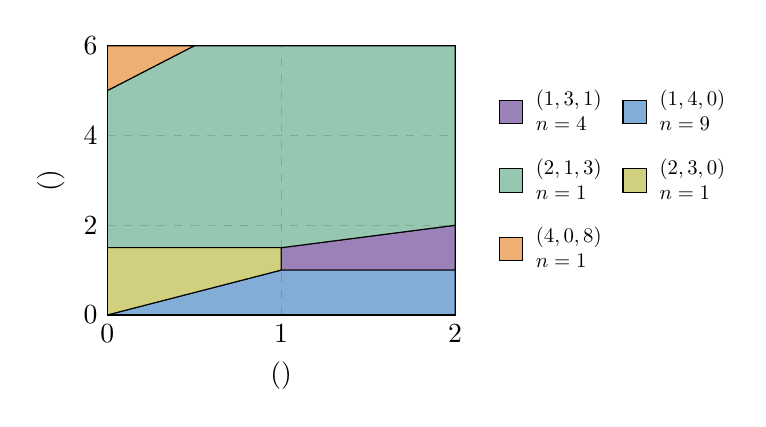
\begin{tikzpicture}
    \definecolor{c0}{HTML}{6F4C9B}
    \definecolor{c1}{HTML}{4D8AC6}
    \definecolor{c2}{HTML}{69B190}
    \definecolor{c3}{HTML}{BEBC48}
    \definecolor{c4}{HTML}{E78C35}
    \pgfplotsset{layers/mosaic/.define layer set={axis background,pre main,main,lines,marks,axis grid,axis ticks,axis lines,axis tick labels,axis descriptions,axis foreground}{/pgfplots/layers/standard}}
    \pgfplotsset{set layers=mosaic}
    \begin{axis}[
        width=6cm,
        height=5cm,
        clip mode=individual,
        legend style={
            anchor=west,
            at={(1.1, 0.5)},
            cells={anchor=west, align=left},
            nodes={scale=.75, transform shape},
            draw=none,
            column sep=3pt,
            /tikz/every even column/.append style={column sep=6pt},
            row sep=6pt,
        },
        legend columns=2,
        grid=both,
        grid style={black, opacity=.15, dashed},
        tick style={transparent},
        xtick distance=1,
        ytick distance=2,
        enlargelimits=false,
        xlabel={\(\cost(\evtD)\)},
        ylabel={\(\cost(\evtT)\)},
        area legend/.style={
            legend image code/.code={
                \draw [#1] (0cm,-0.15cm) rectangle (0.3cm,0.15cm);
            }, 
        },
    ]
    \addplot[area legend, black, fill=c0!70!white, mark=none] coordinates { (1.0, 1.0) (1.0, 1.5) (2.0, 2.0) (2.0, 1.0) (1.0, 1.0) };
    \addlegendentry{\((1, 3, 1)\)\\\(n=4\)}
    \addplot[area legend, black, fill=c1!70!white, mark=none] coordinates { (0.0, 0.0) (1.0, 1.0) (2.0, 1.0) (2.0, 0.0) (0.0, 0.0) };
    \addlegendentry{\((1, 4, 0)\)\\\(n=9\)}
    \addplot[area legend, black, fill=c2!70!white, mark=none] coordinates { (0.0, 1.5) (0.0, 5.0) (0.5, 6.0) (2.0, 6.0) (2.0, 2.0) (1.0, 1.5) (0.0, 1.5) };
    \addlegendentry{\((2, 1, 3)\)\\\(n=1\)}
    \addplot[area legend, black, fill=c3!70!white, mark=none] coordinates { (0.0, 0.0) (0.0, 1.5) (1.0, 1.5) (1.0, 1.0) (0.0, 0.0) };
    \addlegendentry{\((2, 3, 0)\)\\\(n=1\)}
    \addplot[area legend, black, fill=c4!70!white, mark=none] coordinates { (0.0, 5.0) (0.0, 6.0) (0.5, 6.0) (0.0, 5.0) };
    \addlegendentry{\((4, 0, 8)\)\\\(n=1\)}
    \end{axis}
\end{tikzpicture}

    \caption[Mosaïque des régions de coûts pour une instance de \(\recmodelDTLx\)-parcimonie]{
        Mosaïque des régions d’optimalité des coûts selon trois dimensions: nombre d’événements de duplication, de transfert et de perte.
        Les scénarios parcimonieux contenant des événements \(\evtTX\) sont écartés de ce diagramme.
        Celui-ci montre la tranche de l’espace des coûts pour \(\cost(\evtL) = 1\).
        La région \(\tup{2, 1, 3}\) contient la solution de la \cref{fig:adp-rec:rec-input}.
        \label{fig:adp-rec:rec-pareto}
    }
\end{figure}

Finalement, il est possible d’échantillonner des solutions quasioptimales en construisant une algèbre de Boltzmann comme décrit à la \cref{ex:adp:space-enum-sample:boltz}.
De cet ensemble peuvent être calculées efficacement les probabilités que chaque embranchement de \(T\) soit assigné à un événement donné ou à un hôte donné dans une solution moyenne (voir \cref{fig:adp-rec:rec-supports}) au travers du calcul des contributions externes introduit à la \cref{sec:adp:space-enum-sample:outside}, généralisant ainsi l’approche développée par~\textcite{Nguyen2013SupportMeasuresEstimate}.

\section{Parcimonie de groupes}\label{sec:adp-rec:set}

Le problème de la parcimonie de groupes, sous-jacent à la réconciliation segmentale, concerne l’inférence du contenu ancestral de synténies dans un arbre dont le contenu aux feuilles est connu.
Cette inférence s’appuie sur un modèle de gains et de pertes groupés, de sorte que chaque arête de l’arbre peut être étiquetée par un événement de gain qui fait apparaître simultanément une ou plusieurs nouvelles unités ou par une perte qui en fait disparaître.
Nous prendrons l’hypothèse de~Dollo, selon laquelle chaque unité est gagnée exactement une fois.

L’objectif du problème est de trouver un étiquetage de contenus ancestraux le plus parcimonieux en termes de gains et de pertes, en fonction du nombre d’événements et de leurs tailles respectives.
Plus précisément, chaque embranchement doit être étiqueté par un groupe de sorte à minimiser le coût formé par la somme, sur chaque branche \((v, v\child)\), de \(\cost_\evtG(|\syntenyOfExt(v\child) - \syntenyOfExt(v)|)\) et \(\cost_\evtL(|\syntenyOfExt(v) - \syntenyOfExt(v\child)|)\).
Un exemple d’instance pour le problème est présenté à la \cref{fig:adp-rec:set-example}.

\begin{problem}{Parcimonie de groupes}
    \probinput{Phylogénie \(T\);
               ensemble d’unités \(\geneFamilySet\);
               étiquetage \(\syntenyOf : \tleavs(T) \onto 2^{\geneFamilySet}\);\newline
               coûts \(\cost_\evtG, \cost_\evtL : \nat \onto \realpos\).}
    \proboutput{Affectation \(\syntenyOfExt : \tnodes(T) \onto 2^{\geneFamilySet}\) étendant \(\syntenyOf\) de coût minimum.}
\end{problem}

\begin{figure}[h]
    \capstart
    \centering
    %! TeX root = ../../main.tex
% vim: set spelllang=fr:
\begin{tikzpicture}[xscale=-1]
    \begin{scope}
        \graph[
            phylogenetic tree layout,
            evolutionary unit length=0.7cm,
            nodes={font=\small\strut, inner sep=0pt},
            length=1,
        ]{
            tf / [coordinate] -- {
                tc / [coordinate] -- {
                    tb / [coordinate] -- {
                        ta / [coordinate] -- {
                            t1 / b,
                            t2 / bc,
                        },
                        t3 / bce [>length=2],
                    },
                    t4 / ac [>length=3],
                },
                te / [coordinate] -- {
                    t5 / abd [>length=3],
                    td / [coordinate] -- {
                        t6 / bdf [>length=2],
                        t7 / bdfg [>length=2],
                    },
                },
            }
        };
    \end{scope}
    \draw[separator rule] (-3.2, -3) -- ++(0, 3);
    \begin{scope}[shift={(-7.5, 0)}]
        \graph[
            phylogenetic tree layout,
            evolutionary unit length=0.7cm,
            nodes={font=\small\strut, inner ysep=0pt},
            length=1,
        ]{
            tf / abcdef -- {
                tc / abcdef -- {
                    tb / bce [>edge node={node [loss={black}{adf}{left}] {}}] -- {
                        ta / bce -- {
                            t1 / b [>edge node={node [loss={black}{ce}{left}] {}}],
                            t2 / bc [>edge node={node [loss={black}{e}{right}] {}}],
                        },
                        t3 / bce [>length=2],
                    },
                    t4 / ac [>length=3, >edge node={node [loss={black}{bdef}{right}] {}}],
                },
                te / abcdef -- {
                    t5 / abd [>length=3, >edge node={node [loss={black}{cef}{right}] {}}],
                    td / bdf [>edge node={node [loss={black}{ace}{right}] {}}] -- {
                        t6 / bdf [>length=2],
                        t7 / bdfg [>length=2, >edge node={node [gain={black}{g}{right}] {}}],
                    },
                },
            }
        };
        \draw (tf) edge node[gain={black}{abcdef}{right}] {} ($(tf)+(0,.66)$);
    \end{scope}
\end{tikzpicture}

    \caption[Instance et solution à un problème de parcimonie de groupes]{
        \emph{(Gauche.)} Exemple d’entrée pour le problème de parcimonie de groupes.
        Chaque feuille est étiquetée par un ensemble d’unités chacune représentée par une lettre différente.
        L’ordre dans lequel celles-ci sont inscrites est sans importance.
        Cet exemple est tiré de \textcite{Gascon2026GeneRepertoireEvolution}.
        \emph{(Droite.)} Une solution possible pour l’entrée donnée.
        Les événements de gain sont représentés par des demi-cercles ouverts vers le bas et ceux de perte par des demi-cercles ouverts vers le haut, à côté desquels le groupe d’unités gagnées ou perdues est indiqué.
        \label{fig:adp-rec:set-example}
    }
\end{figure}

Une première version du problème a été étudiée par \textcite{Delabre2020EvolutionSegmentalDuplications} en ignorant la taille des pertes et en supposant que toutes les unités soient gagnées dès la racine de l’arbre.
Au cours du printemps~2025, Corélie~\textsc{Godefroid} a étudié la version de ce problème étendue pour également placer les événements de gains de manière optimale.
Ces idées ont été développées par Mathieu~\textsc{Gascon}, menant à un article présenté à la conférence RECOMB-CG~2026 \parencite{Gascon2026GeneRepertoireEvolution}.
La solution présentée dans la suite de cette section est basée sur ce travail.

\subsection{Réduction du problème}

Observons que ce problème peut être vu comme portant sur la taille des groupes ancestraux et non sur leur contenu.
En effet, puisque les fonctions de coûts considérées dépendent uniquement du nombre d’événements de gain et de perte et du nombre d’unités gagnées et perdues, deux solutions qui infèrent les mêmes tailles de groupes ancestraux sont indistinguables du point de vue de leur coût et seront considérées comme équivalentes dans la suite.
Le problème se rapproche ainsi de celui résolu par le programme Count de \textcite{Csuros2010CountEvolutionaryAnalysis} qui infère des profils de nombre de copies ancestrales d’une famille de gènes sur la base d’un modèle probabiliste.

Certaines contraintes existent toutefois sur les tailles des groupes ancestraux.
À chaque embranchement \(v \in \tnodes(T)\), l’ensemble des unités~\(\geneFamilySet\) peut être partitionné en trois sous-ensembles \(\geneFamilySet = \xmin(v) \cup \xin(v) \cup \xout(v)\), où:
\begin{compactitemize}
    \item \(\xmin(v)\) est l’ensemble des unités dont le \emph{lca} est un ancêtre de \(v\) et qui apparaissent dans au moins une feuille du sous-arbre de \(v\);
    \item \(\xout(v)\) est l’ensemble des unités qui n’apparaissent dans aucune feuille du sous-arbre de \(v\);
    \item \(\xin(v)\) est l’ensemble des unités dont le \emph{lca} est un descendant strict de \(v\).
\end{compactitemize}
En raison de l’hypothèse de Dollo, les unités de \(\xmin(v)\) apparaissent dans l’ensemble \(\syntenyOfExt(v)\) dans toute solution.
À l’inverse, \(\xout(v)\) et \(\xin(v)\) contiennent des unités qui peuvent y apparaître de manière optionnelle: dans le cas de \(\xout(v)\), celles-ci peuvent être librement perdues dans la branche menant à \(v\) et, dans le cas de \(\xin(v)\), elles peuvent y être librement gagnées.

Pour représenter l’espace des solutions du problème, nous fixons donc pour signature l’ensemble d’opérateurs \(\algsignset = \{\algnull,\allowbreak \algplus,\allowbreak \evLeaf,\allowbreak \evGain,\allowbreak \evLoss,\allowbreak \evSplit\}\) définis comme suit:
\begin{itemize}
    \item \(\evLeaf\) représente une feuille de l’arbre;
    \item \(\evGain_N(h)\) et \(\evLoss_N(h)\) représentent respectivement un gain ou une perte de \(N\) unités;
    \item \(\evSplit_{G_L,G_R,L}(h_L, h_R)\) représente un embranchement de l’arbre au niveau duquel \(G_L+G_R\) unités restent à gagner, dont \(G_L\) dans le sous-arbre à gauche et \(G_R\) dans le sous-arbre à droite, et \(L\) unités restent à perdre.
\end{itemize}

\subsection{Algèbres d’évaluation}

Cette signature permet, pour deux fonctions de coûts \(\cost_\evtG\) et \(\cost_\evtL\) données, de définir l’algèbre d’optimisation additive \(\alminplus_{\cost_\evtG,\cost_\evtL}\) suivante\\
\threecols{.33\textwidth}{.33\textwidth}{.33\textwidth}{
\begin{align*}
    \algnull &= \infty \\
    \evGain_N(h) &= h + \cost_\evtG(N)
\end{align*}
}{
\begin{align*}
    \algplus &= \min \\
    \evLoss_N(h) &= h + \cost_\evtL(N)
\end{align*}
}
{
\begin{align*}
    \evLeaf &= 0 \\
    \evSplit_{G,G',L}(h_L, h_R) &= h_L + h_R.
\end{align*}
}

Comme précédemment, cette algèbre peut être adaptée en algèbre de Boltzmann ou de Pareto.

Notons que les fonctions \(\cost_\evtG\) et \(\cost_\evtL\) peuvent être arbitraires.
Un coût constant, c’est-à-dire de la forme \(\cost_e(n) = b_e\) si \(n \ge 1\) et \(0\) sinon, pour une constante \(b_e \in \realpos \cup \{\infty\}\), permet de minimiser le nombre d’événements sans prendre en compte la taille des gains et des pertes.
Le problème devient alors équivalent au problème sous-jacent à la réconciliation segmentale de \textcite{Delabre2020EvolutionSegmentalDuplications} et des \cref{chap:superdtl,chap:synesth}.
Les solutions obtenues avec ces coûts ont tendance à regrouper beaucoup d’événements et à engendrer une quantité excessive de pertes.

Un coût linéaire, c’est-à-dire de la forme \(\cost_e(n) = a_en\) pour une constante \(a_e \in \realpos \cup \{\infty\}\), permet de rechercher les solutions minimisant la taille totale des événements.
Il rend cependant le problème équivalent à la parcimonie de Dollo individuelle, puisque les unités peuvent alors être considérées comme évoluant indépendamment.

Plus généralement, un coût affine de la forme \(\cost_e(n) = a_en + b_e\) si \(n \ge 1\) et \(0\) sinon, pour deux constantes \(a_e, b_e \in \realpos \cup \{\infty\}\), prend simultanément en compte la dépendance entre les unités étudiées tout en accordant une préférence aux solutions plus parcimonieuses minimisant globalement la taille des événements.
Dans la suite, les constantes \(b_e\) sont appelées les coûts d’ouverture et les constantes \(a_e\) les coûts d’extension des gains ou des pertes.

\subsection{Grammaire de structure}

L’espace des solutions peut être décrit par une grammaire \(\gramset\) de dimension trois.
La première dimension \(T\) représente le sous-arbre traité.
La seconde dimension \(G\) représente le nombre d’unités restant à gagner dans le sous-arbre traité.
La troisième dimension \(L\) représente le nombre d’unités de l’ensemble \(\xout\) présentes, c’est-à-dire qui ont déjà été gagnées mais qui n’apparaissent dans aucune feuille du sous-arbre traité.
La grammaire utilise trois prédicats définis ainsi:
\begin{compactitemize}
    \item \(\gSplit[T, G, L]\) représente les solutions dont la racine est \(T\) et en dessous de laquelle il reste à gagner \(G\) unités et à en perdre \(L\);
    \item \(\gBranch[T, G, L]\) et \(\gBranch'[T, G, L]\) représentent les solutions qui ajoutent des événements unaires de perte et de gain au-dessus de \(T\).
\end{compactitemize}
À chaque niveau de la solution, il faut s’assurer que \(G\) ne dépasse pas le nombre d’unités qui peuvent être potentiellement gagnées dans le sous-arbre traité.
Plus précisément, pour chaque embranchement \(v\), notons \(\xlca(v)\) l’ensemble qui rassemble toutes les unités dont le \(\lca\) est un descendant de \(v\), c’est-à-dire les unités qui peuvent être gagnées en \(v\) ou en dessous.
Chaque appel à l’un des trois prédicats n’amène ainsi à une solution valide que si \(G \le |\xlca(v)|\).

L’ensemble des solutions est constitué des termes dérivés de \(\gBranch[T, |\geneFamilySet|, 0]\), où \(T\) est l’arbre d’entrée et \(\geneFamilySet\) l’ensemble de toutes les unités.
Les clauses de la grammaire sont:
{\allowdisplaybreaks
\begin{subequations}
\begin{align}
    \gSplit[(), 0, 0] &\rightarrow \evLeaf \label{eq:adp-rec:set-split-leaf} \\[2ex]
    \begin{aligned}
        &\gSplit[t(t\lchild(T_L)\,t\rchild(T_R)), G_L + G_R, L] \\
        \rightarrow\ & \evSplit_{G_L, G_R, L}(
            \begin{aligned}[t]
                &\gBranch[t\lchild(T_L), G_L, L + |\xlca(t\rchild)| - G_R + |\xmin(t) - \xmin(t\lchild)|], \\
                &\gBranch[t\rchild(T_R), G_R, L + |\xlca(t\lchild)| - G_L + |\xmin(t) - \xmin(t\rchild)|])
            \end{aligned} \\
        &\text{\itshape\small (seulement lorsque \(|\xlca(t\lchild)| \ge G_L\) and \(|\xlca(t\rchild)| \ge G_R\))}
    \end{aligned} \span \label{eq:adp-rec:set-split-inner}\\[2ex]
    \gBranch[T, G, L_H + L_D] &\rightarrow \evLoss_{L_H}(\gBranch'[T, G, L_D]) \label{eq:adp-rec:set-split-loss}\\
    \gBranch'[T, G_H + G_D, L] &\rightarrow \evGain_{G_H}(\gSplit[T, G_D, L]). \label{eq:adp-rec:set-split-gain}
\end{align}
\end{subequations}}%
La clause \labelcref{eq:adp-rec:set-split-inner} s’applique à chaque embranchement de \(T\).
Chacune des \(G\) unités qui restent à gagner à un certain embranchement peuvent être gagnés soit dans le sous-arbre gauche, soit dans le sous-arbre droit, d’où la décomposition en \(G = G_L + G_R\).
Chacune des \(L\) unités qui sont issues de l’ensemble \(\xout(t)\) sont par définition éléments des ensembles \(\xout(t\lchild)\) et \(\xout(t\rchild)\), auxquels il faut ajouter les unités qui seront gagnées de l’autre côté (resp. \(|\xmin(t) - \xmin(t\lchild)|\) et \(|\xmin(t) - \xmin(t\rchild)|\)) et celles qui ont déjà été gagnées mais ne sont plus nécessaires dans le sous-arbre actuel (resp. \(|\xlca(t\rchild)| - G_R\) et \(|\xlca(t\lchild)| - G_L\)).

Les clauses \labelcref{eq:adp-rec:set-split-loss,eq:adp-rec:set-split-gain} introduisent respectivement une perte et un gain d’un nombre d’unités au plus égal à la valeur courante de \(L\) ou de \(G\).

Nous conjecturons que cette grammaire est non ambigüe et qu’elle est canonique pour le problème de parcimonie de groupes, c’est-à-dire que chaque scénario est énuméré exactement une fois, en considérant uniquement la taille des groupes et non leur contenu exact.

Grâce à l’\cref{alg:seq-yield-parser}, cette grammaire correspond automatiquement à un algorithme de programmation dynamique.
En vertu du \cref{thm:adp:gram-hedge-complex}, sa complexité en temps est \(\bigo(nf^3)\), où \(n\) est la taille de \(T\) et \(f\) le nombre d’unités dans \(\geneFamilySet\).
Le fait de séparer les deux clauses \labelcref{eq:adp-rec:set-split-loss,eq:adp-rec:set-split-gain} est nécessaire pour conserver une complexité en \(f^3\) au lieu de \(f^4\).

Les solutions de l’espace de solutions ainsi engendré ne décrivent pas directement le contenu des groupes ancestraux, mais seulement leurs tailles respectives.
Cependant, il est aisé de déterminer un exemple de contenu pour toute solution en utilisant les ensembles \(\xmin(v)\), \(\xin(v)\) et \(\xout(v)\).

\subsection{Résultats}

L’application de la grammaire \(\gramset\) sur l’entrée à gauche de la \cref{fig:adp-rec:set-example} engendre un certain espace de solutions sur lequel différentes algèbres peuvent être appliquées.
En utilisant l’algèbre~\(\alminplus_{\cost_\evtG,\cost_\evtL}\) avec un coût constant, nous obtenons un nombre d’événements minimal de~8.
En combinant cette algèbre avec l’algèbre de traçage \(\altrace(\algsignset)\) grâce au combinateur lexicographique, il est possible de construire la solution atteignant ce coût présentée à droite de la \cref{fig:adp-rec:set-example}.

L’utilisation d’un coût affine fixant le coût d’ouverture des gains et des pertes à \(b_\evtL = b_\evtG = 3\) et leur coût d’extension à \(a_\evtL = a_\evtG = 1\) permet d’identifier la solution présentée à gauche de la \cref{fig:adp-rec:set-solutions}.
Avec l’algèbre de Pareto, nous pouvons construire le diagramme de la \cref{fig:adp-rec:set-pareto} qui montre qu’il existe plusieurs classes de solutions parcimonieuses obtenues en faisant varier les différents paramètres de coûts.

Finalement, il est possible d’échantillonner des solutions quasioptimales en construisant une algèbre de Boltzmann comme décrit à la \cref{ex:adp:space-enum-sample:boltz}.
Cet ensemble peut être caractérisé en calculant l’espérance de la taille des groupes ancestraux au travers du calcul des contributions externes introduit à la \cref{sec:adp:space-enum-sample:outside}, comme présenté à droite de la \cref{fig:adp-rec:set-solutions}.

\begin{figure}[p]
    \capstart
    \centering
    \begin{tikzpicture}[xscale=-1]
    \begin{scope}
        \graph[
            phylogenetic tree layout,
            evolutionary unit length=0.95cm,
            nodes={font=\small\strut, inner ysep=0pt},%, draw, rounded corners},
            length=1,
        ]{
            tf / abd -- {
                tc / abcd [>edge node={node [gain={black}{c}{left}] {}}] -- {
                    tb / bc [>edge node={node [loss={black}{ad}{left}] {}}] -- {
                        ta / bc -- {
                            t1 / b [>edge node={node [loss={black}{c}{left}] {}}],
                            t2 / bc,
                        },
                        t3 / bce [>length=2, >edge node={node [gain={black}{e}{right}] {}}],
                    },
                    t4 / ac [>length=3, >edge node={node [loss={black}{bd}{right}] {}}],
                },
                te / abd -- {
                    t5 / abd [>length=3],
                    td / bdf [
                        >edge node={node [pos=.25, loss={black}{a}{right}] {}},
                        >edge node={node [pos=.7, gain={black}{f}{right}] {}},
                    ] -- {
                        t6 / bdf [>length=2],
                        t7 / bdfg [>length=2, >edge node={node [gain={black}{g}{right}] {}}],
                    },
                },
            }
        };
        \draw (tf) edge node[gain={black}{abd}{right}] {} ($(tf)+(0,.66)$);
    \end{scope}

    \draw[separator rule] (-3.6, -4.2) -- ++(0, 4.8);
    \begin{scope}[shift={(-8,0)}]
        % temp=1, gain=loss=3, ext=1
        % 1
        % loss=1.044
        % gain=0.000
        % size=1.000

        % 2
        % loss=0.044
        % gain=0.000
        % size=2.000

        % A
        % loss=0.160
        % gain=0.000
        % size=2.044

        % 3
        % loss=0.050
        % gain=0.846
        % size=3.000

        % B
        % loss=1.570
        % gain=0.025
        % size=2.204

        % 4
        % loss=1.748
        % gain=0.000
        % size=2.000

        % C
        % loss=0.117
        % gain=0.706
        % size=3.748

        % 5
        % loss=0.467
        % gain=0.000
        % size=3.000

        % 6
        % loss=0.369
        % gain=0.000
        % size=3.000

        % 7
        % loss=0.087
        % gain=0.718
        % size=4.000

        % D
        % loss=1.123
        % gain=1.025
        % size=3.369

        % E
        % loss=0.213
        % gain=0.521
        % size=3.467

        % F
        % loss=0.000
        % gain=3.159
        % size=3.159
        \graph[
            phylogenetic tree layout,
            evolutionary unit length=0.95cm,
            nodes={font=\small\strut, inner ysep=0pt},
            length=1,
        ]{
            tf / 3.159 -- {
                tc / 3.748 [
                    >edge node={node [pos=.25, loss={black}{0.117}{left}] {}},
                    >edge node={node [pos=.7, gain={black}{0.706}{left}] {}},
                ] -- {
                    tb / 2.204 [
                        >edge node={node [pos=.25, loss={black}{1.570}{left}] {}},
                        >edge node={node [pos=.7, gain={black}{0.025}{left}] {}},
                    ] -- {
                        ta / 2.044 [
                            >edge node={node [pos=.25, loss={black}{0.160}{left}] {}},
                            >edge node={node [pos=.7, gain={black}{0.000}{left}] {}},
                        ] -- {
                            t1 / b [
                                >edge node={node [pos=.25, loss={black}{1.044}{left}] {}},
                                >edge node={node [pos=.6, gain={black}{0.000}{left}] {}},
                            ],
                            t2 / bc [
                                >edge node={node [pos=.25, loss={black}{0.044}{right}] {}},
                                >edge node={node [pos=.6, gain={black}{0.000}{right}] {}},
                            ],
                        },
                        t3 / bce [
                            >length=2,
                            >edge node={node [pos=.25, loss={black}{0.050}{right}] {}},
                            >edge node={node [pos=.4, gain={black}{0.846}{right}] {}},
                        ],
                    },
                    t4 / ac [
                        >length=3,
                        >edge node={node [pos=.2, loss={black}{1.748}{right}] {}},
                        >edge node={node [pos=.32, gain={black}{0.000}{right}] {}},
                    ],
                },
                te / 3.467 [
                    >edge node={node [pos=.25, loss={black}{0.213}{right}] {}},
                    >edge node={node [pos=.7, gain={black}{0.521}{right}] {}},
                ] -- {
                    t5 / abd [
                        >length=3,
                        >edge node={node [pos=.2, loss={black}{0.467}{left}] {}},
                        >edge node={node [pos=.32, gain={black}{0.000}{left}] {}},
                    ],
                    td / 3.369 [
                        >edge node={node [pos=.25, loss={black}{1.123}{right}] {}},
                        >edge node={node [pos=.7, gain={black}{1.025}{right}] {}},
                    ] -- {
                        t6 / bdf [
                            >length=2,
                            >edge node={node [pos=.45, loss={black}{0.369}{left}] {}},
                            >edge node={node [pos=.6, gain={black}{0.000}{left}] {}},
                        ],
                        t7 / bdfg [
                            >length=2,
                            >edge node={node [pos=.45, loss={black}{0.087}{right}] {}},
                            >edge node={node [pos=.6, gain={black}{0.718}{right}] {}},
                        ],
                    },
                },
            }
        };
        \draw (tf) edge
            node[pos=.25, gain={black}{\(3.159\)}{right}] {}
            node[pos=.7, loss={black}{\(0.000\)}{right}] {}
        ($(tf)+(0,.66)$);
    \end{scope}
\end{tikzpicture}

    \caption[Solution alternative et espérance des tailles des groupes]{
        \emph{(Gauche.)}
        Solution optimale avec 9~événements pour un coût d’ouverture de~3 et d’extension de~1.
        \emph{(Droite.)}
        Espérances de la taille des pertes, des gains et des contenus dans un scénario moyen de la distribution de Boltzmann avec température \(T=1\) et coût d’ouverture de \(3\) et d’extension de \(1\).
    }
    \label{fig:adp-rec:set-solutions}
\end{figure}

\begin{figure}[p]
    \capstart
    \centering
    \begin{tikzpicture}
    \definecolor{c0}{HTML}{6F4C9B}
    \definecolor{c1}{HTML}{5568B8}
    \definecolor{c2}{HTML}{4D8AC6}
    \definecolor{c3}{HTML}{59A5A9}
    \definecolor{c4}{HTML}{69B190}
    \definecolor{c5}{HTML}{8CBC68}
    \definecolor{c6}{HTML}{BEBC48}
    \definecolor{c7}{HTML}{DDAA3C}
    \definecolor{c8}{HTML}{E78C35}
    \definecolor{c9}{HTML}{DA2222}
    \pgfplotsset{layers/mosaic/.define layer set={axis background,pre main,main,lines,marks,axis grid,axis ticks,axis lines,axis tick labels,axis descriptions,axis foreground}{/pgfplots/layers/standard}}
    \pgfplotsset{set layers=mosaic}
    \begin{axis}[
        width=7.5cm,
        height=6.5cm,
        clip mode=individual,
        legend style={
            anchor=west,
            at={(1.1, 0.5)},
            cells={anchor=west, align=left},
            nodes={scale=.75, transform shape},
            draw=none,
            column sep=4pt,
            /tikz/every column/.append style={column sep=4pt},
        },
        legend columns=3,
        grid=both,
        grid style={black, opacity=.15, dashed},
        tick style={transparent},
        xtick distance=1,
        ytick distance=2,
        enlargelimits=false,
        xlabel={\(b_{\kern1pt\evtL}\)},
        ylabel={\(b_\evtG\)},
        area legend/.style={
            legend image code/.code={
                \draw [#1] (0cm,-0.15cm) rectangle (0.3cm,0.15cm);
            }, 
        },
        short line legend/.style={
            legend image code/.code={
                \draw [mark repeat=2,mark phase=2,##1]
                    plot coordinates {
                        (0cm,0cm)
                        (0.15cm,0cm)
                        (0.3cm,0cm)
                    };
            },
        }, 
    ]
    \addplot[area legend, black, fill=c0!70!white, mark=none] coordinates { (1.0, 2.0) (3.0, 4.0) (5.0, 5.0) (5.0, 2.0) (1.0, 2.0) };
    \addlegendentry{\((4, 5, 6)\)\\\(n=1\)}
    \addplot[area legend, black, fill=c1!70!white, mark=none] coordinates { (0.0, 0.0) (0.0, 1.0) (1.0, 2.0) (5.0, 2.0) (5.0, 0.0) (0.0, 0.0) };
    \addlegendentry{\((4, 6, 4)\)\\\(n=1\)}
    \addplot[area legend, black, fill=c2!70!white, mark=none] coordinates { (3.0, 4.0) (3.0, 6.0) (4.0, 8.0) (5.0, 9.0) (5.0, 5.0) (3.0, 4.0) };
    \addlegendentry{\((5, 3, 11)\)\\\(n=1\)}
    \addplot[short line legend, black, line width=2pt, line cap=round, postaction={draw, c0!70!white, line width=1.3pt}, on layer=lines] coordinates { (1.0, 2.0) (3.0, 4.0) };
    \addlegendentry{\((5, 4, 7)\)\\\(n=3\)}
    \addplot[short line legend, black, line width=2pt, line cap=round, postaction={draw, c1!70!white, line width=1.3pt}, on layer=lines] coordinates { (4.0, 8.0) (5.0, 9.0) };
    \addlegendentry{\((6, 2, 15)\)\\\(n=2\)}
    \addplot[area legend, black, fill=c3!70!white, mark=none] coordinates { (1.0, 2.0) (1.0, 4.0) (3.0, 6.0) (3.0, 4.0) (1.0, 2.0) };
    \addlegendentry{\((6, 3, 8)\)\\\(n=1\)}
    \addplot[short line legend, black, line width=2pt, line cap=round, postaction={draw, c2!70!white, line width=1.3pt}, on layer=lines] coordinates { (0.0, 1.0) (1.0, 2.0) };
    \addlegendentry{\((6, 4, 6)\) et\\\((5, 5, 5)\)\\\(n=4\)}
    \addplot[area legend, black, fill=c4!70!white, mark=none] coordinates { (3.0, 8.0) (3.0, 9.0) (5.0, 9.0) (4.0, 8.0) (3.0, 8.0) };
    \addlegendentry{\((7, 1, 19)\)\\\(n=1\)}
    \addplot[area legend, black, fill=c5!70!white, mark=none] coordinates { (1.0, 4.0) (1.0, 5.00000000000001) (2.0, 7.0) (3.0, 8.0) (4.0, 8.0) (3.0, 6.0) (1.0, 4.0) };
    \addlegendentry{\((7, 2, 11)\)\\\(n=1\)}
    \addplot[area legend, black, fill=c6!70!white, mark=none] coordinates { (0.0, 1.0) (0.0, 3.0) (1.0, 4.0) (1.0, 2.0) (0.0, 1.0) };
    \addlegendentry{\((7, 3, 7)\)\\\(n=1\)}
    \addplot[area legend, black, fill=c7!70!white, mark=none] coordinates { (2.0, 7.0) (2.0, 9.0) (3.0, 9.0) (3.0, 8.0) (2.0, 7.0) };
    \addlegendentry{\((8, 1, 16)\)\\\(n=1\)}
    \addplot[area legend, black, fill=c8!70!white, mark=none] coordinates { (0.0, 3.0) (0.0, 4.0) (1.0, 5.0) (1.0, 4.0) (0.0, 3.0) };
    \addlegendentry{\((8, 2, 10)\)\\\(n=1\)}
    \addplot[area legend, black, fill=c9!70!white, mark=none] coordinates { (0.0, 4.0) (0.0, 9.0) (2.0, 9.0) (2.0, 7.0) (1.0, 5.0) (0.0, 4.0) };
    \addlegendentry{\((9, 1, 14)\)\\\(n=1\)}
    \end{axis}
\end{tikzpicture}

    \caption[Mosaïque des régions de coûts pour une instance de parcimonie de groupes]{
        Mosaïque des régions d’optimalité des coûts selon trois dimensions: nombre d’événements de perte, nombre d’événements de gain, et taille totale des pertes.
        La taille totale des gains n’est pas comptabilisée afin de se réduire à trois dimensions au lieu de quatre.
        Ceci correspond à des coûts affines de la forme \(\cost_\evtG(n) = b_\evtG\) et \(\cost_\evtL(n) = a_\evtL n + b_\evtL\).
        Le diagramme montre la tranche de l’espace des coûts pour \(a_\evtL = 1\).
        La région \(\tup{5, 3, 11}\) inclut le coût unitaire et l’unique solution optimale pour ce coût est celle illustrée dans la \cref{fig:adp-rec:set-example}.
        La solution à gauche de la \cref{fig:adp-rec:set-solutions} est l’unique optimale dans la région \(\tup{4, 5, 6}\).
        Les régions \(\tup{7, 1, 19}\), \(\tup{8, 1, 16}\) et \(\tup{9, 1, 14}\) contiennent les trois solutions qui placent tous les gains à la racine avec \(7\), \(8\) ou \(9\) événements de perte.
    }
    \label{fig:adp-rec:set-pareto}
\end{figure}

\section{Réconciliation segmentale}\label{sec:adp-rec:both}

Le problème de réconciliation segmentale, introduit à la \cref{sec:reconciliation:multiple:segmental}, peut être vu comme demandant de résoudre simultanément un problème de réconciliation bilatérale et un problème de parcimonie d’ensembles, tout en respectant certaines contraintes supplémentaires.

Nous proposons, pour résoudre ce problème, de combiner les grammaires \(\gramrec\) et \(\gramset\) en une grammaire \(\gramseq\).
Cette approche offre une voie simplifiée pour retrouver les constructions des \cref{chap:superdtl,chap:synesth}.
Au meilleur de nos connaissances, aucune méthode générale n’est actuellement connue pour combiner de telles grammaires.
Dans la suite, nous réalisons donc une construction ad hoc dont des principes plus généraux pourront être tirés dans des recherches ultérieures.

Intuitivement, cette combinaison est réalisée en prenant le produit cartésien des ensembles de prédicats des deux grammaires, puis de leurs ensembles de clauses.
Chaque paire de prédicats ainsi obtenue agit simultanément sur les dimensions \(T\), \(S\) et \(N\) de \(\gramrec\) et sur les dimensions \(T\), \(G\) et \(L\) de \(\gramset\), la dimension \(T\) étant partagée entre les deux grammaires.
Chaque paire de clauses est combinée lorsque les motifs de leurs têtes sont compatibles sur cette dimension partagée.
Les corps des clauses sont combinés de manière ad hoc.
Les clauses résultantes sont présentées ci-dessous et dans le \cref{tab:adp-rec:product}.
{\allowdisplaybreaks
\begin{subequations}
\begin{align}
    \gRecSplit[t(), v(), 0, 0] &\rightarrow \evLeaf_{t,v}
    \qquad\text{\itshape\small (seulement lorsque \(\llmap(t) = v\))} \label{eq:adp-rec:comb-grammar-leaf}\\[2ex]
    \begin{aligned}
        &\gRecSplit[t(t'(T') \mid t''(T'')), v((S_L)(S_R)), G_L + G_R, L] \\
        \rightarrow\ & \evSpe_{t,v,G_L,G_R,L}(
            \begin{aligned}[t]
                &\gRecPathBranch[t'(T'), (S_L), 0, G_L, L + |\xlca(t'')| - G_R + |\xmin(t) - \xmin(t')|], \\
                &\gRecPathBranch[t''(T''), (S_R), 0, G_R, L + |\xlca(t')| - G_L + |\xmin(t) - \xmin(t'')|])
            \end{aligned} \\[-2ex]
        \intertext{\hspace*{3em}\itshape\small (seulement lorsque \(|\xlca(t')| \ge G_L\) and \(|\xlca(t'')| \ge G_R\))}
    \end{aligned} \span \label{eq:adp-rec:comb-grammar-spe} \\[1ex]
    \begin{aligned}
        &\gRecSplit[t(t'(T') \mid t''(T'')), v(S), G_L + G_R, L] \\
        \rightarrow\ & \evDup_{t,v,G_L,G_R,L}(
            \begin{aligned}[t]
                &\gRecPathBranch[t'(T'), v(S), 0, G_L, 0], \\
                &\gRecPathBranch[t''(T''), v(S), 0, G_R, L + |\xlca(t')| - G_L + |\xmin(t) - \xmin(t'')|])
            \end{aligned} \\[-2ex]
        \intertext{\hspace*{3em}\itshape\small (seulement lorsque \(|\xlca(t')| \ge G_L\) and \(|\xlca(t'')| \ge G_R\))}
    \end{aligned} \span \label{eq:adp-rec:comb-grammar-dup} \\[1ex]
    \begin{aligned}
        &\gRecSplit[t(t'(T') \mid t''(T'')), v(S), G_L + G_R, L] \\
        \rightarrow\ & \evTr_{t,v,G_L,G_R,L}(
            \begin{aligned}[t]
                &\gRecOutBranch[t'(T'), v(S), G_L, 0], \\
                &\gRecPathBranch[t''(T''), v(S), 0, G_R, L + |\xlca(t')| - G_L + |\xmin(t) - \xmin(t'')|])
            \end{aligned} \\[-2ex]
        \intertext{\hspace*{3em}\itshape\small (seulement lorsque \(|\xlca(t')| \ge G_L\) and \(|\xlca(t'')| \ge G_R\))}
    \end{aligned} \span \label{eq:adp-rec:comb-grammar-tr} \\[1ex]
    \gRecPathBranch[T, s((S') \mid S''), N, G, L]
        &\rightarrow \gRecPathBranch[T, S', N+1, G, L] \label{eq:adp-rec:comb-grammar-path-down} \\
    \gRecPathBranch[T, S, N, G, L_H + L_D]
        &\rightarrow \evSkip_N(\evLoss_{L_H}(\gRecBranchEnd[T, S, G, L_D])) \label{eq:adp-rec:comb-grammar-path-end} \\[2ex]
    \gRecInBranch[T, s((S') \mid S''), G, L] &\rightarrow \gRecInBranch[T, S', G, L] \label{eq:adp-rec:comb-grammar-in-down} \\
    \gRecInBranch[T, S, G, L_H + L_D] &\rightarrow \evLoss_{L_H}(\gRecBranchEnd[T, S, G, L_D]) \label{eq:adp-rec:comb-grammar-in-end} \\[2ex]
    \gRecOutBranch[T, S \text{ frère de } S', G, L] &\rightarrow \gRecInBranch[T, S', G, L] \label{eq:adp-rec:comb-grammar-out-side} \\
    \gRecOutBranch[T, P \text{ parent de } S, G, L] &\rightarrow \gRecOutBranch[T, P, G, L] \label{eq:adp-rec:comb-grammar-out-up} \\
    \gRecBranchEnd[T, S, G_H + G_D, L] &\rightarrow \evGain_{G_H}(\gRecSplit[T, S, G_D, L]) \label{eq:adp-rec:comb-grammar-gain}
\end{align}
\end{subequations}}

\begin{table}[h]
    \capstart
    \centering
    \begin{tabular}{cccccccccccc}
        \toprule
        & \textbf{\ref{eq:adp-rec:bilateral-grammar-leaf}}
        & \textbf{\ref{eq:adp-rec:bilateral-grammar-spe}}
        & \textbf{\ref{eq:adp-rec:bilateral-grammar-dup}}
        & \textbf{\ref{eq:adp-rec:bilateral-grammar-tr}}
        & \textbf{\ref{eq:adp-rec:bilateral-grammar-path-down}}
        & \textbf{\ref{eq:adp-rec:bilateral-grammar-path-end}}
        & \textbf{\ref{eq:adp-rec:bilateral-grammar-in-down}}
        & \textbf{\ref{eq:adp-rec:bilateral-grammar-in-end}}
        & \textbf{\ref{eq:adp-rec:bilateral-grammar-out-side}}
        & \textbf{\ref{eq:adp-rec:bilateral-grammar-out-up}}
        & \(\circlearrowright\)
        \\
        \midrule
        \textbf{\ref{eq:adp-rec:set-split-leaf}}
        & \ref{eq:adp-rec:comb-grammar-leaf}
        & ---
        & ---
        & ---
        & ---
        & ---
        & ---
        & ---
        & ---
        & ---
        & ---
        \\
        \midrule
        \textbf{\ref{eq:adp-rec:set-split-inner}}
        & ---
        & \ref{eq:adp-rec:comb-grammar-spe}
        & \ref{eq:adp-rec:comb-grammar-dup}\textsuperscript{*}
        & \ref{eq:adp-rec:comb-grammar-tr}\textsuperscript{*}
        & ---
        & ---
        & ---
        & ---
        & ---
        & ---
        & ---
        \\
        \midrule
        \textbf{\ref{eq:adp-rec:set-split-loss}}
        & ---
        & ---
        & ---
        & ---
        & \ref{eq:adp-rec:comb-grammar-path-down}
        & \ref{eq:adp-rec:comb-grammar-path-end}
        & \ref{eq:adp-rec:comb-grammar-in-down}
        & \ref{eq:adp-rec:comb-grammar-in-end}
        & ---
        & ---
        & ---
        \\
        \midrule
        \textbf{\ref{eq:adp-rec:set-split-gain}}
        & ---
        & ---
        & ---
        & ---
        & ---
        & ---
        & ---
        & ---
        & ---
        & ---
        & \ref{eq:adp-rec:comb-grammar-gain}
        \\
        \midrule
        \(\circlearrowright\)
        & ---
        & ---
        & ---
        & ---
        & ---
        & ---
        & ---
        & ---
        & \ref{eq:adp-rec:comb-grammar-out-side}
        & \ref{eq:adp-rec:comb-grammar-out-up}
        & ---
        \\
        \bottomrule
    \end{tabular}
    \caption[Paires de clauses des grammaires \(\gramrec\) et \(\gramset\) combinées pour former \(\gramseq\)]{
        Paires de clauses des grammaires \(\gramrec\) (\ref{eq:adp-rec:bilateral-grammar-leaf} à \ref{eq:adp-rec:bilateral-grammar-out-up}) et \(\gramset\) (\ref{eq:adp-rec:set-split-leaf} à \ref{eq:adp-rec:set-split-gain}) combinées pour former les clauses de la grammaire \(\gramseq\).
        Dans les clauses \labelcref{eq:adp-rec:comb-grammar-dup,eq:adp-rec:comb-grammar-tr} marquées d’un astérisque, l’un des deux arguments \(L\) a été remplacé par un~0.
        La dernière colonne correspond à une boucle \(\gRec[T, S] \rightarrow \gRec[T, S]\) et la dernière rangée à une boucle \(\gBranch[T, G, L] \rightarrow \gBranch[T, G, L]\) qui, bien qu’absentes des grammaires originales, sont nécessaires pour faire apparaître les clauses \labelcref{eq:adp-rec:comb-grammar-out-side}, \labelcref{eq:adp-rec:comb-grammar-out-up} et \labelcref{eq:adp-rec:comb-grammar-gain}.
        \label{tab:adp-rec:product}
    }
\end{table}

Dans le modèle de réconciliation segmentale, les événements de duplication et de transfert affectent un sous-ensemble du groupe original.
Cela signifie qu’une quantité arbitraire d’unités peuvent disparaître sur l’une des deux branches sortantes (dans le cas du transfert, sur la branche menant à l’hôte séparé), et ce, sans nécessiter d’événement de perte.
Afin d’encoder cette règle dans la grammaire \(\gramseq\), la dimension \(L\) a été fixée à 0 dans le corps des clauses \labelcref{eq:adp-rec:comb-grammar-dup,eq:adp-rec:comb-grammar-tr}, contrairement à la clause \labelcref{eq:adp-rec:set-split-inner} dont elles sont issues.
Cela implique que toutes les unités appartenant à l’ensemble \(\xout(v)\) sont perdues sans déclencher d’événement de perte.
Notons que sans cette modification des deux clauses, la grammaire \(\gramseq\) présenterait peu d’intérêt, puisqu’elle serait équivalente à résoudre les deux problèmes de manière indépendante.

La grammaire \(\gramseq\) ainsi construite, combinée à des algèbres d’évaluation construites similairement aux sections précédentes, permet de résoudre le problème de réconciliation segmentale.
Par exemple, l’une des solutions à l’instance obtenue en combinant les exemples des deux sections précédentes est présentée à la \cref{fig:adp-rec:syn-solution-best}.
Malgré une fonction de coût similaire, comparativement à la solution de la \cref{fig:adp-rec:rec-input}, cette solution emploie quatre événements de transfert et un de duplication, au lieu d’un seul transfert et deux duplications.
Ces événements permettent en retour d’économiser certains événements de gain et de perte par rapport à la solution de la \cref{fig:adp-rec:set-solutions}.

\begin{figure}[h]
    \capstart
    \centering
    \tikzset{
    x={(1pt,0)},
    y={(0,-1pt)},
    limit width/.style 2 args={
        execute at begin node={\begin{varwidth}{#1}#2},
        execute at end node={\end{varwidth}},
    },
    host background/.style={
        fill=host background color,
        draw=host background color,
        line width={.01pt},
    },
    unsampled host background/.style={
        preaction={fill=host background color},
        draw=host background color,
        pattern={Lines[angle=45, distance=3pt, line width=1.5pt]},
        pattern color=white,
    },
    host label/.style={
        font=\bfseries,
        midway,
        anchor=north,
        limit width={12em}{\centering},
    },
    branch/.style={
        draw={#1},
        line width={0.5pt},
    },
    loss branch/.style={
        branch,
        draw={black!40},
    },
    transfer branch/.style={
        branch={#1},
        densely dashed,
        -{Latex[length=0pt 8]},
    },
    invalid transfer branch/.style={
        transfer branch={red!80!black},
        out distance=20,
        in distance=20,
    },
    event/.style={
        draw={#1}, fill={host background color!50!white},
        font={\color{#1}},
        outer sep=0pt, inner xsep=0pt, inner ysep=2pt,
        limit width={6em}{\narrowragged},
        line width={0.5pt},
    },
    event/.default={black},
    extant/.code 2 args={
        \pgfkeysalso{
            circle, fill={#1},
            outer sep=0pt, inner sep=0pt,
            minimum size={3},
        }
        \def\cmp{#2}\ifx\cmp\empty\else
            \pgfkeysalso{
                label={[%
                    font={\color{#1}\vphantom{gb}},
                    fill=host background color!35!white,
                    rounded corners=2,
                    label distance=2pt,
                    inner xsep=2pt, inner ysep=1pt,
                    outer xsep=0pt, outer ysep=0pt,
                    limit width={6em}{\centering},
                ]below:#2},
            }
        \fi
    },
    extant/.default={black}{},
    unsampled/.style={
        circle, fill={#1},
        outer sep=0pt, inner sep=0pt,
        minimum size={3},
    },
    unsampled/.default={black!40},
    speciation/.style 2 args={
        event={#1}, rectangle, rounded corners,
        inner xsep=4pt,
        minimum width={8},
        minimum height={8},
        execute at begin node={#2},
    },
    duplication/.style 2 args={
        event={#1}, rectangle,
        inner xsep=4pt,
        minimum width={8},
        minimum height={8},
        execute at begin node={#2},
    },
    transfer/.code 2 args={
        \pgfkeysalso{
            event={#1},
        }
        \def\cmp{#2}\ifx\cmp\empty
            \pgfkeysalso{
                diamond,
                inner sep=1.5pt,
            }
        \else
            \pgfkeysalso{
                chamfered rectangle,
                chamfered rectangle sep={8 / 2.4},
                inner xsep=2pt,
                inner ysep=-1pt,
                minimum width={8},
                minimum height={8},
                execute at begin node={#2},
            }
        \fi
    },
    gain/.code 2 args={
        \pgfkeysalso{
            draw={#1}, fill=black,
            semicircle, inner sep=1pt,
            shape border rotate={0},
        }
        \def\cmp{#2}\ifx\cmp\empty\else
            \pgfkeysalso{
                label={[%
                    font={\scriptsize\vphantom{gb}},
                    label distance=2pt,
                    inner xsep=0pt, inner ysep=0pt,
                    outer xsep=0pt, outer ysep=0pt,
                    limit width={6em}{\narrowragged},
                ]right:#2},
            }
        \fi
    },
    loss/.code 2 args={
        \pgfkeysalso{
            draw={#1}, fill=black,
            semicircle, inner sep=1pt,
            shape border rotate={180+0},
        }
        \def\cmp{#2}\ifx\cmp\empty
            \pgfkeysalso{draw={black!40}, fill={black!40}}
        \else
            \pgfkeysalso{
                label={[%
                    font={\scriptsize\vphantom{gb}},
                    label distance=2pt,
                    inner xsep=0pt, inner ysep=0pt,
                    outer xsep=0pt, outer ysep=0pt,
                    limit width={6em}{\narrowragged},
                ]right:#2},
            }
        \fi
    },
}
\begin{tikzpicture}[scale=1.2]
% hosts
\path[host background] (0.0,-55.2495) [rounded corners={2pt}] to (0.0,1.0) to node[host label] {1} (42.4033,1.0) [sharp corners] to (42.4033,-55.2495) -- cycle;
\path[host background] (49.1053,-72.8342) [rounded corners={2pt}] to (49.1053,1.0) to node[host label] {2} (91.5519,1.0) [sharp corners] to (91.5519,-72.8342) -- cycle;
\path[host background] (0.0,-27.6248) [rounded corners={2pt}] to (0.0,-90.3842) to (34.6233,-90.3842) [sharp corners] to (34.6233,-96.6772) to (70.3286,-96.6772) [rounded corners={2pt}] to (70.3286,-90.3842) to (91.5519,-90.3842) [sharp corners] to (91.5519,-36.4171) to (49.1053,-36.4171) [rounded corners={2pt}] to (49.1053,-72.8342) to (42.4033,-72.8342) [sharp corners] to (42.4033,-27.6248) -- cycle;
\path[host background] (95.5519,-39.2165) [rounded corners={2pt}] to (95.5519,1.0) to node[host label] {3} (122.7185,1.0) [sharp corners] to (122.7185,-39.2165) -- cycle;
\path[host background] (126.7185,-56.433) [rounded corners={2pt}] to (126.7185,1.0) to node[host label] {4} (194.0785,1.0) [sharp corners] to (194.0785,-56.433) -- cycle;
\path[host background] (95.5519,-19.6082) [rounded corners={2pt}] to (95.5519,-78.8342) to (121.0418,-78.8342) [sharp corners] to (121.0418,-82.8342) to (127.0418,-82.8342) [rounded corners={2pt}] to (127.0418,-78.8342) to (194.0785,-78.8342) [sharp corners] to (194.0785,-28.2165) to (126.7185,-28.2165) [rounded corners={2pt}] to (126.7185,-72.8342) to (122.7185,-72.8342) [sharp corners] to (122.7185,-19.6082) -- cycle;
\path[host background] (34.6233,-84.7557) [rounded corners={2pt}] to (34.6233,-102.6772) to (84.0576,-102.6772) [sharp corners] to (84.0576,-106.6772) to (90.0576,-106.6772) [rounded corners={2pt}] to (90.0576,-102.6772) to (127.0418,-102.6772) [sharp corners] to (127.0418,-77.8342) to (121.0418,-77.8342) [rounded corners={2pt}] to (121.0418,-96.6772) to (70.3286,-96.6772) [sharp corners] to (70.3286,-84.7557) -- cycle;
% unsampled hosts
% branches
\path[branch] (16.6433,-48.1413) to (16.6433,-17.5);
\path[transfer branch] (16.6433,-48.1413) to (150.9285,-48.1413);
\path[branch] (34.6233,-29.1082) to (34.6233,-17.5);
\path[branch] (70.3286,-25.1464) to (70.3286,-17.5);
\path[branch] (70.3286,-39.2165) to (70.3286,-25.1464);
\path[transfer branch] (70.3286,-39.2165) to (109.1352,-39.2165);
\path[branch] (70.3286,-56.433) to (70.3286,-39.2165);
\path[transfer branch] (70.3286,-56.433) to (184.3585,-56.433);
\path[branch] (70.3286,-69.6878) to (70.3286,-56.433);
\path[branch] (50.0733,-81.6092) [rounded corners={1.5pt}] to (16.6433,-81.6092) [sharp corners] to (16.6433,-48.1413);
\path[branch] (50.0733,-81.6092) [rounded corners={1.5pt}] to (70.3286,-81.6092) [sharp corners] to (70.3286,-69.6878);
\path[branch] (50.0733,-93.5308) to (50.0733,-81.6092);
\path[branch] (109.1352,-29.1082) to (109.1352,-17.5);
\path[transfer branch] (109.1352,-29.1082) to (34.6233,-29.1082);
\path[branch] (109.1352,-39.2165) to (109.1352,-29.1082);
\path[branch] (150.9285,-28.9449) [rounded corners={1.5pt}] to (138.9485,-28.9449) [sharp corners] to (138.9485,-17.5);
\path[branch] (150.9285,-28.9449) [rounded corners={1.5pt}] to (162.9085,-28.9449) [sharp corners] to (162.9085,-17.615);
\path[branch] (150.9285,-41.9582) to (150.9285,-28.9449);
\path[branch] (150.9285,-48.1413) to (150.9285,-41.9582);
\path[branch] (184.3585,-56.433) to (184.3585,-17.5);
% gene transfers
% events
\node[extant={black}{abd}] at (16.6433,-17.5) {};
\node[transfer={black}{\underline{b}\underline{d}a}] at (16.6433,-48.1413) {};
\node[extant={black}{b}] at (34.6233,-17.5) {};
\node[extant={black}{bce}] at (70.3286,-17.5) {};
\node[loss={black}{ad}] at (70.3286,-25.1464) {};
\node[transfer={black}{\underline{b}\underline{c}ade}] at (70.3286,-39.2165) {};
\node[transfer={black}{\underline{a}\underline{c}bde}] at (70.3286,-56.433) {};
\node[gain={black}{ce}] at (70.3286,-69.6878) {};
\node[speciation={black}{abd}] at (50.0733,-81.6092) {};
\node[gain={black}{abd}] at (50.0733,-93.5308) {};
\node[extant={black}{bc}] at (109.1352,-17.5) {};
\node[transfer={black}{\underline{b}c}] at (109.1352,-29.1082) {};
\node[extant={black}{bdf}] at (138.9485,-17.5) {};
\node[extant={black}{bdfg}] at (162.9085,-17.615) {};
\node[duplication={black}{\underline{b}\underline{d}\underline{f}g}] at (150.9285,-28.9449) {};
\node[gain={black}{fg}] at (150.9285,-41.9582) {};
\node[extant={black}{ac}] at (184.3585,-17.5) {};
\end{tikzpicture}

    \caption[Scénario parcimonieux pour une instance de réconciliation segmentale]{
        Solution optimale pour l’instance du problème de réconciliation segmentale combinant les arbres de la \cref{fig:adp-rec:rec-input} et les groupes de la \cref{fig:adp-rec:set-example}.
        Le coût utilisé est de \(\cost(\evtD) = 2\), \(\cost(\evtT) = 3\), \(\cost(\evtL) = 1\), \(b_\evtL = b_\evtG = 3\) et \(a_\evtL = a_\evtG = 1\).
        Les contenus des groupes ancestraux sont inscrits au centre de la forme qui symbolise l’événement associé, à savoir un rectangle arrondi pour une spéciation, un rectangle pour une duplication, ou un hexagone allongé pour un transfert.
        Pour les duplications et les transferts, le sous-ensemble dupliqué ou transféré est souligné.
        \label{fig:adp-rec:syn-solution-best}
    }
\end{figure}

\section{Discussion}

Le premier algorithme de programmation dynamique pour la réconciliation phylogénétique avec transferts horizontaux, développé par \textcite{Hallett2004SimultaneousIdentificationDuplications}, était limité à la production d’une solution optimale arbitraire pour un coût fixé.
Plusieurs années de recherche ont été nécessaires pour obtenir des algorithmes capables 
d’analyser l’ensemble des solutions optimales \parencite{Scornavacca2013RepresentingSetReconciliations},
d’échantillonner uniformément des solutions optimales \parencite{Bansal2013ReconciliationRevisitedHandling}
ou de les énumérer efficacement \parencite{Donati2015EfficientTreeReconciliation},
d’obtenir des solutions Pareto-optimales indépendamment des coûts \parencite{LibeskindHadas2014ParetoOptimalPhylogenetic},
ou d’énumérer efficacement des classes d’équivalences de solutions optimales \parencite{Wang2022EfficientlySparseListing}.

Dans ce chapitre, nous avons démontré que les méthodes de programmation dynamique algébrique introduites au chapitre précédent permettent de réaliser directement ce type d’analyse avancée sur l’espace des réconciliations.
Cette application illustre le potentiel de l’approche algébrique pour accélérer la recherche menée sur les algorithmes d’optimisation combinatoire.
Celle-ci permet en effet des avancées transversales en généralisant des techniques développées pour des problèmes spécialisés et en les appliquant à une variété de problèmes.

Finalement, nous avons également montré comment un algorithme pour le problème de réconciliation segmentale peut être obtenu par la composition de deux algorithmes résolvant de manière indépendante deux aspects du problème.
D’autres travaux restent à mener dans cette direction afin d’obtenir une construction formelle de cette composition.

%! TeX root = ./main.tex
% vim: set spelllang=en:
\chapter{Software}\label{chap:logiciel}

This thesis is accompanied by several programs and software tools developed in connection with the algorithms presented in the previous chapters.
In this chapter, we describe these different programs.

%! TeX root = ./main.tex
% vim: set spelllang=en:
\section{sowing --- Manipulating directed acyclic graphs}
\programdetails{https://github.com/UdeM-LBIT/sowing}{GPL v3.0}{Between May~2023 and April~2026, 1\,400 lines of code}

\emph{sowing} is a library written in the Python language that offers a persistent data structure for efficiently representing, building, traversing, modifying and serializing trees, forests and, more generally, any directed acyclic graph.
The advantages of using such a data structure are manifold:
\begin{compactitemize}
    \item common subgraphs can be reused, thus reducing the memory footprint, without however risking bugs related to the modification of a shared fragment;
    \item graphs can be passed from one function or thread of execution to another without requiring a copy;
    \item graphs can be hashed, which allows them to be used as elements of other data structures, such as dictionaries or sets;
    \item the absence of side effects makes it possible to adopt a more functional programming style, which makes it easier to reason about the resulting programs.
\end{compactitemize}

Graphs are represented in their usual recursive form: the \texttt{Node} class represents a node, including the data attached to it, and the outgoing arcs towards the successors of the node, themselves represented by instances of \texttt{Node}.
In directed acyclic graphs that are not trees, nodes with several predecessors are represented by making several nodes point to the same object in memory.
Forests can be represented with the \texttt{Hedge} class, which attaches to them an artificial node acting as a root.

A \emph{cursor} can be created from any node.
This cursor makes it possible to move freely in the graph while keeping track of the context around the current node.
Thanks to this structure, it is possible to perform local modifications of the tree or graph in constant time, despite the immutable nature of the structure (see \cref{lst:logiciel:sowing-ex} for an example).
This structure is based on the \emph{zipper} principle introduced by \textcite{Huet1997Zipper}.

\begin{listing}[h]
\begin{minted}{python}
def display(root: Node, leaves: set[str]) -> Node:
  def filter_tree(cursor: Zipper) -> Zipper:
    node = cursor.node
    if cursor.is_leaf() and node.data["name"] not in leaves:
      # removal of the targeted leaves
      return cursor.replace(node=None)
    if len(node.edges) == 1:
      # contraction of unary nodes
      return cursor.replace(node=node.edges[0].node)
    return cursor
  return traversal.fold(filter_tree, traversal.depth(root))

tree = newick.parse("((a,b,c),(d,e));")
disp = display(tree, {"a", "b", "d"})
newick.write(disp)
# result: ((a,b),d);
\end{minted}
    \caption[Using the \emph{sowing} library to modify a tree]{
        Function that contracts a tree to keep a given set of leaves.
        Despite the immutable nature of the data structure, this function uses \(\bigo(n)\) time and space, where \(n\) is the number of nodes in the initial tree.
        \label{lst:logiciel:sowing-ex}
    }
\end{listing}

The features of \emph{sowing} are divided among several modules.

\begin{itemize}
    \item \textbf{\texttt{sowing.node}}, \textbf{\texttt{sowing.zipper}}, \textbf{\texttt{sowing.hedge}} contain the main data structure through the classes \texttt{Node}, \texttt{Zipper} and \texttt{Hedge}.
    \item \textbf{\texttt{sowing.indexed}} defines \texttt{IndexedTree}, a structure that wraps a labelled tree to allow constant-time access to any of its nodes by its label.
        This structure also makes it possible to perform the following operations in constant time: check whether two nodes are ancestors of one another, compute the distance between two nodes and identify the lowest common ancestor or \emph{lca} of two nodes.
        This structure is based on a linearithmic-time preprocessing described by \textcite{Bender2000LcaProblemRevisited}.
    \item \textbf{\texttt{sowing.traversal}} provides iterators for traversing a tree or directed acyclic graph structure in different orders: depth-first preorder or postorder, topological order or Euler order.
        The \texttt{fold} and \texttt{map} functions make it possible to modify a tree in linear time following any of these traversal orders.
    \item \textbf{\texttt{sowing.repr}} makes it possible to load or serialize trees and
        directed acyclic graphs in several formats: Newick \parencite{Felsenstein1986NewickTreeFormat}, JSON or DOT (Graphviz).
    \item \textbf{\texttt{sowing.comb.binary}} makes it possible to enumerate the resolutions of a non-binary tree without considering the order of the successors of the different nodes.
    \item \textbf{\texttt{sowing.comb.supertree}} implements the algorithm of \textcite{Ng1996ReconstructionRootedTrees} for building supertrees that extend several phylogenetic trees.
\end{itemize}


%! TeX root = ./main.tex
% vim: set spelllang=en:
\section{padapto --- Tools for algebraic dynamic programming}
\programdetails{https://github.com/matteodelabre/padapto}{GPL v3.0}{Between May~2025 and April~2026, 1\,100 lines of code}

The algebraic approach to dynamic programming, presented in \cref{chap:adp}, makes it possible to develop combinatorial optimization algorithms in a modular way.
\emph{padapto} is a library written in the Python language that offers the tools needed to adopt this technique for programming algorithms.

This technique is based on the formal separation between the specification of the inductive structure of the solution space considered by the algorithm and the definition of the optimization criteria through an algebra.
These two aspects are linked by the notion of signature, which defines the set of operators used on the one hand to construct the solutions and on the other hand to assign them a value.

The following modules make it possible to define signatures and evaluation algebras.
Their use is illustrated in \cref{lst:logiciel:padapto-sig-alg}.
\begin{itemize}
    \item \textbf{\texttt{padapto.signature}} defines \texttt{Signature}, a base class for declaring the signature of a problem (see \cref{sec:adp:eval}).
        This class predefines two operators common to all signatures, the nullary operator \texttt{null} and the binary operator \texttt{choose}, respectively representing the absence of a solution and the choice between two sets of solutions.
    \item \textbf{\texttt{padapto.evaluation}} contains functions for defining algebras, notably \texttt{count}, \texttt{trace}, \texttt{additive} and \texttt{boltzmann}, as well as functions for combining and transforming them (see \cref{sec:adp:alg-combin}), notably \texttt{join}, \texttt{lex}, \texttt{power}, \texttt{group}, \texttt{limit} and \texttt{pareto}.
\end{itemize}

\begin{listing}[htb]
\small
\begin{minted}{python}
@dataclass(frozen=True)
class AlignSignature[T](Signature[T]):
  unit: Callable[[], T]
  match: Callable[[T, str, str], T]
  delete: Callable[[T, str], T]
  insert: Callable[[T, str], T]

counter = count(AlignSignature)
min_unit = additive(AlignSignature, choose="min",
  match=lambda sym1, sym2: 1 if sym1 != sym2 else 0,
  delete=lambda _: 1, insert=lambda _: 1)
count_min = join(cost=min_unit, count=counter) | lex("cost")
\end{minted}
    \caption[Definitions of a signature and of algebras with the \emph{padapto} library]{
        Definitions of a signature and of algebras for the sequence alignment problem introduced in \cref{ex:seq-align}.
        The signature adds to the predefined operators \texttt{null} and \texttt{choose} the nullary operator \texttt{unit}, representing an empty alignment, and the unary operators \texttt{match}, \texttt{delete} and \texttt{insert}, representing the three possible operations in an alignment.
        The \texttt{counter} algebra counts the solutions of the solution space,
        the \texttt{min\_unit} algebra computes the best cost of an alignment by assigning a unit cost to each operation,
        while \texttt{count\_min} combines the two algebras by counting the solutions that achieve the minimum cost.
        \label{lst:logiciel:padapto-sig-alg}
    }
\end{listing}

The \texttt{trace} function of the \texttt{padapto.evaluation} module makes it possible to automatically derive the trace algebra (see \cref{sec:adp:solution-spaces:trace}) associated with a given signature.
This algebra automatically constructs the algebraic circuits representing the solution spaces associated with each instance of a problem.

Once an algebraic circuit has been obtained, it becomes possible to perform various operations on it without having to run the algorithm again.
For example, it is possible to extract solutions from it, by enumeration or by uniform or Boltzmann sampling, to evaluate other algebras on it, or to compute the frequencies of occurrence of certain nodes (see \cref{sec:adp:solution-spaces}).
These functions are provided by the following module.

\begin{itemize}
    \item \textbf{\texttt{padapto.circuit}} offers functions for manipulating algebraic circuits. \texttt{serialize} and \texttt{unserialize} make it possible to convert them to a textual format, \texttt{render} to display them, \texttt{enumerate\_solutions} and \texttt{get\_solution} to enumerate their solutions, \texttt{eval}, \texttt{eval\_inside} and \texttt{eval\_outside} to evaluate an algebra, and \texttt{sample} to sample solutions from them according to a distribution defined by an algebra.
\end{itemize}

The representation and manipulation of algebraic circuits, which are directed acyclic graphs, are done through the \emph{sowing} library presented previously.

The previous modules can be used in algorithms defined in a \enquote{traditional} way, by iterative or recursive functions specialized for a given problem.
An alternative way to solve these problems is through the yield grammars presented in \cref{sec:adp:yield-gram}.

\begin{itemize}
    \item \textbf{\texttt{padapto.structure.grammar}} allows grammar clauses to be defined in Python and implements the recursive parsing \cref{alg:seq-yield-parser} for grammars.
    \item \textbf{\texttt{padapto.structure.pattern}} defines a domain-specific sublanguage for expressing the patterns of sequences, sets, trees, forests and numbers that are used in the heads of clauses and make it possible to decompose the inputs of a dynamic programming algorithm.
\end{itemize}

\begin{listing}[p]
\small
\begin{minted}{python}
@grammar
class AlignGrammar[T](Grammar[T]):
  alg: AlignSignature[T]

  @predicate
  def align(left: str, right: str) -> T:
    return  # type: ignore

  @clause(left=Empty(), right=Empty())
  def _empty(self):
    return self.alg.unit()

  @clause(
    left=chain(Item(Var("a")), Subseq(Var("X"))),
    right=chain(Item(Var("b")), Subseq(Var("Y"))),
  )
  def _match(self, a: str, b: str, X: str, Y: str) -> T:
    return self.alg.match(self.align(left=X, right=Y), a, b)

  @clause(
    left=chain(Item(Var("a")), Subseq(Var("X"))),
    right=Var("Y"),
  )
  def _delete(self, a: str, X: str, Y: str) -> T:
    return self.alg.delete(self.align(left=X, right=Y), a)

  @clause(
    left=Var("X"),
    right=chain(Item(Var("b")), Subseq(Var("Y"))),
  )
  def _insert(self, b: str, X: str, Y: str) -> T:
    return self.alg.insert(self.align(left=X, right=Y), b)
\end{minted}
    \caption[Definition of a grammar with the \emph{padapto} library]{
        Implementation of the grammar of \cref{ex:seq-align} in Python using \emph{padapto}.
        A grammar is a class descending from \texttt{Grammar} and decorated with \texttt{@grammar}.
        The class contains a method decorated with \texttt{@predicate} for each \emph{predicate} of the grammar, each argument of which corresponds to a dimension of the predicate.
        It also contains a method  for each \emph{clause} of the grammar.
        Clauses are decorated with \texttt{@clause}, giving a decomposition pattern for each of the dimensions of the associated predicate.
        \label{lst:logiciel:padapto-gram}
    }
\end{listing}

Each class representing a grammar, such as the one defined in \cref{lst:logiciel:padapto-gram}, can be instantiated by giving it an algebra to use.
Each instance thus created holds the memoization tables that keep in memory the partial results of the subproblems.

The methods associated with each predicate are replaced by an automatically generated implementation that follows the principle of \cref{alg:seq-yield-parser}.
When a predicate is called, this method iterates through the clauses corresponding to the predicate and through the possible decompositions of the inputs on each dimension, then collects the results to store them in the associated entry of the memoization table.

Regardless of how the structure of the solution space is defined, there are two options for evaluating an algebra on it.
The first is to pass the algebra directly to the algorithm or to the grammar, which has the effect of producing a single value corresponding to the result of the evaluation.
Generally, the algebra only considers a limited part of the solution space; thus, once the result is obtained, there is no longer enough information to go through other associated solutions.
The other option is to use a trace algebra to extract the algebraic circuit describing the solution space.

%! TeX root = ./main.tex
% vim: set spelllang=fr:
\section{mosaic --- Visualisation des vecteurs de Pareto}
\programdetails{https://github.com/matteodelabre/mosaic}{GPL v3.0}{Entre décembre~2023 et avril~2026, 200 lignes de code}

The cost space is a five-dimensional space in which each dimension corresponds to the possible cost values for each event type.
For a given input synteny and species tree, each point in this space represents the set of histories explicating the input and which are optimal with respect to the corresponding cost setting.
Notice that the event vector of any such optimal history is necessarily one of the Pareto-optimal output by Synesth.

Define the region of such a Pareto-optimal vector as the set of points (i.e., cost settings) which make the vector optimal with respect to the others.
Since there is a finite number of such vectors, there is also a finite number of such regions.
As shown by~\cite{LibeskindHadas2014ParetoOptimalPhylogenetic}, these regions are intersections of half-spaces and hence are convex polyhedrons.
These regions cover the entire cost space, but do not form a partition as neighboring polyhedra are not disjoint.

For visualization purposes, we reduce the five-dimensional space down to two dimensions, first by forcing the same cost for duplication and cut events and for transfer and transfer--cut events, and then by fixing the cost of one of the three remaining events to one (since the cost values are unit-less).
This enables a convenient representation of the cost space as a color-coded diagram, each color representing a given region.
For any given point of this diagram, its corresponding history set is the union of those of each region to which this point belongs.


%! TeX root = ./main.tex
% vim: set spelllang=en:
\section{superrec2 --- Segmental reconciliation algorithms}\label{sec:logiciel:superrec2}
\programdetails{https://github.com/UdeM-LBIT/superrec2}{GPL v3.0}{Between February~2021 and April~2026, 4\,000 lines of code}

The \emph{superrec2} software, implemented in Python, served as a testbed for the development and application of the various segmental reconciliation algorithms presented in this manuscript.
As such, several adjacent problems are solved in it in addition to the implementation of the algorithms themselves:

\begin{compactitemize}
    \item modelling segmental reconciliation scenarios and representing them in textual form to allow the results of the algorithms to be saved;
    \item validating these scenarios in order to experimentally check that the results produced by the algorithms are consistent with the defined models;
    \item visually representing the scenarios to allow their inspection.
\end{compactitemize}

The \textbf{\texttt{superrec2.render}} module and the \textbf{\texttt{superrec2 draw}} command-line program make it possible to load a bilateral or segmental reconciliation scenario and to generate a visual representation of it following the conventions adopted in \cref{fig:reconciliation:rec-trees,fig:reconciliation:rec-dtlx,fig:reconciliation:time-cons,fig:evol-history-example,fig:superdtl:2-steps-ct-ex,fig:superdtl:crispr-scenario,fig:synesth:example,fig:synesth:crispr-sol,fig:adp-rec:rec-input,fig:adp-rec:syn-solution-best}.
To do so, the events of the reconciled tree must be laid out along the host tree while ensuring that sufficient space is reserved for each of them.
The program produces a {\LaTeX} document fragment that generates the diagram when integrated into a document.
Other programs exist for visualizing reconciliation scenarios (see \cite{Menet2022PhylogeneticReconciliation} for a recent review of the different options) but, as far as we know, none allows the visualization of segmental reconciliations.

When the scenario is time-consistent (see \cref{def:reconciliation:time-cons}), the program makes sure to position the events such that all horizontal transfers are represented by truly horizontal arcs.
Otherwise, the program attempts, through a greedy approach, to represent as many transfers as possible in this way and marks in red those for which it did not succeed.
This part of the program was written in collaboration with Arnaud~\textsc{Grandisson}.

The \textbf{\texttt{superrec2.compute}} module and the \texttt{\textbf{superrec2 reconcile}} command-line program make it possible to run the algorithm described in \cref{chap:adp-rec}.
This program makes it possible to apply different algebras for computing minimum-cost solutions or the set of Pareto-optimal vectors.
It can also enumerate the solutions or sample them randomly, either uniformly or according to a Boltzmann distribution whose temperature can be parameterized.
Statistics on the solution space can also be produced.

The software relies on the \emph{sowing} library for representing the manipulated trees and on the \emph{padapto} library for implementing the algorithms under the algebraic approach.


%! TeX root = ./main.tex
% vim: set spelllang=en:
\chapter*{Conclusion}
\addcontentsline{toc}{chapter}{Conclusion}
\markboth{\textsc{conclusion}}{}

Phylogenetic reconciliation makes it possible to study, in a comparative way, the evolution of units relative to that of their hosts, for example that of gene families compared to that of species.
Among existing reconciliation methods, most assume an independent evolution of the different units that may coexist in a host.
This assumption is invalidated notably for some genes whose organization in the genome makes their functions, and therefore their evolution, interdependent.
One of the methods that make it possible to integrate the interdependence between units into reconciliation is segmental reconciliation.

In this thesis, we have shown that the segmental reconciliation model can be successfully extended to take into account the possibility of horizontal transfers between hosts.
Adding this type of event to the segmental reconciliation model notably makes it possible to consider applications to the study of the evolution of bacterial systems, as we illustrated through applications to CRISPR-Cas systems.
Although the algorithmic complexity of the developed method remains reasonable, this extension of the model revealed the existence of a very large number of co-optimal solutions that hinder the interpretability of the solutions produced.

In order to carry out a systematic study of this extended solution space, we adopted an algebraic approach to the dynamic programming techniques used for the design of the algorithms.
To this end, we presented a unified theory of algebraic dynamic programming showing how cross-cutting questions concerning combinatorial optimization problems can be addressed generically.
This theory was put into practice on the segmental reconciliation problem, notably giving us a glimpse of the potential for an accelerated development of new algorithms in the future through the combination of existing algorithms.

Access to these algebraic tools should make it possible to carry out a more thorough validation of the models developed in this thesis.
Future work will thus have to be carried out to measure what proportion of real scenarios can be recovered by the model and to validate whether segmental reconciliation indeed yields qualitatively better scenarios than bilateral reconciliation or adjacency reconciliation and, if so, under what circumstances.
This work could notably build on existing simulators that make it possible to generate synthetic data.
This validation will make it possible to draw more reliable biological conclusions about the evolution of dependent systems.

Several extensions can be proposed for the methods developed in this manuscript.
The evolution of groups or syntenies is not necessarily tree-like, since they can split and merge over time.
Thus, segmental reconciliation could be extended to phylogenetic networks, that is, to phylogenetic structures containing undirected cycles.
Work has already been carried out to extend bilateral reconciliation to networks and could thus serve as a starting point \parencite{Chan2024EfficientAlgorithmReconciliation}.
Moreover, the developed methods ignore the potential evolution of the linear arrangement of groups of units, for example when these are arranged along a genome.
The algorithmic complexity of the problem associated with ordered segmental reconciliation remains open as far as we know.
Another potential avenue could be to search \emph{a posteriori} for orders on the groups that are compatible with a fixed segmental reconciliation.

Finally, several research directions can be considered in connection with algebraic dynamic programming.
The notion of grammar product considered in \cref{chap:adp-rec} remains to be developed, and the first results obtained by \textcite{Siederdissen2015ProductGrammarsAlignment} in this area remain limited to certain forms of grammars.
Obtaining a general product operator could enable algorithmic advances, for example with regard to multilateral reconciliation~\parencite{Menet2022PhylogeneticReconciliation}.
The development of methods for specifying algorithms on general graphs, for example through their tree decomposition, could also enable the development of algorithms for segmental reconciliation extended to networks.

\selectlanguage{french}
{%
    \hbadness=10000%% Disable underfull warnings in bibliography
    \sloppy\twocolumn%
    \renewcommand*{\bibfont}{\normalfont\footnotesize}%
    \defbibheading{bibliography}[\bibname]{%
        \chapter*{#1}%
        \addcontentsline{toc}{chapter}{#1}%
        \markboth{\textsc{\MakeLowercase{#1}}}{}%
    }%
    \printbibliography

    \onecolumn
}


\end{document}
